\chapter{System Maintenance}

	\section{System overview}
	
	The system is written in Visual Basic.NET and consists of four
major sections: the adding, deleting and listing of customers, suppliers
and components into or from a database, and the production of reports.

	There are nineteen forms that consist of buttons, textboxes and
labels, most of which are named quite clearly.  The code is split into
procedures and functions, many of which control the buttons.  The user
enters data into or selects data from the menus in the form and then
clicks whichever button he or she wants to, usually the `OK' or `Save'
button and rarely the cancel button once all the data has been entered into
the textboxes.

	The database which the data is added into, removed from, or
obtained from for the purposes of listing is a Microsoft Access database
which is queried with runtime SQL queries and consists of four tables:
Login, Customer, Supplier, and Component.  The login details are
static: they do not change and cannot be removed or edited from anywhere
in the program, just in the database which it is assumed that the user will
not want to touch.  The Customer table contains the customer details, and
the Supplier and Component details contain the supplier and component
details.  The program controls adding data to and removing and listing
data from the tables, according to what the user chooses to do.
	
	All but one of the reports, the incomplete plain Visual Basic form
named `frmSurveyForm', displays the report in Microsoft Word.  The reports
for logs, quotations and invoices are opened in Microsoft Word.  The log
form is the easiest to understand in that the user just has to select a
month and a year and the respective Microsoft Word document named
`log\_[month][year].docx' is opened.  For the quotations and invoices, some
more complicated processing happens---the word `magic' in the
WordQuotationAutomationMagic() and WordInvoiceAutomationMagic() in procedure
names is testament to that!  The quotations and invoices have data selected
from the database using `SELECT [required fields] FROM [specific table]'
runtime SQL queries, of which the output is assigned to variables with cryptic
names that only I can remember what they stand for (see the variable
lists!), then input into Word paragraph objects and displayed with some
formatting such as font size and centering that is also coded and not done
in Word.

	\section{Samples of forms and reports}
	
	\subsection{Forms} 
	
	\begin{center}
		\begin{longtable}{ | p{4cm} | p{6cm} | }
			\hline
			\textbf{Name} & \textbf{Purpose}\\
			\endfirsthead
			\hline
			\textbf{Name (cont.)} & \textbf{Purpose (cont.)}\\
			\endhead
			\hline
			frmLoginForm & The login form.\\
			\hline
			frmMainMenu & The main menu form.\\
			\hline
			frmAdd & The customer\slash supplier\slash component addition menu form.\\
			\hline
			frmAddCustomer & The customer addition form.\\
			\hline
			frmAddSupplier & The supplier addition form.\\
			\hline
			frmAddComponent & The\ldots oooh, take a guess\ldots\\
			\hline
			frmRemove & The customer\slash supplier\slash component deletion menu form.\\
			\hline
			frmRemoveCustomer & The customer details removal form.\\
			\hline
			frmRemoveSupplier & The supplier details removal form.\\
			\hline
			frmRemoveComponent & The component details removal form.\\
			\hline
			frmList & The customer\slash supplier\slash component listing form.\\
			\hline
			frmListFullDetails & Lists the full details of the selected customer\slash supplier\slash component in a form.\\
			\hline
			frmReportMenu & the report generating/viewing menu, listing the different types of reports.\\
			\hline
			frmReportInvoice & The report invoice selection and manipulation menu---opens Word documents for invoices.\\
			\hline
			frmReportLog & The log file selection and manipulation menu---opens Word documents for log forms.\\
			\hline
			frmReportQuote & The quotation selection menu---opens Word documents for quotations.\\
			\hline
			frmReportSurvey & The survey form selection menu.\\
			\hline
			frmSurveyForm & Displays survey details of the selected customer.\\
			\hline
			frmSwankyCode & Not really a form---just a form interface for code behind it referenced by other parts of code---`swanky code' that could be pushed out so as to not clutter up other forms' code.\\
			\hline
		\end{longtable}
	\end{center}
	
	\subsection{Reports}
	
There are no reports generated by the program itself, in the program: data is just piped into Microsoft Word documents.
	
	\section{A sample of detailed algorithm design}
	
	Algorithm to check whether the user-entered email address contains `@', therefore if it is valid or not.
	
	\begin{algorithmic}	
		\State $pos \gets 0$
		\State $etb \gets txtCustomerEmail.Text$
		\State $atsymbol \gets '@'$
        \State $pos \gets InStr(etb, atsymbol)$
        \If {$pos = 0$}
            \State $ErrorYesNo \gets True$
            \State $intInsert \gets 0$\\
            $Box("Input\ a\ valid\ email\ address!")$
        \Else\\
             $ErrorYesNo \gets False$
        \EndIf	
	\end{algorithmic}

	%Bubble sort for the customers, also implemented for suppliers and components by changing `cust\_name' to `supp\_name' and `comp\_name' respectively, just not included here for brevity:
	%\begin{algorithmic}
	%	\Repeat
	%		\State $swapped \gets false$
	%		\For {$i \gets 0 \to length(cust\_name) - 1$}
	%			\If {$cust\_name[i - 1] > cust\_name[i]$}
	%				\State $swap(cust\_name[i - 1], cust\_name[i])$
	%				\State $swapped \gets true$
	%			\EndIf
	%		\EndFor
	%	\Until $swapped \gets false$ 
	%\end{algorithmic}
	
	All other algorithms defined in the Design section have stayed essentially the same.
		
	\section{Procedure, function and variable lists}

	\subsection{Procedures and functions}
	
	\subsubsection{frmLoginForm}
	
	\begin{longtable}{ | p{4cm} | p{3cm} | p{10cm} | }
		\hline
		\textbf{Name} & \textbf{Type} & \textbf{Purpose}\\
		\endfirsthead
		\hline
		\textbf{Name (cont.)} & \textbf{Type (cont.)} & \textbf{Purpose (cont.)}\\
		\endhead
		\hline
		frmLoginForm\_Load & Procedure & The automatically created procedure that houses the code executed when the form loads.  In this case, it loads the database connection string.\\
		\hline
		OK\_Click & Procedure & The procedure that controls what happens when the user clicks on the OK button.  In this case, the username and passwords entered by the user are compared with those in the database and an error is spat out if the credentials are wrong, else the main menu is displayed.\\
		\hline
		Cancel\_Click & Procedure & The code inside here executes when the user clicks the Cancel button on this form.  The program closes.\\
		\hline
	\end{longtable}
	
	\subsubsection{frmMainMenu}
	
	\begin{longtable}{ | p{4cm} | p{3cm} | p{10cm} | }
		\hline
		\textbf{Name} & \textbf{Type} & \textbf{Purpose}\\
		\endfirsthead
		\hline
		\textbf{Name (cont.)} & \textbf{Type (cont.)} & \textbf{Purpose (cont.)}\\
		\endhead
		\hline
		frmMainMenu\_Load & Procedure & Controls what happens when the main menu form loads.  In this case, the login form gets hidden.\\
		\hline
		btnReport\_Click & Procedure & Controls what happens when the Report Forms button is clicked.  The main menu is hidden and `frmReportMenu' appears.\\
		\hline
		btnList\_Click & Procedure & As above, but with the List button and `frmList'.\\
		\hline
		btnAdd\_Click & Procedure & As above, but with the Add button and `frmAdd'.\\
		\hline
		btnRemove\_Click & Procedure & As above, but with the Remove button and `frmRemove'.\\
		\hline
		btnQuit\_Click & Procedure & When the user clicks the Quit button, the program closes.  There is no point returning the user to the login form as this could cause problems with the database and the opening and closing of connections.\\
		\hline
	\end{longtable}
	
	\subsubsection{frmAdd}
	
	\begin{longtable}{ | p{4cm} | p{3cm} | p{10cm} | }
		\hline
		\textbf{Name} & \textbf{Type} & \textbf{Purpose}\\
		\endfirsthead
		\hline
		\textbf{Name (cont.)} & \textbf{Type (cont.)} & \textbf{Purpose (cont.)}\\
		\endhead
		\hline
		frmAdd\_Load & Procedure & This contains code to check if the database connection is still active, and populate the form's dropdown box, when the form loads.\\
		\hline
		btnShow\_Click & Procedure & When the user clicks the Show button, the code inside this procedure makes the corresponding form display.\\
		\hline
		btnClose\_Click & Procedure & Controls what happens when the Close button is clicked.  The current form closes and the main menu is displayed.\\
		\hline
	\end{longtable}

	\subsubsection{frmAddCustomer}
	\begin{longtable}{ | p{4cm} | p{3cm} | p{10cm} | }
		\hline
		\textbf{Name} & \textbf{Type} & \textbf{Purpose}\\
		\endfirsthead
		\hline
		\textbf{Name (cont.)} & \textbf{Type (cont.)} & \textbf{Purpose (cont.)}\\
		\endhead
		\hline
		frmAddCustomers\_Load & Procedure & This contains code to check if the database connection is still active, and populate the form's dropdown box, when the form loads, and also control the tooltips that display when the user hovers over certain labels.\\
		\hline
		btnSave\_Click & Procedure & This takes all the user-entered details and saves them to the database, or displays an error message if some don't validate.\\
		\hline
		InsertParameters & Procedure & This takes the textbox values and makes sure that each one goes into the correct database field.\\
		\hline
		btnCancel\_Click & Procedure & When the user clicks the Cancel button, this executes code to hide this form and display the previous one, `frmAdd'.\\
		\hline
	\end{longtable}
	
	\subsubsection{frmAddSupplier}
	\begin{longtable}{ | p{4cm} | p{3cm} | p{10cm} | }
		\hline
		\textbf{Name} & \textbf{Type} & \textbf{Purpose}\\
		\endfirsthead
		\hline
		\textbf{Name (cont.)} & \textbf{Type (cont.)} & \textbf{Purpose (cont.)}\\
		\endhead
		\hline
		frmAddSupplier\_Load & Procedure & Executes code when the form loads.  In this case, it checks whether the database connection is alive.\\
		\hline
		btnSave\_Click & Procedure & This takes all the user-entered details and saves them to the database, or displays an error message if some don't validate.\\
		\hline
		InsertParameters & Procedure & This takes the textbox values and makes sure that each one goes into the correct database field.\\
		\hline
		btnCancel\_Click & Procedure & When the user clicks the Cancel button, this executes code to hide this form and display the previous one, `frmAdd'.\\
		\hline
	\end{longtable}
	
	\subsubsection{frmAddComponent}
	\begin{longtable}{ | p{4cm} | p{3cm} | p{10cm} | }
		\hline
		\textbf{Name} & \textbf{Type} & \textbf{Purpose}\\
		\endfirsthead
		\hline
		\textbf{Name (cont.)} & \textbf{Type (cont.)} & \textbf{Purpose (cont.)}\\
		\endhead
		\hline
		AddComponent\_Load & Procedure & This contains code to check if the database connection is still active, and populate the form's dropdown box, when the form loads.\\
		\hline
		btnSave\_Click & Procedure & This takes all the user-entered details and saves them to the database, or displays an error message if some don't validate.\\
		\hline
		InsertParameters & Procedure & This takes the textbox values and makes sure that each one goes into the correct database field.\\
		\hline
		btnCancel\_Click & Procedure & When the user clicks the Cancel button, this executes code to hide this form and display the previous one, `frmAdd'.\\
		\hline
	\end{longtable}
	
	\subsubsection{frmRemove}
	
	\begin{longtable}{ | p{4cm} | p{3cm} | p{10cm} | }
		\hline
		\textbf{Name} & \textbf{Type} & \textbf{Purpose}\\
		\endfirsthead
		\hline
		\textbf{Name (cont.)} & \textbf{Type (cont.)} & \textbf{Purpose (cont.)}\\
		\endhead
		\hline
		frmRemove\_Load & Procedure & This contains code to check if the database connection is still active, and populate the form's dropdown box, when the form loads.\\
		\hline
		btnShow\_Click & Procedure & When the user clicks the Show button, the code inside this procedure makes the corresponding form display.\\
		\hline
		btnClose\_Click & Procedure & Controls what happens when the Close button is clicked.  The current form closes and the main menu is displayed.\\
		\hline
	\end{longtable}
	
	\subsubsection{frmRemoveCustomer}
	\begin{longtable}{ | p{4cm} | p{3cm} | p{10cm} | }
		\hline
		\textbf{Name} & \textbf{Type} & \textbf{Purpose}\\
		\endfirsthead
		\hline
		\textbf{Name (cont.)} & \textbf{Type (cont.)} & \textbf{Purpose (cont.)}\\
		\endhead
		\hline
		frmRemoveCustomers\_Load & Procedure & This contains code to check if the database connection is still active, and populate the form's dropdown box, when the form loads.\\
		\hline
		btnRemove\_Click & Procedure & On click, this button's code takes the customer name that the user selected and removes all of their details from the database, or displays an error message if the deletion fails.\\
		\hline
		RemoveParameters & Procedure & This takes the user-selected value and makes sure that the correct customer is deleted from the database, by specifying which field the user-selected data corresponds to.\\
		\hline
		btnCancel\_Click & Procedure & When the user clicks the Cancel button, this executes code to hide this form and display the previous one, `frmRemove'.\\
		\hline
	\end{longtable}
	\subsubsection{frmRemoveSupplier}
		\begin{longtable}{ | p{4cm} | p{3cm} | p{10cm} | }
		\hline
		\textbf{Name} & \textbf{Type} & \textbf{Purpose}\\
		\endfirsthead
		\hline
		\textbf{Name (cont.)} & \textbf{Type (cont.)} & \textbf{Purpose (cont.)}\\
		\endhead
		\hline
		frmRemoveSupplier\_Load & Procedure & This contains code to check if the database connection is still active and populate the form's dropdown box when the form loads.\\
		\hline
		btnRemove\_Click & Procedure & On click, this button's code takes the supplier name that the user selected and removes all of their details from the database, or displays an error message if the deletion fails.\\
		\hline
		RemoveParameters & Procedure & This takes the user-selected value and makes sure that the correct supplier is deleted from the database, by specifying which field the user-selected data corresponds to.\\
		\hline
		btnCancel\_Click & Procedure & When the user clicks the Cancel button, this executes code to hide this form and display the previous one, `frmRemove'.\\
		\hline
	\end{longtable}
	
	\subsubsection{frmRemoveComponent}
	\begin{longtable}{ | p{4cm} | p{3cm} | p{10cm} | }
		\hline
		\textbf{Name} & \textbf{Type} & \textbf{Purpose}\\
		\endfirsthead
		\hline
		\textbf{Name (cont.)} & \textbf{Type (cont.)} & \textbf{Purpose (cont.)}\\
		\endhead
		\hline
		frmRemoveComponent\_Load & Procedure & This contains code to check if the database connection is still active and populate the form's dropdown box when the form loads.\\
		\hline
		btnRemove\_Click & Procedure & On click, this button's code takes the component name that the user selected and removes all of their details from the database, or displays an error message if the deletion fails.\\
		\hline
		RemoveParameters & Procedure & This takes the user-selected value and makes sure that the correct component is deleted from the database, by specifying which field the user-selected data corresponds to.\\
		\hline
		btnCancel\_Click & Procedure & When the user clicks the Cancel button, this executes code to hide this form and display the previous one, `frmRemove'.\\
		\hline
	\end{longtable}
	
	\subsubsection{frmList}
	\begin{longtable}{ | p{4cm} | p{3cm} | p{10cm} | }
		\hline
		\textbf{Name} & \textbf{Type} & \textbf{Purpose}\\
		\endfirsthead
		\hline
		\textbf{Name (cont.)} & \textbf{Type (cont.)} & \textbf{Purpose (cont.)}\\
		\endhead
		\hline
		frmList\_Load & Procedure & This contains code to check if the database connection is still active, and populate the form's dropdown box, when the form loads.\\
		\hline
		cbtxtListOptions\_SelectedIndexChanged & Procedure & Lists all of the customers, suppliers or components, depending on what the user selects in this dropdown box.  This lists them straight away.\\
		\hline
		btnSearch\_Click & Procedure & On click, this will search for the string that the user entered into the search box, depending on what the user selected to search for in the dropdown box: customers, suppliers, or components.\\
		\hline
		btnShowAssoc\_Click & Procedure & This procedure contains code that calls the AssocCompSupp() procedure if the selected dropdown item is Component.  Otherwise, it displays an error message.\\
		\hline
		AssocCompSupp & Procedure & This finds out from the database in a slightly complicated way which supplier supplies the selected component, and displays it in a message box.  The supplier in the database is an ID, so the following function converts it into a name and gives that value back to this procedure to print the full dialogue box in a way the user will understand.\\
		\hline
		SwitchSuppIDToName & Function & This function gets the supplier ID produced by the database code in the AssocCompSupp() procedure and, with the use of its value (passed by value), converts the ID into a name, then puts that into a variable which is originally passed by reference from AssocCompSupp() so that its value changes in that procedure to, producing a complete, user-comprehensible (hopefully!) message box saying which component is supplied by which supplier.\\
		\hline
		btnListFullDetails\_Click & Procedure & When the user clicks on this button, the form that has the ability and space to list the full customer\slash supplier\slash component details displays, and this form hides.\\
		\hline
		btnClose\_Click & Procedure & As usual, on click, this form is hidden and the previous form, in this case the main menu, is shown.\\
		\hline
	\end{longtable}
	
	\subsubsection{frmListFullDetails}
	\begin{longtable}{ | p{4cm} | p{3cm} | p{10cm} | }
		\hline
		\textbf{Name} & \textbf{Type} & \textbf{Purpose}\\
		\endfirsthead
		\hline
		\textbf{Name (cont.)} & \textbf{Type (cont.)} & \textbf{Purpose (cont.)}\\
		\endhead
		\hline
		frmListFullDetails\_Load & Procedure & This makes sure that the database connection is still alive, and contains an If statement that calls various procedures to populate the full information depending on what the user selected from the dropdown menu on the previous form.\\
		\hline
		PopulateCustInfo & Procedure & This populates the customer-related textboxes depending on the customer name the user has selected on the previous form, frmList.\\
		\hline
		PopulateSuppInfo & Procedure & This does the same, but for suppliers and supplier information.\\
		\hline
		PopulateCompInfo & Procedure & This does the same, but for components and component information.\\
		\hline
		btnClose\_Click & Procedure & This form is closed, and `frmList' is unhidden.\\
		\hline
	\end{longtable}
	
	\subsubsection{frmReportMenu}
	\begin{longtable}{ | p{4cm} | p{3cm} | p{10cm} | }
		\hline
		\textbf{Name} & \textbf{Type} & \textbf{Purpose}\\
		\endfirsthead
		\hline
		\textbf{Name (cont.)} & \textbf{Type (cont.)} & \textbf{Purpose (cont.)}\\
		\endhead
		\hline
		btnLogs\_Click & Procedure & On click, display `frmReportLog' and hide this form.\\
		\hline
		btnQuotes\_Click & Procedure & On click, display `frmReportQuotes' and hide this form.\\
		\hline
		btnInvoices\_Click & Procedure & On click, display `frmReportInvoice' and hide this form.\\
		\hline
		btnSurvey\_Click & Procedure & On click, display `frmReportSurvey' and hide this form.\\
		\hline
		btnQuit\_Click & Procedure & This form is closed, and `frmMainMenu' is unhidden.\\
		\hline
	\end{longtable}
	
	\subsubsection{frmReportInvoice}
	\begin{longtable}{ | p{5cm} | p{3cm} | p{9cm} | }
		\hline
		\textbf{Name} & \textbf{Type} & \textbf{Purpose}\\
		\endfirsthead
		\hline
		\textbf{Name (cont.)} & \textbf{Type (cont.)} & \textbf{Purpose (cont.)}\\
		\endhead
		\hline
		frmReportInvoice\_Load & Procedure & This checks if the database connection is still alive, then gets the customer name from the database to populate the dropdown menu from which the user selects a customer name.\\
		\hline
		btnOK2\_Click & Procedure & When the user clicks OK, code is executed that gets all the relevant customer details from the database and puts each one into a variable.\\
		\hline
		btnCancel\_Click & Procedure & This form is closed, and `frmReportMenu' is unhidden.\\
		\hline
	\end{longtable}
	
	\subsubsection{frmReportLog}
	\begin{longtable}{ | p{5cm} | p{3cm} | p{9cm} | }
		\hline
		\textbf{Name} & \textbf{Type} & \textbf{Purpose}\\
		\endfirsthead
		\hline
		\textbf{Name (cont.)} & \textbf{Type (cont.)} & \textbf{Purpose (cont.)}\\
		\endhead
		\hline
		frmReportLog\_Load & Procedure & When the form loads, code is executed that populates the dropdown list with months and years that the user can select from to view a log file.\\
		\hline
		btnOK\_Click & Procedure & When the user clicks OK, the log form corresponding to the month and year the user selected is opened in Microsoft Word.\\
		\hline
		btnCancel\_Click & Procedure & This form is closed, and `frmReportMenu' is unhidden.\\
		\hline
	\end{longtable}

	\subsubsection{frmReportQuote}
	\begin{longtable}{ | p{5cm} | p{3cm} | p{9cm} | }
		\hline
		\textbf{Name} & \textbf{Type} & \textbf{Purpose}\\
		\endfirsthead
		\hline
		\textbf{Name (cont.)} & \textbf{Type (cont.)} & \textbf{Purpose (cont.)}\\
		\endhead
		\hline
		frmReportQuote\_Load & Procedure & This checks if the database connection is still alive, then gets the customer name from the database to populate the dropdown menu from which the user selects a customer name.\\
		\hline
		btnOK2\_Click & Procedure & When the user clicks OK, code is executed that gets all the relevant customer details from the database and puts each one into a variable.\\
		\hline
		btnCancel\_Click & Procedure & This form is closed, and `frmReportMenu' is unhidden.\\
		\hline
	\end{longtable}
	
	\subsubsection{frmReportSurvey}
	\begin{longtable}{ | p{5cm} | p{3cm} | p{9cm} | }
		\hline
		\textbf{Name} & \textbf{Type} & \textbf{Purpose}\\
		\endfirsthead
		\hline
		\textbf{Name (cont.)} & \textbf{Type (cont.)} & \textbf{Purpose (cont.)}\\
		\endhead
		\hline
		frmReportSurvey\_Load & Procedure & This checks if the database connection is still alive, then gets the customer name from the database to populate the dropdown menu from which the user selects a customer name.\\
		\hline
		btnOK\_Click & Procedure & When the user clicks OK, the user's selected item in the dropdown list is attributed to a variable, and `frmSurveyForm' is shown.\\
		\hline
		btnCancel\_Click & Procedure & This form is closed, and `frmReportMenu' is unhidden.\\
		\hline
	\end{longtable}
	
	\subsubsection{frmSurveyForm}
	\begin{longtable}{ | p{5cm} | p{3cm} | p{9cm} | }
		\hline
		\textbf{Name} & \textbf{Type} & \textbf{Purpose}\\
		\endfirsthead
		\hline
		\textbf{Name (cont.)} & \textbf{Type (cont.)} & \textbf{Purpose (cont.)}\\
		\endhead
		\hline
		frmSurveyForm\_Load & Procedure & The load procedure that executes the obtaining of specific customer details when the form loads.\\
		\hline
		btnClose\_Click & Procedure & When this button is clicked, code executes that closes this form and opens `frmReportSurvey'.\\
		\hline
	\end{longtable}
	
	\subsubsection{frmSwankyCode}
	\begin{longtable}{ | p{5cm} | p{3cm} | p{9cm} | }
		\hline
		\textbf{Name} & \textbf{Type} & \textbf{Purpose}\\
		\endfirsthead
		\hline
		\textbf{Name (cont.)} & \textbf{Type (cont.)} & \textbf{Purpose (cont.)}\\
		\endhead
		\hline
		CheckAdditions & Procedure & This is referenced by other code in other forms to check the additions into textboxes to make sure that everything goes into the database correctly.\\
		\hline
		WordInvoiceAutomationMagic & Procedure & This is referenced from the invoice form.  This procedure deals with inserting the correct values in the correct place in the invoice Word document, and opening it to the user.\\
		\hline
		WordQuotationAutomationMagic & Procedure & This is referenced from the quotation form.  This procedure deals with inserting the correct values in the correct place in the quotation Word document, and opening it to the user.\\
		\hline
	\end{longtable}
	
	\subsection{Variables}
	
	\subsubsection{frmLoginForm}
	\begin{longtable}{ | p{4cm} | p{3cm} | p{10cm} | }
		\hline
		\textbf{Variable} & \textbf{Data Type} & \textbf{Purpose}\\
		\endfirsthead
		\hline
		\textbf{Variable (cont.)} & \textbf{Data Type (cont.)} & \textbf{Purpose (cont.)}\\
		\endhead
		\hline
		accConnection & OleDbConnection & The database connection's main command to make Access work with VB.\\
		\hline
		ConnectionString & String & The variable that defines the database provider and the location of the database.\\
		\hline
		cmdString & String & The variable for the SQL statement that is passed to the database.\\
		\hline
		da & OleDbDataAdapter & The dataadapter variable, which takes cmdString and accConnection as parameters.\\
		\hline
		ds & DataSet & The dataset variable.\\
		\hline
		dt & DataTable & The datatable variable which allows tables in the database to be referenced.\\
		\hline
		lblUsername & Label & The username form label, to tell the user to enter a username in the box below it.\\
		\hline
		lblPassword & Label & The password form label, to tell the user to enter a password in the box below it.\\
		\hline
		txtUsername & Textbox & The textbox that the user enters their username into on the form.\\
		\hline
		txtPassword & Textbox & As above, but the user enters a password into it.\\
		\hline
		btnCancel & Button & The cancel button on this form.\\
		\hline
		btnOK & Button & The OK button---on click, this executes the code within the btnOK\_Click procedure, checking the user-entered values with the ones in the database.\\
		\hline
		u & String & This takes the value of txtUsername's .Text property for ease of typing later on when doing the comparison.\\
		\hline
		p & String & The same as above, but the value of txtPassword's .Text property.\\
		\hline
		loginuname & String & The variable for the actual value of the database `login\_uname' field.\\
		\hline
		loginpword & String & The variable for the actual value of the database `login\_pword' field.\\
		\hline
	\end{longtable}
	
	\subsubsection{frmMainMenu}
	\begin{longtable}{ | p{4cm} | p{3cm} | p{10cm} | }
		\hline
		\textbf{Variable} & \textbf{Data Type} & \textbf{Purpose}\\
		\endfirsthead
		\hline
		\textbf{Variable (cont.)} & \textbf{Data Type (cont.)} & \textbf{Purpose (cont.)}\\
		\endhead
		\hline
		btnAdd & Button & On click, this button opens the addition menu.\\
		\hline
		btnRemove & Button & On click, this button opens the removal menu.\\
		\hline
		btnList & Button & On click, this button opens the listing form.\\
		\hline
		btnReport & Button & On click, this button displays the report menu.\\
		\hline
		btnQuit & Button & On click, this closes the program.\\
		\hline
	\end{longtable}

	\subsubsection{frmAdd}
	\begin{longtable}{| p{4cm} | p{3cm} | p{10cm} |}
		\hline
		\textbf{Variable} & \textbf{Data Type} & \textbf{Purpose}\\
		\endfirsthead
		\hline
		\textbf{Variable (cont.)} & \textbf{Data Type (cont.)} & \textbf{Purpose (cont.)}\\
		\endhead
		\hline
		cbtxtAddOptions & ComboBox & The dropdown menu\slash textbox for the addition options: customer\slash supplier\slash component.\\
		\hline
		btnShow & Button & The button that shows the next form, depending on what the user selects in the dropdown menu.\\
		\hline
		btnClose & Button & On click, this button closes frmAdd and opens the previous form.\\
		\hline
		accConnection & OleDbConnection & This is not a variable directly in this form: it is referenced from frmLoginForm where it has values.\\
		\hline
	\end{longtable}
	
	\subsubsection{frmAddCustomer}	
	\begin{longtable}{ | p{4cm} | p{3cm} | p{10cm} |}
		\hline
		\textbf{Variable} & \textbf{Data Type} & \textbf{Purpose}\\
		\endfirsthead
		\hline
		\textbf{Variable (cont.)} & \textbf{Data Type (cont.)} & \textbf{Purpose (cont.)}\\
		\endhead
		\hline
		lblCustomerTitle & Label & The customer title label, to tell the user to enter a customer's title in the box beside it.\\
		\hline
		lblCustomerName & Label & As above, but the customer name label.\\
		\hline
		lblCustomerBillingAddress & Label & As above, but the customer billing address label.\\
		\hline
		lblCustomerBillingPostcode & Label & As above, but the customer billing postcode label.\\
		\hline
		lblCustomerInstallationAddress & Label & As above, but the customer installation address label.\\
		\hline
		lblCustomerInstallationPostCode & Label & As above, but the customer installation postcode label.\\
		\hline
		cbCustomerBillInstallSameAddress & Checkbox & The user ticks this box if the customer's installation address is the same as his or hers billing address.\\
		\hline
		lblCustomerHomeTelNo & Label & The customer home telephone number label, to tell the user to enter a customer's home telephone number into the box beside it.\\
		\hline
		lblCustomerMobTelNo & Label & As above, but with the customer's mobile telephone number.\\
		\hline
		lblCustomerEmail & Label & As above, but the email address of the customer.\\
		\hline
		lblCustomerMpanNo & Label & As above, but the customer's MPAN number.\\
		\hline
		cbCustomerTitle & Combobox & The actual combobox.  Using this, the user can specify a title for the specific customer, for example Mr or Mrs.\\
		\hline
		txtCustomerName & Textbox & The user can enter the customer name into this textbox.\\
		\hline
		txtCustomerBillAddress & Textbox & The user can enter the customer's billing address into this textbox.\\
		\hline
		txtCustomerBillPostcode & Textbox & As above, but the customer's billing address postcode.\\
		\hline
		txtCustomerHomeTelNo & Textbox & As above, but the customer's home telephone number.\\
		\hline
		txtCustomerMobTelNo & Textbox & As above, but the customer's mobile telephone number.\\
		\hline
		txtCustomerEmail & Textbox & As above, but the customer's email address.\\
		\hline
		txtCustomerMpanNo & Textbox & As above, but the customer's MPAN number.\\
		\hline
		btnCancel & Button & This is the name of the button on this form that, when clicked, will hide the current form and display `frmAdd'.\\
		\hline
		btnSave & Button & This button, when clicked, will execute code that will save the data the user has entered to the database, or error if there is a problem.\\	
		\hline
		accConnection & OleDbConnection & This is referenced in the \_Load procedure from frmLoginForm where it has values, but is also a variable in its own right so that the code in the \_Click procedure can execute (database update stuff).\\
		\hline
		cmdString & String & The variable that holds the SQL command string for INSERT INTO to make the customer details go into the database.\\
		\hline
		AddCustomerDataAdapter & OleDbDataAdapter & The dataadapter variable: it takes the accConnection variable value that doesn't change, and the strSQL output.  Well, in this case it does nothing\ldots.\\
		\hline
		accCommand & OleDbCommand & The accCommand variable renamed so as not to confuse the compiler when passed by reference to the InsertParameters() procedure in order to give the database fields values based on values in the corresponding textboxes.\\
		\hline
		intInsert & Integer & This is the checking variable---if it its value is ever 0 after a database operation, the operation has not completed successfully.\\\\
		\hline
		acccmd & OleDbCommand & The accCommand variable renamed so as not to confuse the compiler when passed by reference to the InsertParameters() procedure in order to give the database fields values based on values in the corresponding textboxes.\\
		\hline
		pos & Integer & This is the positioning variable that is used in the InStr() string manipulation code that finds the position of an `\@' symbol.\\
		\hline
		etb & String & The shortened name for txtCustomerEmail's .Text property.\\
		\hline
		atsymbol & String & The atsymbol, to avoid having a symbol directly in the InStr() operation.\\
		\hline
	\end{longtable}

	\subsubsection{frmAddSupplier}
	\begin{longtable}{ | p{4cm} | p{3cm} | p{10cm} |}
		\hline
		\textbf{Variable} & \textbf{Data Type} & \textbf{Purpose}\\
		\endfirsthead
		\hline
		\textbf{Variable (cont.)} & \textbf{Data Type (cont.)} & \textbf{Purpose (cont.)}\\
		\endhead
		\hline
		lblSupplierName & Label & The supplier name label, to tell the user to enter a supplier name in the box beside it.\\
		\hline
		lblSupplierAddress & Label & The supplier address label, to tell the user to enter a supplier address in the box beside it.\\
		\hline
		lblSupplierPostCode & Label & The supplier postcode label, to tell the user to enter a supplier postcode in the box beside it.\\
		\hline
		lblSupplierTelNo & Label & The supplier telephone number label, to tell the user to enter a supplier telephone number in the box beside it.\\
		\hline
		lblSupplierContactName & Label & The supplier contact name label, to tell the user to enter a supplier contact name in the box beside it.\\
		\hline
		txtSupplierName & Textbox & The textbox that the user enters the supplier name into on the form.\\
		\hline
		txtSupplierAddress & Textbox & As above, but the user enters the supplier's address.\\
		\hline
		txtSupplierPostCode & Textbox & As above, but the user enters the supplier's postcode.\\
		\hline
		txtSupplierTelNo & Textbox & As above, but the user enters the supplier's telephone number.\\
		\hline
		txtSupplierContactName & Textbox & As above, but the user enters the name of the supplier's employee which they have the most contact with and\slash or who is their designated contact person.\\
		\hline
		btnCancel & Button & Closes frmAddSupplier and reopens frmAdd.\\
		\hline
		btnSave & Button & This executes code that saves the supplier details, erroring if there is a problem.\\
		\hline
		accConnection & OleDbConnection & This is referenced in the \_Load procedure from frmLoginForm where it has values, but is also a variable in its own right so that the code in the \_Click procedure can execute (database update stuff).\\
		\hline
		cmdString & String & This variable takes the INSERT INTO Supplier SQL query, in this case.\\
		\hline
		AddSupplierDataAdapter & OleDbDataAdapter & This is a variable defining the DataAdapter\\
		\hline
		accCommand & OleDbCommand & This is the variable which allows properties of it to be set such as the command text defined as the value of cmdString, and the location of the accConnection (frmLoginForm, as mentioned earlier).\\
		\hline
		intInsert & Integer & This is the checking variable---if it its value is ever 0 after a database operation, the operation has not completed successfully.\\
		\hline
		acccmd & OleDbCommand & The accCommand variable renamed so as not to confuse the compiler when passed by reference to the InsertParameters() procedure in order to give the database fields values based on values in the corresponding textboxes.\\
		\hline
	\end{longtable}
	
	\subsubsection{frmAddComponent}
	\begin{longtable}{| p{4cm} | p{3cm} | p{10cm} |}
		\hline
		\textbf{Variable} & \textbf{Data Type} & \textbf{Purpose}\\
		\endfirsthead
		\hline
		\textbf{Variable (cont.)} & \textbf{Data Type (cont.)} & \textbf{Purpose (cont.)}\\
		\endhead
		\hline
		btnCancel & Button & The cancel button, which, when clicked, executes code that closes this form and shows `frmAdd' again.\\
		\hline
		btnSave & Button & On click, the data entered is taken and saved into the database, or an error message pops up if something is wrong with the data.\\
		\hline
		lblComponentName & Label & The component name label, to tell the user to enter a component name in the box beside it.\\
		\hline
		lblComponentType & Label & The component type label, to tell the user to enter a component type in the box beside it.\\
		\hline
		lblComponentSerialNo & Label & The component serial number label, to tell the user to enter a component serial number in the box beside it.\\
		\hline
		lblComponentPanelkWp & Label & The component panel kWp label, to tell the user to enter the kWp of the solar panel in the box beside it.\\
		\hline
		lblCompSupplierName & Label & The component supplier name label, to tell the user to enter the supplier name in the box beside it.\\
		\hline
		txtComponentName & Textbox & The textbox that the user enters the component name into on the form.\\
		\hline
		txtComponentType & Textbox & As above, but the user enters the component type into the form.\\
		\hline
		txtComponentSerialNo & Textbox & As above, but the user enters the component serial number into the form.\\
		\hline
		txtComponentPanelkWp & Textbox & As above, but the user enters the solar panel kWp value into the form.\\
		\hline
		txtCompSupplierName & Textbox & As above, but the user enters the name of the supplier into the form.\\
		\hline
		accConnection & OleDbConnection & This is referenced in the \_Load procedure from frmLoginForm where it has values, but is also a variable in its own right so that the code in the \_Click procedure can execute (database update stuff).\\
		\hline
		strSQL & String & This variable takes the INSERT INTO Component SQL query, in this case.\\
		\hline
		da & OleDbDataAdapter & The dataadapter variable: it takes the accConnection variable value that doesn't change, and the strSQL output.\\
		\hline
		ds & DataSet & The dataset variable.\\
		\hline
		dt & DataTable & The datatable variable which allows tables in the database to be referenced.\\
		\hline
		dr & DataRow & The datarow variable.\\
		\hline
		suppidvaluecmd & String & This takes the SELECT SQL command string that gets the supplier ID value from the Supplier table, when the supplier name $=$ the selected supplier name selected by the drop down box by the user.\\
		\hline
		cmdString & String & This is the INSERT INTO SQL string that inserts the values entered by the user (in the form) into the database, including the now enterable value of the comp\_supplier field, the ID, through some data fiddling.\\
		\hline
		da & OleDbDataAdapter & The dataadapter variable: it takes the accConnection variable value that doesn't change, and the suppidvaluecmd output.\\
		\hline
		ds & DataSet & The dataset variable.\\
		\hline
		accCommand & OleDbCommand & This is the variable which allows properties of it to be set such as the command text defined as the value of cmdString, and the location of the accConnection (frmLoginForm, as mentioned earlier).\\
		\hline
		intInsert & Integer & This is the checking variable---if it its value is ever 0 after a database operation, the operation has not completed successfully.\\
		\hline
		supplieridvalue & Integer & The supplier ID value from the database, into a variable, so it can be put into the comp\_supplier database field in the Component table later on.\\
		\hline
	\end{longtable}
	
	\subsubsection{frmRemove}
	\begin{longtable}{| p{4cm} | p{3cm} | p{10cm} |}
		\hline
		\textbf{Variable} & \textbf{Data Type} & \textbf{Purpose}\\
		\endfirsthead
		\hline
		\textbf{Variable (cont.)} & \textbf{Data Type (cont.)} & \textbf{Purpose (cont.)}\\
		\endhead
		\hline
		cbtxtRemoveOptions & ComboBox & The dropdown menu\slash textbox for the removal options: customer\slash supplier\slash component.\\
		\hline
		btnShow & Button & The button that shows the next form, depending on what the user selects in the dropdown menu.\\
		\hline
		btnClose & Button & On click, this button executes code that closes frmAdd and opens the previous form.\\
		\hline
		accConnection & OleDbConnection & This is not a variable directly in this form: it is referenced from frmLoginForm where it has values.\\
		\hline
	\end{longtable}
	
	\subsubsection{frmRemoveCustomer}
	\begin{longtable}{| p{4cm} | p{3cm} | p{10cm} |}
		\hline
		\textbf{Variable} & \textbf{Data Type} & \textbf{Purpose}\\
		\endfirsthead
		\hline
		\textbf{Variable (cont.)} & \textbf{Data Type (cont.)} & \textbf{Purpose (cont.)}\\
		\endhead
		\hline
		btnCancel & Button & When clicked, code behind this button closes the current form and displays `frmRemove'.\\
		\hline
		btnRemove & Button & This button, when clicked, executes code that removes the selected customer from the database.\\
		\hline
		txtcbCustomerRemove & Combobox & This is the dropdown box from which the user can select a customer to remove.\\
		\hline
		strSQL & String &  This variable takes the DELETE FROM Customer table SQL query, in this case.\\
		\hline
		da & OleDbDataAdapter & The dataadapter variable: it takes the accConnection variable value that doesn't change, and the strSQL output.\\
		\hline
		ds & DataSet & The dataset variable.\\
		\hline
		dt & DataTable & The datatable variable which allows tables in the database to be referenced.\\
		\hline
		dr & DataRow & This helps in the loop to populate the dropdown box to get the customers for the user to choose which one to delete: it is used in the For Each loop to get the customer name for every customer in each row of the selected table.\\
		\hline
		cmdString & String & In the btnRemove\_Click procedure, this is the string variable that holds the SQL for the DELETE of a specific customer.\\
		\hline
		da & OleDbDataAdapter & The dataadapter variable: it takes the accConnection variable value that doesn't change, and the cmdString output.\\
		\hline
		ds & DataSet & The dataset variable.\\
		\hline
		accCommand & OleDbCommand & This is the variable which allows properties of it to be set such as the command text defined as the value of cmdString, and the location of the accConnection (frmLoginForm, as mentioned earlier).\\
		\hline
		intRemove & Integer & This is the checking variable---if it its value is ever 0 after a database operation, the operation has not completed successfully.\\
		\hline
		acccmd & OleDbCommand & The accCommand variable renamed so as not to confuse the compiler when passed by reference to the InsertParameters() procedure in order to give the database fields values based on values in the corresponding textboxes.\\
		\hline
	\end{longtable}
	
	\subsubsection{frmRemoveSupplier}
	\begin{longtable}{| p{4cm} | p{3cm} | p{10cm} |}
		\hline
		\textbf{Variable} & \textbf{Data Type} & \textbf{Purpose}\\
		\endfirsthead
		\hline
		\textbf{Variable (cont.)} & \textbf{Data Type (cont.)} & \textbf{Purpose (cont.)}\\
		\endhead
		\hline
		btnCancel & Button & When clicked, code behind this button closes the current form and displays `frmRemove'.\\
		\hline
		btnRemove & Button & This button, when clicked, executes code that removes the selected supplier from the database.\\
		\hline
		txtcbSupplierRemove & Combobox & This is the dropdown box from which the user can select a supplier to remove.\\
		\hline
		da & OleDbDataAdapter & The dataadapter variable: it takes the accConnection variable value that doesn't change, and the strSQL output.\\
		\hline
		ds & DataSet & The dataset variable.\\
		\hline
		dt & DataTable & The datatable variable which allows tables in the database to be referenced.\\
		\hline
		dr & DataRow & This helps in the loop to populate the dropdown box to get the suppliers for the user to choose which one to delete: it is used in the For Each loop to get the supplier name for every supplier in each row of the selected table.\\
		\hline
		cmdString & String & In the btnRemove\_Click procedure, this is the string variable that holds the SQL for the DELETE of a specific supplier.\\
		\hline
		da & OleDbDataAdapter & The dataadapter variable: it takes the accConnection variable value that doesn't change, and the cmdString output.\\
		\hline
		ds & DataSet & The dataset variable.\\
		\hline
		accCommand & OleDbCommand & This is the variable which allows properties of it to be set such as the command text defined as the value of cmdString, and the location of the accConnection (frmLoginForm, as mentioned earlier).\\
		\hline
		intRemove & Integer & This is the checking variable---if it its value is ever 0 after a database operation, the operation has not completed successfully.\\
		\hline
		acccmd & OleDbCommand & The accCommand variable renamed so as not to confuse the compiler when passed by reference to the InsertParameters() procedure in order to give the database fields values based on values in the corresponding textboxes.\\
		\hline
	\end{longtable}
	
	\subsubsection{frmRemoveComponent}
	\begin{longtable}{| p{4cm} | p{3cm} | p{10cm} |}
		\hline
		\textbf{Variable} & \textbf{Data Type} & \textbf{Purpose}\\
		\endfirsthead
		\hline
		\textbf{Variable (cont.)} & \textbf{Data Type (cont.)} & \textbf{Purpose (cont.)}\\
		\endhead
		\hline
		btnCancel & Button & When clicked, code behind this button closes the current form and displays `frmRemove'.\\
		\hline
		btnRemove & Button & This button, when clicked, executes code that removes the selected component from the database.\\
		\hline
		txtcbComponentRemove & Combobox & This is the dropdown box from which the user can select a component to remove.\\
		\hline
		da & OleDbDataAdapter & The dataadapter variable: it takes the accConnection variable value that doesn't change, and the strSQL output.\\
		\hline
		ds & DataSet & The dataset variable.\\
		\hline
		dt & DataTable & The datatable variable which allows tables in the database to be referenced.\\
		\hline
		dr & DataRow & This helps in the loop to populate the dropdown box to get the components for the user to choose which one to delete: it is used in the For Each loop to get the component name for every component in each row of the selected table.\\
		\hline
		cmdString & String & In the btnRemove\_Click procedure, this is the string variable that holds the SQL for the DELETE of a specific component.\\
		\hline
		da & OleDbDataAdapter & The dataadapter variable: it takes the accConnection variable value that doesn't change, and the cmdString output.\\
		\hline
		ds & DataSet & The dataset variable.\\
		\hline
		accCommand & OleDbCommand & This is the variable which allows properties of it to be set such as the command text defined as the value of cmdString, and the location of the accConnection (frmLoginForm, as mentioned earlier).\\
		\hline
		intRemove & Integer & This is the checking variable---if it its value is ever 0 after a database operation, the operation has not completed successfully.\\
		\hline
		acccmd & OleDbCommand & The accCommand variable renamed so as not to confuse the compiler when passed by reference to the InsertParameters() procedure in order to give the database fields values based on values in the corresponding textboxes.\\
		\hline
	\end{longtable}
	
	\subsubsection{frmList}
	\begin{longtable}{| p{4cm} | p{3cm} | p{10cm} |}
		\hline
		\textbf{Variable} & \textbf{Data Type} & \textbf{Purpose}\\
		\endfirsthead
		\hline
		\textbf{Variable (cont.)} & \textbf{Data Type (cont.)} & \textbf{Purpose (cont.)}\\
		\endhead
		\hline
		accConnection & OleDbConnection & This is referenced in the \_Load procedure from frmLoginForm where it has values, but is also a variable in its own right so that the code in the \_Click procedure can execute (database update stuff).\\
		\hline
		btnClose & Button & On click, this button executes code that closes frmList and opens the previous form.\\
		\hline
		btnShow & Button & On click, this button executes code which populates the listbox below it with the values of whatever the user selected in the dropdown menu.\\
		\hline
		
		lbList & ListBox & The box that holds the output of the command executed by the code behind the btnShow button---the list of customer\slash suppliers\slash components.\\
		\hline
		cbtxtListOptions & ComboBox & The dropdown menu\slash textbox for the listing options: customer\slash supplier\slash component.\\
		\hline
		btnShowAssoc & Button & This executes the code that shows the associations between the different components and suppliers, for example.\\
		\hline
		btnListFullDetails & Button & When this button is clicked, it executes code that opens the frmListFullDetails form, listing the full details of the selected customer (from lbList) in the appropriate boxes.\\
		\hline
		cmdString & String & This is the SQL command string that changes depending on what is selected and what needs to be displayed in lbList to pull the correct data from the database.\\
		\hline
		ds & DataSet & The dataset variable in the main procedure.\\
		\hline
		dr & DataSet & The datarow variable, which gets the current row of data based on the cmdString, and outputs it in lbList.Items.Add(), in this case.\\
		\hline
		da0 & OleDbDataAdapter & The dataadapter variable for if the user selects customers: it takes the accConnection variable value that doesn't change, and the Customer table cmdString.\\
		\hline
		da1 & OleDbDataAdapter & The dataadapter variable for if the user selects suppliers: it takes the accConnection variable value that doesn't change, and the Supplier table cmdString.\\
		\hline
		da2 & OleDbAdapter & The dataadapter variable for if the user selects components: it takes the accConnection variable value that doesn't change, and the Component table cmdString.\\
		\hline
		dt0 & DataTable & The datatable variable which allows tables in the database to be referenced based in this case on the Customer table's cmdString.\\
		\hline
		dt1 & DataTable & The datatable variable which allows tables in the database to be referenced based in this case on the Supplier table's cmdString.\\
		\hline
		dt2 & DataTable & The datatable variable which allows tables in the database to be referenced based in this case on the Component table's cmdString.\\
		\hline
		cn & String & In the AssocCompSupp() (association component\slash supplier) procedure, this takes the selected component name from the lbList and assigns it to cn.\\
		\hline
		compsuppliervalcmd & String & This is the SQL command that gets the component's supplier ID from the Component table (it's a foreign key in that table) according to the component name that is `cn'.\\
		\hline
		sn & String & This is the supplier name variable---this will be filled in by the value returned by the operations in the SwitchSuppIDToName() function.\\
		\hline
		da & OleDbDataAdapter & The dataadapter variable, which takes compsuppliervalcmd and accConnection as parameters.\\
		\hline
		ds & DataSet & The dataset variable.\\
		\hline
		compsupplierval & Integer & This gets the supplier ID of the component supplier from the data retrieved from the SQL command.\\
		\hline
		csuppv & Integer & This is assigned the value of the above compsupplierval variable, purely for ease of use in the function that converts the supplier ID to the name of the supplier, SwitchSuppIDToName().\\
		\hline
		csuppval & Integer & The csuppv variable from the AssocCompSupp() procedure, passed by value to the SwitchSuppIDToName() function, given a different name to avoid confusing the compiler.\\
		\hline
		finalsn & String & The sn variable from the AssocCompSupp() procedure, passed by reference to the SwitchSuppIDToName() function, given a different name to again avoid confusing the compiler.  Later on, this is given the value of the result of the cmdString in this function.\\
		\hline
		cmdString & String & The variable that is the SQL statement that gets the supplier's name from the Supplier table, where the supplier ID is equal to the variable csuppval.\\
		\hline
		da & OleDbDataAdapter & The dataadapter variable: it takes the accConnection variable value that doesn't change, and the cmdString output.\\
		\hline
		ds & DataSet & The dataset variable.\\
		\hline
	\end{longtable}
	
	\subsubsection{frmListFullDetails}
		\begin{longtable}{ | p{4cm} | p{3cm} | p{10cm} |}
		\hline
		\textbf{Variable} & \textbf{Data Type} & \textbf{Purpose}\\
		\endfirsthead
		\hline
		\textbf{Variable (cont.)} & \textbf{Data Type (cont.)} & \textbf{Purpose (cont.)}\\
		\endhead
		\hline
		lblFullListCustomer & Label & The label that tells the user what the particular section of this form is showing.  In this case, the customer details.\\
		\hline
		lblFullListSupplier & Label & The label that tells the user what the particular section of this form is showing.  In this case, the supplier details.\\
		\hline
		lblFullListComponent & Label & The label that tells the user what the particular section of this form is showing.  In this case, the component details.\\
		\hline
		btnClose & Button & On click, this form closes and the previous form, `frmList', shows itself.\\
		\hline
		lblCustomerTitle & Label & The customer title label, to tell the user that the customer's title is listed in the box beside it.\\
		\hline
		lblCustomerName & Label & The customer name label, to tell the user that the customer's name is listed in the box beside it.\\
		\hline
		lblCustomerBillingAddress & Label & The customer billing address label, to tell the user that the customer's billing address is listed in the box beside it.\\
		\hline
		lblCustomerBillingPostcode & Label & The customer billing postcode label, to tell the user that the customer's billing postcode is listed in the box beside it.\\
		\hline
		lblCustomerInstallationAddress & Label & The customer installation address label, to tell the user that the customer's installation address is listed in the box beside it.\\
		\hline
		lblCustomerInstallationPostCode & Label & The customer installation postcode label, to tell the user that the customer's installation postcode is listed in the box beside it.\\
		\hline
		lblCustomerHomeTelNo & Label & The customer home telephone number label, to tell the user that the customer's home telephone number is listed in the box beside it.\\
		\hline
		lblCustomerMobTelNo & Label & The customer mobile telephone number label, to tell the user that the customer's mobile telephone number is listed in the box beside it.\\
		\hline
		lblCustomerEmail & Label & The customer email address label, to tell the user that the customer's email address is listed in the box beside it.\\
		\hline
		lblCustomerMpanNo & Label & The customer MPAN number label, to tell the user that the customer's MPAN number is listed in the box beside it.\\
		\hline
		lblSupplierName & Label & The supplier name label, to tell the user that the supplier's name is what is listed in the box beside it.\\
		\hline
		lblSupplierAddress & Label & The supplier address label, to tell the user that the supplier's address is what is listed in the box beside it.\\
		\hline
		lblSupplierPostCode & Label & The supplier postcode label, to tell the user that the supplier's postcode is listed in the box beside it.\\
		\hline
		lblSupplierTelNo & Label & The supplier telephone number label, to tell the user that the supplier's telephone number is listed in the box beside it.\\
		\hline
		lblSupplierContactName & Label & The supplier contact name label, to tell the user that the supplier's telephone number is listed in the box beside it.\\
		\hline
		lblComponentName & Label & The component name label, to tell the user that the component name is listed in the box beside it.\\
		\hline
		lblComponentType & Label & The component type label, to tell the user that the component type is listed in the box beside it.\\
		\hline
		lblComponentSerialNo & Label & The component serial number label, to tell the user that the component serial number is listed in the box beside it.\\
		\hline
		lblComponentPanelkWp & Label & The component panel kWp label, to tell the user that the kWp of the solar panel is listed in the box beside it.\\
		\hline
		lblCompSupplierName & Label & The component supplier name label, to tell the user that the supplier name is listed in the box beside it.\\
		\hline
		cbldctt & Textbox & These variables are of the format \textsl{type, `list details', `what it lists'}, to make you aware.  So this one is ``combobox, list details, customer title''.  The title of the selected customer is obtained from the database and shown in here.\\
		\hline
		txtldctn & Textbox & The selected customer's name is shown in this textbox, according to whichever customer the user selected to see details of.\\
		\hline
		txtldctba & Textbox & The billing address of the selected customer is shown in here.\\
		\hline
		txtldctbp & Textbox & The billing postcode of the selected customer is shown in here.\\
		\hline
		txtldctia & Textbox & The installation address of the selected customer, even if it is the same as the billing address, is shown in this textbox.\\
		\hline
		txtldctip & Textbox & The customer's installation postcode is shown in this textbox, even if it is the same as the billing postcode.\\
		\hline
		txtldctea & Textbox & The customer's email address is shown in this textbox.\\
		\hline
		txtldctmpan & Textbox & The customer's MPAN number is shown in this textbox.\\
		\hline
		txtldspn & Textbox & These variables are of the format \textsl{type, `list details', `what it lists'}, to make you aware.  So this one is ``combobox, list details, supplier name''.  This textbox shows the supplier's name.\\
		\hline
		txtldspa & Textbox & The textbox that holds the supplier's address.\\
		\hline
		txtldspp & Textbox & The textbox that holds the supplier's postcode.\\
		\hline
		txtldsptn & Textbox & The textbox that holds the supplier's telephone number.\\
		\hline
		txtldspc & Textbox & The textbox that holds the name of the contact at the supplier.\\
		\hline
		txtldcpn & Textbox & These variables are of the format \textsl{type, `list details', `what it lists'}, to make you aware.  So this one is ``combobox, list details, component name''.\\
		\hline
		txtldcpt & Textbox & The textbox that holds information about the type of component selected.\\
		\hline
		txtldcpsn & Textbox & The textbox that holds information about the component's serial number.\\
		\hline
		txtldcppkwp & Textbox & The textbox that holds information regarding the panel's kWp capacity.\\
		\hline
		txtldcpspn & Textbox & This holds the name of the supplier, after it has been complicatedly passed through a few functions in order to obtain it from the database.\\
		\hline
		accConnection & OleDbConnection & This is referenced in the \_Load procedure from frmLoginForm where it has values, but is also a variable in its own right so that the code in the \_Click procedure or in other procedures that reference it can execute (database update stuff).\\
		\hline
		ctn & String & This takes the value of the frmList.lbList.SelectedItem, the customer name when the selected listing is customers, in order to work with a shorter variable name.\\
		\hline
		spn & String & This takes the value of the frmList.lbList.SelectedItem, the supplier name when the selected listing is suppliers, in order to work with a shorter variable name.\\
		\hline
		cpn & String & This takes the value of the frmList.lbList.SelectedItem, the component name when the selected listing is components, in order to work with a shorter variable name.\\
		\hline
		cmdString & String & In every procedure, whether related to customers, suppliers, or components, this is the string variable that holds the SQL for the SELECT of a specific component.\\
		\hline
		da & OleDbDataAdapter &\\
		\hline
		ds & DataSet & The dataset variable.\\
		\hline
		dt & DataTable & The datatable variable which allows tables in the database to be referenced.\\
		\hline
		compsupplierval & Integer & This gets the supplier ID of the component supplier from the data retrieved from the SQL command.\\
		\hline
		csuppv & Integer & This is equal to the compsupplierval variable, but passed by value to frmList's SwitchSuppIDToName() function, given a different name to avoid confusing the compiler.\\
		\hline
		sn & String & The supplier name, initially blank for it to be passed to frmList's SwitchSupplierIDToName() function.\\
		\hline
	\end{longtable}
	
	\subsubsection{frmReportMenu}
	\begin{longtable}{ | p{4cm} | p{3cm} | p{10cm} |}
		\hline
		\textbf{Variable} & \textbf{Data Type} & \textbf{Purpose}\\
		\endfirsthead
		\hline
		\textbf{Variable (cont.)} & \textbf{Data Type (cont.)} & \textbf{Purpose (cont.)}\\
		\endhead
		\hline
		btnSurvey & Button & When clicked, this button executes code that opens the survey form menu.\\
		\hline
		btnQuotes & Button & When clicked, this button executes code that opens the quote form menu.\\
		\hline
		btnInvoice & Button & When clicked, this button executes code that opens the invoice form menu.\\
		\hline
		btnLog & Button & When clicked, this button executes code that opens the log form menu.\\
		\hline
		btnQuit & Button & When clicked, this closes the current form and displays the previous form, in this case the main menu.\\
		\hline
	\end{longtable}
	
	\subsubsection{frmReportInvoice}
	\begin{longtable}{ | p{4cm} | p{3cm} | p{10cm} |}
		\hline
		\textbf{Variable} & \textbf{Data Type} & \textbf{Purpose}\\
		\endfirsthead
		\hline
		\textbf{Variable (cont.)} & \textbf{Data Type (cont.)} & \textbf{Purpose (cont.)}\\
		\endhead
		\hline
		lblInvoiceSelectionSpiel & Label & This is the label that tells the user what the dropdown box below it is for.\\
		\hline
		txtcbCustNameForInvoice & Combobox & This is the combobox from which the user can select a customer name for the invoice.\\
		\hline
		btnOK2 & Button & The OK button for this to display the quotation in Word for the selected customer.\\
		\hline
		btnCancel & Button & The cancel button.  On click, this hides the current form and shows `frmReportMenu'.\\
		\hline
		accConnection & OleDbConnection & This is referenced in the \_Load procedure from frmLoginForm where it has values, but is also a variable in its own right so that the code in the \_Click procedure can execute (database update stuff).\\
		\hline
		strSQL & String & This variable takes the SELECT FROM Customer SQL query, in this case.\\
		\hline
		da & OleDbDataAdapter & The dataadapter variable: it takes the accConnection variable value that doesn't change, and the strSQL output.\\
		\hline
		ds & DataSet & The dataset variable.\\
		\hline
		dt & DataTable & The datatable variable which allows tables in the database to be referenced.\\
		\hline
		dr & DataRow & This helps in the loop to populate the dropdown box to get the customers for the invoice: it is used in the For Each loop to get the customer name for every customer in each row of the selected table.\\
		\hline
		ctn & String & This is the short variable to house the long txtcbCustNameForInvoice.SelectedItem, i.e. what the user selects from the drop down box.\\
		\hline
		cmdString & String & This holds the SQL that gets all of the customer details from the Customer table, according to which customer is specified in `ctn'.\\
		\hline
		da & OleDbDataAdapter & The dataadapter variable: it takes the accConnection variable value that doesn't change, and the cmdString output.\\
		\hline
		ds & DataSet & The dataset variable.\\
		\hline
		dt & DataTable & The datatable variable which allows tables in the database to be referenced.\\
		\hline
		aict & String & The variable that holds the customer title obtained from the database.  This variable's abbreviation goes `add invoice cust title', and every other one is similar.\\
		\hline
		aicn & String & As above, but the customer name.\\
		\hline
		aica & String & As above, but the customer address.\\
		\hline
		aicp & String & As above, but the customer postcode.\\
		\hline
	\end{longtable}
	
	\subsubsection{frmReportLog}
	\begin{longtable}{ | p{4cm} | p{3cm} | p{10cm} |}
		\hline
		\textbf{Variable} & \textbf{Data Type} & \textbf{Purpose}\\
		\endfirsthead
		\hline
		\textbf{Variable (cont.)} & \textbf{Data Type (cont.)} & \textbf{Purpose (cont.)}\\
		\endhead
		\hline
		ms\_word & Word.Application & This sets up the Word application stuff so that all the Word manipulation and automation works.\\
		\hline
		worddoc & Word.Document & This defines the Word document, again for manipulation and automation stuff.\\
		\hline
		rlsi & String & This is the shortened version of txtcbReportLog.SelectedItem, to avoid too much typing of it.\\
		\hline
		filename & String & This holds the ending filename for the log form, after string manipulation, depending on which month and year the user selected in the dropdown box.\\
		\hline
	\end{longtable}
	
	\subsubsection{frmReportQuote}
	\begin{longtable}{ | p{4cm} | p{3cm} | p{10cm} |}
		\hline
		\textbf{Variable} & \textbf{Data Type} & \textbf{Purpose}\\
		\endfirsthead
		\hline
		\textbf{Variable (cont.)} & \textbf{Data Type (cont.)} & \textbf{Purpose (cont.)}\\
		\endhead
		\hline
		txtcbCustNameForQuotation & Combobox & The combobox from which the user can select a customer to generate a quotation for.\\
		\hline
		btnOK2 & Button & The OK button for this to display the quotation in Word for the selected customer.\\
		\hline
		btnCancel & Button & The cancel button.  On click, this form closes and `frmReportMenu' reopens.\\ 
		\hline
		accConnection & OleDbConnection & This is referenced in the \_Load procedure from frmLoginForm where it has values, but is also a variable in its own right so that the code in the \_Click procedure can execute (database update stuff).\\
		\hline
		strSQL & String & This variable takes the SELECT FROM Customer SQL query, in this case.\\
		\hline
		da & OleDbDataAdapter & The dataadapter variable: it takes the accConnection variable value that doesn't change, and the strSQL output.\\
		\hline
		ds & DataSet & The dataset variable.\\
		\hline
		dt & DataTable & The datatable variable which allows tables in the database to be referenced.\\
		\hline
		dr & DataRow & This helps in the loop to populate the dropdown box to get the customers for the quotation: it is used in the For Each loop to get the customer name for every customer in each row of the selected table.\\
		\hline
		ctn & String & This is the short variable to house the long txtcbCustNameForQuotation.SelectedItem, i.e. what the user selects from the drop down box.\\
		\hline
		cmdString & String & This holds the SQL that gets all of the customer details from the Customer table, according to which customer is specified in `ctn'.\\
		\hline
		da & OleDbDataAdapter & The dataadapter variable: it takes the accConnection variable value that doesn't change, and the cmdString output.\\
		\hline
		ds & DataSet & The dataset variable.\\
		\hline
		dt & DataTable & The datatable variable which allows tables in the database to be referenced.\\
		\hline
		aqct & String & The variable that holds the customer title obtained from the database.  This variable's abbreviation goes `add quotation cust title', and every other one is similar.\\
		\hline
		aqcn & String & As above, but the customer name.\\
		\hline
		aqca & String & As above, but the customer address.\\
		\hline
		aqcp & String & As above, but the customer postcode.\\
		\hline
	\end{longtable}
	
	\subsubsection{frmReportSurvey}
	\begin{longtable}{ | p{4cm} | p{3cm} | p{10cm} |}
		\hline
		\textbf{Variable} & \textbf{Data Type} & \textbf{Purpose}\\
		\endfirsthead
		\hline
		\textbf{Variable (cont.)} & \textbf{Data Type (cont.)} & \textbf{Purpose (cont.)}\\
		\endhead
		\hline
		txtcbReportSurvey & Combobox & The dropdown box\slash textbox that the user can select a customer to view the survey of from.\\
		\hline
		btnCancel & Button & The cancel button which, when clicked, hides this form and displays `frmReportMenu'.\\
		\hline
		btnOK & Button & When clicked, this opens the survey form with the selected customer's survey details.\\
		\hline
		cmdString & String & The SQL command that in this case selects a customer name from the Customer tables.\\
		\hline
		accConnection & OleDbConnection & This is referenced in the \_Load procedure from frmLoginForm where it has values, but is also a variable in its own right so that the code in the \_Click procedure can execute (database update stuff).\\
		\hline
		da & OleDbDataAdapter & The dataadapter variable: it takes the accConnection variable value that doesn't change, and the cmdString output.\\
		\hline
		ds & DataSet & The dataset variable.\\
		\hline
		dt & DataTable & The datatable variable which allows tables in the database to be referenced.\\
		\hline
		custname & String & This is the shortened version of txtcbReportSurvey.SelectedItem that is referenced in `frmSurveyForm'.\\
		\hline
\end{longtable}
	
	\subsubsection{frmSurveyForm}
	\begin{longtable}{ | p{4cm} | p{3cm} | p{10cm} |}
		\hline
		\textbf{Variable} & \textbf{Data Type} & \textbf{Purpose}\\
		\endfirsthead
		\hline
		\textbf{Variable (cont.)} & \textbf{Data Type (cont.)} & \textbf{Purpose (cont.)}\\
		\endhead
		\hline
		btnClose & Button & On click, this button closes the current form and displays `frmReportSurvey'.\\
		\hline
		lblSurveyCustomerTitle & Label & The label that shows the user what is displayed in the box next to it.  In this case, the customer title.\\
		\hline
		lblSurveyCustName & Label & The label that shows the user what is displayed in the box next to it.  In this case, the customer name.\\
		\hline
		lblSurveyCustBillAddress & Label & The label that shows the user what is displayed in the box next to it.  In this case, the customer billing address.\\
		\hline
		lblSurveyCustBillPostcode & Label & The label that shows the user what is displayed in the box next to it.  In this case, the customer billing postcode.\\
		\hline
		lblSurveyCustInstAddress & Label & The label that shows the user what is displayed in the box next to it.  In this case, the customer installation address.\\
		\hline
		lblSurveyCustInstPostcode & Label & The label that shows the user what is displayed in the box next to it.  In this case, the customer installation postcode.\\
		\hline
		lblCustomerHomeTelNo & Label & The label that shows the user what is displayed in the box next to it.  In this case, the customer home telephone number.\\
		\hline
		lblCustomerMobTelNo & Label & The label that shows the user what is displayed in the box next to it.  In this case, the customer mobile number.\\
		\hline
		lblCustomerEmail & Label & The label that shows the user what is displayed in the box next to it.  In this case, the customer email address.\\
		\hline
		lblCustomerMpanNo & Label & The label that shows the user what is displayed in the box next to it.  In this case, the customer MPAN number.\\
		\hline
		txtscn & Textbox & The textbox for the customer name value.\\
		\hline
		cbscba & Combobox & The combobox for the customer title.\\
		\hline
		txtscba & Textbox & The textbox for the customer billing address.\\
		\hline
		txtscbp & Textbox & The textbox for the customer billing postcode.\\
		\hline
		txtscia & Textbox & The textbox for the customer installation address.\\
		\hline
		txtscip & Textbox & The textbox for the customer installation postcode.\\
		\hline
		txtschtn & Textbox & The textbox for the customer's home telephone number.\\
		\hline
		txtscmtn & Textbox & The textbox for the customer's mobile telephone number.\\
		\hline
		txtscmpan & Textbox & The textbox for the customer's MPAN number.\\
		\hline
		txtscea & Textbox & The textbox housing the customer's email address.\\
		\hline
		cn & String & The customer name string variable that is a shortened version of frmReportSurvey.txtcbReportSurvey.SelectedItem.\\
		\hline
		cmdString & String & The SQL statement that controls the SELECT to get customer details from the Customer table according to the customer the user selected.\\
		\hline
		accCommand & OleDbCommand & This is the variable which allows properties of it to be set such as the command text defined as the value of cmdString, and the location of the accConnection (frmLoginForm, as mentioned earlier).\\
		\hline
		da & OleDbDataAdapter & The dataadapter variable: it takes the accConnection variable value that doesn't change, and the cmdString output.\\
		\hline
		ds & DataSet & The dataset variable.\\
		\hline
		dt & DataTable & The datatable variable which allows tables in the database to be referenced.\\
		\hline
	\end{longtable}
	
	\subsubsection{frmSwankyCode}
	\begin{longtable}{ | p{4cm} | p{3cm} | p{10cm} |}
		\hline
		\textbf{Variable} & \textbf{Data Type} & \textbf{Purpose}\\
		\endfirsthead
		\hline
		\textbf{Variable (cont.)} & \textbf{Data Type (cont.)} & \textbf{Purpose (cont.)}\\
		\endhead
		\hline
		intInsert & Integer & This is referenced by value to the CheckAdditions() procedure: this is used to check if the insertion has failed.  If intInsert's value is 0, it has.\\
		\hline
		btnSave & Button & This is referenced by reference to the CheckAdditions() procedure: this is the btnSave from whichever form calls the procedure, i.e. the save button.\\
		\hline
		ict & String & The customer title in the WordInvoiceAutomationMagic() procedure, referenced by value from the invoice form, and this procedure uses its values in a Microsoft Word document.\\
		\hline
		icn & String & As above, but the customer name.\\
		\hline
		ica & String & As above, but the customer address.\\
		\hline
		icp & String & As above, but the customer postcode.\\
		\hline
		oWord & Word.Application & The Microsoft Word application object, which helps integrate Word into VB and enables the insertion of data into Microsoft Word documents.\\
		\hline
		oDoc & Word.Document & The Microsoft Word document object, enabling documents to be created from inside VB.\\
		\hline
		CustAddressStuff & Word.Paragraph & The customer address stuff, defined as a new paragraph in the Word document, and given values of all the variables passed by reference earlier for the values.\\
		\hline
		CustInvoiceHeader & Word.Paragraph & This variable's .Text element is just the header that is centred on the Word document's page that states that the document is an invoice.\\
		\hline
		CustQuotationHeader & Word.Paragraph & This variable's .Text element is just the header that is centred on the Word document's page that states that the document is a quotation.\\
		\hline
		qct & String & The customer title in the WordQuotationAutomationMagic() procedure, referenced by value from the quotation form, and this procedure uses its values in a Microsoft Word document.\\
		\hline
		qcn & String & As above, but the customer name.\\
		\hline
		qca & String & As above, but the customer address.\\
		\hline
		qcp & String & As above, but the customer postcode.\\
		\hline
	\end{longtable}
	
	\textsl{(The final four variables in this table are the only new variables in the WordQuotationAutomationMagic() procedure---every other variable in that procedure also existed in WordInvoiceAutomationMagic() and does the same thing.)} 

	\section{Annotated list of program code}
	
\subsection{frmLoginForm}
	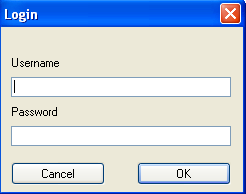
\includegraphics[scale=0.5]{frmLoginForm_scrot}
	\makeatletter
\def\PY@reset{\let\PY@it=\relax \let\PY@bf=\relax%
    \let\PY@ul=\relax \let\PY@tc=\relax%
    \let\PY@bc=\relax \let\PY@ff=\relax}
\def\PY@tok#1{\csname PY@tok@#1\endcsname}
\def\PY@toks#1+{\ifx\relax#1\empty\else%
    \PY@tok{#1}\expandafter\PY@toks\fi}
\def\PY@do#1{\PY@bc{\PY@tc{\PY@ul{%
    \PY@it{\PY@bf{\PY@ff{#1}}}}}}}
\def\PY#1#2{\PY@reset\PY@toks#1+\relax+\PY@do{#2}}

\expandafter\def\csname PY@tok@gd\endcsname{\def\PY@tc##1{\textcolor[rgb]{0.63,0.00,0.00}{##1}}}
\expandafter\def\csname PY@tok@gu\endcsname{\let\PY@bf=\textbf\def\PY@tc##1{\textcolor[rgb]{0.50,0.00,0.50}{##1}}}
\expandafter\def\csname PY@tok@gt\endcsname{\def\PY@tc##1{\textcolor[rgb]{0.00,0.25,0.82}{##1}}}
\expandafter\def\csname PY@tok@gs\endcsname{\let\PY@bf=\textbf}
\expandafter\def\csname PY@tok@gr\endcsname{\def\PY@tc##1{\textcolor[rgb]{1.00,0.00,0.00}{##1}}}
\expandafter\def\csname PY@tok@cm\endcsname{\let\PY@it=\textit\def\PY@tc##1{\textcolor[rgb]{0.25,0.50,0.50}{##1}}}
\expandafter\def\csname PY@tok@vg\endcsname{\def\PY@tc##1{\textcolor[rgb]{0.10,0.09,0.49}{##1}}}
\expandafter\def\csname PY@tok@m\endcsname{\def\PY@tc##1{\textcolor[rgb]{0.40,0.40,0.40}{##1}}}
\expandafter\def\csname PY@tok@mh\endcsname{\def\PY@tc##1{\textcolor[rgb]{0.40,0.40,0.40}{##1}}}
\expandafter\def\csname PY@tok@go\endcsname{\def\PY@tc##1{\textcolor[rgb]{0.50,0.50,0.50}{##1}}}
\expandafter\def\csname PY@tok@ge\endcsname{\let\PY@it=\textit}
\expandafter\def\csname PY@tok@vc\endcsname{\def\PY@tc##1{\textcolor[rgb]{0.10,0.09,0.49}{##1}}}
\expandafter\def\csname PY@tok@il\endcsname{\def\PY@tc##1{\textcolor[rgb]{0.40,0.40,0.40}{##1}}}
\expandafter\def\csname PY@tok@cs\endcsname{\let\PY@it=\textit\def\PY@tc##1{\textcolor[rgb]{0.25,0.50,0.50}{##1}}}
\expandafter\def\csname PY@tok@cp\endcsname{\def\PY@tc##1{\textcolor[rgb]{0.74,0.48,0.00}{##1}}}
\expandafter\def\csname PY@tok@gi\endcsname{\def\PY@tc##1{\textcolor[rgb]{0.00,0.63,0.00}{##1}}}
\expandafter\def\csname PY@tok@gh\endcsname{\let\PY@bf=\textbf\def\PY@tc##1{\textcolor[rgb]{0.00,0.00,0.50}{##1}}}
\expandafter\def\csname PY@tok@ni\endcsname{\let\PY@bf=\textbf\def\PY@tc##1{\textcolor[rgb]{0.60,0.60,0.60}{##1}}}
\expandafter\def\csname PY@tok@nl\endcsname{\def\PY@tc##1{\textcolor[rgb]{0.63,0.63,0.00}{##1}}}
\expandafter\def\csname PY@tok@nn\endcsname{\let\PY@bf=\textbf\def\PY@tc##1{\textcolor[rgb]{0.00,0.00,1.00}{##1}}}
\expandafter\def\csname PY@tok@no\endcsname{\def\PY@tc##1{\textcolor[rgb]{0.53,0.00,0.00}{##1}}}
\expandafter\def\csname PY@tok@na\endcsname{\def\PY@tc##1{\textcolor[rgb]{0.49,0.56,0.16}{##1}}}
\expandafter\def\csname PY@tok@nb\endcsname{\def\PY@tc##1{\textcolor[rgb]{0.00,0.50,0.00}{##1}}}
\expandafter\def\csname PY@tok@nc\endcsname{\let\PY@bf=\textbf\def\PY@tc##1{\textcolor[rgb]{0.00,0.00,1.00}{##1}}}
\expandafter\def\csname PY@tok@nd\endcsname{\def\PY@tc##1{\textcolor[rgb]{0.67,0.13,1.00}{##1}}}
\expandafter\def\csname PY@tok@ne\endcsname{\let\PY@bf=\textbf\def\PY@tc##1{\textcolor[rgb]{0.82,0.25,0.23}{##1}}}
\expandafter\def\csname PY@tok@nf\endcsname{\def\PY@tc##1{\textcolor[rgb]{0.00,0.00,1.00}{##1}}}
\expandafter\def\csname PY@tok@si\endcsname{\let\PY@bf=\textbf\def\PY@tc##1{\textcolor[rgb]{0.73,0.40,0.53}{##1}}}
\expandafter\def\csname PY@tok@s2\endcsname{\def\PY@tc##1{\textcolor[rgb]{0.73,0.13,0.13}{##1}}}
\expandafter\def\csname PY@tok@vi\endcsname{\def\PY@tc##1{\textcolor[rgb]{0.10,0.09,0.49}{##1}}}
\expandafter\def\csname PY@tok@nt\endcsname{\let\PY@bf=\textbf\def\PY@tc##1{\textcolor[rgb]{0.00,0.50,0.00}{##1}}}
\expandafter\def\csname PY@tok@nv\endcsname{\def\PY@tc##1{\textcolor[rgb]{0.10,0.09,0.49}{##1}}}
\expandafter\def\csname PY@tok@s1\endcsname{\def\PY@tc##1{\textcolor[rgb]{0.73,0.13,0.13}{##1}}}
\expandafter\def\csname PY@tok@sh\endcsname{\def\PY@tc##1{\textcolor[rgb]{0.73,0.13,0.13}{##1}}}
\expandafter\def\csname PY@tok@sc\endcsname{\def\PY@tc##1{\textcolor[rgb]{0.73,0.13,0.13}{##1}}}
\expandafter\def\csname PY@tok@sx\endcsname{\def\PY@tc##1{\textcolor[rgb]{0.00,0.50,0.00}{##1}}}
\expandafter\def\csname PY@tok@bp\endcsname{\def\PY@tc##1{\textcolor[rgb]{0.00,0.50,0.00}{##1}}}
\expandafter\def\csname PY@tok@c1\endcsname{\let\PY@it=\textit\def\PY@tc##1{\textcolor[rgb]{0.25,0.50,0.50}{##1}}}
\expandafter\def\csname PY@tok@kc\endcsname{\let\PY@bf=\textbf\def\PY@tc##1{\textcolor[rgb]{0.00,0.50,0.00}{##1}}}
\expandafter\def\csname PY@tok@c\endcsname{\let\PY@it=\textit\def\PY@tc##1{\textcolor[rgb]{0.25,0.50,0.50}{##1}}}
\expandafter\def\csname PY@tok@mf\endcsname{\def\PY@tc##1{\textcolor[rgb]{0.40,0.40,0.40}{##1}}}
\expandafter\def\csname PY@tok@err\endcsname{\def\PY@bc##1{\setlength{\fboxsep}{0pt}\fcolorbox[rgb]{1.00,0.00,0.00}{1,1,1}{\strut ##1}}}
\expandafter\def\csname PY@tok@kd\endcsname{\let\PY@bf=\textbf\def\PY@tc##1{\textcolor[rgb]{0.00,0.50,0.00}{##1}}}
\expandafter\def\csname PY@tok@ss\endcsname{\def\PY@tc##1{\textcolor[rgb]{0.10,0.09,0.49}{##1}}}
\expandafter\def\csname PY@tok@sr\endcsname{\def\PY@tc##1{\textcolor[rgb]{0.73,0.40,0.53}{##1}}}
\expandafter\def\csname PY@tok@mo\endcsname{\def\PY@tc##1{\textcolor[rgb]{0.40,0.40,0.40}{##1}}}
\expandafter\def\csname PY@tok@kn\endcsname{\let\PY@bf=\textbf\def\PY@tc##1{\textcolor[rgb]{0.00,0.50,0.00}{##1}}}
\expandafter\def\csname PY@tok@mi\endcsname{\def\PY@tc##1{\textcolor[rgb]{0.40,0.40,0.40}{##1}}}
\expandafter\def\csname PY@tok@gp\endcsname{\let\PY@bf=\textbf\def\PY@tc##1{\textcolor[rgb]{0.00,0.00,0.50}{##1}}}
\expandafter\def\csname PY@tok@o\endcsname{\def\PY@tc##1{\textcolor[rgb]{0.40,0.40,0.40}{##1}}}
\expandafter\def\csname PY@tok@kr\endcsname{\let\PY@bf=\textbf\def\PY@tc##1{\textcolor[rgb]{0.00,0.50,0.00}{##1}}}
\expandafter\def\csname PY@tok@s\endcsname{\def\PY@tc##1{\textcolor[rgb]{0.73,0.13,0.13}{##1}}}
\expandafter\def\csname PY@tok@kp\endcsname{\def\PY@tc##1{\textcolor[rgb]{0.00,0.50,0.00}{##1}}}
\expandafter\def\csname PY@tok@w\endcsname{\def\PY@tc##1{\textcolor[rgb]{0.73,0.73,0.73}{##1}}}
\expandafter\def\csname PY@tok@kt\endcsname{\def\PY@tc##1{\textcolor[rgb]{0.69,0.00,0.25}{##1}}}
\expandafter\def\csname PY@tok@ow\endcsname{\let\PY@bf=\textbf\def\PY@tc##1{\textcolor[rgb]{0.67,0.13,1.00}{##1}}}
\expandafter\def\csname PY@tok@sb\endcsname{\def\PY@tc##1{\textcolor[rgb]{0.73,0.13,0.13}{##1}}}
\expandafter\def\csname PY@tok@k\endcsname{\let\PY@bf=\textbf\def\PY@tc##1{\textcolor[rgb]{0.00,0.50,0.00}{##1}}}
\expandafter\def\csname PY@tok@se\endcsname{\let\PY@bf=\textbf\def\PY@tc##1{\textcolor[rgb]{0.73,0.40,0.13}{##1}}}
\expandafter\def\csname PY@tok@sd\endcsname{\let\PY@it=\textit\def\PY@tc##1{\textcolor[rgb]{0.73,0.13,0.13}{##1}}}

\def\PYZbs{\char`\\}
\def\PYZus{\char`\_}
\def\PYZob{\char`\{}
\def\PYZcb{\char`\}}
\def\PYZca{\char`\^}
\def\PYZam{\char`\&}
\def\PYZlt{\char`\<}
\def\PYZgt{\char`\>}
\def\PYZsh{\char`\#}
\def\PYZpc{\char`\%}
\def\PYZdl{\char`\$}
\def\PYZti{\char`\~}
% for compatibility with earlier versions
\def\PYZat{@}
\def\PYZlb{[}
\def\PYZrb{]}
\makeatother

\begin{Verbatim}[commandchars=\\\{\}]
\PY{err}{�}\PY{err}{�}\PY{err}{�}\PY{k}{Imports} \PY{n+nn}{System.Data}
\PY{k}{Imports} \PY{n+nn}{System.Data.OleDb}

\PY{k}{Public} \PY{k}{Class} \PY{n+nc}{frmLoginForm}
    \PY{k}{Public} \PY{n}{accConnection} \PY{o+ow}{As} \PY{k}{New} \PY{n}{OleDbConnection}
    \PY{c}{'Connect to the Microsoft Access database.}
    \PY{k}{Dim} \PY{n}{ConnectionString} \PY{o+ow}{As} \PY{k+kt}{String} \PY{o}{=} \PY{l+s}{"}\PY{l+s}{Provider=Microsoft.Jet.OLEDB.4.0;}\PY{l+s}{"} \PY{o}{\PYZam{}} \PY{n}{\PYZus{}}
            \PY{l+s}{"}\PY{l+s}{Data Source = E:\PYZbs{}SFS.mdb}\PY{l+s}{"}

    \PY{k}{Private} \PY{k}{Sub} \PY{n+nf}{frmLoginForm\PYZus{}Load}\PY{p}{(}\PY{k}{ByVal} \PY{n}{sender} \PY{o+ow}{As} \PY{n}{System}\PY{p}{.}\PY{n}{Object}\PY{p}{,} \PY{n}{\PYZus{}}
                                  \PY{k}{ByVal} \PY{n}{e} \PY{o+ow}{As} \PY{n}{System}\PY{p}{.}\PY{n}{EventArgs}\PY{p}{)} \PY{k}{Handles} \PY{k}{MyBase}\PY{p}{.}\PY{n}{Load}
        \PY{c}{'Connection variable.}
        \PY{n}{accConnection} \PY{o}{=} \PY{k}{New} \PY{n}{OleDbConnection}\PY{p}{(}\PY{n}{ConnectionString}\PY{p}{)}
    \PY{k}{End} \PY{k}{Sub}

    \PY{k}{Private} \PY{k}{Sub} \PY{n+nf}{OK\PYZus{}Click}\PY{p}{(}\PY{k}{ByVal} \PY{n}{sender} \PY{o+ow}{As} \PY{n}{System}\PY{p}{.}\PY{n}{Object}\PY{p}{,} \PY{n}{\PYZus{}}
                         \PY{k}{ByVal} \PY{n}{e} \PY{o+ow}{As} \PY{n}{System}\PY{p}{.}\PY{n}{EventArgs}\PY{p}{)} \PY{k}{Handles} \PY{n}{OK}\PY{p}{.}\PY{n}{Click}

        \PY{c}{'Get the login username and password from the database.}
        \PY{k}{Dim} \PY{n}{cmdString} \PY{o+ow}{As} \PY{k+kt}{String} \PY{o}{=} \PY{l+s}{"}\PY{l+s}{SELECT login\PYZus{}uname, login\PYZus{}pword FROM Login}\PY{l+s}{"}
        \PY{k}{Dim} \PY{n}{da} \PY{o+ow}{As} \PY{k}{New} \PY{n}{OleDbDataAdapter}\PY{p}{(}\PY{n}{cmdString}\PY{p}{,} \PY{n}{accConnection}\PY{p}{)}
        \PY{k}{Dim} \PY{n}{ds} \PY{o+ow}{As} \PY{k}{New} \PY{n}{DataSet}
        \PY{k}{Dim} \PY{n}{u} \PY{o+ow}{As} \PY{k+kt}{String} \PY{o}{=} \PY{n}{txtUsername}\PY{p}{.}\PY{n}{Text}
        \PY{k}{Dim} \PY{n}{p} \PY{o+ow}{As} \PY{k+kt}{String} \PY{o}{=} \PY{n}{txtPassword}\PY{p}{.}\PY{n}{Text}

        \PY{n}{da}\PY{p}{.}\PY{n}{Fill}\PY{p}{(}\PY{n}{ds}\PY{p}{,} \PY{l+s}{"}\PY{l+s}{Login}\PY{l+s}{"}\PY{p}{)}
        \PY{k}{Dim} \PY{n}{dt} \PY{o+ow}{As} \PY{n}{DataTable} \PY{o}{=} \PY{n}{ds}\PY{p}{.}\PY{n}{Tables}\PY{p}{(}\PY{l+m+mi}{0}\PY{p}{)}

        \PY{c}{'The usernames and passwords obtained from the database, to}
        \PY{c}{'compare with the ones the user entered.}
        \PY{k}{Dim} \PY{n}{loginuname} \PY{o+ow}{As} \PY{k+kt}{String} \PY{o}{=} \PY{l+s}{"}\PY{l+s}{"}
        \PY{k}{Dim} \PY{n}{loginpword} \PY{o+ow}{As} \PY{k+kt}{String} \PY{o}{=} \PY{l+s}{"}\PY{l+s}{"}

        \PY{k}{If} \PY{n}{ds}\PY{p}{.}\PY{n}{Tables}\PY{p}{(}\PY{l+m+mi}{0}\PY{p}{)}\PY{p}{.}\PY{n}{Rows}\PY{p}{.}\PY{n}{Count} \PY{o}{\PYZlt{}\PYZgt{}} \PY{l+m+mi}{0} \PY{k}{Then}
            \PY{n}{loginuname} \PY{o}{=} \PY{n}{ds}\PY{p}{.}\PY{n}{Tables}\PY{p}{(}\PY{l+m+mi}{0}\PY{p}{)}\PY{p}{.}\PY{n}{Rows}\PY{p}{(}\PY{l+m+mi}{0}\PY{p}{)}\PY{p}{.}\PY{n}{Item}\PY{p}{(}\PY{l+s}{"}\PY{l+s}{login\PYZus{}uname}\PY{l+s}{"}\PY{p}{)}
            \PY{n}{loginpword} \PY{o}{=} \PY{n}{ds}\PY{p}{.}\PY{n}{Tables}\PY{p}{(}\PY{l+m+mi}{0}\PY{p}{)}\PY{p}{.}\PY{n}{Rows}\PY{p}{(}\PY{l+m+mi}{0}\PY{p}{)}\PY{p}{.}\PY{n}{Item}\PY{p}{(}\PY{l+s}{"}\PY{l+s}{login\PYZus{}pword}\PY{l+s}{"}\PY{p}{)}
        \PY{k}{End} \PY{k}{If}

        \PY{k}{If} \PY{n}{u} \PY{o}{=} \PY{n}{loginuname} \PY{o+ow}{And} \PY{n}{p} \PY{o}{=} \PY{n}{loginpword} \PY{k}{Then}
            \PY{n}{frmMainMenu}\PY{p}{.}\PY{n}{Show}\PY{p}{(}\PY{p}{)}
        \PY{k}{Else}
            \PY{n}{MsgBox}\PY{p}{(}\PY{l+s}{"}\PY{l+s}{Incorrect username or password.  Try again.}\PY{l+s}{"}\PY{p}{)}
            \PY{c}{'Error, then blank the textboxes so that the user doesn't}
            \PY{c}{'have to.}
            \PY{n}{txtUsername}\PY{p}{.}\PY{n}{Text} \PY{o}{=} \PY{l+s}{"}\PY{l+s}{"}
            \PY{n}{txtPassword}\PY{p}{.}\PY{n}{Text} \PY{o}{=} \PY{l+s}{"}\PY{l+s}{"}
        \PY{k}{End} \PY{k}{If}

    \PY{k}{End} \PY{k}{Sub}

    \PY{k}{Private} \PY{k}{Sub} \PY{n+nf}{Cancel\PYZus{}Click}\PY{p}{(}\PY{k}{ByVal} \PY{n}{sender} \PY{o+ow}{As} \PY{n}{System}\PY{p}{.}\PY{n}{Object}\PY{p}{,} \PY{n}{\PYZus{}}
                             \PY{k}{ByVal} \PY{n}{e} \PY{o+ow}{As} \PY{n}{System}\PY{p}{.}\PY{n}{EventArgs}\PY{p}{)} \PY{k}{Handles} \PY{n}{Cancel}\PY{p}{.}\PY{n}{Click}
        \PY{k}{Me}\PY{p}{.}\PY{n}{Close}\PY{p}{(}\PY{p}{)}
    \PY{k}{End} \PY{k}{Sub}

\PY{k}{End} \PY{k}{Class}
\end{Verbatim}

\subsection{frmMainMenu}
	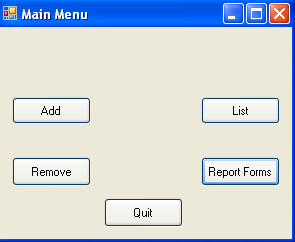
\includegraphics[scale=0.5]{frmMainMenu_scrot}
	\makeatletter
\def\PY@reset{\let\PY@it=\relax \let\PY@bf=\relax%
    \let\PY@ul=\relax \let\PY@tc=\relax%
    \let\PY@bc=\relax \let\PY@ff=\relax}
\def\PY@tok#1{\csname PY@tok@#1\endcsname}
\def\PY@toks#1+{\ifx\relax#1\empty\else%
    \PY@tok{#1}\expandafter\PY@toks\fi}
\def\PY@do#1{\PY@bc{\PY@tc{\PY@ul{%
    \PY@it{\PY@bf{\PY@ff{#1}}}}}}}
\def\PY#1#2{\PY@reset\PY@toks#1+\relax+\PY@do{#2}}

\expandafter\def\csname PY@tok@gd\endcsname{\def\PY@tc##1{\textcolor[rgb]{0.63,0.00,0.00}{##1}}}
\expandafter\def\csname PY@tok@gu\endcsname{\let\PY@bf=\textbf\def\PY@tc##1{\textcolor[rgb]{0.50,0.00,0.50}{##1}}}
\expandafter\def\csname PY@tok@gt\endcsname{\def\PY@tc##1{\textcolor[rgb]{0.00,0.25,0.82}{##1}}}
\expandafter\def\csname PY@tok@gs\endcsname{\let\PY@bf=\textbf}
\expandafter\def\csname PY@tok@gr\endcsname{\def\PY@tc##1{\textcolor[rgb]{1.00,0.00,0.00}{##1}}}
\expandafter\def\csname PY@tok@cm\endcsname{\let\PY@it=\textit\def\PY@tc##1{\textcolor[rgb]{0.25,0.50,0.50}{##1}}}
\expandafter\def\csname PY@tok@vg\endcsname{\def\PY@tc##1{\textcolor[rgb]{0.10,0.09,0.49}{##1}}}
\expandafter\def\csname PY@tok@m\endcsname{\def\PY@tc##1{\textcolor[rgb]{0.40,0.40,0.40}{##1}}}
\expandafter\def\csname PY@tok@mh\endcsname{\def\PY@tc##1{\textcolor[rgb]{0.40,0.40,0.40}{##1}}}
\expandafter\def\csname PY@tok@go\endcsname{\def\PY@tc##1{\textcolor[rgb]{0.50,0.50,0.50}{##1}}}
\expandafter\def\csname PY@tok@ge\endcsname{\let\PY@it=\textit}
\expandafter\def\csname PY@tok@vc\endcsname{\def\PY@tc##1{\textcolor[rgb]{0.10,0.09,0.49}{##1}}}
\expandafter\def\csname PY@tok@il\endcsname{\def\PY@tc##1{\textcolor[rgb]{0.40,0.40,0.40}{##1}}}
\expandafter\def\csname PY@tok@cs\endcsname{\let\PY@it=\textit\def\PY@tc##1{\textcolor[rgb]{0.25,0.50,0.50}{##1}}}
\expandafter\def\csname PY@tok@cp\endcsname{\def\PY@tc##1{\textcolor[rgb]{0.74,0.48,0.00}{##1}}}
\expandafter\def\csname PY@tok@gi\endcsname{\def\PY@tc##1{\textcolor[rgb]{0.00,0.63,0.00}{##1}}}
\expandafter\def\csname PY@tok@gh\endcsname{\let\PY@bf=\textbf\def\PY@tc##1{\textcolor[rgb]{0.00,0.00,0.50}{##1}}}
\expandafter\def\csname PY@tok@ni\endcsname{\let\PY@bf=\textbf\def\PY@tc##1{\textcolor[rgb]{0.60,0.60,0.60}{##1}}}
\expandafter\def\csname PY@tok@nl\endcsname{\def\PY@tc##1{\textcolor[rgb]{0.63,0.63,0.00}{##1}}}
\expandafter\def\csname PY@tok@nn\endcsname{\let\PY@bf=\textbf\def\PY@tc##1{\textcolor[rgb]{0.00,0.00,1.00}{##1}}}
\expandafter\def\csname PY@tok@no\endcsname{\def\PY@tc##1{\textcolor[rgb]{0.53,0.00,0.00}{##1}}}
\expandafter\def\csname PY@tok@na\endcsname{\def\PY@tc##1{\textcolor[rgb]{0.49,0.56,0.16}{##1}}}
\expandafter\def\csname PY@tok@nb\endcsname{\def\PY@tc##1{\textcolor[rgb]{0.00,0.50,0.00}{##1}}}
\expandafter\def\csname PY@tok@nc\endcsname{\let\PY@bf=\textbf\def\PY@tc##1{\textcolor[rgb]{0.00,0.00,1.00}{##1}}}
\expandafter\def\csname PY@tok@nd\endcsname{\def\PY@tc##1{\textcolor[rgb]{0.67,0.13,1.00}{##1}}}
\expandafter\def\csname PY@tok@ne\endcsname{\let\PY@bf=\textbf\def\PY@tc##1{\textcolor[rgb]{0.82,0.25,0.23}{##1}}}
\expandafter\def\csname PY@tok@nf\endcsname{\def\PY@tc##1{\textcolor[rgb]{0.00,0.00,1.00}{##1}}}
\expandafter\def\csname PY@tok@si\endcsname{\let\PY@bf=\textbf\def\PY@tc##1{\textcolor[rgb]{0.73,0.40,0.53}{##1}}}
\expandafter\def\csname PY@tok@s2\endcsname{\def\PY@tc##1{\textcolor[rgb]{0.73,0.13,0.13}{##1}}}
\expandafter\def\csname PY@tok@vi\endcsname{\def\PY@tc##1{\textcolor[rgb]{0.10,0.09,0.49}{##1}}}
\expandafter\def\csname PY@tok@nt\endcsname{\let\PY@bf=\textbf\def\PY@tc##1{\textcolor[rgb]{0.00,0.50,0.00}{##1}}}
\expandafter\def\csname PY@tok@nv\endcsname{\def\PY@tc##1{\textcolor[rgb]{0.10,0.09,0.49}{##1}}}
\expandafter\def\csname PY@tok@s1\endcsname{\def\PY@tc##1{\textcolor[rgb]{0.73,0.13,0.13}{##1}}}
\expandafter\def\csname PY@tok@sh\endcsname{\def\PY@tc##1{\textcolor[rgb]{0.73,0.13,0.13}{##1}}}
\expandafter\def\csname PY@tok@sc\endcsname{\def\PY@tc##1{\textcolor[rgb]{0.73,0.13,0.13}{##1}}}
\expandafter\def\csname PY@tok@sx\endcsname{\def\PY@tc##1{\textcolor[rgb]{0.00,0.50,0.00}{##1}}}
\expandafter\def\csname PY@tok@bp\endcsname{\def\PY@tc##1{\textcolor[rgb]{0.00,0.50,0.00}{##1}}}
\expandafter\def\csname PY@tok@c1\endcsname{\let\PY@it=\textit\def\PY@tc##1{\textcolor[rgb]{0.25,0.50,0.50}{##1}}}
\expandafter\def\csname PY@tok@kc\endcsname{\let\PY@bf=\textbf\def\PY@tc##1{\textcolor[rgb]{0.00,0.50,0.00}{##1}}}
\expandafter\def\csname PY@tok@c\endcsname{\let\PY@it=\textit\def\PY@tc##1{\textcolor[rgb]{0.25,0.50,0.50}{##1}}}
\expandafter\def\csname PY@tok@mf\endcsname{\def\PY@tc##1{\textcolor[rgb]{0.40,0.40,0.40}{##1}}}
\expandafter\def\csname PY@tok@err\endcsname{\def\PY@bc##1{\setlength{\fboxsep}{0pt}\fcolorbox[rgb]{1.00,0.00,0.00}{1,1,1}{\strut ##1}}}
\expandafter\def\csname PY@tok@kd\endcsname{\let\PY@bf=\textbf\def\PY@tc##1{\textcolor[rgb]{0.00,0.50,0.00}{##1}}}
\expandafter\def\csname PY@tok@ss\endcsname{\def\PY@tc##1{\textcolor[rgb]{0.10,0.09,0.49}{##1}}}
\expandafter\def\csname PY@tok@sr\endcsname{\def\PY@tc##1{\textcolor[rgb]{0.73,0.40,0.53}{##1}}}
\expandafter\def\csname PY@tok@mo\endcsname{\def\PY@tc##1{\textcolor[rgb]{0.40,0.40,0.40}{##1}}}
\expandafter\def\csname PY@tok@kn\endcsname{\let\PY@bf=\textbf\def\PY@tc##1{\textcolor[rgb]{0.00,0.50,0.00}{##1}}}
\expandafter\def\csname PY@tok@mi\endcsname{\def\PY@tc##1{\textcolor[rgb]{0.40,0.40,0.40}{##1}}}
\expandafter\def\csname PY@tok@gp\endcsname{\let\PY@bf=\textbf\def\PY@tc##1{\textcolor[rgb]{0.00,0.00,0.50}{##1}}}
\expandafter\def\csname PY@tok@o\endcsname{\def\PY@tc##1{\textcolor[rgb]{0.40,0.40,0.40}{##1}}}
\expandafter\def\csname PY@tok@kr\endcsname{\let\PY@bf=\textbf\def\PY@tc##1{\textcolor[rgb]{0.00,0.50,0.00}{##1}}}
\expandafter\def\csname PY@tok@s\endcsname{\def\PY@tc##1{\textcolor[rgb]{0.73,0.13,0.13}{##1}}}
\expandafter\def\csname PY@tok@kp\endcsname{\def\PY@tc##1{\textcolor[rgb]{0.00,0.50,0.00}{##1}}}
\expandafter\def\csname PY@tok@w\endcsname{\def\PY@tc##1{\textcolor[rgb]{0.73,0.73,0.73}{##1}}}
\expandafter\def\csname PY@tok@kt\endcsname{\def\PY@tc##1{\textcolor[rgb]{0.69,0.00,0.25}{##1}}}
\expandafter\def\csname PY@tok@ow\endcsname{\let\PY@bf=\textbf\def\PY@tc##1{\textcolor[rgb]{0.67,0.13,1.00}{##1}}}
\expandafter\def\csname PY@tok@sb\endcsname{\def\PY@tc##1{\textcolor[rgb]{0.73,0.13,0.13}{##1}}}
\expandafter\def\csname PY@tok@k\endcsname{\let\PY@bf=\textbf\def\PY@tc##1{\textcolor[rgb]{0.00,0.50,0.00}{##1}}}
\expandafter\def\csname PY@tok@se\endcsname{\let\PY@bf=\textbf\def\PY@tc##1{\textcolor[rgb]{0.73,0.40,0.13}{##1}}}
\expandafter\def\csname PY@tok@sd\endcsname{\let\PY@it=\textit\def\PY@tc##1{\textcolor[rgb]{0.73,0.13,0.13}{##1}}}

\def\PYZbs{\char`\\}
\def\PYZus{\char`\_}
\def\PYZob{\char`\{}
\def\PYZcb{\char`\}}
\def\PYZca{\char`\^}
\def\PYZam{\char`\&}
\def\PYZlt{\char`\<}
\def\PYZgt{\char`\>}
\def\PYZsh{\char`\#}
\def\PYZpc{\char`\%}
\def\PYZdl{\char`\$}
\def\PYZti{\char`\~}
% for compatibility with earlier versions
\def\PYZat{@}
\def\PYZlb{[}
\def\PYZrb{]}
\makeatother

\begin{Verbatim}[commandchars=\\\{\}]
\PY{err}{�}\PY{err}{�}\PY{err}{�}\PY{k}{Imports} \PY{n+nn}{System.Data}
\PY{k}{Imports} \PY{n+nn}{System.Data.OleDb}

\PY{k}{Public} \PY{k}{Class} \PY{n+nc}{frmMainMenu}

    \PY{c}{'THIS CODE SATISFIES SPECIFIC OBJECTIVE 1.}

    \PY{k}{Private} \PY{k}{Sub} \PY{n+nf}{frmMainMenu\PYZus{}Load}\PY{p}{(}\PY{k}{ByVal} \PY{n}{sender} \PY{o+ow}{As} \PY{n}{System}\PY{p}{.}\PY{n}{Object}\PY{p}{,} \PY{n}{\PYZus{}}
                                 \PY{k}{ByVal} \PY{n}{e} \PY{o+ow}{As} \PY{n}{System}\PY{p}{.}\PY{n}{EventArgs}\PY{p}{)} \PY{k}{Handles} \PY{k}{MyBase}\PY{p}{.}\PY{n}{Load}
        \PY{c}{'Hide the login form from the user when this form is loaded so}
        \PY{c}{'that he/she is not having to close a load of windows when he/she}
        \PY{c}{'quits the program.}
        \PY{n}{frmLoginForm}\PY{p}{.}\PY{n}{Hide}\PY{p}{(}\PY{p}{)}
    \PY{k}{End} \PY{k}{Sub}

    \PY{c}{'In each of these, according to the buttons clicked, show the correct}
    \PY{c}{'form and close this window.}
    \PY{k}{Private} \PY{k}{Sub} \PY{n+nf}{btnReport\PYZus{}Click}\PY{p}{(}\PY{k}{ByVal} \PY{n}{sender} \PY{o+ow}{As} \PY{n}{System}\PY{p}{.}\PY{n}{Object}\PY{p}{,} \PY{n}{\PYZus{}}
                                \PY{k}{ByVal} \PY{n}{e} \PY{o+ow}{As} \PY{n}{System}\PY{p}{.}\PY{n}{EventArgs}\PY{p}{)} \PY{k}{Handles} \PY{n}{btnReport}\PY{p}{.}\PY{n}{Click}
        \PY{k}{Me}\PY{p}{.}\PY{n}{Hide}\PY{p}{(}\PY{p}{)}
        \PY{n}{frmReportMenu}\PY{p}{.}\PY{n}{Show}\PY{p}{(}\PY{p}{)}
    \PY{k}{End} \PY{k}{Sub}

    \PY{k}{Private} \PY{k}{Sub} \PY{n+nf}{btnList\PYZus{}Click}\PY{p}{(}\PY{k}{ByVal} \PY{n}{sender} \PY{o+ow}{As} \PY{n}{System}\PY{p}{.}\PY{n}{Object}\PY{p}{,} \PY{n}{\PYZus{}}
                              \PY{k}{ByVal} \PY{n}{e} \PY{o+ow}{As} \PY{n}{System}\PY{p}{.}\PY{n}{EventArgs}\PY{p}{)} \PY{k}{Handles} \PY{n}{btnList}\PY{p}{.}\PY{n}{Click}
        \PY{k}{Me}\PY{p}{.}\PY{n}{Hide}\PY{p}{(}\PY{p}{)}
        \PY{n}{frmList}\PY{p}{.}\PY{n}{Show}\PY{p}{(}\PY{p}{)}
    \PY{k}{End} \PY{k}{Sub}

    \PY{k}{Private} \PY{k}{Sub} \PY{n+nf}{btnAdd\PYZus{}Click}\PY{p}{(}\PY{k}{ByVal} \PY{n}{sender} \PY{o+ow}{As} \PY{n}{System}\PY{p}{.}\PY{n}{Object}\PY{p}{,} \PY{n}{\PYZus{}}
                             \PY{k}{ByVal} \PY{n}{e} \PY{o+ow}{As} \PY{n}{System}\PY{p}{.}\PY{n}{EventArgs}\PY{p}{)} \PY{k}{Handles} \PY{n}{btnAdd}\PY{p}{.}\PY{n}{Click}
        \PY{k}{Me}\PY{p}{.}\PY{n}{Hide}\PY{p}{(}\PY{p}{)}
        \PY{n}{frmAdd}\PY{p}{.}\PY{n}{Show}\PY{p}{(}\PY{p}{)}
    \PY{k}{End} \PY{k}{Sub}

    \PY{k}{Private} \PY{k}{Sub} \PY{n+nf}{btnRemove\PYZus{}Click}\PY{p}{(}\PY{k}{ByVal} \PY{n}{sender} \PY{o+ow}{As} \PY{n}{System}\PY{p}{.}\PY{n}{Object}\PY{p}{,} \PY{n}{\PYZus{}}
                                \PY{k}{ByVal} \PY{n}{e} \PY{o+ow}{As} \PY{n}{System}\PY{p}{.}\PY{n}{EventArgs}\PY{p}{)} \PY{k}{Handles} \PY{n}{btnRemove}\PY{p}{.}\PY{n}{Click}
        \PY{k}{Me}\PY{p}{.}\PY{n}{Hide}\PY{p}{(}\PY{p}{)}
        \PY{n}{frmRemove}\PY{p}{.}\PY{n}{Show}\PY{p}{(}\PY{p}{)}
    \PY{k}{End} \PY{k}{Sub}

    \PY{k}{Private} \PY{k}{Sub} \PY{n+nf}{btnQuit\PYZus{}Click}\PY{p}{(}\PY{k}{ByVal} \PY{n}{sender} \PY{o+ow}{As} \PY{n}{System}\PY{p}{.}\PY{n}{Object}\PY{p}{,} \PY{n}{\PYZus{}}
                              \PY{k}{ByVal} \PY{n}{e} \PY{o+ow}{As} \PY{n}{System}\PY{p}{.}\PY{n}{EventArgs}\PY{p}{)} \PY{k}{Handles} \PY{n}{btnQuit}\PY{p}{.}\PY{n}{Click}
        \PY{k}{Me}\PY{p}{.}\PY{n}{Close}\PY{p}{(}\PY{p}{)}
        \PY{c}{'Now close the login form that is at present hidden so that the}
        \PY{c}{'program closes and doesn't stay running displaying nothing.  Also,}
        \PY{c}{'someone would have already logged in, so displaying the login}
        \PY{c}{'form again would intice people into logging in again, potentially}
        \PY{c}{'messing database stuff up like the closing of connections etc.}
        \PY{n}{frmLoginForm}\PY{p}{.}\PY{n}{Close}\PY{p}{(}\PY{p}{)}
    \PY{k}{End} \PY{k}{Sub}

\PY{k}{End} \PY{k}{Class}
\end{Verbatim}

\subsection{frmAdd}
	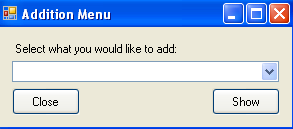
\includegraphics[scale=0.5]{frmAdd_scrot}
	\makeatletter
\def\PY@reset{\let\PY@it=\relax \let\PY@bf=\relax%
    \let\PY@ul=\relax \let\PY@tc=\relax%
    \let\PY@bc=\relax \let\PY@ff=\relax}
\def\PY@tok#1{\csname PY@tok@#1\endcsname}
\def\PY@toks#1+{\ifx\relax#1\empty\else%
    \PY@tok{#1}\expandafter\PY@toks\fi}
\def\PY@do#1{\PY@bc{\PY@tc{\PY@ul{%
    \PY@it{\PY@bf{\PY@ff{#1}}}}}}}
\def\PY#1#2{\PY@reset\PY@toks#1+\relax+\PY@do{#2}}

\expandafter\def\csname PY@tok@gd\endcsname{\def\PY@tc##1{\textcolor[rgb]{0.63,0.00,0.00}{##1}}}
\expandafter\def\csname PY@tok@gu\endcsname{\let\PY@bf=\textbf\def\PY@tc##1{\textcolor[rgb]{0.50,0.00,0.50}{##1}}}
\expandafter\def\csname PY@tok@gt\endcsname{\def\PY@tc##1{\textcolor[rgb]{0.00,0.25,0.82}{##1}}}
\expandafter\def\csname PY@tok@gs\endcsname{\let\PY@bf=\textbf}
\expandafter\def\csname PY@tok@gr\endcsname{\def\PY@tc##1{\textcolor[rgb]{1.00,0.00,0.00}{##1}}}
\expandafter\def\csname PY@tok@cm\endcsname{\let\PY@it=\textit\def\PY@tc##1{\textcolor[rgb]{0.25,0.50,0.50}{##1}}}
\expandafter\def\csname PY@tok@vg\endcsname{\def\PY@tc##1{\textcolor[rgb]{0.10,0.09,0.49}{##1}}}
\expandafter\def\csname PY@tok@m\endcsname{\def\PY@tc##1{\textcolor[rgb]{0.40,0.40,0.40}{##1}}}
\expandafter\def\csname PY@tok@mh\endcsname{\def\PY@tc##1{\textcolor[rgb]{0.40,0.40,0.40}{##1}}}
\expandafter\def\csname PY@tok@go\endcsname{\def\PY@tc##1{\textcolor[rgb]{0.50,0.50,0.50}{##1}}}
\expandafter\def\csname PY@tok@ge\endcsname{\let\PY@it=\textit}
\expandafter\def\csname PY@tok@vc\endcsname{\def\PY@tc##1{\textcolor[rgb]{0.10,0.09,0.49}{##1}}}
\expandafter\def\csname PY@tok@il\endcsname{\def\PY@tc##1{\textcolor[rgb]{0.40,0.40,0.40}{##1}}}
\expandafter\def\csname PY@tok@cs\endcsname{\let\PY@it=\textit\def\PY@tc##1{\textcolor[rgb]{0.25,0.50,0.50}{##1}}}
\expandafter\def\csname PY@tok@cp\endcsname{\def\PY@tc##1{\textcolor[rgb]{0.74,0.48,0.00}{##1}}}
\expandafter\def\csname PY@tok@gi\endcsname{\def\PY@tc##1{\textcolor[rgb]{0.00,0.63,0.00}{##1}}}
\expandafter\def\csname PY@tok@gh\endcsname{\let\PY@bf=\textbf\def\PY@tc##1{\textcolor[rgb]{0.00,0.00,0.50}{##1}}}
\expandafter\def\csname PY@tok@ni\endcsname{\let\PY@bf=\textbf\def\PY@tc##1{\textcolor[rgb]{0.60,0.60,0.60}{##1}}}
\expandafter\def\csname PY@tok@nl\endcsname{\def\PY@tc##1{\textcolor[rgb]{0.63,0.63,0.00}{##1}}}
\expandafter\def\csname PY@tok@nn\endcsname{\let\PY@bf=\textbf\def\PY@tc##1{\textcolor[rgb]{0.00,0.00,1.00}{##1}}}
\expandafter\def\csname PY@tok@no\endcsname{\def\PY@tc##1{\textcolor[rgb]{0.53,0.00,0.00}{##1}}}
\expandafter\def\csname PY@tok@na\endcsname{\def\PY@tc##1{\textcolor[rgb]{0.49,0.56,0.16}{##1}}}
\expandafter\def\csname PY@tok@nb\endcsname{\def\PY@tc##1{\textcolor[rgb]{0.00,0.50,0.00}{##1}}}
\expandafter\def\csname PY@tok@nc\endcsname{\let\PY@bf=\textbf\def\PY@tc##1{\textcolor[rgb]{0.00,0.00,1.00}{##1}}}
\expandafter\def\csname PY@tok@nd\endcsname{\def\PY@tc##1{\textcolor[rgb]{0.67,0.13,1.00}{##1}}}
\expandafter\def\csname PY@tok@ne\endcsname{\let\PY@bf=\textbf\def\PY@tc##1{\textcolor[rgb]{0.82,0.25,0.23}{##1}}}
\expandafter\def\csname PY@tok@nf\endcsname{\def\PY@tc##1{\textcolor[rgb]{0.00,0.00,1.00}{##1}}}
\expandafter\def\csname PY@tok@si\endcsname{\let\PY@bf=\textbf\def\PY@tc##1{\textcolor[rgb]{0.73,0.40,0.53}{##1}}}
\expandafter\def\csname PY@tok@s2\endcsname{\def\PY@tc##1{\textcolor[rgb]{0.73,0.13,0.13}{##1}}}
\expandafter\def\csname PY@tok@vi\endcsname{\def\PY@tc##1{\textcolor[rgb]{0.10,0.09,0.49}{##1}}}
\expandafter\def\csname PY@tok@nt\endcsname{\let\PY@bf=\textbf\def\PY@tc##1{\textcolor[rgb]{0.00,0.50,0.00}{##1}}}
\expandafter\def\csname PY@tok@nv\endcsname{\def\PY@tc##1{\textcolor[rgb]{0.10,0.09,0.49}{##1}}}
\expandafter\def\csname PY@tok@s1\endcsname{\def\PY@tc##1{\textcolor[rgb]{0.73,0.13,0.13}{##1}}}
\expandafter\def\csname PY@tok@sh\endcsname{\def\PY@tc##1{\textcolor[rgb]{0.73,0.13,0.13}{##1}}}
\expandafter\def\csname PY@tok@sc\endcsname{\def\PY@tc##1{\textcolor[rgb]{0.73,0.13,0.13}{##1}}}
\expandafter\def\csname PY@tok@sx\endcsname{\def\PY@tc##1{\textcolor[rgb]{0.00,0.50,0.00}{##1}}}
\expandafter\def\csname PY@tok@bp\endcsname{\def\PY@tc##1{\textcolor[rgb]{0.00,0.50,0.00}{##1}}}
\expandafter\def\csname PY@tok@c1\endcsname{\let\PY@it=\textit\def\PY@tc##1{\textcolor[rgb]{0.25,0.50,0.50}{##1}}}
\expandafter\def\csname PY@tok@kc\endcsname{\let\PY@bf=\textbf\def\PY@tc##1{\textcolor[rgb]{0.00,0.50,0.00}{##1}}}
\expandafter\def\csname PY@tok@c\endcsname{\let\PY@it=\textit\def\PY@tc##1{\textcolor[rgb]{0.25,0.50,0.50}{##1}}}
\expandafter\def\csname PY@tok@mf\endcsname{\def\PY@tc##1{\textcolor[rgb]{0.40,0.40,0.40}{##1}}}
\expandafter\def\csname PY@tok@err\endcsname{\def\PY@bc##1{\setlength{\fboxsep}{0pt}\fcolorbox[rgb]{1.00,0.00,0.00}{1,1,1}{\strut ##1}}}
\expandafter\def\csname PY@tok@kd\endcsname{\let\PY@bf=\textbf\def\PY@tc##1{\textcolor[rgb]{0.00,0.50,0.00}{##1}}}
\expandafter\def\csname PY@tok@ss\endcsname{\def\PY@tc##1{\textcolor[rgb]{0.10,0.09,0.49}{##1}}}
\expandafter\def\csname PY@tok@sr\endcsname{\def\PY@tc##1{\textcolor[rgb]{0.73,0.40,0.53}{##1}}}
\expandafter\def\csname PY@tok@mo\endcsname{\def\PY@tc##1{\textcolor[rgb]{0.40,0.40,0.40}{##1}}}
\expandafter\def\csname PY@tok@kn\endcsname{\let\PY@bf=\textbf\def\PY@tc##1{\textcolor[rgb]{0.00,0.50,0.00}{##1}}}
\expandafter\def\csname PY@tok@mi\endcsname{\def\PY@tc##1{\textcolor[rgb]{0.40,0.40,0.40}{##1}}}
\expandafter\def\csname PY@tok@gp\endcsname{\let\PY@bf=\textbf\def\PY@tc##1{\textcolor[rgb]{0.00,0.00,0.50}{##1}}}
\expandafter\def\csname PY@tok@o\endcsname{\def\PY@tc##1{\textcolor[rgb]{0.40,0.40,0.40}{##1}}}
\expandafter\def\csname PY@tok@kr\endcsname{\let\PY@bf=\textbf\def\PY@tc##1{\textcolor[rgb]{0.00,0.50,0.00}{##1}}}
\expandafter\def\csname PY@tok@s\endcsname{\def\PY@tc##1{\textcolor[rgb]{0.73,0.13,0.13}{##1}}}
\expandafter\def\csname PY@tok@kp\endcsname{\def\PY@tc##1{\textcolor[rgb]{0.00,0.50,0.00}{##1}}}
\expandafter\def\csname PY@tok@w\endcsname{\def\PY@tc##1{\textcolor[rgb]{0.73,0.73,0.73}{##1}}}
\expandafter\def\csname PY@tok@kt\endcsname{\def\PY@tc##1{\textcolor[rgb]{0.69,0.00,0.25}{##1}}}
\expandafter\def\csname PY@tok@ow\endcsname{\let\PY@bf=\textbf\def\PY@tc##1{\textcolor[rgb]{0.67,0.13,1.00}{##1}}}
\expandafter\def\csname PY@tok@sb\endcsname{\def\PY@tc##1{\textcolor[rgb]{0.73,0.13,0.13}{##1}}}
\expandafter\def\csname PY@tok@k\endcsname{\let\PY@bf=\textbf\def\PY@tc##1{\textcolor[rgb]{0.00,0.50,0.00}{##1}}}
\expandafter\def\csname PY@tok@se\endcsname{\let\PY@bf=\textbf\def\PY@tc##1{\textcolor[rgb]{0.73,0.40,0.13}{##1}}}
\expandafter\def\csname PY@tok@sd\endcsname{\let\PY@it=\textit\def\PY@tc##1{\textcolor[rgb]{0.73,0.13,0.13}{##1}}}

\def\PYZbs{\char`\\}
\def\PYZus{\char`\_}
\def\PYZob{\char`\{}
\def\PYZcb{\char`\}}
\def\PYZca{\char`\^}
\def\PYZam{\char`\&}
\def\PYZlt{\char`\<}
\def\PYZgt{\char`\>}
\def\PYZsh{\char`\#}
\def\PYZpc{\char`\%}
\def\PYZdl{\char`\$}
\def\PYZti{\char`\~}
% for compatibility with earlier versions
\def\PYZat{@}
\def\PYZlb{[}
\def\PYZrb{]}
\makeatother

\begin{Verbatim}[commandchars=\\\{\}]
\PY{err}{�}\PY{err}{�}\PY{err}{�}\PY{k}{Public} \PY{k}{Class} \PY{n+nc}{frmAdd}

    \PY{k}{Private} \PY{k}{Sub} \PY{n+nf}{frmAdd\PYZus{}Load}\PY{p}{(}\PY{k}{ByVal} \PY{n}{sender} \PY{o+ow}{As} \PY{n}{System}\PY{p}{.}\PY{n}{Object}\PY{p}{,} \PY{n}{\PYZus{}}
                            \PY{k}{ByVal} \PY{n}{e} \PY{o+ow}{As} \PY{n}{System}\PY{p}{.}\PY{n}{EventArgs}\PY{p}{)} \PY{k}{Handles} \PY{k}{MyBase}\PY{p}{.}\PY{n}{Load}
        \PY{c}{'Check if the database connection is breathing.}
        \PY{c}{'If it isn't, resuscitate it.  :)}
        \PY{k}{If} \PY{n}{frmLoginForm}\PY{p}{.}\PY{n}{accConnection}\PY{p}{.}\PY{n}{State} \PY{o}{\PYZlt{}\PYZgt{}} \PY{n}{ConnectionState}\PY{p}{.}\PY{n}{Open} \PY{k}{Then}
            \PY{n}{frmLoginForm}\PY{p}{.}\PY{n}{accConnection}\PY{p}{.}\PY{n}{Open}\PY{p}{(}\PY{p}{)}
        \PY{k}{End} \PY{k}{If}

        \PY{c}{'Populate drop down box.}
        \PY{n}{cbtxtAddOptions}\PY{p}{.}\PY{n}{Items}\PY{p}{.}\PY{n}{Add}\PY{p}{(}\PY{l+s}{"}\PY{l+s}{Customer}\PY{l+s}{"}\PY{p}{)}
        \PY{n}{cbtxtAddOptions}\PY{p}{.}\PY{n}{Items}\PY{p}{.}\PY{n}{Add}\PY{p}{(}\PY{l+s}{"}\PY{l+s}{Supplier}\PY{l+s}{"}\PY{p}{)}
        \PY{n}{cbtxtAddOptions}\PY{p}{.}\PY{n}{Items}\PY{p}{.}\PY{n}{Add}\PY{p}{(}\PY{l+s}{"}\PY{l+s}{Component}\PY{l+s}{"}\PY{p}{)}
    \PY{k}{End} \PY{k}{Sub}

    \PY{k}{Private} \PY{k}{Sub} \PY{n+nf}{btnShow\PYZus{}Click}\PY{p}{(}\PY{k}{ByVal} \PY{n}{sender} \PY{o+ow}{As} \PY{n}{System}\PY{p}{.}\PY{n}{Object}\PY{p}{,} \PY{n}{\PYZus{}}
                              \PY{k}{ByVal} \PY{n}{e} \PY{o+ow}{As} \PY{n}{System}\PY{p}{.}\PY{n}{EventArgs}\PY{p}{)} \PY{k}{Handles} \PY{n}{btnShow}\PY{p}{.}\PY{n}{Click}

        \PY{c}{'According to the option selected, display the next form and hide}
        \PY{c}{'this one.}
        \PY{k}{If} \PY{n}{cbtxtAddOptions}\PY{p}{.}\PY{n}{Text} \PY{o}{=} \PY{l+s}{"}\PY{l+s}{Customer}\PY{l+s}{"} \PY{k}{Then}
            \PY{k}{Me}\PY{p}{.}\PY{n}{Hide}\PY{p}{(}\PY{p}{)}
            \PY{n}{frmAddCustomer}\PY{p}{.}\PY{n}{Show}\PY{p}{(}\PY{p}{)}
        \PY{k}{ElseIf} \PY{n}{cbtxtAddOptions}\PY{p}{.}\PY{n}{Text} \PY{o}{=} \PY{l+s}{"}\PY{l+s}{Supplier}\PY{l+s}{"} \PY{k}{Then}
            \PY{k}{Me}\PY{p}{.}\PY{n}{Hide}\PY{p}{(}\PY{p}{)}
            \PY{n}{frmAddSupplier}\PY{p}{.}\PY{n}{Show}\PY{p}{(}\PY{p}{)}
        \PY{k}{ElseIf} \PY{n}{cbtxtAddOptions}\PY{p}{.}\PY{n}{Text} \PY{o}{=} \PY{l+s}{"}\PY{l+s}{Component}\PY{l+s}{"} \PY{k}{Then}
            \PY{k}{Me}\PY{p}{.}\PY{n}{Hide}\PY{p}{(}\PY{p}{)}
            \PY{n}{frmAddComponent}\PY{p}{.}\PY{n}{Show}\PY{p}{(}\PY{p}{)}
        \PY{k}{End} \PY{k}{If}
    \PY{k}{End} \PY{k}{Sub}

    \PY{k}{Private} \PY{k}{Sub} \PY{n+nf}{btnClose\PYZus{}Click}\PY{p}{(}\PY{k}{ByVal} \PY{n}{sender} \PY{o+ow}{As} \PY{n}{System}\PY{p}{.}\PY{n}{Object}\PY{p}{,} \PY{n}{\PYZus{}}
                               \PY{k}{ByVal} \PY{n}{e} \PY{o+ow}{As} \PY{n}{System}\PY{p}{.}\PY{n}{EventArgs}\PY{p}{)} \PY{k}{Handles} \PY{n}{btnClose}\PY{p}{.}\PY{n}{Click}
        \PY{c}{'Close this window and show the main menu.}
        \PY{k}{Me}\PY{p}{.}\PY{n}{Close}\PY{p}{(}\PY{p}{)}
        \PY{n}{frmMainMenu}\PY{p}{.}\PY{n}{Show}\PY{p}{(}\PY{p}{)}
    \PY{k}{End} \PY{k}{Sub}

\PY{k}{End} \PY{k}{Class}
\end{Verbatim}

\subsection{frmAddCustomer}
	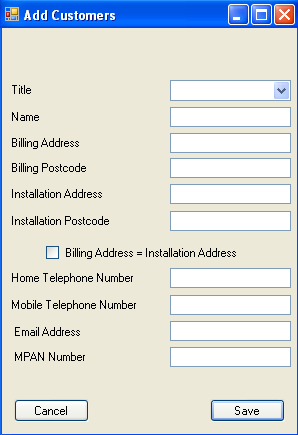
\includegraphics[scale=0.5]{frmAddCustomer_scrot}
	\makeatletter
\def\PY@reset{\let\PY@it=\relax \let\PY@bf=\relax%
    \let\PY@ul=\relax \let\PY@tc=\relax%
    \let\PY@bc=\relax \let\PY@ff=\relax}
\def\PY@tok#1{\csname PY@tok@#1\endcsname}
\def\PY@toks#1+{\ifx\relax#1\empty\else%
    \PY@tok{#1}\expandafter\PY@toks\fi}
\def\PY@do#1{\PY@bc{\PY@tc{\PY@ul{%
    \PY@it{\PY@bf{\PY@ff{#1}}}}}}}
\def\PY#1#2{\PY@reset\PY@toks#1+\relax+\PY@do{#2}}

\expandafter\def\csname PY@tok@gd\endcsname{\def\PY@tc##1{\textcolor[rgb]{0.63,0.00,0.00}{##1}}}
\expandafter\def\csname PY@tok@gu\endcsname{\let\PY@bf=\textbf\def\PY@tc##1{\textcolor[rgb]{0.50,0.00,0.50}{##1}}}
\expandafter\def\csname PY@tok@gt\endcsname{\def\PY@tc##1{\textcolor[rgb]{0.00,0.25,0.82}{##1}}}
\expandafter\def\csname PY@tok@gs\endcsname{\let\PY@bf=\textbf}
\expandafter\def\csname PY@tok@gr\endcsname{\def\PY@tc##1{\textcolor[rgb]{1.00,0.00,0.00}{##1}}}
\expandafter\def\csname PY@tok@cm\endcsname{\let\PY@it=\textit\def\PY@tc##1{\textcolor[rgb]{0.25,0.50,0.50}{##1}}}
\expandafter\def\csname PY@tok@vg\endcsname{\def\PY@tc##1{\textcolor[rgb]{0.10,0.09,0.49}{##1}}}
\expandafter\def\csname PY@tok@m\endcsname{\def\PY@tc##1{\textcolor[rgb]{0.40,0.40,0.40}{##1}}}
\expandafter\def\csname PY@tok@mh\endcsname{\def\PY@tc##1{\textcolor[rgb]{0.40,0.40,0.40}{##1}}}
\expandafter\def\csname PY@tok@go\endcsname{\def\PY@tc##1{\textcolor[rgb]{0.50,0.50,0.50}{##1}}}
\expandafter\def\csname PY@tok@ge\endcsname{\let\PY@it=\textit}
\expandafter\def\csname PY@tok@vc\endcsname{\def\PY@tc##1{\textcolor[rgb]{0.10,0.09,0.49}{##1}}}
\expandafter\def\csname PY@tok@il\endcsname{\def\PY@tc##1{\textcolor[rgb]{0.40,0.40,0.40}{##1}}}
\expandafter\def\csname PY@tok@cs\endcsname{\let\PY@it=\textit\def\PY@tc##1{\textcolor[rgb]{0.25,0.50,0.50}{##1}}}
\expandafter\def\csname PY@tok@cp\endcsname{\def\PY@tc##1{\textcolor[rgb]{0.74,0.48,0.00}{##1}}}
\expandafter\def\csname PY@tok@gi\endcsname{\def\PY@tc##1{\textcolor[rgb]{0.00,0.63,0.00}{##1}}}
\expandafter\def\csname PY@tok@gh\endcsname{\let\PY@bf=\textbf\def\PY@tc##1{\textcolor[rgb]{0.00,0.00,0.50}{##1}}}
\expandafter\def\csname PY@tok@ni\endcsname{\let\PY@bf=\textbf\def\PY@tc##1{\textcolor[rgb]{0.60,0.60,0.60}{##1}}}
\expandafter\def\csname PY@tok@nl\endcsname{\def\PY@tc##1{\textcolor[rgb]{0.63,0.63,0.00}{##1}}}
\expandafter\def\csname PY@tok@nn\endcsname{\let\PY@bf=\textbf\def\PY@tc##1{\textcolor[rgb]{0.00,0.00,1.00}{##1}}}
\expandafter\def\csname PY@tok@no\endcsname{\def\PY@tc##1{\textcolor[rgb]{0.53,0.00,0.00}{##1}}}
\expandafter\def\csname PY@tok@na\endcsname{\def\PY@tc##1{\textcolor[rgb]{0.49,0.56,0.16}{##1}}}
\expandafter\def\csname PY@tok@nb\endcsname{\def\PY@tc##1{\textcolor[rgb]{0.00,0.50,0.00}{##1}}}
\expandafter\def\csname PY@tok@nc\endcsname{\let\PY@bf=\textbf\def\PY@tc##1{\textcolor[rgb]{0.00,0.00,1.00}{##1}}}
\expandafter\def\csname PY@tok@nd\endcsname{\def\PY@tc##1{\textcolor[rgb]{0.67,0.13,1.00}{##1}}}
\expandafter\def\csname PY@tok@ne\endcsname{\let\PY@bf=\textbf\def\PY@tc##1{\textcolor[rgb]{0.82,0.25,0.23}{##1}}}
\expandafter\def\csname PY@tok@nf\endcsname{\def\PY@tc##1{\textcolor[rgb]{0.00,0.00,1.00}{##1}}}
\expandafter\def\csname PY@tok@si\endcsname{\let\PY@bf=\textbf\def\PY@tc##1{\textcolor[rgb]{0.73,0.40,0.53}{##1}}}
\expandafter\def\csname PY@tok@s2\endcsname{\def\PY@tc##1{\textcolor[rgb]{0.73,0.13,0.13}{##1}}}
\expandafter\def\csname PY@tok@vi\endcsname{\def\PY@tc##1{\textcolor[rgb]{0.10,0.09,0.49}{##1}}}
\expandafter\def\csname PY@tok@nt\endcsname{\let\PY@bf=\textbf\def\PY@tc##1{\textcolor[rgb]{0.00,0.50,0.00}{##1}}}
\expandafter\def\csname PY@tok@nv\endcsname{\def\PY@tc##1{\textcolor[rgb]{0.10,0.09,0.49}{##1}}}
\expandafter\def\csname PY@tok@s1\endcsname{\def\PY@tc##1{\textcolor[rgb]{0.73,0.13,0.13}{##1}}}
\expandafter\def\csname PY@tok@sh\endcsname{\def\PY@tc##1{\textcolor[rgb]{0.73,0.13,0.13}{##1}}}
\expandafter\def\csname PY@tok@sc\endcsname{\def\PY@tc##1{\textcolor[rgb]{0.73,0.13,0.13}{##1}}}
\expandafter\def\csname PY@tok@sx\endcsname{\def\PY@tc##1{\textcolor[rgb]{0.00,0.50,0.00}{##1}}}
\expandafter\def\csname PY@tok@bp\endcsname{\def\PY@tc##1{\textcolor[rgb]{0.00,0.50,0.00}{##1}}}
\expandafter\def\csname PY@tok@c1\endcsname{\let\PY@it=\textit\def\PY@tc##1{\textcolor[rgb]{0.25,0.50,0.50}{##1}}}
\expandafter\def\csname PY@tok@kc\endcsname{\let\PY@bf=\textbf\def\PY@tc##1{\textcolor[rgb]{0.00,0.50,0.00}{##1}}}
\expandafter\def\csname PY@tok@c\endcsname{\let\PY@it=\textit\def\PY@tc##1{\textcolor[rgb]{0.25,0.50,0.50}{##1}}}
\expandafter\def\csname PY@tok@mf\endcsname{\def\PY@tc##1{\textcolor[rgb]{0.40,0.40,0.40}{##1}}}
\expandafter\def\csname PY@tok@err\endcsname{\def\PY@bc##1{\setlength{\fboxsep}{0pt}\fcolorbox[rgb]{1.00,0.00,0.00}{1,1,1}{\strut ##1}}}
\expandafter\def\csname PY@tok@kd\endcsname{\let\PY@bf=\textbf\def\PY@tc##1{\textcolor[rgb]{0.00,0.50,0.00}{##1}}}
\expandafter\def\csname PY@tok@ss\endcsname{\def\PY@tc##1{\textcolor[rgb]{0.10,0.09,0.49}{##1}}}
\expandafter\def\csname PY@tok@sr\endcsname{\def\PY@tc##1{\textcolor[rgb]{0.73,0.40,0.53}{##1}}}
\expandafter\def\csname PY@tok@mo\endcsname{\def\PY@tc##1{\textcolor[rgb]{0.40,0.40,0.40}{##1}}}
\expandafter\def\csname PY@tok@kn\endcsname{\let\PY@bf=\textbf\def\PY@tc##1{\textcolor[rgb]{0.00,0.50,0.00}{##1}}}
\expandafter\def\csname PY@tok@mi\endcsname{\def\PY@tc##1{\textcolor[rgb]{0.40,0.40,0.40}{##1}}}
\expandafter\def\csname PY@tok@gp\endcsname{\let\PY@bf=\textbf\def\PY@tc##1{\textcolor[rgb]{0.00,0.00,0.50}{##1}}}
\expandafter\def\csname PY@tok@o\endcsname{\def\PY@tc##1{\textcolor[rgb]{0.40,0.40,0.40}{##1}}}
\expandafter\def\csname PY@tok@kr\endcsname{\let\PY@bf=\textbf\def\PY@tc##1{\textcolor[rgb]{0.00,0.50,0.00}{##1}}}
\expandafter\def\csname PY@tok@s\endcsname{\def\PY@tc##1{\textcolor[rgb]{0.73,0.13,0.13}{##1}}}
\expandafter\def\csname PY@tok@kp\endcsname{\def\PY@tc##1{\textcolor[rgb]{0.00,0.50,0.00}{##1}}}
\expandafter\def\csname PY@tok@w\endcsname{\def\PY@tc##1{\textcolor[rgb]{0.73,0.73,0.73}{##1}}}
\expandafter\def\csname PY@tok@kt\endcsname{\def\PY@tc##1{\textcolor[rgb]{0.69,0.00,0.25}{##1}}}
\expandafter\def\csname PY@tok@ow\endcsname{\let\PY@bf=\textbf\def\PY@tc##1{\textcolor[rgb]{0.67,0.13,1.00}{##1}}}
\expandafter\def\csname PY@tok@sb\endcsname{\def\PY@tc##1{\textcolor[rgb]{0.73,0.13,0.13}{##1}}}
\expandafter\def\csname PY@tok@k\endcsname{\let\PY@bf=\textbf\def\PY@tc##1{\textcolor[rgb]{0.00,0.50,0.00}{##1}}}
\expandafter\def\csname PY@tok@se\endcsname{\let\PY@bf=\textbf\def\PY@tc##1{\textcolor[rgb]{0.73,0.40,0.13}{##1}}}
\expandafter\def\csname PY@tok@sd\endcsname{\let\PY@it=\textit\def\PY@tc##1{\textcolor[rgb]{0.73,0.13,0.13}{##1}}}

\def\PYZbs{\char`\\}
\def\PYZus{\char`\_}
\def\PYZob{\char`\{}
\def\PYZcb{\char`\}}
\def\PYZca{\char`\^}
\def\PYZam{\char`\&}
\def\PYZlt{\char`\<}
\def\PYZgt{\char`\>}
\def\PYZsh{\char`\#}
\def\PYZpc{\char`\%}
\def\PYZdl{\char`\$}
\def\PYZti{\char`\~}
% for compatibility with earlier versions
\def\PYZat{@}
\def\PYZlb{[}
\def\PYZrb{]}
\makeatother

\begin{Verbatim}[commandchars=\\\{\}]
\PY{err}{�}\PY{err}{�}\PY{err}{�}\PY{k}{Imports} \PY{n+nn}{System.Data}
\PY{k}{Imports} \PY{n+nn}{System.Data.OleDb}

\PY{k}{Public} \PY{k}{Class} \PY{n+nc}{frmAddCustomer}
    \PY{c}{'THIS CODE SATISFIES SPECIFIC OBJECTIVE 3.}
    \PY{k}{Public} \PY{n}{accConnection} \PY{o+ow}{As} \PY{k}{New} \PY{n}{OleDbConnection}

    \PY{k}{Private} \PY{k}{Sub} \PY{n+nf}{frmAddCustomers\PYZus{}Load}\PY{p}{(}\PY{k}{ByVal} \PY{n}{sender} \PY{o+ow}{As} \PY{n}{System}\PY{p}{.}\PY{n}{Object}\PY{p}{,} \PY{n}{\PYZus{}}
                                     \PY{k}{ByVal} \PY{n}{e} \PY{o+ow}{As} \PY{n}{System}\PY{p}{.}\PY{n}{EventArgs}\PY{p}{)} \PY{k}{Handles} \PY{k}{MyBase}\PY{p}{.}\PY{n}{Load}
        \PY{c}{'Check if the database connection from the login form is still}
        \PY{c}{'alive - if it isn't, resuscitate (reopen) it.}
        \PY{k}{If} \PY{n}{frmLoginForm}\PY{p}{.}\PY{n}{accConnection}\PY{p}{.}\PY{n}{State} \PY{o}{\PYZlt{}\PYZgt{}} \PY{n}{ConnectionState}\PY{p}{.}\PY{n}{Open} \PY{k}{Then}
            \PY{n}{frmLoginForm}\PY{p}{.}\PY{n}{accConnection}\PY{p}{.}\PY{n}{Open}\PY{p}{(}\PY{p}{)}
        \PY{k}{End} \PY{k}{If}

        \PY{c}{'Populate this list with selected titles.}
        \PY{k}{Me}\PY{p}{.}\PY{n}{cbCustomerTitle}\PY{p}{.}\PY{n}{Items}\PY{p}{.}\PY{n}{Add}\PY{p}{(}\PY{l+s}{"}\PY{l+s}{Mr}\PY{l+s}{"}\PY{p}{)}
        \PY{k}{Me}\PY{p}{.}\PY{n}{cbCustomerTitle}\PY{p}{.}\PY{n}{Items}\PY{p}{.}\PY{n}{Add}\PY{p}{(}\PY{l+s}{"}\PY{l+s}{Mrs}\PY{l+s}{"}\PY{p}{)}
        \PY{k}{Me}\PY{p}{.}\PY{n}{cbCustomerTitle}\PY{p}{.}\PY{n}{Items}\PY{p}{.}\PY{n}{Add}\PY{p}{(}\PY{l+s}{"}\PY{l+s}{Miss}\PY{l+s}{"}\PY{p}{)}
        \PY{k}{Me}\PY{p}{.}\PY{n}{cbCustomerTitle}\PY{p}{.}\PY{n}{Items}\PY{p}{.}\PY{n}{Add}\PY{p}{(}\PY{l+s}{"}\PY{l+s}{Dr}\PY{l+s}{"}\PY{p}{)}

        \PY{c}{'Add tooltip to lblCustomerName and txtCustomerName field }
        \PY{c}{'so that the user knows to add the name in a uniform way.}
        \PY{k}{Me}\PY{p}{.}\PY{n}{ttCustomerName}\PY{p}{.}\PY{n}{SetToolTip}\PY{p}{(}\PY{k}{Me}\PY{p}{.}\PY{n}{lblCustomerName}\PY{p}{,} \PY{n}{\PYZus{}}
                                     \PY{l+s}{"}\PY{l+s}{Name must be in the format 'Forename \PYZlt{}space\PYZgt{} Surname'.}\PY{l+s}{"}\PY{p}{)}
        \PY{k}{Me}\PY{p}{.}\PY{n}{ttCustomerName}\PY{p}{.}\PY{n}{SetToolTip}\PY{p}{(}\PY{k}{Me}\PY{p}{.}\PY{n}{txtCustomerName}\PY{p}{,} \PY{n}{\PYZus{}}
                                     \PY{l+s}{"}\PY{l+s}{Name must be in the format 'Forename \PYZlt{}space\PYZgt{} Surname'.}\PY{l+s}{"}\PY{p}{)}
    \PY{k}{End} \PY{k}{Sub}

    \PY{k}{Private} \PY{k}{Sub} \PY{n+nf}{btnSave\PYZus{}Click}\PY{p}{(}\PY{k}{ByVal} \PY{n}{sender} \PY{o+ow}{As} \PY{n}{System}\PY{p}{.}\PY{n}{Object}\PY{p}{,} \PY{n}{\PYZus{}}
                              \PY{k}{ByVal} \PY{n}{e} \PY{o+ow}{As} \PY{n}{System}\PY{p}{.}\PY{n}{EventArgs}\PY{p}{)} \PY{k}{Handles} \PY{n}{btnSave}\PY{p}{.}\PY{n}{Click}

        \PY{k}{Dim} \PY{n}{cmdString} \PY{o+ow}{As} \PY{k+kt}{String} \PY{o}{=} \PY{l+s}{"}\PY{l+s}{INSERT INTO Customer (cust\PYZus{}title, cust\PYZus{}name, }\PY{l+s}{"} \PY{n}{\PYZus{}}
                                  \PY{o}{\PYZam{}} \PY{l+s}{"}\PY{l+s}{cust\PYZus{}billaddress, cust\PYZus{}billpostcode, cust\PYZus{}instaddress, }\PY{l+s}{"} \PY{n}{\PYZus{}}
                                  \PY{o}{\PYZam{}} \PY{l+s}{"}\PY{l+s}{cust\PYZus{}instpostcode, cust\PYZus{}hometelno, cust\PYZus{}mobtelno, }\PY{l+s}{"} \PY{n}{\PYZus{}}
                                  \PY{o}{\PYZam{}} \PY{l+s}{"}\PY{l+s}{cust\PYZus{}email, cust\PYZus{}mpan) VALUES (@cust\PYZus{}title,@cust\PYZus{}name,}\PY{l+s}{"} \PY{n}{\PYZus{}}
                                  \PY{o}{\PYZam{}} \PY{l+s}{"}\PY{l+s}{@cust\PYZus{}billaddress,@cust\PYZus{}billpostcode,@cust\PYZus{}instaddress,}\PY{l+s}{"} \PY{n}{\PYZus{}}
                                  \PY{o}{\PYZam{}} \PY{l+s}{"}\PY{l+s}{@cust\PYZus{}instpostcode,@cust\PYZus{}hometelno,@cust\PYZus{}mobtelno,}\PY{l+s}{"} \PY{n}{\PYZus{}}
                                  \PY{o}{\PYZam{}} \PY{l+s}{"}\PY{l+s}{@cust\PYZus{}email,@cust\PYZus{}mpan)}\PY{l+s}{"}

        \PY{k}{Dim} \PY{n}{AddCustomerDataAdapter} \PY{o+ow}{As} \PY{k}{New} \PY{n}{OleDbDataAdapter}
        \PY{k}{Dim} \PY{n}{accCommand} \PY{o+ow}{As} \PY{k}{New} \PY{n}{OleDbCommand}
        \PY{k}{Dim} \PY{n}{intInsert} \PY{o+ow}{As} \PY{k+kt}{Integer}
        \PY{k}{Dim} \PY{n}{CustomerForename} \PY{o+ow}{As} \PY{k+kt}{String}

        \PY{n}{CustomerForename} \PY{o}{=} \PY{n}{txtCustomerName}\PY{p}{.}\PY{n}{Text}
        \PY{n}{accCommand}\PY{p}{.}\PY{n}{Connection} \PY{o}{=} \PY{n}{frmLoginForm}\PY{p}{.}\PY{n}{accConnection}
        \PY{n}{accCommand}\PY{p}{.}\PY{n}{CommandType} \PY{o}{=} \PY{n}{CommandType}\PY{p}{.}\PY{n}{Text}
        \PY{n}{accCommand}\PY{p}{.}\PY{n}{CommandText} \PY{o}{=} \PY{n}{cmdString}

        \PY{c}{'Make the customer bill address be the install address too if}
        \PY{c}{'the user ticks the box, and deactivate the installation address}
        \PY{c}{'textboxes.}
        \PY{k}{If} \PY{n}{cbCustomerBillInstallSameAddress}\PY{p}{.}\PY{n}{CheckState} \PY{o}{=} \PY{l+m+mi}{1} \PY{k}{Then}
            \PY{n}{txtCustomerInstAddress}\PY{p}{.}\PY{n}{Text} \PY{o}{=} \PY{n}{txtCustomerBillAddress}\PY{p}{.}\PY{n}{Text}
            \PY{n}{txtCustomerInstPostcode}\PY{p}{.}\PY{n}{Text} \PY{o}{=} \PY{n}{txtCustomerBillPostcode}\PY{p}{.}\PY{n}{Text}
            \PY{n}{txtCustomerInstAddress}\PY{p}{.}\PY{n}{Enabled} \PY{o}{=} \PY{k}{False}
            \PY{n}{txtCustomerInstPostcode}\PY{p}{.}\PY{n}{Enabled} \PY{o}{=} \PY{k}{False}
        \PY{k}{End} \PY{k}{If}

        \PY{c}{'Call the insertion checking and inserting procedure.}
        \PY{k}{Call} \PY{n}{InsertParameters}\PY{p}{(}\PY{n}{accCommand}\PY{p}{)}

        \PY{c}{'Variable to check for errors - True if one exists, False if not.}
        \PY{k}{Dim} \PY{n}{error\PYZus{}yes\PYZus{}no} \PY{o+ow}{As} \PY{k+kt}{Boolean}

        \PY{c}{'Check if the email textbox contains '@', therefore if it is a}
        \PY{c}{'valid email address.}
        \PY{k}{Dim} \PY{n}{pos} \PY{o+ow}{As} \PY{k+kt}{Integer}
        \PY{k}{Dim} \PY{n}{etb} \PY{o+ow}{As} \PY{k+kt}{String} \PY{o}{=} \PY{n}{txtCustomerEmail}\PY{p}{.}\PY{n}{Text} \PY{c}{'email textbox}
        \PY{k}{Dim} \PY{n}{atsymbol} \PY{o+ow}{As} \PY{k+kt}{String} \PY{o}{=} \PY{l+s}{"}\PY{l+s}{@}\PY{l+s}{"}
        \PY{n}{pos} \PY{o}{=} \PY{n}{InStr}\PY{p}{(}\PY{n}{etb}\PY{p}{,} \PY{n}{atsymbol}\PY{p}{)}
        \PY{k}{If} \PY{n}{pos} \PY{o}{=} \PY{l+m+mi}{0} \PY{k}{Then}
            \PY{n}{error\PYZus{}yes\PYZus{}no} \PY{o}{=} \PY{k}{True}
            \PY{n}{intInsert} \PY{o}{=} \PY{l+m+mi}{0}
            \PY{n}{MsgBox}\PY{p}{(}\PY{l+s}{"}\PY{l+s}{Input a valid email address!}\PY{l+s}{"}\PY{p}{)}
        \PY{k}{Else}
            \PY{n}{error\PYZus{}yes\PYZus{}no} \PY{o}{=} \PY{k}{False}
        \PY{k}{End} \PY{k}{If}

        \PY{c}{'Check if there are any errors.  If there aren't, send it through}
        \PY{c}{'to the database.  Check for blank textboxes.}
        \PY{k}{Try}
            \PY{k}{If} \PY{n}{error\PYZus{}yes\PYZus{}no} \PY{o}{=} \PY{k}{False} \PY{k}{Then}
                \PY{n}{intInsert} \PY{o}{=} \PY{n}{accCommand}\PY{p}{.}\PY{n}{ExecuteNonQuery}\PY{p}{(}\PY{p}{)}
                \PY{n}{btnSave}\PY{p}{.}\PY{n}{Enabled} \PY{o}{=} \PY{k}{False}
            \PY{k}{Else}
                \PY{n}{intInsert} \PY{o}{=} \PY{l+m+mi}{0}
                \PY{n}{MsgBox}\PY{p}{(}\PY{l+s}{"}\PY{l+s}{There has been an error.}\PY{l+s}{"}\PY{p}{)}
            \PY{k}{End} \PY{k}{If}
        \PY{k}{Catch} \PY{n}{ex} \PY{o+ow}{As} \PY{n}{Exception}
            \PY{n}{intInsert} \PY{o}{=} \PY{l+m+mi}{0}
            \PY{n}{MsgBox}\PY{p}{(}\PY{l+s}{"}\PY{l+s}{There has been an error.}\PY{l+s}{"}\PY{p}{)}
        \PY{k}{End} \PY{k}{Try}
    \PY{k}{End} \PY{k}{Sub}

    \PY{k}{Private} \PY{k}{Sub} \PY{n+nf}{InsertParameters}\PY{p}{(}\PY{k}{ByRef} \PY{n}{acccmd} \PY{o+ow}{As} \PY{n}{OleDbCommand}\PY{p}{)}
        \PY{c}{'Insert the data into the database.}

        \PY{n}{acccmd}\PY{p}{.}\PY{n}{Parameters}\PY{p}{.}\PY{n}{Add}\PY{p}{(}\PY{l+s}{"}\PY{l+s}{@cust\PYZus{}title}\PY{l+s}{"}\PY{p}{,} \PY{n}{OleDbType}\PY{p}{.}\PY{n}{Char}\PY{p}{)}\PY{p}{.}\PY{n}{Value} \PY{o}{=} \PY{n}{\PYZus{}}
                                \PY{n}{cbCustomerTitle}\PY{p}{.}\PY{n}{SelectedItem}
        \PY{n}{acccmd}\PY{p}{.}\PY{n}{Parameters}\PY{p}{.}\PY{n}{Add}\PY{p}{(}\PY{l+s}{"}\PY{l+s}{@cust\PYZus{}name}\PY{l+s}{"}\PY{p}{,} \PY{n}{OleDbType}\PY{p}{.}\PY{n}{Char}\PY{p}{)}\PY{p}{.}\PY{n}{Value} \PY{o}{=} \PY{n}{\PYZus{}}
                                \PY{n}{txtCustomerName}\PY{p}{.}\PY{n}{Text}
        \PY{n}{acccmd}\PY{p}{.}\PY{n}{Parameters}\PY{p}{.}\PY{n}{Add}\PY{p}{(}\PY{l+s}{"}\PY{l+s}{@cust\PYZus{}billaddress}\PY{l+s}{"}\PY{p}{,} \PY{n}{OleDbType}\PY{p}{.}\PY{n}{Char}\PY{p}{)}\PY{p}{.}\PY{n}{Value} \PY{o}{=} \PY{n}{\PYZus{}}
                                \PY{n}{txtCustomerBillAddress}\PY{p}{.}\PY{n}{Text}
        \PY{n}{acccmd}\PY{p}{.}\PY{n}{Parameters}\PY{p}{.}\PY{n}{Add}\PY{p}{(}\PY{l+s}{"}\PY{l+s}{@cust\PYZus{}billpostcode}\PY{l+s}{"}\PY{p}{,} \PY{n}{OleDbType}\PY{p}{.}\PY{n}{Char}\PY{p}{)}\PY{p}{.}\PY{n}{Value} \PY{o}{=} \PY{n}{\PYZus{}}
                                \PY{n}{txtCustomerBillPostcode}\PY{p}{.}\PY{n}{Text}
        \PY{n}{acccmd}\PY{p}{.}\PY{n}{Parameters}\PY{p}{.}\PY{n}{Add}\PY{p}{(}\PY{l+s}{"}\PY{l+s}{@cust\PYZus{}instaddress}\PY{l+s}{"}\PY{p}{,} \PY{n}{OleDbType}\PY{p}{.}\PY{n}{Char}\PY{p}{)}\PY{p}{.}\PY{n}{Value} \PY{o}{=} \PY{n}{\PYZus{}}
                                \PY{n}{txtCustomerInstAddress}\PY{p}{.}\PY{n}{Text}
        \PY{n}{acccmd}\PY{p}{.}\PY{n}{Parameters}\PY{p}{.}\PY{n}{Add}\PY{p}{(}\PY{l+s}{"}\PY{l+s}{@cust\PYZus{}instpostcode}\PY{l+s}{"}\PY{p}{,} \PY{n}{OleDbType}\PY{p}{.}\PY{n}{Char}\PY{p}{)}\PY{p}{.}\PY{n}{Value} \PY{o}{=} \PY{n}{\PYZus{}}
                                \PY{n}{txtCustomerInstPostcode}\PY{p}{.}\PY{n}{Text}
        \PY{n}{acccmd}\PY{p}{.}\PY{n}{Parameters}\PY{p}{.}\PY{n}{Add}\PY{p}{(}\PY{l+s}{"}\PY{l+s}{@cust\PYZus{}hometelno}\PY{l+s}{"}\PY{p}{,} \PY{n}{OleDbType}\PY{p}{.}\PY{n}{Char}\PY{p}{)}\PY{p}{.}\PY{n}{Value} \PY{o}{=} \PY{n}{\PYZus{}}
                                \PY{n}{txtCustomerHomeTelNo}\PY{p}{.}\PY{n}{Text}
        \PY{n}{acccmd}\PY{p}{.}\PY{n}{Parameters}\PY{p}{.}\PY{n}{Add}\PY{p}{(}\PY{l+s}{"}\PY{l+s}{@cust\PYZus{}mobtelno}\PY{l+s}{"}\PY{p}{,} \PY{n}{OleDbType}\PY{p}{.}\PY{n}{Char}\PY{p}{)}\PY{p}{.}\PY{n}{Value} \PY{o}{=} \PY{n}{\PYZus{}}
                                \PY{n}{mtxtCustomerMobTelNo}\PY{p}{.}\PY{n}{Text}
        \PY{n}{acccmd}\PY{p}{.}\PY{n}{Parameters}\PY{p}{.}\PY{n}{Add}\PY{p}{(}\PY{l+s}{"}\PY{l+s}{@cust\PYZus{}email}\PY{l+s}{"}\PY{p}{,} \PY{n}{OleDbType}\PY{p}{.}\PY{n}{Char}\PY{p}{)}\PY{p}{.}\PY{n}{Value} \PY{o}{=} \PY{n}{\PYZus{}}
                                \PY{n}{txtCustomerEmail}\PY{p}{.}\PY{n}{Text}
        \PY{n}{acccmd}\PY{p}{.}\PY{n}{Parameters}\PY{p}{.}\PY{n}{Add}\PY{p}{(}\PY{l+s}{"}\PY{l+s}{@cust\PYZus{}mpan}\PY{l+s}{"}\PY{p}{,} \PY{n}{OleDbType}\PY{p}{.}\PY{n}{Char}\PY{p}{)}\PY{p}{.}\PY{n}{Value} \PY{o}{=} \PY{n}{\PYZus{}}
                                \PY{n}{txtCustomerMpanNo}\PY{p}{.}\PY{n}{Text}
    \PY{k}{End} \PY{k}{Sub}

    \PY{k}{Private} \PY{k}{Sub} \PY{n+nf}{btnCancel\PYZus{}Click}\PY{p}{(}\PY{k}{ByVal} \PY{n}{sender} \PY{o+ow}{As} \PY{n}{System}\PY{p}{.}\PY{n}{Object}\PY{p}{,} \PY{n}{\PYZus{}}
                                \PY{k}{ByVal} \PY{n}{e} \PY{o+ow}{As} \PY{n}{System}\PY{p}{.}\PY{n}{EventArgs}\PY{p}{)} \PY{k}{Handles} \PY{n}{btnCancel}\PY{p}{.}\PY{n}{Click}

        \PY{k}{If} \PY{n}{btnSave}\PY{p}{.}\PY{n}{Enabled} \PY{o}{=} \PY{k}{False} \PY{k}{Then}
            \PY{c}{'It's all fine and has gone through OK, so don't display a}
            \PY{c}{'message because that would just be annoying, just close this}
            \PY{c}{'and display the previous form.}
            \PY{k}{Me}\PY{p}{.}\PY{n}{Close}\PY{p}{(}\PY{p}{)}
            \PY{n}{frmAdd}\PY{p}{.}\PY{n}{Show}\PY{p}{(}\PY{p}{)}
        \PY{k}{Else}
            \PY{c}{'If it hasn't gone through OK, or nothing has been added,}
            \PY{c}{'then let the user know this so as not to panic them;}
            \PY{c}{'if the user did not mean to click the button, he/she knows.}
            \PY{n}{MsgBox}\PY{p}{(}\PY{l+s}{"}\PY{l+s}{This window will close and these details will not be saved.}\PY{l+s}{"}\PY{p}{)}
            \PY{k}{Me}\PY{p}{.}\PY{n}{Close}\PY{p}{(}\PY{p}{)}
            \PY{n}{frmAdd}\PY{p}{.}\PY{n}{Show}\PY{p}{(}\PY{p}{)}
        \PY{k}{End} \PY{k}{If}

    \PY{k}{End} \PY{k}{Sub}
\PY{k}{End} \PY{k}{Class}
\end{Verbatim}
	
\subsection{frmAddSupplier}
	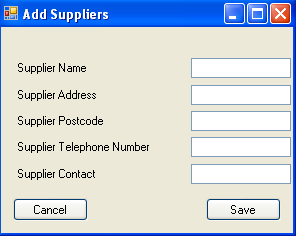
\includegraphics[scale=0.5]{frmAddSupplier_scrot}
	\makeatletter
\def\PY@reset{\let\PY@it=\relax \let\PY@bf=\relax%
    \let\PY@ul=\relax \let\PY@tc=\relax%
    \let\PY@bc=\relax \let\PY@ff=\relax}
\def\PY@tok#1{\csname PY@tok@#1\endcsname}
\def\PY@toks#1+{\ifx\relax#1\empty\else%
    \PY@tok{#1}\expandafter\PY@toks\fi}
\def\PY@do#1{\PY@bc{\PY@tc{\PY@ul{%
    \PY@it{\PY@bf{\PY@ff{#1}}}}}}}
\def\PY#1#2{\PY@reset\PY@toks#1+\relax+\PY@do{#2}}

\expandafter\def\csname PY@tok@gd\endcsname{\def\PY@tc##1{\textcolor[rgb]{0.63,0.00,0.00}{##1}}}
\expandafter\def\csname PY@tok@gu\endcsname{\let\PY@bf=\textbf\def\PY@tc##1{\textcolor[rgb]{0.50,0.00,0.50}{##1}}}
\expandafter\def\csname PY@tok@gt\endcsname{\def\PY@tc##1{\textcolor[rgb]{0.00,0.25,0.82}{##1}}}
\expandafter\def\csname PY@tok@gs\endcsname{\let\PY@bf=\textbf}
\expandafter\def\csname PY@tok@gr\endcsname{\def\PY@tc##1{\textcolor[rgb]{1.00,0.00,0.00}{##1}}}
\expandafter\def\csname PY@tok@cm\endcsname{\let\PY@it=\textit\def\PY@tc##1{\textcolor[rgb]{0.25,0.50,0.50}{##1}}}
\expandafter\def\csname PY@tok@vg\endcsname{\def\PY@tc##1{\textcolor[rgb]{0.10,0.09,0.49}{##1}}}
\expandafter\def\csname PY@tok@m\endcsname{\def\PY@tc##1{\textcolor[rgb]{0.40,0.40,0.40}{##1}}}
\expandafter\def\csname PY@tok@mh\endcsname{\def\PY@tc##1{\textcolor[rgb]{0.40,0.40,0.40}{##1}}}
\expandafter\def\csname PY@tok@go\endcsname{\def\PY@tc##1{\textcolor[rgb]{0.50,0.50,0.50}{##1}}}
\expandafter\def\csname PY@tok@ge\endcsname{\let\PY@it=\textit}
\expandafter\def\csname PY@tok@vc\endcsname{\def\PY@tc##1{\textcolor[rgb]{0.10,0.09,0.49}{##1}}}
\expandafter\def\csname PY@tok@il\endcsname{\def\PY@tc##1{\textcolor[rgb]{0.40,0.40,0.40}{##1}}}
\expandafter\def\csname PY@tok@cs\endcsname{\let\PY@it=\textit\def\PY@tc##1{\textcolor[rgb]{0.25,0.50,0.50}{##1}}}
\expandafter\def\csname PY@tok@cp\endcsname{\def\PY@tc##1{\textcolor[rgb]{0.74,0.48,0.00}{##1}}}
\expandafter\def\csname PY@tok@gi\endcsname{\def\PY@tc##1{\textcolor[rgb]{0.00,0.63,0.00}{##1}}}
\expandafter\def\csname PY@tok@gh\endcsname{\let\PY@bf=\textbf\def\PY@tc##1{\textcolor[rgb]{0.00,0.00,0.50}{##1}}}
\expandafter\def\csname PY@tok@ni\endcsname{\let\PY@bf=\textbf\def\PY@tc##1{\textcolor[rgb]{0.60,0.60,0.60}{##1}}}
\expandafter\def\csname PY@tok@nl\endcsname{\def\PY@tc##1{\textcolor[rgb]{0.63,0.63,0.00}{##1}}}
\expandafter\def\csname PY@tok@nn\endcsname{\let\PY@bf=\textbf\def\PY@tc##1{\textcolor[rgb]{0.00,0.00,1.00}{##1}}}
\expandafter\def\csname PY@tok@no\endcsname{\def\PY@tc##1{\textcolor[rgb]{0.53,0.00,0.00}{##1}}}
\expandafter\def\csname PY@tok@na\endcsname{\def\PY@tc##1{\textcolor[rgb]{0.49,0.56,0.16}{##1}}}
\expandafter\def\csname PY@tok@nb\endcsname{\def\PY@tc##1{\textcolor[rgb]{0.00,0.50,0.00}{##1}}}
\expandafter\def\csname PY@tok@nc\endcsname{\let\PY@bf=\textbf\def\PY@tc##1{\textcolor[rgb]{0.00,0.00,1.00}{##1}}}
\expandafter\def\csname PY@tok@nd\endcsname{\def\PY@tc##1{\textcolor[rgb]{0.67,0.13,1.00}{##1}}}
\expandafter\def\csname PY@tok@ne\endcsname{\let\PY@bf=\textbf\def\PY@tc##1{\textcolor[rgb]{0.82,0.25,0.23}{##1}}}
\expandafter\def\csname PY@tok@nf\endcsname{\def\PY@tc##1{\textcolor[rgb]{0.00,0.00,1.00}{##1}}}
\expandafter\def\csname PY@tok@si\endcsname{\let\PY@bf=\textbf\def\PY@tc##1{\textcolor[rgb]{0.73,0.40,0.53}{##1}}}
\expandafter\def\csname PY@tok@s2\endcsname{\def\PY@tc##1{\textcolor[rgb]{0.73,0.13,0.13}{##1}}}
\expandafter\def\csname PY@tok@vi\endcsname{\def\PY@tc##1{\textcolor[rgb]{0.10,0.09,0.49}{##1}}}
\expandafter\def\csname PY@tok@nt\endcsname{\let\PY@bf=\textbf\def\PY@tc##1{\textcolor[rgb]{0.00,0.50,0.00}{##1}}}
\expandafter\def\csname PY@tok@nv\endcsname{\def\PY@tc##1{\textcolor[rgb]{0.10,0.09,0.49}{##1}}}
\expandafter\def\csname PY@tok@s1\endcsname{\def\PY@tc##1{\textcolor[rgb]{0.73,0.13,0.13}{##1}}}
\expandafter\def\csname PY@tok@sh\endcsname{\def\PY@tc##1{\textcolor[rgb]{0.73,0.13,0.13}{##1}}}
\expandafter\def\csname PY@tok@sc\endcsname{\def\PY@tc##1{\textcolor[rgb]{0.73,0.13,0.13}{##1}}}
\expandafter\def\csname PY@tok@sx\endcsname{\def\PY@tc##1{\textcolor[rgb]{0.00,0.50,0.00}{##1}}}
\expandafter\def\csname PY@tok@bp\endcsname{\def\PY@tc##1{\textcolor[rgb]{0.00,0.50,0.00}{##1}}}
\expandafter\def\csname PY@tok@c1\endcsname{\let\PY@it=\textit\def\PY@tc##1{\textcolor[rgb]{0.25,0.50,0.50}{##1}}}
\expandafter\def\csname PY@tok@kc\endcsname{\let\PY@bf=\textbf\def\PY@tc##1{\textcolor[rgb]{0.00,0.50,0.00}{##1}}}
\expandafter\def\csname PY@tok@c\endcsname{\let\PY@it=\textit\def\PY@tc##1{\textcolor[rgb]{0.25,0.50,0.50}{##1}}}
\expandafter\def\csname PY@tok@mf\endcsname{\def\PY@tc##1{\textcolor[rgb]{0.40,0.40,0.40}{##1}}}
\expandafter\def\csname PY@tok@err\endcsname{\def\PY@bc##1{\setlength{\fboxsep}{0pt}\fcolorbox[rgb]{1.00,0.00,0.00}{1,1,1}{\strut ##1}}}
\expandafter\def\csname PY@tok@kd\endcsname{\let\PY@bf=\textbf\def\PY@tc##1{\textcolor[rgb]{0.00,0.50,0.00}{##1}}}
\expandafter\def\csname PY@tok@ss\endcsname{\def\PY@tc##1{\textcolor[rgb]{0.10,0.09,0.49}{##1}}}
\expandafter\def\csname PY@tok@sr\endcsname{\def\PY@tc##1{\textcolor[rgb]{0.73,0.40,0.53}{##1}}}
\expandafter\def\csname PY@tok@mo\endcsname{\def\PY@tc##1{\textcolor[rgb]{0.40,0.40,0.40}{##1}}}
\expandafter\def\csname PY@tok@kn\endcsname{\let\PY@bf=\textbf\def\PY@tc##1{\textcolor[rgb]{0.00,0.50,0.00}{##1}}}
\expandafter\def\csname PY@tok@mi\endcsname{\def\PY@tc##1{\textcolor[rgb]{0.40,0.40,0.40}{##1}}}
\expandafter\def\csname PY@tok@gp\endcsname{\let\PY@bf=\textbf\def\PY@tc##1{\textcolor[rgb]{0.00,0.00,0.50}{##1}}}
\expandafter\def\csname PY@tok@o\endcsname{\def\PY@tc##1{\textcolor[rgb]{0.40,0.40,0.40}{##1}}}
\expandafter\def\csname PY@tok@kr\endcsname{\let\PY@bf=\textbf\def\PY@tc##1{\textcolor[rgb]{0.00,0.50,0.00}{##1}}}
\expandafter\def\csname PY@tok@s\endcsname{\def\PY@tc##1{\textcolor[rgb]{0.73,0.13,0.13}{##1}}}
\expandafter\def\csname PY@tok@kp\endcsname{\def\PY@tc##1{\textcolor[rgb]{0.00,0.50,0.00}{##1}}}
\expandafter\def\csname PY@tok@w\endcsname{\def\PY@tc##1{\textcolor[rgb]{0.73,0.73,0.73}{##1}}}
\expandafter\def\csname PY@tok@kt\endcsname{\def\PY@tc##1{\textcolor[rgb]{0.69,0.00,0.25}{##1}}}
\expandafter\def\csname PY@tok@ow\endcsname{\let\PY@bf=\textbf\def\PY@tc##1{\textcolor[rgb]{0.67,0.13,1.00}{##1}}}
\expandafter\def\csname PY@tok@sb\endcsname{\def\PY@tc##1{\textcolor[rgb]{0.73,0.13,0.13}{##1}}}
\expandafter\def\csname PY@tok@k\endcsname{\let\PY@bf=\textbf\def\PY@tc##1{\textcolor[rgb]{0.00,0.50,0.00}{##1}}}
\expandafter\def\csname PY@tok@se\endcsname{\let\PY@bf=\textbf\def\PY@tc##1{\textcolor[rgb]{0.73,0.40,0.13}{##1}}}
\expandafter\def\csname PY@tok@sd\endcsname{\let\PY@it=\textit\def\PY@tc##1{\textcolor[rgb]{0.73,0.13,0.13}{##1}}}

\def\PYZbs{\char`\\}
\def\PYZus{\char`\_}
\def\PYZob{\char`\{}
\def\PYZcb{\char`\}}
\def\PYZca{\char`\^}
\def\PYZam{\char`\&}
\def\PYZlt{\char`\<}
\def\PYZgt{\char`\>}
\def\PYZsh{\char`\#}
\def\PYZpc{\char`\%}
\def\PYZdl{\char`\$}
\def\PYZti{\char`\~}
% for compatibility with earlier versions
\def\PYZat{@}
\def\PYZlb{[}
\def\PYZrb{]}
\makeatother

\begin{Verbatim}[commandchars=\\\{\}]
\PY{err}{�}\PY{err}{�}\PY{err}{�}\PY{k}{Imports} \PY{n+nn}{System.Data}
\PY{k}{Imports} \PY{n+nn}{System.Data.OleDb}

\PY{k}{Public} \PY{k}{Class} \PY{n+nc}{frmAddSupplier}
    \PY{c}{'THIS CODE SATISFIES SPECIFIC OBJECTIVE 4.}
    \PY{k}{Public} \PY{n}{accConnection} \PY{o+ow}{As} \PY{k}{New} \PY{n}{OleDbConnection}

    \PY{k}{Private} \PY{k}{Sub} \PY{n+nf}{frmAddSupplier\PYZus{}Load}\PY{p}{(}\PY{k}{ByVal} \PY{n}{sender} \PY{o+ow}{As} \PY{n}{System}\PY{p}{.}\PY{n}{Object}\PY{p}{,} \PY{n}{\PYZus{}}
                                    \PY{k}{ByVal} \PY{n}{e} \PY{o+ow}{As} \PY{n}{System}\PY{p}{.}\PY{n}{EventArgs}\PY{p}{)} \PY{k}{Handles} \PY{k}{MyBase}\PY{p}{.}\PY{n}{Load}
        \PY{k}{If} \PY{n}{frmLoginForm}\PY{p}{.}\PY{n}{accConnection}\PY{p}{.}\PY{n}{State} \PY{o}{\PYZlt{}\PYZgt{}} \PY{n}{ConnectionState}\PY{p}{.}\PY{n}{Open} \PY{k}{Then}
            \PY{n}{frmLoginForm}\PY{p}{.}\PY{n}{accConnection}\PY{p}{.}\PY{n}{Open}\PY{p}{(}\PY{p}{)}
        \PY{k}{End} \PY{k}{If}
    \PY{k}{End} \PY{k}{Sub}

    \PY{k}{Private} \PY{k}{Sub} \PY{n+nf}{btnSave\PYZus{}Click}\PY{p}{(}\PY{k}{ByVal} \PY{n}{sender} \PY{o+ow}{As} \PY{n}{System}\PY{p}{.}\PY{n}{Object}\PY{p}{,} \PY{n}{\PYZus{}}
                              \PY{k}{ByVal} \PY{n}{e} \PY{o+ow}{As} \PY{n}{System}\PY{p}{.}\PY{n}{EventArgs}\PY{p}{)} \PY{k}{Handles} \PY{n}{btnSave}\PY{p}{.}\PY{n}{Click}

        \PY{k}{Dim} \PY{n}{cmdString} \PY{o+ow}{As} \PY{k+kt}{String} \PY{o}{=} \PY{l+s}{"}\PY{l+s}{INSERT INTO Supplier (supp\PYZus{}name, supp\PYZus{}address, supp\PYZus{}postcode, }\PY{l+s}{"} \PY{n}{\PYZus{}}
                                  \PY{o}{\PYZam{}} \PY{l+s}{"}\PY{l+s}{supp\PYZus{}telno, supp\PYZus{}contactname)}\PY{l+s}{"} \PY{n}{\PYZus{}}
                                  \PY{o}{\PYZam{}} \PY{l+s}{"}\PY{l+s}{VALUES (@supp\PYZus{}name,@supp\PYZus{}address,@supp\PYZus{}postcode,}\PY{l+s}{"} \PY{n}{\PYZus{}}
                                  \PY{o}{\PYZam{}} \PY{l+s}{"}\PY{l+s}{@supp\PYZus{}telno,@supp\PYZus{}contactname)}\PY{l+s}{"}

        \PY{k}{Dim} \PY{n}{AddSupplierDataAdapter} \PY{o+ow}{As} \PY{k}{New} \PY{n}{OleDbDataAdapter}
        \PY{k}{Dim} \PY{n}{accCommand} \PY{o+ow}{As} \PY{k}{New} \PY{n}{OleDbCommand}
        \PY{k}{Dim} \PY{n}{intInsert} \PY{o+ow}{As} \PY{k+kt}{Integer}

        \PY{n}{accCommand}\PY{p}{.}\PY{n}{Connection} \PY{o}{=} \PY{n}{frmLoginForm}\PY{p}{.}\PY{n}{accConnection}
        \PY{n}{accCommand}\PY{p}{.}\PY{n}{CommandType} \PY{o}{=} \PY{n}{CommandType}\PY{p}{.}\PY{n}{Text}
        \PY{n}{accCommand}\PY{p}{.}\PY{n}{CommandText} \PY{o}{=} \PY{n}{cmdString}
        \PY{k}{Call} \PY{n}{InsertParameters}\PY{p}{(}\PY{n}{accCommand}\PY{p}{)}

        \PY{c}{'Now check if all the textboxes are populated.}
        \PY{k}{Try}
            \PY{n}{intInsert} \PY{o}{=} \PY{n}{accCommand}\PY{p}{.}\PY{n}{ExecuteNonQuery}\PY{p}{(}\PY{p}{)}
        \PY{k}{Catch} \PY{n}{ex} \PY{o+ow}{As} \PY{n}{Exception}
            \PY{n}{intInsert} \PY{o}{=} \PY{l+m+mi}{0}
            \PY{n}{MsgBox}\PY{p}{(}\PY{l+s}{"}\PY{l+s}{Enter a value in each of the boxes, and make it a valid one!}\PY{l+s}{"}\PY{p}{)}
        \PY{k}{End} \PY{k}{Try}

        \PY{c}{'Call frmSwankyCode.CheckAdditions(intInsert, btnSave)}

    \PY{k}{End} \PY{k}{Sub}

    \PY{k}{Private} \PY{k}{Sub} \PY{n+nf}{InsertParameters}\PY{p}{(}\PY{k}{ByRef} \PY{n}{acccmd} \PY{o+ow}{As} \PY{n}{OleDbCommand}\PY{p}{)}
        \PY{n}{acccmd}\PY{p}{.}\PY{n}{Parameters}\PY{p}{.}\PY{n}{Add}\PY{p}{(}\PY{l+s}{"}\PY{l+s}{@supp\PYZus{}name}\PY{l+s}{"}\PY{p}{,} \PY{n}{OleDbType}\PY{p}{.}\PY{n}{Char}\PY{p}{)}\PY{p}{.}\PY{n}{Value} \PY{o}{=} \PY{n}{txtSupplierName}\PY{p}{.}\PY{n}{Text}
        \PY{n}{acccmd}\PY{p}{.}\PY{n}{Parameters}\PY{p}{.}\PY{n}{Add}\PY{p}{(}\PY{l+s}{"}\PY{l+s}{@supp\PYZus{}address}\PY{l+s}{"}\PY{p}{,} \PY{n}{OleDbType}\PY{p}{.}\PY{n}{Char}\PY{p}{)}\PY{p}{.}\PY{n}{Value} \PY{o}{=} \PY{n}{txtSupplierAddress}\PY{p}{.}\PY{n}{Text}
        \PY{n}{acccmd}\PY{p}{.}\PY{n}{Parameters}\PY{p}{.}\PY{n}{Add}\PY{p}{(}\PY{l+s}{"}\PY{l+s}{@supp\PYZus{}postcode}\PY{l+s}{"}\PY{p}{,} \PY{n}{OleDbType}\PY{p}{.}\PY{n}{Char}\PY{p}{)}\PY{p}{.}\PY{n}{Value} \PY{o}{=} \PY{n}{txtSupplierPostCode}\PY{p}{.}\PY{n}{Text}
        \PY{n}{acccmd}\PY{p}{.}\PY{n}{Parameters}\PY{p}{.}\PY{n}{Add}\PY{p}{(}\PY{l+s}{"}\PY{l+s}{@supp\PYZus{}telno}\PY{l+s}{"}\PY{p}{,} \PY{n}{OleDbType}\PY{p}{.}\PY{n}{Char}\PY{p}{)}\PY{p}{.}\PY{n}{Value} \PY{o}{=} \PY{n}{mtxtSupplierTelNo}\PY{p}{.}\PY{n}{Text}
        \PY{n}{acccmd}\PY{p}{.}\PY{n}{Parameters}\PY{p}{.}\PY{n}{Add}\PY{p}{(}\PY{l+s}{"}\PY{l+s}{@supp\PYZus{}contactname}\PY{l+s}{"}\PY{p}{,} \PY{n}{OleDbType}\PY{p}{.}\PY{n}{Char}\PY{p}{)}\PY{p}{.}\PY{n}{Value} \PY{o}{=} \PY{n}{txtSupplierContactName}\PY{p}{.}\PY{n}{Text}

    \PY{k}{End} \PY{k}{Sub}

    \PY{k}{Private} \PY{k}{Sub} \PY{n+nf}{btnCancel\PYZus{}Click}\PY{p}{(}\PY{k}{ByVal} \PY{n}{sender} \PY{o+ow}{As} \PY{n}{System}\PY{p}{.}\PY{n}{Object}\PY{p}{,} \PY{n}{\PYZus{}}
                                \PY{k}{ByVal} \PY{n}{e} \PY{o+ow}{As} \PY{n}{System}\PY{p}{.}\PY{n}{EventArgs}\PY{p}{)} \PY{k}{Handles} \PY{n}{btnCancel}\PY{p}{.}\PY{n}{Click}

        \PY{k}{If} \PY{n}{btnSave}\PY{p}{.}\PY{n}{Enabled} \PY{o}{=} \PY{k}{False} \PY{k}{Then}
            \PY{c}{'It's all fine and has gone through OK, so don't display a}
            \PY{c}{'message because that would just be annoying, just close this}
            \PY{c}{'and display the previous form.}
            \PY{k}{Me}\PY{p}{.}\PY{n}{Close}\PY{p}{(}\PY{p}{)}
            \PY{n}{frmAdd}\PY{p}{.}\PY{n}{Show}\PY{p}{(}\PY{p}{)}
        \PY{k}{Else}
            \PY{c}{'If it hasn't gone through OK, or nothing has been added,}
            \PY{c}{'then let the user know this so as not to panic them;}
            \PY{c}{'if the user did not mean to click the button, he/she knows.}
            \PY{n}{MsgBox}\PY{p}{(}\PY{l+s}{"}\PY{l+s}{This window will close and these details will not be saved.}\PY{l+s}{"}\PY{p}{)}
            \PY{k}{Me}\PY{p}{.}\PY{n}{Close}\PY{p}{(}\PY{p}{)}
            \PY{n}{frmAdd}\PY{p}{.}\PY{n}{Show}\PY{p}{(}\PY{p}{)}
        \PY{k}{End} \PY{k}{If}

    \PY{k}{End} \PY{k}{Sub}

\PY{k}{End} \PY{k}{Class}
\end{Verbatim}
	
\subsection{frmAddComponent}
	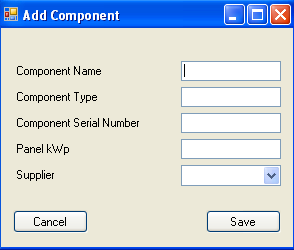
\includegraphics[scale=0.5]{frmAddComponent_scrot}
	\makeatletter
\def\PY@reset{\let\PY@it=\relax \let\PY@bf=\relax%
    \let\PY@ul=\relax \let\PY@tc=\relax%
    \let\PY@bc=\relax \let\PY@ff=\relax}
\def\PY@tok#1{\csname PY@tok@#1\endcsname}
\def\PY@toks#1+{\ifx\relax#1\empty\else%
    \PY@tok{#1}\expandafter\PY@toks\fi}
\def\PY@do#1{\PY@bc{\PY@tc{\PY@ul{%
    \PY@it{\PY@bf{\PY@ff{#1}}}}}}}
\def\PY#1#2{\PY@reset\PY@toks#1+\relax+\PY@do{#2}}

\expandafter\def\csname PY@tok@gd\endcsname{\def\PY@tc##1{\textcolor[rgb]{0.63,0.00,0.00}{##1}}}
\expandafter\def\csname PY@tok@gu\endcsname{\let\PY@bf=\textbf\def\PY@tc##1{\textcolor[rgb]{0.50,0.00,0.50}{##1}}}
\expandafter\def\csname PY@tok@gt\endcsname{\def\PY@tc##1{\textcolor[rgb]{0.00,0.25,0.82}{##1}}}
\expandafter\def\csname PY@tok@gs\endcsname{\let\PY@bf=\textbf}
\expandafter\def\csname PY@tok@gr\endcsname{\def\PY@tc##1{\textcolor[rgb]{1.00,0.00,0.00}{##1}}}
\expandafter\def\csname PY@tok@cm\endcsname{\let\PY@it=\textit\def\PY@tc##1{\textcolor[rgb]{0.25,0.50,0.50}{##1}}}
\expandafter\def\csname PY@tok@vg\endcsname{\def\PY@tc##1{\textcolor[rgb]{0.10,0.09,0.49}{##1}}}
\expandafter\def\csname PY@tok@m\endcsname{\def\PY@tc##1{\textcolor[rgb]{0.40,0.40,0.40}{##1}}}
\expandafter\def\csname PY@tok@mh\endcsname{\def\PY@tc##1{\textcolor[rgb]{0.40,0.40,0.40}{##1}}}
\expandafter\def\csname PY@tok@go\endcsname{\def\PY@tc##1{\textcolor[rgb]{0.50,0.50,0.50}{##1}}}
\expandafter\def\csname PY@tok@ge\endcsname{\let\PY@it=\textit}
\expandafter\def\csname PY@tok@vc\endcsname{\def\PY@tc##1{\textcolor[rgb]{0.10,0.09,0.49}{##1}}}
\expandafter\def\csname PY@tok@il\endcsname{\def\PY@tc##1{\textcolor[rgb]{0.40,0.40,0.40}{##1}}}
\expandafter\def\csname PY@tok@cs\endcsname{\let\PY@it=\textit\def\PY@tc##1{\textcolor[rgb]{0.25,0.50,0.50}{##1}}}
\expandafter\def\csname PY@tok@cp\endcsname{\def\PY@tc##1{\textcolor[rgb]{0.74,0.48,0.00}{##1}}}
\expandafter\def\csname PY@tok@gi\endcsname{\def\PY@tc##1{\textcolor[rgb]{0.00,0.63,0.00}{##1}}}
\expandafter\def\csname PY@tok@gh\endcsname{\let\PY@bf=\textbf\def\PY@tc##1{\textcolor[rgb]{0.00,0.00,0.50}{##1}}}
\expandafter\def\csname PY@tok@ni\endcsname{\let\PY@bf=\textbf\def\PY@tc##1{\textcolor[rgb]{0.60,0.60,0.60}{##1}}}
\expandafter\def\csname PY@tok@nl\endcsname{\def\PY@tc##1{\textcolor[rgb]{0.63,0.63,0.00}{##1}}}
\expandafter\def\csname PY@tok@nn\endcsname{\let\PY@bf=\textbf\def\PY@tc##1{\textcolor[rgb]{0.00,0.00,1.00}{##1}}}
\expandafter\def\csname PY@tok@no\endcsname{\def\PY@tc##1{\textcolor[rgb]{0.53,0.00,0.00}{##1}}}
\expandafter\def\csname PY@tok@na\endcsname{\def\PY@tc##1{\textcolor[rgb]{0.49,0.56,0.16}{##1}}}
\expandafter\def\csname PY@tok@nb\endcsname{\def\PY@tc##1{\textcolor[rgb]{0.00,0.50,0.00}{##1}}}
\expandafter\def\csname PY@tok@nc\endcsname{\let\PY@bf=\textbf\def\PY@tc##1{\textcolor[rgb]{0.00,0.00,1.00}{##1}}}
\expandafter\def\csname PY@tok@nd\endcsname{\def\PY@tc##1{\textcolor[rgb]{0.67,0.13,1.00}{##1}}}
\expandafter\def\csname PY@tok@ne\endcsname{\let\PY@bf=\textbf\def\PY@tc##1{\textcolor[rgb]{0.82,0.25,0.23}{##1}}}
\expandafter\def\csname PY@tok@nf\endcsname{\def\PY@tc##1{\textcolor[rgb]{0.00,0.00,1.00}{##1}}}
\expandafter\def\csname PY@tok@si\endcsname{\let\PY@bf=\textbf\def\PY@tc##1{\textcolor[rgb]{0.73,0.40,0.53}{##1}}}
\expandafter\def\csname PY@tok@s2\endcsname{\def\PY@tc##1{\textcolor[rgb]{0.73,0.13,0.13}{##1}}}
\expandafter\def\csname PY@tok@vi\endcsname{\def\PY@tc##1{\textcolor[rgb]{0.10,0.09,0.49}{##1}}}
\expandafter\def\csname PY@tok@nt\endcsname{\let\PY@bf=\textbf\def\PY@tc##1{\textcolor[rgb]{0.00,0.50,0.00}{##1}}}
\expandafter\def\csname PY@tok@nv\endcsname{\def\PY@tc##1{\textcolor[rgb]{0.10,0.09,0.49}{##1}}}
\expandafter\def\csname PY@tok@s1\endcsname{\def\PY@tc##1{\textcolor[rgb]{0.73,0.13,0.13}{##1}}}
\expandafter\def\csname PY@tok@sh\endcsname{\def\PY@tc##1{\textcolor[rgb]{0.73,0.13,0.13}{##1}}}
\expandafter\def\csname PY@tok@sc\endcsname{\def\PY@tc##1{\textcolor[rgb]{0.73,0.13,0.13}{##1}}}
\expandafter\def\csname PY@tok@sx\endcsname{\def\PY@tc##1{\textcolor[rgb]{0.00,0.50,0.00}{##1}}}
\expandafter\def\csname PY@tok@bp\endcsname{\def\PY@tc##1{\textcolor[rgb]{0.00,0.50,0.00}{##1}}}
\expandafter\def\csname PY@tok@c1\endcsname{\let\PY@it=\textit\def\PY@tc##1{\textcolor[rgb]{0.25,0.50,0.50}{##1}}}
\expandafter\def\csname PY@tok@kc\endcsname{\let\PY@bf=\textbf\def\PY@tc##1{\textcolor[rgb]{0.00,0.50,0.00}{##1}}}
\expandafter\def\csname PY@tok@c\endcsname{\let\PY@it=\textit\def\PY@tc##1{\textcolor[rgb]{0.25,0.50,0.50}{##1}}}
\expandafter\def\csname PY@tok@mf\endcsname{\def\PY@tc##1{\textcolor[rgb]{0.40,0.40,0.40}{##1}}}
\expandafter\def\csname PY@tok@err\endcsname{\def\PY@bc##1{\setlength{\fboxsep}{0pt}\fcolorbox[rgb]{1.00,0.00,0.00}{1,1,1}{\strut ##1}}}
\expandafter\def\csname PY@tok@kd\endcsname{\let\PY@bf=\textbf\def\PY@tc##1{\textcolor[rgb]{0.00,0.50,0.00}{##1}}}
\expandafter\def\csname PY@tok@ss\endcsname{\def\PY@tc##1{\textcolor[rgb]{0.10,0.09,0.49}{##1}}}
\expandafter\def\csname PY@tok@sr\endcsname{\def\PY@tc##1{\textcolor[rgb]{0.73,0.40,0.53}{##1}}}
\expandafter\def\csname PY@tok@mo\endcsname{\def\PY@tc##1{\textcolor[rgb]{0.40,0.40,0.40}{##1}}}
\expandafter\def\csname PY@tok@kn\endcsname{\let\PY@bf=\textbf\def\PY@tc##1{\textcolor[rgb]{0.00,0.50,0.00}{##1}}}
\expandafter\def\csname PY@tok@mi\endcsname{\def\PY@tc##1{\textcolor[rgb]{0.40,0.40,0.40}{##1}}}
\expandafter\def\csname PY@tok@gp\endcsname{\let\PY@bf=\textbf\def\PY@tc##1{\textcolor[rgb]{0.00,0.00,0.50}{##1}}}
\expandafter\def\csname PY@tok@o\endcsname{\def\PY@tc##1{\textcolor[rgb]{0.40,0.40,0.40}{##1}}}
\expandafter\def\csname PY@tok@kr\endcsname{\let\PY@bf=\textbf\def\PY@tc##1{\textcolor[rgb]{0.00,0.50,0.00}{##1}}}
\expandafter\def\csname PY@tok@s\endcsname{\def\PY@tc##1{\textcolor[rgb]{0.73,0.13,0.13}{##1}}}
\expandafter\def\csname PY@tok@kp\endcsname{\def\PY@tc##1{\textcolor[rgb]{0.00,0.50,0.00}{##1}}}
\expandafter\def\csname PY@tok@w\endcsname{\def\PY@tc##1{\textcolor[rgb]{0.73,0.73,0.73}{##1}}}
\expandafter\def\csname PY@tok@kt\endcsname{\def\PY@tc##1{\textcolor[rgb]{0.69,0.00,0.25}{##1}}}
\expandafter\def\csname PY@tok@ow\endcsname{\let\PY@bf=\textbf\def\PY@tc##1{\textcolor[rgb]{0.67,0.13,1.00}{##1}}}
\expandafter\def\csname PY@tok@sb\endcsname{\def\PY@tc##1{\textcolor[rgb]{0.73,0.13,0.13}{##1}}}
\expandafter\def\csname PY@tok@k\endcsname{\let\PY@bf=\textbf\def\PY@tc##1{\textcolor[rgb]{0.00,0.50,0.00}{##1}}}
\expandafter\def\csname PY@tok@se\endcsname{\let\PY@bf=\textbf\def\PY@tc##1{\textcolor[rgb]{0.73,0.40,0.13}{##1}}}
\expandafter\def\csname PY@tok@sd\endcsname{\let\PY@it=\textit\def\PY@tc##1{\textcolor[rgb]{0.73,0.13,0.13}{##1}}}

\def\PYZbs{\char`\\}
\def\PYZus{\char`\_}
\def\PYZob{\char`\{}
\def\PYZcb{\char`\}}
\def\PYZca{\char`\^}
\def\PYZam{\char`\&}
\def\PYZlt{\char`\<}
\def\PYZgt{\char`\>}
\def\PYZsh{\char`\#}
\def\PYZpc{\char`\%}
\def\PYZdl{\char`\$}
\def\PYZti{\char`\~}
% for compatibility with earlier versions
\def\PYZat{@}
\def\PYZlb{[}
\def\PYZrb{]}
\makeatother

\begin{Verbatim}[commandchars=\\\{\}]
\PY{err}{�}\PY{err}{�}\PY{err}{�}\PY{k}{Imports} \PY{n+nn}{System.Data}
\PY{k}{Imports} \PY{n+nn}{System.Data.OleDb}

\PY{k}{Class} \PY{n+nc}{frmAddComponent}
    \PY{c}{'THIS CODE SATISFIES SPECIFIC OBJECTIVE 5.}

    \PY{k}{Public} \PY{n}{accConnection} \PY{o+ow}{As} \PY{k}{New} \PY{n}{OleDbConnection}

    \PY{k}{Private} \PY{k}{Sub} \PY{n+nf}{AddComponent\PYZus{}Load}\PY{p}{(}\PY{k}{ByVal} \PY{n}{sender} \PY{o+ow}{As} \PY{n}{System}\PY{p}{.}\PY{n}{Object}\PY{p}{,} \PY{n}{\PYZus{}}
                                  \PY{k}{ByVal} \PY{n}{e} \PY{o+ow}{As} \PY{n}{System}\PY{p}{.}\PY{n}{EventArgs}\PY{p}{)} \PY{k}{Handles} \PY{k}{MyBase}\PY{p}{.}\PY{n}{Load}
        \PY{k}{If} \PY{n}{frmLoginForm}\PY{p}{.}\PY{n}{accConnection}\PY{p}{.}\PY{n}{State} \PY{o}{\PYZlt{}\PYZgt{}} \PY{n}{ConnectionState}\PY{p}{.}\PY{n}{Open} \PY{k}{Then}
            \PY{n}{frmLoginForm}\PY{p}{.}\PY{n}{accConnection}\PY{p}{.}\PY{n}{Open}\PY{p}{(}\PY{p}{)}
        \PY{k}{End} \PY{k}{If}

        \PY{n}{accConnection} \PY{o}{=} \PY{n}{frmLoginForm}\PY{p}{.}\PY{n}{accConnection}
        \PY{k}{Dim} \PY{n}{strSQL} \PY{o+ow}{As} \PY{k+kt}{String} \PY{o}{=} \PY{l+s}{"}\PY{l+s}{SELECT supp\PYZus{}name FROM Supplier}\PY{l+s}{"}
        \PY{k}{Dim} \PY{n}{da} \PY{o+ow}{As} \PY{k}{New} \PY{n}{OleDbDataAdapter}\PY{p}{(}\PY{n}{strSQL}\PY{p}{,} \PY{n}{accConnection}\PY{p}{)}
        \PY{k}{Dim} \PY{n}{ds} \PY{o+ow}{As} \PY{k}{New} \PY{n}{DataSet}

        \PY{n}{da}\PY{p}{.}\PY{n}{Fill}\PY{p}{(}\PY{n}{ds}\PY{p}{,} \PY{l+s}{"}\PY{l+s}{Supplier}\PY{l+s}{"}\PY{p}{)}

        \PY{k}{Dim} \PY{n}{dt} \PY{o+ow}{As} \PY{n}{DataTable} \PY{o}{=} \PY{n}{ds}\PY{p}{.}\PY{n}{Tables}\PY{p}{(}\PY{l+m+mi}{0}\PY{p}{)}
        \PY{k}{Dim} \PY{n}{dr} \PY{o+ow}{As} \PY{n}{DataRow}

        \PY{k}{For} \PY{k}{Each} \PY{n}{dr} \PY{o+ow}{In} \PY{n}{dt}\PY{p}{.}\PY{n}{Rows}\PY{p}{(}\PY{p}{)}
            \PY{c}{'List supplier names in the box so that the user can select}
            \PY{c}{'the supplier that the component is coming from.  Pull this}
            \PY{c}{'from the Supplier table.}
            \PY{n}{txtcbCompSupplierName}\PY{p}{.}\PY{n}{Items}\PY{p}{.}\PY{n}{Add}\PY{p}{(}\PY{n}{dr}\PY{p}{(}\PY{l+s}{"}\PY{l+s}{supp\PYZus{}name}\PY{l+s}{"}\PY{p}{)}\PY{p}{)}
        \PY{k}{Next}

        \PY{n}{txtcbCompSupplierName}\PY{p}{.}\PY{n}{SelectedIndex} \PY{o}{=} \PY{o}{-}\PY{l+m+mi}{1}

    \PY{k}{End} \PY{k}{Sub}

    \PY{k}{Private} \PY{k}{Sub} \PY{n+nf}{btnSave\PYZus{}Click}\PY{p}{(}\PY{k}{ByVal} \PY{n}{sender} \PY{o+ow}{As} \PY{n}{System}\PY{p}{.}\PY{n}{Object}\PY{p}{,} \PY{n}{\PYZus{}}
                              \PY{k}{ByVal} \PY{n}{e} \PY{o+ow}{As} \PY{n}{System}\PY{p}{.}\PY{n}{EventArgs}\PY{p}{)} \PY{k}{Handles} \PY{n}{btnSave}\PY{p}{.}\PY{n}{Click}

        \PY{c}{'This takes the supplier name from the supplier table and gets the}
        \PY{c}{'supplier ID from it, thereby letting it into the Component table.}

        \PY{k}{Dim} \PY{n}{suppidvaluecmd} \PY{o+ow}{As} \PY{k+kt}{String} \PY{o}{=} \PY{l+s}{"}\PY{l+s}{SELECT supp\PYZus{}id FROM Supplier WHERE }\PY{l+s}{"} \PY{n}{\PYZus{}}
                                       \PY{o}{\PYZam{}} \PY{l+s}{"}\PY{l+s}{supp\PYZus{}name = '}\PY{l+s}{"} \PY{o}{\PYZam{}} \PY{n}{txtcbCompSupplierName}\PY{p}{.}\PY{n}{SelectedItem} \PY{o}{\PYZam{}} \PY{l+s}{"}\PY{l+s}{'}\PY{l+s}{"}

        \PY{k}{Dim} \PY{n}{cmdString} \PY{o+ow}{As} \PY{k+kt}{String} \PY{o}{=} \PY{l+s}{"}\PY{l+s}{INSERT INTO Component (comp\PYZus{}name, comp\PYZus{}type, comp\PYZus{}serialno,}\PY{l+s}{"} \PY{n}{\PYZus{}}
                                  \PY{o}{\PYZam{}} \PY{l+s}{"}\PY{l+s}{ comp\PYZus{}panelwp, comp\PYZus{}supplier)}\PY{l+s}{"} \PY{n}{\PYZus{}}
                                  \PY{o}{\PYZam{}} \PY{l+s}{"}\PY{l+s}{VALUES (@comp\PYZus{}name,@comp\PYZus{}type,@comp\PYZus{}serialno,}\PY{l+s}{"} \PY{n}{\PYZus{}}
                                  \PY{o}{\PYZam{}} \PY{l+s}{"}\PY{l+s}{@comp\PYZus{}panelwp,@comp\PYZus{}supplier)}\PY{l+s}{"}

        \PY{k}{Dim} \PY{n}{da} \PY{o+ow}{As} \PY{k}{New} \PY{n}{OleDbDataAdapter}\PY{p}{(}\PY{n}{suppidvaluecmd}\PY{p}{,} \PY{n}{accConnection}\PY{p}{)}
        \PY{k}{Dim} \PY{n}{ds} \PY{o+ow}{As} \PY{k}{New} \PY{n}{DataSet}
        \PY{n}{da}\PY{p}{.}\PY{n}{Fill}\PY{p}{(}\PY{n}{ds}\PY{p}{,} \PY{l+s}{"}\PY{l+s}{Supplier}\PY{l+s}{"}\PY{p}{)}

        \PY{k}{Dim} \PY{n}{AddSupplierDataAdapter} \PY{o+ow}{As} \PY{k}{New} \PY{n}{OleDbDataAdapter}
        \PY{k}{Dim} \PY{n}{accCommand} \PY{o+ow}{As} \PY{k}{New} \PY{n}{OleDbCommand}
        \PY{k}{Dim} \PY{n}{intInsert} \PY{o+ow}{As} \PY{k+kt}{Integer}

        \PY{n}{accCommand}\PY{p}{.}\PY{n}{Connection} \PY{o}{=} \PY{n}{frmLoginForm}\PY{p}{.}\PY{n}{accConnection}
        \PY{n}{accCommand}\PY{p}{.}\PY{n}{CommandType} \PY{o}{=} \PY{n}{CommandType}\PY{p}{.}\PY{n}{Text}
        \PY{n}{accCommand}\PY{p}{.}\PY{n}{CommandText} \PY{o}{=} \PY{n}{cmdString}
        \PY{k}{Dim} \PY{n}{supplieridvalue} \PY{o+ow}{As} \PY{k+kt}{Integer} \PY{o}{=} \PY{n}{ds}\PY{p}{.}\PY{n}{Tables}\PY{p}{(}\PY{l+m+mi}{0}\PY{p}{)}\PY{p}{.}\PY{n}{Rows}\PY{p}{(}\PY{l+m+mi}{0}\PY{p}{)}\PY{p}{.}\PY{n}{Item}\PY{p}{(}\PY{l+s}{"}\PY{l+s}{supp\PYZus{}id}\PY{l+s}{"}\PY{p}{)}
        \PY{n}{MsgBox}\PY{p}{(}\PY{n}{supplieridvalue}\PY{p}{)}

        \PY{k}{Call} \PY{n}{InsertParameters}\PY{p}{(}\PY{n}{accCommand}\PY{p}{,} \PY{n}{supplieridvalue}\PY{p}{)}
        \PY{c}{'Now check if all the textboxes are populated.}
        \PY{k}{Try}
            \PY{n}{intInsert} \PY{o}{=} \PY{n}{accCommand}\PY{p}{.}\PY{n}{ExecuteNonQuery}\PY{p}{(}\PY{p}{)}
        \PY{k}{Catch} \PY{n}{ex} \PY{o+ow}{As} \PY{n}{Exception}
            \PY{n}{MsgBox}\PY{p}{(}\PY{l+s}{"}\PY{l+s}{Enter a value in each of the boxes, and make it a valid one!}\PY{l+s}{"}\PY{p}{)}
        \PY{k}{End} \PY{k}{Try}

        \PY{c}{'Call frmSwankyCode.CheckAdditions(intInsert, btnSave)}
    \PY{k}{End} \PY{k}{Sub}

    \PY{k}{Private} \PY{k}{Sub} \PY{n+nf}{InsertParameters}\PY{p}{(}\PY{k}{ByRef} \PY{n}{acccmd} \PY{o+ow}{As} \PY{n}{OleDbCommand}\PY{p}{,} \PY{k}{ByRef} \PY{n}{siv} \PY{o+ow}{As} \PY{k+kt}{Integer}\PY{p}{)}

        \PY{n}{acccmd}\PY{p}{.}\PY{n}{Parameters}\PY{p}{.}\PY{n}{Add}\PY{p}{(}\PY{l+s}{"}\PY{l+s}{@comp\PYZus{}name}\PY{l+s}{"}\PY{p}{,} \PY{n}{OleDbType}\PY{p}{.}\PY{n}{Char}\PY{p}{)}\PY{p}{.}\PY{n}{Value} \PY{o}{=} \PY{n}{txtComponentName}\PY{p}{.}\PY{n}{Text}
        \PY{n}{acccmd}\PY{p}{.}\PY{n}{Parameters}\PY{p}{.}\PY{n}{Add}\PY{p}{(}\PY{l+s}{"}\PY{l+s}{@comp\PYZus{}type}\PY{l+s}{"}\PY{p}{,} \PY{n}{OleDbType}\PY{p}{.}\PY{n}{Char}\PY{p}{)}\PY{p}{.}\PY{n}{Value} \PY{o}{=} \PY{n}{txtComponentType}\PY{p}{.}\PY{n}{Text}
        \PY{n}{acccmd}\PY{p}{.}\PY{n}{Parameters}\PY{p}{.}\PY{n}{Add}\PY{p}{(}\PY{l+s}{"}\PY{l+s}{@comp\PYZus{}serialno}\PY{l+s}{"}\PY{p}{,} \PY{n}{OleDbType}\PY{p}{.}\PY{n}{Char}\PY{p}{)}\PY{p}{.}\PY{n}{Value} \PY{o}{=} \PY{n}{txtComponentSerialNo}\PY{p}{.}\PY{n}{Text}
        \PY{c}{'Boundary data + erroneus data...}
        \PY{k}{Try}
            \PY{k}{If} \PY{n}{txtComponentPanelkWp}\PY{p}{.}\PY{n}{Text} \PY{o}{\PYZgt{}=} \PY{l+m+mi}{0} \PY{k}{Then}
                \PY{c}{'Multiply by 1000 to get the watt for the database rather than the}
                \PY{c}{'kilowatt value from the user.}
                \PY{n}{acccmd}\PY{p}{.}\PY{n}{Parameters}\PY{p}{.}\PY{n}{Add}\PY{p}{(}\PY{l+s}{"}\PY{l+s}{@comp\PYZus{}panelwp}\PY{l+s}{"}\PY{p}{,} \PY{n}{OleDbType}\PY{p}{.}\PY{n}{Numeric}\PY{p}{)}\PY{p}{.}\PY{n}{Value} \PY{o}{=} \PY{n}{txtComponentPanelkWp}\PY{p}{.}\PY{n}{Text} \PY{n}{\PYZus{}}
                                                                        \PY{o}{*} \PY{l+m+mi}{1000}
            \PY{k}{Else}
                \PY{n}{MsgBox}\PY{p}{(}\PY{l+s}{"}\PY{l+s}{The panel's kWp cannot be negative.}\PY{l+s}{"}\PY{p}{)}
            \PY{k}{End} \PY{k}{If}
            
        \PY{k}{Catch} \PY{n}{ex} \PY{o+ow}{As} \PY{n}{Exception}
            \PY{n}{MsgBox}\PY{p}{(}\PY{l+s}{"}\PY{l+s}{No numbers in the kWp box!}\PY{l+s}{"}\PY{p}{)}
        \PY{k}{End} \PY{k}{Try}
        \PY{c}{'And now the supplier ID value.}
        \PY{n}{acccmd}\PY{p}{.}\PY{n}{Parameters}\PY{p}{.}\PY{n}{Add}\PY{p}{(}\PY{l+s}{"}\PY{l+s}{@comp\PYZus{}supplier}\PY{l+s}{"}\PY{p}{,} \PY{n}{OleDbType}\PY{p}{.}\PY{n}{Numeric}\PY{p}{)}\PY{p}{.}\PY{n}{Value} \PY{o}{=} \PY{n}{siv}
    \PY{k}{End} \PY{k}{Sub}

    \PY{k}{Private} \PY{k}{Sub} \PY{n+nf}{btnCancel\PYZus{}Click}\PY{p}{(}\PY{k}{ByVal} \PY{n}{sender} \PY{o+ow}{As} \PY{n}{System}\PY{p}{.}\PY{n}{Object}\PY{p}{,} \PY{n}{\PYZus{}}
                                \PY{k}{ByVal} \PY{n}{e} \PY{o+ow}{As} \PY{n}{System}\PY{p}{.}\PY{n}{EventArgs}\PY{p}{)} \PY{k}{Handles} \PY{n}{btnCancel}\PY{p}{.}\PY{n}{Click}

        \PY{k}{If} \PY{n}{btnSave}\PY{p}{.}\PY{n}{Enabled} \PY{o}{=} \PY{k}{False} \PY{k}{Then}
            \PY{c}{'It's all fine and has gone through OK, so don't display a}
            \PY{c}{'message because that would just be annoying, just close this}
            \PY{c}{'and display the previous form.}
            \PY{k}{Me}\PY{p}{.}\PY{n}{Close}\PY{p}{(}\PY{p}{)}
            \PY{n}{frmAdd}\PY{p}{.}\PY{n}{Show}\PY{p}{(}\PY{p}{)}
        \PY{k}{Else}
            \PY{c}{'If it hasn't gone through OK, or nothing has been added,}
            \PY{c}{'then let the user know this so as not to panic them;}
            \PY{c}{'if the user did not mean to click the button, he/she knows.}
            \PY{n}{MsgBox}\PY{p}{(}\PY{l+s}{"}\PY{l+s}{This window will close and these details will not be saved.}\PY{l+s}{"}\PY{p}{)}
            \PY{k}{Me}\PY{p}{.}\PY{n}{Close}\PY{p}{(}\PY{p}{)}
            \PY{n}{frmAdd}\PY{p}{.}\PY{n}{Show}\PY{p}{(}\PY{p}{)}
        \PY{k}{End} \PY{k}{If}

    \PY{k}{End} \PY{k}{Sub}

\PY{k}{End} \PY{k}{Class}
\end{Verbatim}

\subsection{frmRemove}
	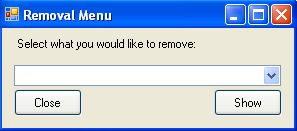
\includegraphics[scale=0.5]{frmRemove_scrot}
	\makeatletter
\def\PY@reset{\let\PY@it=\relax \let\PY@bf=\relax%
    \let\PY@ul=\relax \let\PY@tc=\relax%
    \let\PY@bc=\relax \let\PY@ff=\relax}
\def\PY@tok#1{\csname PY@tok@#1\endcsname}
\def\PY@toks#1+{\ifx\relax#1\empty\else%
    \PY@tok{#1}\expandafter\PY@toks\fi}
\def\PY@do#1{\PY@bc{\PY@tc{\PY@ul{%
    \PY@it{\PY@bf{\PY@ff{#1}}}}}}}
\def\PY#1#2{\PY@reset\PY@toks#1+\relax+\PY@do{#2}}

\expandafter\def\csname PY@tok@gd\endcsname{\def\PY@tc##1{\textcolor[rgb]{0.63,0.00,0.00}{##1}}}
\expandafter\def\csname PY@tok@gu\endcsname{\let\PY@bf=\textbf\def\PY@tc##1{\textcolor[rgb]{0.50,0.00,0.50}{##1}}}
\expandafter\def\csname PY@tok@gt\endcsname{\def\PY@tc##1{\textcolor[rgb]{0.00,0.25,0.82}{##1}}}
\expandafter\def\csname PY@tok@gs\endcsname{\let\PY@bf=\textbf}
\expandafter\def\csname PY@tok@gr\endcsname{\def\PY@tc##1{\textcolor[rgb]{1.00,0.00,0.00}{##1}}}
\expandafter\def\csname PY@tok@cm\endcsname{\let\PY@it=\textit\def\PY@tc##1{\textcolor[rgb]{0.25,0.50,0.50}{##1}}}
\expandafter\def\csname PY@tok@vg\endcsname{\def\PY@tc##1{\textcolor[rgb]{0.10,0.09,0.49}{##1}}}
\expandafter\def\csname PY@tok@m\endcsname{\def\PY@tc##1{\textcolor[rgb]{0.40,0.40,0.40}{##1}}}
\expandafter\def\csname PY@tok@mh\endcsname{\def\PY@tc##1{\textcolor[rgb]{0.40,0.40,0.40}{##1}}}
\expandafter\def\csname PY@tok@go\endcsname{\def\PY@tc##1{\textcolor[rgb]{0.50,0.50,0.50}{##1}}}
\expandafter\def\csname PY@tok@ge\endcsname{\let\PY@it=\textit}
\expandafter\def\csname PY@tok@vc\endcsname{\def\PY@tc##1{\textcolor[rgb]{0.10,0.09,0.49}{##1}}}
\expandafter\def\csname PY@tok@il\endcsname{\def\PY@tc##1{\textcolor[rgb]{0.40,0.40,0.40}{##1}}}
\expandafter\def\csname PY@tok@cs\endcsname{\let\PY@it=\textit\def\PY@tc##1{\textcolor[rgb]{0.25,0.50,0.50}{##1}}}
\expandafter\def\csname PY@tok@cp\endcsname{\def\PY@tc##1{\textcolor[rgb]{0.74,0.48,0.00}{##1}}}
\expandafter\def\csname PY@tok@gi\endcsname{\def\PY@tc##1{\textcolor[rgb]{0.00,0.63,0.00}{##1}}}
\expandafter\def\csname PY@tok@gh\endcsname{\let\PY@bf=\textbf\def\PY@tc##1{\textcolor[rgb]{0.00,0.00,0.50}{##1}}}
\expandafter\def\csname PY@tok@ni\endcsname{\let\PY@bf=\textbf\def\PY@tc##1{\textcolor[rgb]{0.60,0.60,0.60}{##1}}}
\expandafter\def\csname PY@tok@nl\endcsname{\def\PY@tc##1{\textcolor[rgb]{0.63,0.63,0.00}{##1}}}
\expandafter\def\csname PY@tok@nn\endcsname{\let\PY@bf=\textbf\def\PY@tc##1{\textcolor[rgb]{0.00,0.00,1.00}{##1}}}
\expandafter\def\csname PY@tok@no\endcsname{\def\PY@tc##1{\textcolor[rgb]{0.53,0.00,0.00}{##1}}}
\expandafter\def\csname PY@tok@na\endcsname{\def\PY@tc##1{\textcolor[rgb]{0.49,0.56,0.16}{##1}}}
\expandafter\def\csname PY@tok@nb\endcsname{\def\PY@tc##1{\textcolor[rgb]{0.00,0.50,0.00}{##1}}}
\expandafter\def\csname PY@tok@nc\endcsname{\let\PY@bf=\textbf\def\PY@tc##1{\textcolor[rgb]{0.00,0.00,1.00}{##1}}}
\expandafter\def\csname PY@tok@nd\endcsname{\def\PY@tc##1{\textcolor[rgb]{0.67,0.13,1.00}{##1}}}
\expandafter\def\csname PY@tok@ne\endcsname{\let\PY@bf=\textbf\def\PY@tc##1{\textcolor[rgb]{0.82,0.25,0.23}{##1}}}
\expandafter\def\csname PY@tok@nf\endcsname{\def\PY@tc##1{\textcolor[rgb]{0.00,0.00,1.00}{##1}}}
\expandafter\def\csname PY@tok@si\endcsname{\let\PY@bf=\textbf\def\PY@tc##1{\textcolor[rgb]{0.73,0.40,0.53}{##1}}}
\expandafter\def\csname PY@tok@s2\endcsname{\def\PY@tc##1{\textcolor[rgb]{0.73,0.13,0.13}{##1}}}
\expandafter\def\csname PY@tok@vi\endcsname{\def\PY@tc##1{\textcolor[rgb]{0.10,0.09,0.49}{##1}}}
\expandafter\def\csname PY@tok@nt\endcsname{\let\PY@bf=\textbf\def\PY@tc##1{\textcolor[rgb]{0.00,0.50,0.00}{##1}}}
\expandafter\def\csname PY@tok@nv\endcsname{\def\PY@tc##1{\textcolor[rgb]{0.10,0.09,0.49}{##1}}}
\expandafter\def\csname PY@tok@s1\endcsname{\def\PY@tc##1{\textcolor[rgb]{0.73,0.13,0.13}{##1}}}
\expandafter\def\csname PY@tok@sh\endcsname{\def\PY@tc##1{\textcolor[rgb]{0.73,0.13,0.13}{##1}}}
\expandafter\def\csname PY@tok@sc\endcsname{\def\PY@tc##1{\textcolor[rgb]{0.73,0.13,0.13}{##1}}}
\expandafter\def\csname PY@tok@sx\endcsname{\def\PY@tc##1{\textcolor[rgb]{0.00,0.50,0.00}{##1}}}
\expandafter\def\csname PY@tok@bp\endcsname{\def\PY@tc##1{\textcolor[rgb]{0.00,0.50,0.00}{##1}}}
\expandafter\def\csname PY@tok@c1\endcsname{\let\PY@it=\textit\def\PY@tc##1{\textcolor[rgb]{0.25,0.50,0.50}{##1}}}
\expandafter\def\csname PY@tok@kc\endcsname{\let\PY@bf=\textbf\def\PY@tc##1{\textcolor[rgb]{0.00,0.50,0.00}{##1}}}
\expandafter\def\csname PY@tok@c\endcsname{\let\PY@it=\textit\def\PY@tc##1{\textcolor[rgb]{0.25,0.50,0.50}{##1}}}
\expandafter\def\csname PY@tok@mf\endcsname{\def\PY@tc##1{\textcolor[rgb]{0.40,0.40,0.40}{##1}}}
\expandafter\def\csname PY@tok@err\endcsname{\def\PY@bc##1{\setlength{\fboxsep}{0pt}\fcolorbox[rgb]{1.00,0.00,0.00}{1,1,1}{\strut ##1}}}
\expandafter\def\csname PY@tok@kd\endcsname{\let\PY@bf=\textbf\def\PY@tc##1{\textcolor[rgb]{0.00,0.50,0.00}{##1}}}
\expandafter\def\csname PY@tok@ss\endcsname{\def\PY@tc##1{\textcolor[rgb]{0.10,0.09,0.49}{##1}}}
\expandafter\def\csname PY@tok@sr\endcsname{\def\PY@tc##1{\textcolor[rgb]{0.73,0.40,0.53}{##1}}}
\expandafter\def\csname PY@tok@mo\endcsname{\def\PY@tc##1{\textcolor[rgb]{0.40,0.40,0.40}{##1}}}
\expandafter\def\csname PY@tok@kn\endcsname{\let\PY@bf=\textbf\def\PY@tc##1{\textcolor[rgb]{0.00,0.50,0.00}{##1}}}
\expandafter\def\csname PY@tok@mi\endcsname{\def\PY@tc##1{\textcolor[rgb]{0.40,0.40,0.40}{##1}}}
\expandafter\def\csname PY@tok@gp\endcsname{\let\PY@bf=\textbf\def\PY@tc##1{\textcolor[rgb]{0.00,0.00,0.50}{##1}}}
\expandafter\def\csname PY@tok@o\endcsname{\def\PY@tc##1{\textcolor[rgb]{0.40,0.40,0.40}{##1}}}
\expandafter\def\csname PY@tok@kr\endcsname{\let\PY@bf=\textbf\def\PY@tc##1{\textcolor[rgb]{0.00,0.50,0.00}{##1}}}
\expandafter\def\csname PY@tok@s\endcsname{\def\PY@tc##1{\textcolor[rgb]{0.73,0.13,0.13}{##1}}}
\expandafter\def\csname PY@tok@kp\endcsname{\def\PY@tc##1{\textcolor[rgb]{0.00,0.50,0.00}{##1}}}
\expandafter\def\csname PY@tok@w\endcsname{\def\PY@tc##1{\textcolor[rgb]{0.73,0.73,0.73}{##1}}}
\expandafter\def\csname PY@tok@kt\endcsname{\def\PY@tc##1{\textcolor[rgb]{0.69,0.00,0.25}{##1}}}
\expandafter\def\csname PY@tok@ow\endcsname{\let\PY@bf=\textbf\def\PY@tc##1{\textcolor[rgb]{0.67,0.13,1.00}{##1}}}
\expandafter\def\csname PY@tok@sb\endcsname{\def\PY@tc##1{\textcolor[rgb]{0.73,0.13,0.13}{##1}}}
\expandafter\def\csname PY@tok@k\endcsname{\let\PY@bf=\textbf\def\PY@tc##1{\textcolor[rgb]{0.00,0.50,0.00}{##1}}}
\expandafter\def\csname PY@tok@se\endcsname{\let\PY@bf=\textbf\def\PY@tc##1{\textcolor[rgb]{0.73,0.40,0.13}{##1}}}
\expandafter\def\csname PY@tok@sd\endcsname{\let\PY@it=\textit\def\PY@tc##1{\textcolor[rgb]{0.73,0.13,0.13}{##1}}}

\def\PYZbs{\char`\\}
\def\PYZus{\char`\_}
\def\PYZob{\char`\{}
\def\PYZcb{\char`\}}
\def\PYZca{\char`\^}
\def\PYZam{\char`\&}
\def\PYZlt{\char`\<}
\def\PYZgt{\char`\>}
\def\PYZsh{\char`\#}
\def\PYZpc{\char`\%}
\def\PYZdl{\char`\$}
\def\PYZti{\char`\~}
% for compatibility with earlier versions
\def\PYZat{@}
\def\PYZlb{[}
\def\PYZrb{]}
\makeatother

\begin{Verbatim}[commandchars=\\\{\}]
\PY{err}{�}\PY{err}{�}\PY{err}{�}\PY{k}{Public} \PY{k}{Class} \PY{n+nc}{frmRemove}

    \PY{k}{Private} \PY{k}{Sub} \PY{n+nf}{frmRemove\PYZus{}Load}\PY{p}{(}\PY{k}{ByVal} \PY{n}{sender} \PY{o+ow}{As} \PY{n}{System}\PY{p}{.}\PY{n}{Object}\PY{p}{,} \PY{n}{\PYZus{}}
                               \PY{k}{ByVal} \PY{n}{e} \PY{o+ow}{As} \PY{n}{System}\PY{p}{.}\PY{n}{EventArgs}\PY{p}{)} \PY{k}{Handles} \PY{k}{MyBase}\PY{p}{.}\PY{n}{Load}
        \PY{c}{'Check if the database connection is breathing.}
        \PY{c}{'If it isn't, resuscitate it.  :-)}
        \PY{k}{If} \PY{n}{frmLoginForm}\PY{p}{.}\PY{n}{accConnection}\PY{p}{.}\PY{n}{State} \PY{o}{\PYZlt{}\PYZgt{}} \PY{n}{ConnectionState}\PY{p}{.}\PY{n}{Open} \PY{k}{Then}
            \PY{n}{frmLoginForm}\PY{p}{.}\PY{n}{accConnection}\PY{p}{.}\PY{n}{Open}\PY{p}{(}\PY{p}{)}
        \PY{k}{End} \PY{k}{If}

        \PY{n}{cbtxtRemoveOptions}\PY{p}{.}\PY{n}{Items}\PY{p}{.}\PY{n}{Add}\PY{p}{(}\PY{l+s}{"}\PY{l+s}{Customer}\PY{l+s}{"}\PY{p}{)}
        \PY{n}{cbtxtRemoveOptions}\PY{p}{.}\PY{n}{Items}\PY{p}{.}\PY{n}{Add}\PY{p}{(}\PY{l+s}{"}\PY{l+s}{Supplier}\PY{l+s}{"}\PY{p}{)}
        \PY{n}{cbtxtRemoveOptions}\PY{p}{.}\PY{n}{Items}\PY{p}{.}\PY{n}{Add}\PY{p}{(}\PY{l+s}{"}\PY{l+s}{Component}\PY{l+s}{"}\PY{p}{)}
    \PY{k}{End} \PY{k}{Sub}

    \PY{k}{Private} \PY{k}{Sub} \PY{n+nf}{btnShow\PYZus{}Click}\PY{p}{(}\PY{k}{ByVal} \PY{n}{sender} \PY{o+ow}{As} \PY{n}{System}\PY{p}{.}\PY{n}{Object}\PY{p}{,} \PY{n}{\PYZus{}}
                              \PY{k}{ByVal} \PY{n}{e} \PY{o+ow}{As} \PY{n}{System}\PY{p}{.}\PY{n}{EventArgs}\PY{p}{)} \PY{k}{Handles} \PY{n}{btnShow}\PY{p}{.}\PY{n}{Click}

        \PY{c}{'According to the option selected, display the next form and hide}
        \PY{c}{'this one.}
        \PY{k}{If} \PY{n}{cbtxtRemoveOptions}\PY{p}{.}\PY{n}{Text} \PY{o}{=} \PY{l+s}{"}\PY{l+s}{Customer}\PY{l+s}{"} \PY{k}{Then}
            \PY{k}{Me}\PY{p}{.}\PY{n}{Hide}\PY{p}{(}\PY{p}{)}
            \PY{n}{frmRemoveCustomer}\PY{p}{.}\PY{n}{Show}\PY{p}{(}\PY{p}{)}
        \PY{k}{ElseIf} \PY{n}{cbtxtRemoveOptions}\PY{p}{.}\PY{n}{Text} \PY{o}{=} \PY{l+s}{"}\PY{l+s}{Supplier}\PY{l+s}{"} \PY{k}{Then}
            \PY{k}{Me}\PY{p}{.}\PY{n}{Hide}\PY{p}{(}\PY{p}{)}
            \PY{n}{frmRemoveSupplier}\PY{p}{.}\PY{n}{Show}\PY{p}{(}\PY{p}{)}
        \PY{k}{ElseIf} \PY{n}{cbtxtRemoveOptions}\PY{p}{.}\PY{n}{Text} \PY{o}{=} \PY{l+s}{"}\PY{l+s}{Component}\PY{l+s}{"} \PY{k}{Then}
            \PY{k}{Me}\PY{p}{.}\PY{n}{Hide}\PY{p}{(}\PY{p}{)}
            \PY{n}{frmRemoveComponent}\PY{p}{.}\PY{n}{Show}\PY{p}{(}\PY{p}{)}
        \PY{k}{End} \PY{k}{If}

    \PY{k}{End} \PY{k}{Sub}

    \PY{k}{Private} \PY{k}{Sub} \PY{n+nf}{btnClose\PYZus{}Click}\PY{p}{(}\PY{k}{ByVal} \PY{n}{sender} \PY{o+ow}{As} \PY{n}{System}\PY{p}{.}\PY{n}{Object}\PY{p}{,} \PY{n}{\PYZus{}}
                               \PY{k}{ByVal} \PY{n}{e} \PY{o+ow}{As} \PY{n}{System}\PY{p}{.}\PY{n}{EventArgs}\PY{p}{)} \PY{k}{Handles} \PY{n}{btnClose}\PY{p}{.}\PY{n}{Click}
        \PY{c}{'Close this window and show the main menu.}
        \PY{k}{Me}\PY{p}{.}\PY{n}{Close}\PY{p}{(}\PY{p}{)}
        \PY{n}{frmMainMenu}\PY{p}{.}\PY{n}{Show}\PY{p}{(}\PY{p}{)}
    \PY{k}{End} \PY{k}{Sub}
\PY{k}{End} \PY{k}{Class}
\end{Verbatim}

	
\subsection{frmRemoveCustomer}
	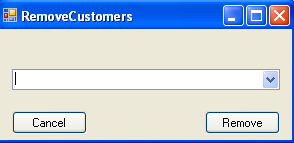
\includegraphics[scale=0.5]{frmRemoveCustomer_scrot}
	\makeatletter
\def\PY@reset{\let\PY@it=\relax \let\PY@bf=\relax%
    \let\PY@ul=\relax \let\PY@tc=\relax%
    \let\PY@bc=\relax \let\PY@ff=\relax}
\def\PY@tok#1{\csname PY@tok@#1\endcsname}
\def\PY@toks#1+{\ifx\relax#1\empty\else%
    \PY@tok{#1}\expandafter\PY@toks\fi}
\def\PY@do#1{\PY@bc{\PY@tc{\PY@ul{%
    \PY@it{\PY@bf{\PY@ff{#1}}}}}}}
\def\PY#1#2{\PY@reset\PY@toks#1+\relax+\PY@do{#2}}

\expandafter\def\csname PY@tok@gd\endcsname{\def\PY@tc##1{\textcolor[rgb]{0.63,0.00,0.00}{##1}}}
\expandafter\def\csname PY@tok@gu\endcsname{\let\PY@bf=\textbf\def\PY@tc##1{\textcolor[rgb]{0.50,0.00,0.50}{##1}}}
\expandafter\def\csname PY@tok@gt\endcsname{\def\PY@tc##1{\textcolor[rgb]{0.00,0.25,0.82}{##1}}}
\expandafter\def\csname PY@tok@gs\endcsname{\let\PY@bf=\textbf}
\expandafter\def\csname PY@tok@gr\endcsname{\def\PY@tc##1{\textcolor[rgb]{1.00,0.00,0.00}{##1}}}
\expandafter\def\csname PY@tok@cm\endcsname{\let\PY@it=\textit\def\PY@tc##1{\textcolor[rgb]{0.25,0.50,0.50}{##1}}}
\expandafter\def\csname PY@tok@vg\endcsname{\def\PY@tc##1{\textcolor[rgb]{0.10,0.09,0.49}{##1}}}
\expandafter\def\csname PY@tok@m\endcsname{\def\PY@tc##1{\textcolor[rgb]{0.40,0.40,0.40}{##1}}}
\expandafter\def\csname PY@tok@mh\endcsname{\def\PY@tc##1{\textcolor[rgb]{0.40,0.40,0.40}{##1}}}
\expandafter\def\csname PY@tok@go\endcsname{\def\PY@tc##1{\textcolor[rgb]{0.50,0.50,0.50}{##1}}}
\expandafter\def\csname PY@tok@ge\endcsname{\let\PY@it=\textit}
\expandafter\def\csname PY@tok@vc\endcsname{\def\PY@tc##1{\textcolor[rgb]{0.10,0.09,0.49}{##1}}}
\expandafter\def\csname PY@tok@il\endcsname{\def\PY@tc##1{\textcolor[rgb]{0.40,0.40,0.40}{##1}}}
\expandafter\def\csname PY@tok@cs\endcsname{\let\PY@it=\textit\def\PY@tc##1{\textcolor[rgb]{0.25,0.50,0.50}{##1}}}
\expandafter\def\csname PY@tok@cp\endcsname{\def\PY@tc##1{\textcolor[rgb]{0.74,0.48,0.00}{##1}}}
\expandafter\def\csname PY@tok@gi\endcsname{\def\PY@tc##1{\textcolor[rgb]{0.00,0.63,0.00}{##1}}}
\expandafter\def\csname PY@tok@gh\endcsname{\let\PY@bf=\textbf\def\PY@tc##1{\textcolor[rgb]{0.00,0.00,0.50}{##1}}}
\expandafter\def\csname PY@tok@ni\endcsname{\let\PY@bf=\textbf\def\PY@tc##1{\textcolor[rgb]{0.60,0.60,0.60}{##1}}}
\expandafter\def\csname PY@tok@nl\endcsname{\def\PY@tc##1{\textcolor[rgb]{0.63,0.63,0.00}{##1}}}
\expandafter\def\csname PY@tok@nn\endcsname{\let\PY@bf=\textbf\def\PY@tc##1{\textcolor[rgb]{0.00,0.00,1.00}{##1}}}
\expandafter\def\csname PY@tok@no\endcsname{\def\PY@tc##1{\textcolor[rgb]{0.53,0.00,0.00}{##1}}}
\expandafter\def\csname PY@tok@na\endcsname{\def\PY@tc##1{\textcolor[rgb]{0.49,0.56,0.16}{##1}}}
\expandafter\def\csname PY@tok@nb\endcsname{\def\PY@tc##1{\textcolor[rgb]{0.00,0.50,0.00}{##1}}}
\expandafter\def\csname PY@tok@nc\endcsname{\let\PY@bf=\textbf\def\PY@tc##1{\textcolor[rgb]{0.00,0.00,1.00}{##1}}}
\expandafter\def\csname PY@tok@nd\endcsname{\def\PY@tc##1{\textcolor[rgb]{0.67,0.13,1.00}{##1}}}
\expandafter\def\csname PY@tok@ne\endcsname{\let\PY@bf=\textbf\def\PY@tc##1{\textcolor[rgb]{0.82,0.25,0.23}{##1}}}
\expandafter\def\csname PY@tok@nf\endcsname{\def\PY@tc##1{\textcolor[rgb]{0.00,0.00,1.00}{##1}}}
\expandafter\def\csname PY@tok@si\endcsname{\let\PY@bf=\textbf\def\PY@tc##1{\textcolor[rgb]{0.73,0.40,0.53}{##1}}}
\expandafter\def\csname PY@tok@s2\endcsname{\def\PY@tc##1{\textcolor[rgb]{0.73,0.13,0.13}{##1}}}
\expandafter\def\csname PY@tok@vi\endcsname{\def\PY@tc##1{\textcolor[rgb]{0.10,0.09,0.49}{##1}}}
\expandafter\def\csname PY@tok@nt\endcsname{\let\PY@bf=\textbf\def\PY@tc##1{\textcolor[rgb]{0.00,0.50,0.00}{##1}}}
\expandafter\def\csname PY@tok@nv\endcsname{\def\PY@tc##1{\textcolor[rgb]{0.10,0.09,0.49}{##1}}}
\expandafter\def\csname PY@tok@s1\endcsname{\def\PY@tc##1{\textcolor[rgb]{0.73,0.13,0.13}{##1}}}
\expandafter\def\csname PY@tok@sh\endcsname{\def\PY@tc##1{\textcolor[rgb]{0.73,0.13,0.13}{##1}}}
\expandafter\def\csname PY@tok@sc\endcsname{\def\PY@tc##1{\textcolor[rgb]{0.73,0.13,0.13}{##1}}}
\expandafter\def\csname PY@tok@sx\endcsname{\def\PY@tc##1{\textcolor[rgb]{0.00,0.50,0.00}{##1}}}
\expandafter\def\csname PY@tok@bp\endcsname{\def\PY@tc##1{\textcolor[rgb]{0.00,0.50,0.00}{##1}}}
\expandafter\def\csname PY@tok@c1\endcsname{\let\PY@it=\textit\def\PY@tc##1{\textcolor[rgb]{0.25,0.50,0.50}{##1}}}
\expandafter\def\csname PY@tok@kc\endcsname{\let\PY@bf=\textbf\def\PY@tc##1{\textcolor[rgb]{0.00,0.50,0.00}{##1}}}
\expandafter\def\csname PY@tok@c\endcsname{\let\PY@it=\textit\def\PY@tc##1{\textcolor[rgb]{0.25,0.50,0.50}{##1}}}
\expandafter\def\csname PY@tok@mf\endcsname{\def\PY@tc##1{\textcolor[rgb]{0.40,0.40,0.40}{##1}}}
\expandafter\def\csname PY@tok@err\endcsname{\def\PY@bc##1{\setlength{\fboxsep}{0pt}\fcolorbox[rgb]{1.00,0.00,0.00}{1,1,1}{\strut ##1}}}
\expandafter\def\csname PY@tok@kd\endcsname{\let\PY@bf=\textbf\def\PY@tc##1{\textcolor[rgb]{0.00,0.50,0.00}{##1}}}
\expandafter\def\csname PY@tok@ss\endcsname{\def\PY@tc##1{\textcolor[rgb]{0.10,0.09,0.49}{##1}}}
\expandafter\def\csname PY@tok@sr\endcsname{\def\PY@tc##1{\textcolor[rgb]{0.73,0.40,0.53}{##1}}}
\expandafter\def\csname PY@tok@mo\endcsname{\def\PY@tc##1{\textcolor[rgb]{0.40,0.40,0.40}{##1}}}
\expandafter\def\csname PY@tok@kn\endcsname{\let\PY@bf=\textbf\def\PY@tc##1{\textcolor[rgb]{0.00,0.50,0.00}{##1}}}
\expandafter\def\csname PY@tok@mi\endcsname{\def\PY@tc##1{\textcolor[rgb]{0.40,0.40,0.40}{##1}}}
\expandafter\def\csname PY@tok@gp\endcsname{\let\PY@bf=\textbf\def\PY@tc##1{\textcolor[rgb]{0.00,0.00,0.50}{##1}}}
\expandafter\def\csname PY@tok@o\endcsname{\def\PY@tc##1{\textcolor[rgb]{0.40,0.40,0.40}{##1}}}
\expandafter\def\csname PY@tok@kr\endcsname{\let\PY@bf=\textbf\def\PY@tc##1{\textcolor[rgb]{0.00,0.50,0.00}{##1}}}
\expandafter\def\csname PY@tok@s\endcsname{\def\PY@tc##1{\textcolor[rgb]{0.73,0.13,0.13}{##1}}}
\expandafter\def\csname PY@tok@kp\endcsname{\def\PY@tc##1{\textcolor[rgb]{0.00,0.50,0.00}{##1}}}
\expandafter\def\csname PY@tok@w\endcsname{\def\PY@tc##1{\textcolor[rgb]{0.73,0.73,0.73}{##1}}}
\expandafter\def\csname PY@tok@kt\endcsname{\def\PY@tc##1{\textcolor[rgb]{0.69,0.00,0.25}{##1}}}
\expandafter\def\csname PY@tok@ow\endcsname{\let\PY@bf=\textbf\def\PY@tc##1{\textcolor[rgb]{0.67,0.13,1.00}{##1}}}
\expandafter\def\csname PY@tok@sb\endcsname{\def\PY@tc##1{\textcolor[rgb]{0.73,0.13,0.13}{##1}}}
\expandafter\def\csname PY@tok@k\endcsname{\let\PY@bf=\textbf\def\PY@tc##1{\textcolor[rgb]{0.00,0.50,0.00}{##1}}}
\expandafter\def\csname PY@tok@se\endcsname{\let\PY@bf=\textbf\def\PY@tc##1{\textcolor[rgb]{0.73,0.40,0.13}{##1}}}
\expandafter\def\csname PY@tok@sd\endcsname{\let\PY@it=\textit\def\PY@tc##1{\textcolor[rgb]{0.73,0.13,0.13}{##1}}}

\def\PYZbs{\char`\\}
\def\PYZus{\char`\_}
\def\PYZob{\char`\{}
\def\PYZcb{\char`\}}
\def\PYZca{\char`\^}
\def\PYZam{\char`\&}
\def\PYZlt{\char`\<}
\def\PYZgt{\char`\>}
\def\PYZsh{\char`\#}
\def\PYZpc{\char`\%}
\def\PYZdl{\char`\$}
\def\PYZti{\char`\~}
% for compatibility with earlier versions
\def\PYZat{@}
\def\PYZlb{[}
\def\PYZrb{]}
\makeatother

\begin{Verbatim}[commandchars=\\\{\}]
\PY{err}{�}\PY{err}{�}\PY{err}{�}\PY{k}{Imports} \PY{n+nn}{System.Data}
\PY{k}{Imports} \PY{n+nn}{System.Data.OleDb}

\PY{k}{Public} \PY{k}{Class} \PY{n+nc}{frmRemoveCustomer}
    \PY{c}{'THIS CODE SATISFIES SPECIFIC OBJECTIVE 6.}
    \PY{k}{Public} \PY{n}{accConnection} \PY{o+ow}{As} \PY{k}{New} \PY{n}{OleDbConnection}

    \PY{k}{Private} \PY{k}{Sub} \PY{n+nf}{frmRemoveCustomers\PYZus{}Load}\PY{p}{(}\PY{k}{ByVal} \PY{n}{sender} \PY{o+ow}{As} \PY{n}{System}\PY{p}{.}\PY{n}{Object}\PY{p}{,} \PY{n}{\PYZus{}}
                                        \PY{k}{ByVal} \PY{n}{e} \PY{o+ow}{As} \PY{n}{System}\PY{p}{.}\PY{n}{EventArgs}\PY{p}{)} \PY{k}{Handles} \PY{k}{MyBase}\PY{p}{.}\PY{n}{Load}
        \PY{k}{If} \PY{n}{frmLoginForm}\PY{p}{.}\PY{n}{accConnection}\PY{p}{.}\PY{n}{State} \PY{o}{\PYZlt{}\PYZgt{}} \PY{n}{ConnectionState}\PY{p}{.}\PY{n}{Open} \PY{k}{Then}
            \PY{n}{frmLoginForm}\PY{p}{.}\PY{n}{accConnection}\PY{p}{.}\PY{n}{Open}\PY{p}{(}\PY{p}{)}
        \PY{k}{End} \PY{k}{If}

        \PY{n}{accConnection} \PY{o}{=} \PY{n}{frmLoginForm}\PY{p}{.}\PY{n}{accConnection}
        \PY{k}{Dim} \PY{n}{strSQL} \PY{o+ow}{As} \PY{k+kt}{String} \PY{o}{=} \PY{l+s}{"}\PY{l+s}{SELECT cust\PYZus{}name FROM Customer}\PY{l+s}{"}
        \PY{k}{Dim} \PY{n}{da} \PY{o+ow}{As} \PY{k}{New} \PY{n}{OleDbDataAdapter}\PY{p}{(}\PY{n}{strSQL}\PY{p}{,} \PY{n}{accConnection}\PY{p}{)}
        \PY{k}{Dim} \PY{n}{ds} \PY{o+ow}{As} \PY{k}{New} \PY{n}{DataSet}

        \PY{n}{da}\PY{p}{.}\PY{n}{Fill}\PY{p}{(}\PY{n}{ds}\PY{p}{,} \PY{l+s}{"}\PY{l+s}{Customer}\PY{l+s}{"}\PY{p}{)}

        \PY{k}{Dim} \PY{n}{dt} \PY{o+ow}{As} \PY{n}{DataTable} \PY{o}{=} \PY{n}{ds}\PY{p}{.}\PY{n}{Tables}\PY{p}{(}\PY{l+m+mi}{0}\PY{p}{)}
        \PY{k}{Dim} \PY{n}{dr} \PY{o+ow}{As} \PY{n}{DataRow}

        \PY{k}{For} \PY{k}{Each} \PY{n}{dr} \PY{o+ow}{In} \PY{n}{dt}\PY{p}{.}\PY{n}{Rows}\PY{p}{(}\PY{p}{)}
            \PY{n}{txtcbCustomerRemove}\PY{p}{.}\PY{n}{Items}\PY{p}{.}\PY{n}{Add}\PY{p}{(}\PY{n}{dr}\PY{p}{(}\PY{l+s}{"}\PY{l+s}{cust\PYZus{}name}\PY{l+s}{"}\PY{p}{)}\PY{p}{)}
        \PY{k}{Next}

        \PY{n}{txtcbCustomerRemove}\PY{p}{.}\PY{n}{SelectedIndex} \PY{o}{=} \PY{o}{-}\PY{l+m+mi}{1}
    \PY{k}{End} \PY{k}{Sub}

    \PY{k}{Private} \PY{k}{Sub} \PY{n+nf}{btnRemove\PYZus{}Click}\PY{p}{(}\PY{k}{ByVal} \PY{n}{sender} \PY{o+ow}{As} \PY{n}{System}\PY{p}{.}\PY{n}{Object}\PY{p}{,} \PY{n}{\PYZus{}}
                                \PY{k}{ByVal} \PY{n}{e} \PY{o+ow}{As} \PY{n}{System}\PY{p}{.}\PY{n}{EventArgs}\PY{p}{)} \PY{k}{Handles} \PY{n}{btnRemove}\PY{p}{.}\PY{n}{Click}

        \PY{k}{Dim} \PY{n}{cmdString} \PY{o+ow}{As} \PY{k+kt}{String} \PY{o}{=} \PY{l+s}{"}\PY{l+s}{DELETE * FROM Customer WHERE cust\PYZus{}name = '}\PY{l+s}{"} \PY{o}{\PYZam{}} \PY{n}{\PYZus{}}
                                    \PY{k}{Me}\PY{p}{.}\PY{n}{txtcbCustomerRemove}\PY{p}{.}\PY{n}{SelectedItem} \PY{o}{\PYZam{}} \PY{l+s}{"}\PY{l+s}{'}\PY{l+s}{"}
        \PY{k}{Dim} \PY{n}{da} \PY{o+ow}{As} \PY{k}{New} \PY{n}{OleDbDataAdapter}\PY{p}{(}\PY{n}{cmdString}\PY{p}{,} \PY{n}{accConnection}\PY{p}{)}
        \PY{k}{Dim} \PY{n}{ds} \PY{o+ow}{As} \PY{k}{New} \PY{n}{DataSet}
        \PY{k}{Dim} \PY{n}{accCommand} \PY{o+ow}{As} \PY{k}{New} \PY{n}{OleDbCommand}

        \PY{n}{accCommand}\PY{p}{.}\PY{n}{Connection} \PY{o}{=} \PY{n}{frmLoginForm}\PY{p}{.}\PY{n}{accConnection}
        \PY{n}{accCommand}\PY{p}{.}\PY{n}{CommandType} \PY{o}{=} \PY{n}{CommandType}\PY{p}{.}\PY{n}{Text}
        \PY{n}{accCommand}\PY{p}{.}\PY{n}{CommandText} \PY{o}{=} \PY{n}{cmdString}

        \PY{k}{Call} \PY{n}{RemoveParameters}\PY{p}{(}\PY{n}{accCommand}\PY{p}{)}
        \PY{k}{Dim} \PY{n}{intRemove} \PY{o+ow}{As} \PY{k+kt}{Integer}

        \PY{n}{intRemove} \PY{o}{=} \PY{n}{accCommand}\PY{p}{.}\PY{n}{ExecuteNonQuery}\PY{p}{(}\PY{p}{)}

        \PY{k}{If} \PY{n}{intRemove} \PY{o}{=} \PY{l+m+mi}{0} \PY{k}{Then}
            \PY{n}{MsgBox}\PY{p}{(}\PY{l+s}{"}\PY{l+s}{Sorry, data deletion failed.}\PY{l+s}{"}\PY{p}{)}
            \PY{c}{'Else, assume it went through OK.}
        \PY{k}{Else}
            \PY{n}{btnRemove}\PY{p}{.}\PY{n}{Enabled} \PY{o}{=} \PY{k}{False}
        \PY{k}{End} \PY{k}{If}

    \PY{k}{End} \PY{k}{Sub}

    \PY{k}{Private} \PY{k}{Sub} \PY{n+nf}{RemoveParameters}\PY{p}{(}\PY{k}{ByRef} \PY{n}{acccmd} \PY{o+ow}{As} \PY{n}{OleDbCommand}\PY{p}{)}
        \PY{n}{acccmd}\PY{p}{.}\PY{n}{Parameters}\PY{p}{.}\PY{n}{Add}\PY{p}{(}\PY{l+s}{"}\PY{l+s}{@cust\PYZus{}name}\PY{l+s}{"}\PY{p}{,} \PY{n}{OleDbType}\PY{p}{.}\PY{n}{Char}\PY{p}{)}\PY{p}{.}\PY{n}{Value} \PY{o}{=} \PY{n}{\PYZus{}}
                                \PY{k}{Me}\PY{p}{.}\PY{n}{txtcbCustomerRemove}\PY{p}{.}\PY{n}{SelectedItem}
    \PY{k}{End} \PY{k}{Sub}

    \PY{k}{Private} \PY{k}{Sub} \PY{n+nf}{btnCancel\PYZus{}Click}\PY{p}{(}\PY{k}{ByVal} \PY{n}{sender} \PY{o+ow}{As} \PY{n}{System}\PY{p}{.}\PY{n}{Object}\PY{p}{,} \PY{n}{\PYZus{}}
                                \PY{k}{ByVal} \PY{n}{e} \PY{o+ow}{As} \PY{n}{System}\PY{p}{.}\PY{n}{EventArgs}\PY{p}{)} \PY{k}{Handles} \PY{n}{btnCancel}\PY{p}{.}\PY{n}{Click}
        \PY{k}{Me}\PY{p}{.}\PY{n}{Close}\PY{p}{(}\PY{p}{)}
        \PY{n}{frmRemove}\PY{p}{.}\PY{n}{Show}\PY{p}{(}\PY{p}{)}
    \PY{k}{End} \PY{k}{Sub}

\PY{k}{End} \PY{k}{Class}
\end{Verbatim}
	
\subsection{frmRemoveSupplier}
	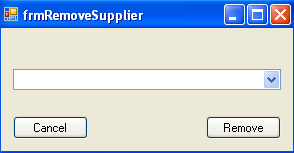
\includegraphics[scale=0.5]{frmRemoveSupplier_scrot}
	\makeatletter
\def\PY@reset{\let\PY@it=\relax \let\PY@bf=\relax%
    \let\PY@ul=\relax \let\PY@tc=\relax%
    \let\PY@bc=\relax \let\PY@ff=\relax}
\def\PY@tok#1{\csname PY@tok@#1\endcsname}
\def\PY@toks#1+{\ifx\relax#1\empty\else%
    \PY@tok{#1}\expandafter\PY@toks\fi}
\def\PY@do#1{\PY@bc{\PY@tc{\PY@ul{%
    \PY@it{\PY@bf{\PY@ff{#1}}}}}}}
\def\PY#1#2{\PY@reset\PY@toks#1+\relax+\PY@do{#2}}

\expandafter\def\csname PY@tok@gd\endcsname{\def\PY@tc##1{\textcolor[rgb]{0.63,0.00,0.00}{##1}}}
\expandafter\def\csname PY@tok@gu\endcsname{\let\PY@bf=\textbf\def\PY@tc##1{\textcolor[rgb]{0.50,0.00,0.50}{##1}}}
\expandafter\def\csname PY@tok@gt\endcsname{\def\PY@tc##1{\textcolor[rgb]{0.00,0.25,0.82}{##1}}}
\expandafter\def\csname PY@tok@gs\endcsname{\let\PY@bf=\textbf}
\expandafter\def\csname PY@tok@gr\endcsname{\def\PY@tc##1{\textcolor[rgb]{1.00,0.00,0.00}{##1}}}
\expandafter\def\csname PY@tok@cm\endcsname{\let\PY@it=\textit\def\PY@tc##1{\textcolor[rgb]{0.25,0.50,0.50}{##1}}}
\expandafter\def\csname PY@tok@vg\endcsname{\def\PY@tc##1{\textcolor[rgb]{0.10,0.09,0.49}{##1}}}
\expandafter\def\csname PY@tok@m\endcsname{\def\PY@tc##1{\textcolor[rgb]{0.40,0.40,0.40}{##1}}}
\expandafter\def\csname PY@tok@mh\endcsname{\def\PY@tc##1{\textcolor[rgb]{0.40,0.40,0.40}{##1}}}
\expandafter\def\csname PY@tok@go\endcsname{\def\PY@tc##1{\textcolor[rgb]{0.50,0.50,0.50}{##1}}}
\expandafter\def\csname PY@tok@ge\endcsname{\let\PY@it=\textit}
\expandafter\def\csname PY@tok@vc\endcsname{\def\PY@tc##1{\textcolor[rgb]{0.10,0.09,0.49}{##1}}}
\expandafter\def\csname PY@tok@il\endcsname{\def\PY@tc##1{\textcolor[rgb]{0.40,0.40,0.40}{##1}}}
\expandafter\def\csname PY@tok@cs\endcsname{\let\PY@it=\textit\def\PY@tc##1{\textcolor[rgb]{0.25,0.50,0.50}{##1}}}
\expandafter\def\csname PY@tok@cp\endcsname{\def\PY@tc##1{\textcolor[rgb]{0.74,0.48,0.00}{##1}}}
\expandafter\def\csname PY@tok@gi\endcsname{\def\PY@tc##1{\textcolor[rgb]{0.00,0.63,0.00}{##1}}}
\expandafter\def\csname PY@tok@gh\endcsname{\let\PY@bf=\textbf\def\PY@tc##1{\textcolor[rgb]{0.00,0.00,0.50}{##1}}}
\expandafter\def\csname PY@tok@ni\endcsname{\let\PY@bf=\textbf\def\PY@tc##1{\textcolor[rgb]{0.60,0.60,0.60}{##1}}}
\expandafter\def\csname PY@tok@nl\endcsname{\def\PY@tc##1{\textcolor[rgb]{0.63,0.63,0.00}{##1}}}
\expandafter\def\csname PY@tok@nn\endcsname{\let\PY@bf=\textbf\def\PY@tc##1{\textcolor[rgb]{0.00,0.00,1.00}{##1}}}
\expandafter\def\csname PY@tok@no\endcsname{\def\PY@tc##1{\textcolor[rgb]{0.53,0.00,0.00}{##1}}}
\expandafter\def\csname PY@tok@na\endcsname{\def\PY@tc##1{\textcolor[rgb]{0.49,0.56,0.16}{##1}}}
\expandafter\def\csname PY@tok@nb\endcsname{\def\PY@tc##1{\textcolor[rgb]{0.00,0.50,0.00}{##1}}}
\expandafter\def\csname PY@tok@nc\endcsname{\let\PY@bf=\textbf\def\PY@tc##1{\textcolor[rgb]{0.00,0.00,1.00}{##1}}}
\expandafter\def\csname PY@tok@nd\endcsname{\def\PY@tc##1{\textcolor[rgb]{0.67,0.13,1.00}{##1}}}
\expandafter\def\csname PY@tok@ne\endcsname{\let\PY@bf=\textbf\def\PY@tc##1{\textcolor[rgb]{0.82,0.25,0.23}{##1}}}
\expandafter\def\csname PY@tok@nf\endcsname{\def\PY@tc##1{\textcolor[rgb]{0.00,0.00,1.00}{##1}}}
\expandafter\def\csname PY@tok@si\endcsname{\let\PY@bf=\textbf\def\PY@tc##1{\textcolor[rgb]{0.73,0.40,0.53}{##1}}}
\expandafter\def\csname PY@tok@s2\endcsname{\def\PY@tc##1{\textcolor[rgb]{0.73,0.13,0.13}{##1}}}
\expandafter\def\csname PY@tok@vi\endcsname{\def\PY@tc##1{\textcolor[rgb]{0.10,0.09,0.49}{##1}}}
\expandafter\def\csname PY@tok@nt\endcsname{\let\PY@bf=\textbf\def\PY@tc##1{\textcolor[rgb]{0.00,0.50,0.00}{##1}}}
\expandafter\def\csname PY@tok@nv\endcsname{\def\PY@tc##1{\textcolor[rgb]{0.10,0.09,0.49}{##1}}}
\expandafter\def\csname PY@tok@s1\endcsname{\def\PY@tc##1{\textcolor[rgb]{0.73,0.13,0.13}{##1}}}
\expandafter\def\csname PY@tok@sh\endcsname{\def\PY@tc##1{\textcolor[rgb]{0.73,0.13,0.13}{##1}}}
\expandafter\def\csname PY@tok@sc\endcsname{\def\PY@tc##1{\textcolor[rgb]{0.73,0.13,0.13}{##1}}}
\expandafter\def\csname PY@tok@sx\endcsname{\def\PY@tc##1{\textcolor[rgb]{0.00,0.50,0.00}{##1}}}
\expandafter\def\csname PY@tok@bp\endcsname{\def\PY@tc##1{\textcolor[rgb]{0.00,0.50,0.00}{##1}}}
\expandafter\def\csname PY@tok@c1\endcsname{\let\PY@it=\textit\def\PY@tc##1{\textcolor[rgb]{0.25,0.50,0.50}{##1}}}
\expandafter\def\csname PY@tok@kc\endcsname{\let\PY@bf=\textbf\def\PY@tc##1{\textcolor[rgb]{0.00,0.50,0.00}{##1}}}
\expandafter\def\csname PY@tok@c\endcsname{\let\PY@it=\textit\def\PY@tc##1{\textcolor[rgb]{0.25,0.50,0.50}{##1}}}
\expandafter\def\csname PY@tok@mf\endcsname{\def\PY@tc##1{\textcolor[rgb]{0.40,0.40,0.40}{##1}}}
\expandafter\def\csname PY@tok@err\endcsname{\def\PY@bc##1{\setlength{\fboxsep}{0pt}\fcolorbox[rgb]{1.00,0.00,0.00}{1,1,1}{\strut ##1}}}
\expandafter\def\csname PY@tok@kd\endcsname{\let\PY@bf=\textbf\def\PY@tc##1{\textcolor[rgb]{0.00,0.50,0.00}{##1}}}
\expandafter\def\csname PY@tok@ss\endcsname{\def\PY@tc##1{\textcolor[rgb]{0.10,0.09,0.49}{##1}}}
\expandafter\def\csname PY@tok@sr\endcsname{\def\PY@tc##1{\textcolor[rgb]{0.73,0.40,0.53}{##1}}}
\expandafter\def\csname PY@tok@mo\endcsname{\def\PY@tc##1{\textcolor[rgb]{0.40,0.40,0.40}{##1}}}
\expandafter\def\csname PY@tok@kn\endcsname{\let\PY@bf=\textbf\def\PY@tc##1{\textcolor[rgb]{0.00,0.50,0.00}{##1}}}
\expandafter\def\csname PY@tok@mi\endcsname{\def\PY@tc##1{\textcolor[rgb]{0.40,0.40,0.40}{##1}}}
\expandafter\def\csname PY@tok@gp\endcsname{\let\PY@bf=\textbf\def\PY@tc##1{\textcolor[rgb]{0.00,0.00,0.50}{##1}}}
\expandafter\def\csname PY@tok@o\endcsname{\def\PY@tc##1{\textcolor[rgb]{0.40,0.40,0.40}{##1}}}
\expandafter\def\csname PY@tok@kr\endcsname{\let\PY@bf=\textbf\def\PY@tc##1{\textcolor[rgb]{0.00,0.50,0.00}{##1}}}
\expandafter\def\csname PY@tok@s\endcsname{\def\PY@tc##1{\textcolor[rgb]{0.73,0.13,0.13}{##1}}}
\expandafter\def\csname PY@tok@kp\endcsname{\def\PY@tc##1{\textcolor[rgb]{0.00,0.50,0.00}{##1}}}
\expandafter\def\csname PY@tok@w\endcsname{\def\PY@tc##1{\textcolor[rgb]{0.73,0.73,0.73}{##1}}}
\expandafter\def\csname PY@tok@kt\endcsname{\def\PY@tc##1{\textcolor[rgb]{0.69,0.00,0.25}{##1}}}
\expandafter\def\csname PY@tok@ow\endcsname{\let\PY@bf=\textbf\def\PY@tc##1{\textcolor[rgb]{0.67,0.13,1.00}{##1}}}
\expandafter\def\csname PY@tok@sb\endcsname{\def\PY@tc##1{\textcolor[rgb]{0.73,0.13,0.13}{##1}}}
\expandafter\def\csname PY@tok@k\endcsname{\let\PY@bf=\textbf\def\PY@tc##1{\textcolor[rgb]{0.00,0.50,0.00}{##1}}}
\expandafter\def\csname PY@tok@se\endcsname{\let\PY@bf=\textbf\def\PY@tc##1{\textcolor[rgb]{0.73,0.40,0.13}{##1}}}
\expandafter\def\csname PY@tok@sd\endcsname{\let\PY@it=\textit\def\PY@tc##1{\textcolor[rgb]{0.73,0.13,0.13}{##1}}}

\def\PYZbs{\char`\\}
\def\PYZus{\char`\_}
\def\PYZob{\char`\{}
\def\PYZcb{\char`\}}
\def\PYZca{\char`\^}
\def\PYZam{\char`\&}
\def\PYZlt{\char`\<}
\def\PYZgt{\char`\>}
\def\PYZsh{\char`\#}
\def\PYZpc{\char`\%}
\def\PYZdl{\char`\$}
\def\PYZti{\char`\~}
% for compatibility with earlier versions
\def\PYZat{@}
\def\PYZlb{[}
\def\PYZrb{]}
\makeatother

\begin{Verbatim}[commandchars=\\\{\}]
\PY{err}{�}\PY{err}{�}\PY{err}{�}\PY{k}{Imports} \PY{n+nn}{System.Data}
\PY{k}{Imports} \PY{n+nn}{System.Data.OleDb}

\PY{k}{Public} \PY{k}{Class} \PY{n+nc}{frmRemoveSupplier}
    \PY{c}{'THIS CODE SATISFIES SPECIFIC OBJECTIVE 7.}
    \PY{k}{Public} \PY{n}{accConnection} \PY{o+ow}{As} \PY{k}{New} \PY{n}{OleDbConnection}

    \PY{k}{Private} \PY{k}{Sub} \PY{n+nf}{frmRemoveSupplier\PYZus{}Load}\PY{p}{(}\PY{k}{ByVal} \PY{n}{sender} \PY{o+ow}{As} \PY{n}{System}\PY{p}{.}\PY{n}{Object}\PY{p}{,} \PY{n}{\PYZus{}}
                                       \PY{k}{ByVal} \PY{n}{e} \PY{o+ow}{As} \PY{n}{System}\PY{p}{.}\PY{n}{EventArgs}\PY{p}{)} \PY{k}{Handles} \PY{k}{MyBase}\PY{p}{.}\PY{n}{Load}

        \PY{c}{'Check if db connection is breathing.}
        \PY{c}{'If it isn't, resuscitate it.}
        \PY{k}{If} \PY{n}{frmLoginForm}\PY{p}{.}\PY{n}{accConnection}\PY{p}{.}\PY{n}{State} \PY{o}{\PYZlt{}\PYZgt{}} \PY{n}{ConnectionState}\PY{p}{.}\PY{n}{Open} \PY{k}{Then}
            \PY{n}{frmLoginForm}\PY{p}{.}\PY{n}{accConnection}\PY{p}{.}\PY{n}{Open}\PY{p}{(}\PY{p}{)}
        \PY{k}{End} \PY{k}{If}

        \PY{n}{accConnection} \PY{o}{=} \PY{n}{frmLoginForm}\PY{p}{.}\PY{n}{accConnection}
        \PY{k}{Dim} \PY{n}{strSQL} \PY{o+ow}{As} \PY{k+kt}{String} \PY{o}{=} \PY{l+s}{"}\PY{l+s}{SELECT supp\PYZus{}id,supp\PYZus{}name FROM Supplier}\PY{l+s}{"}
        \PY{k}{Dim} \PY{n}{da} \PY{o+ow}{As} \PY{k}{New} \PY{n}{OleDbDataAdapter}\PY{p}{(}\PY{n}{strSQL}\PY{p}{,} \PY{n}{accConnection}\PY{p}{)}
        \PY{k}{Dim} \PY{n}{ds} \PY{o+ow}{As} \PY{k}{New} \PY{n}{DataSet}

        \PY{n}{da}\PY{p}{.}\PY{n}{Fill}\PY{p}{(}\PY{n}{ds}\PY{p}{,} \PY{l+s}{"}\PY{l+s}{Supplier}\PY{l+s}{"}\PY{p}{)}

        \PY{k}{Dim} \PY{n}{dt} \PY{o+ow}{As} \PY{n}{DataTable} \PY{o}{=} \PY{n}{ds}\PY{p}{.}\PY{n}{Tables}\PY{p}{(}\PY{l+m+mi}{0}\PY{p}{)}
        \PY{k}{Dim} \PY{n}{dr} \PY{o+ow}{As} \PY{n}{DataRow}

        \PY{k}{For} \PY{k}{Each} \PY{n}{dr} \PY{o+ow}{In} \PY{n}{dt}\PY{p}{.}\PY{n}{Rows}\PY{p}{(}\PY{p}{)}
            \PY{c}{'Populate the box with the supplier names.}
            \PY{n}{txtcbSupplierRemove}\PY{p}{.}\PY{n}{Items}\PY{p}{.}\PY{n}{Add}\PY{p}{(}\PY{n}{dr}\PY{p}{(}\PY{l+s}{"}\PY{l+s}{supp\PYZus{}name}\PY{l+s}{"}\PY{p}{)}\PY{p}{)}
        \PY{k}{Next}

        \PY{n}{txtcbSupplierRemove}\PY{p}{.}\PY{n}{SelectedIndex} \PY{o}{=} \PY{o}{-}\PY{l+m+mi}{1}

    \PY{k}{End} \PY{k}{Sub}

    \PY{k}{Private} \PY{k}{Sub} \PY{n+nf}{btnRemove\PYZus{}Click}\PY{p}{(}\PY{k}{ByVal} \PY{n}{sender} \PY{o+ow}{As} \PY{n}{System}\PY{p}{.}\PY{n}{Object}\PY{p}{,} \PY{n}{\PYZus{}}
                                \PY{k}{ByVal} \PY{n}{e} \PY{o+ow}{As} \PY{n}{System}\PY{p}{.}\PY{n}{EventArgs}\PY{p}{)} \PY{k}{Handles} \PY{n}{btnRemove}\PY{p}{.}\PY{n}{Click}

        \PY{k}{Dim} \PY{n}{RemoveSupplierDataAdapter} \PY{o+ow}{As} \PY{k}{New} \PY{n}{OleDbDataAdapter}
        \PY{k}{Dim} \PY{n}{accCommand} \PY{o+ow}{As} \PY{k}{New} \PY{n}{OleDbCommand}
        \PY{k}{Dim} \PY{n}{cmdString} \PY{o+ow}{As} \PY{k+kt}{String} \PY{o}{=} \PY{l+s}{"}\PY{l+s}{DELETE * FROM Supplier WHERE supp\PYZus{}name = }\PY{l+s}{"} \PY{o}{\PYZam{}} \PY{n}{\PYZus{}}
                                    \PY{k}{Me}\PY{p}{.}\PY{n}{txtcbSupplierRemove}\PY{p}{.}\PY{n}{SelectedItem} \PY{o}{\PYZam{}} \PY{l+s}{"}\PY{l+s}{"}

        \PY{n}{accCommand}\PY{p}{.}\PY{n}{Connection} \PY{o}{=} \PY{n}{frmLoginForm}\PY{p}{.}\PY{n}{accConnection}
        \PY{n}{accCommand}\PY{p}{.}\PY{n}{CommandType} \PY{o}{=} \PY{n}{CommandType}\PY{p}{.}\PY{n}{Text}
        \PY{n}{accCommand}\PY{p}{.}\PY{n}{CommandText} \PY{o}{=} \PY{n}{cmdString}

        \PY{k}{Call} \PY{n}{RemoveParameters}\PY{p}{(}\PY{n}{accCommand}\PY{p}{)}
        \PY{c}{'Execute the query to delete the record from the db.}
        \PY{k}{Dim} \PY{n}{intRemove} \PY{o+ow}{As} \PY{k+kt}{Integer}

        \PY{k}{Try}
            \PY{n}{intRemove} \PY{o}{=} \PY{n}{accCommand}\PY{p}{.}\PY{n}{ExecuteNonQuery}\PY{p}{(}\PY{p}{)}
        \PY{k}{Catch} \PY{n}{ex} \PY{o+ow}{As} \PY{n}{Exception}
            \PY{n}{intRemove} \PY{o}{=} \PY{l+m+mi}{0}
            \PY{n}{MsgBox}\PY{p}{(}\PY{l+s}{"}\PY{l+s}{Maybe you should try deleting the associated component first?}\PY{l+s}{"}\PY{p}{)}
        \PY{k}{End} \PY{k}{Try}

        \PY{k}{If} \PY{n}{intRemove} \PY{o}{=} \PY{l+m+mi}{0} \PY{k}{Then}
            \PY{n}{MsgBox}\PY{p}{(}\PY{l+s}{"}\PY{l+s}{Data deletion failed.}\PY{l+s}{"}\PY{p}{)}
            \PY{c}{'Else, assume it went through OK.}
        \PY{k}{Else}
            \PY{n}{btnRemove}\PY{p}{.}\PY{n}{Enabled} \PY{o}{=} \PY{k}{False}
        \PY{k}{End} \PY{k}{If}

    \PY{k}{End} \PY{k}{Sub}

    \PY{k}{Private} \PY{k}{Sub} \PY{n+nf}{RemoveParameters}\PY{p}{(}\PY{k}{ByRef} \PY{n}{acccmd} \PY{o+ow}{As} \PY{n}{OleDbCommand}\PY{p}{)}
        \PY{n}{acccmd}\PY{p}{.}\PY{n}{Parameters}\PY{p}{.}\PY{n}{Add}\PY{p}{(}\PY{l+s}{"}\PY{l+s}{@supp\PYZus{}name}\PY{l+s}{"}\PY{p}{,} \PY{n}{OleDbType}\PY{p}{.}\PY{n}{Char}\PY{p}{)}\PY{p}{.}\PY{n}{Value} \PY{o}{=} \PY{n}{\PYZus{}}
                                    \PY{n}{txtcbSupplierRemove}\PY{p}{.}\PY{n}{SelectedItem}
    \PY{k}{End} \PY{k}{Sub}

    \PY{k}{Private} \PY{k}{Sub} \PY{n+nf}{btnCancel\PYZus{}Click}\PY{p}{(}\PY{k}{ByVal} \PY{n}{sender} \PY{o+ow}{As} \PY{n}{System}\PY{p}{.}\PY{n}{Object}\PY{p}{,} \PY{n}{\PYZus{}}
                                \PY{k}{ByVal} \PY{n}{e} \PY{o+ow}{As} \PY{n}{System}\PY{p}{.}\PY{n}{EventArgs}\PY{p}{)} \PY{k}{Handles} \PY{n}{btnCancel}\PY{p}{.}\PY{n}{Click}
        \PY{k}{Me}\PY{p}{.}\PY{n}{Close}\PY{p}{(}\PY{p}{)}
        \PY{n}{frmRemove}\PY{p}{.}\PY{n}{Show}\PY{p}{(}\PY{p}{)}
    \PY{k}{End} \PY{k}{Sub}
\PY{k}{End} \PY{k}{Class}
\end{Verbatim}
	
\subsection{frmRemoveComponent}
	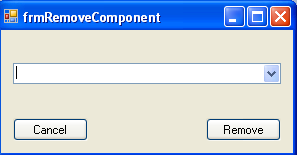
\includegraphics[scale=0.5]{frmRemoveComponent_scrot}
	\makeatletter
\def\PY@reset{\let\PY@it=\relax \let\PY@bf=\relax%
    \let\PY@ul=\relax \let\PY@tc=\relax%
    \let\PY@bc=\relax \let\PY@ff=\relax}
\def\PY@tok#1{\csname PY@tok@#1\endcsname}
\def\PY@toks#1+{\ifx\relax#1\empty\else%
    \PY@tok{#1}\expandafter\PY@toks\fi}
\def\PY@do#1{\PY@bc{\PY@tc{\PY@ul{%
    \PY@it{\PY@bf{\PY@ff{#1}}}}}}}
\def\PY#1#2{\PY@reset\PY@toks#1+\relax+\PY@do{#2}}

\expandafter\def\csname PY@tok@gd\endcsname{\def\PY@tc##1{\textcolor[rgb]{0.63,0.00,0.00}{##1}}}
\expandafter\def\csname PY@tok@gu\endcsname{\let\PY@bf=\textbf\def\PY@tc##1{\textcolor[rgb]{0.50,0.00,0.50}{##1}}}
\expandafter\def\csname PY@tok@gt\endcsname{\def\PY@tc##1{\textcolor[rgb]{0.00,0.25,0.82}{##1}}}
\expandafter\def\csname PY@tok@gs\endcsname{\let\PY@bf=\textbf}
\expandafter\def\csname PY@tok@gr\endcsname{\def\PY@tc##1{\textcolor[rgb]{1.00,0.00,0.00}{##1}}}
\expandafter\def\csname PY@tok@cm\endcsname{\let\PY@it=\textit\def\PY@tc##1{\textcolor[rgb]{0.25,0.50,0.50}{##1}}}
\expandafter\def\csname PY@tok@vg\endcsname{\def\PY@tc##1{\textcolor[rgb]{0.10,0.09,0.49}{##1}}}
\expandafter\def\csname PY@tok@m\endcsname{\def\PY@tc##1{\textcolor[rgb]{0.40,0.40,0.40}{##1}}}
\expandafter\def\csname PY@tok@mh\endcsname{\def\PY@tc##1{\textcolor[rgb]{0.40,0.40,0.40}{##1}}}
\expandafter\def\csname PY@tok@go\endcsname{\def\PY@tc##1{\textcolor[rgb]{0.50,0.50,0.50}{##1}}}
\expandafter\def\csname PY@tok@ge\endcsname{\let\PY@it=\textit}
\expandafter\def\csname PY@tok@vc\endcsname{\def\PY@tc##1{\textcolor[rgb]{0.10,0.09,0.49}{##1}}}
\expandafter\def\csname PY@tok@il\endcsname{\def\PY@tc##1{\textcolor[rgb]{0.40,0.40,0.40}{##1}}}
\expandafter\def\csname PY@tok@cs\endcsname{\let\PY@it=\textit\def\PY@tc##1{\textcolor[rgb]{0.25,0.50,0.50}{##1}}}
\expandafter\def\csname PY@tok@cp\endcsname{\def\PY@tc##1{\textcolor[rgb]{0.74,0.48,0.00}{##1}}}
\expandafter\def\csname PY@tok@gi\endcsname{\def\PY@tc##1{\textcolor[rgb]{0.00,0.63,0.00}{##1}}}
\expandafter\def\csname PY@tok@gh\endcsname{\let\PY@bf=\textbf\def\PY@tc##1{\textcolor[rgb]{0.00,0.00,0.50}{##1}}}
\expandafter\def\csname PY@tok@ni\endcsname{\let\PY@bf=\textbf\def\PY@tc##1{\textcolor[rgb]{0.60,0.60,0.60}{##1}}}
\expandafter\def\csname PY@tok@nl\endcsname{\def\PY@tc##1{\textcolor[rgb]{0.63,0.63,0.00}{##1}}}
\expandafter\def\csname PY@tok@nn\endcsname{\let\PY@bf=\textbf\def\PY@tc##1{\textcolor[rgb]{0.00,0.00,1.00}{##1}}}
\expandafter\def\csname PY@tok@no\endcsname{\def\PY@tc##1{\textcolor[rgb]{0.53,0.00,0.00}{##1}}}
\expandafter\def\csname PY@tok@na\endcsname{\def\PY@tc##1{\textcolor[rgb]{0.49,0.56,0.16}{##1}}}
\expandafter\def\csname PY@tok@nb\endcsname{\def\PY@tc##1{\textcolor[rgb]{0.00,0.50,0.00}{##1}}}
\expandafter\def\csname PY@tok@nc\endcsname{\let\PY@bf=\textbf\def\PY@tc##1{\textcolor[rgb]{0.00,0.00,1.00}{##1}}}
\expandafter\def\csname PY@tok@nd\endcsname{\def\PY@tc##1{\textcolor[rgb]{0.67,0.13,1.00}{##1}}}
\expandafter\def\csname PY@tok@ne\endcsname{\let\PY@bf=\textbf\def\PY@tc##1{\textcolor[rgb]{0.82,0.25,0.23}{##1}}}
\expandafter\def\csname PY@tok@nf\endcsname{\def\PY@tc##1{\textcolor[rgb]{0.00,0.00,1.00}{##1}}}
\expandafter\def\csname PY@tok@si\endcsname{\let\PY@bf=\textbf\def\PY@tc##1{\textcolor[rgb]{0.73,0.40,0.53}{##1}}}
\expandafter\def\csname PY@tok@s2\endcsname{\def\PY@tc##1{\textcolor[rgb]{0.73,0.13,0.13}{##1}}}
\expandafter\def\csname PY@tok@vi\endcsname{\def\PY@tc##1{\textcolor[rgb]{0.10,0.09,0.49}{##1}}}
\expandafter\def\csname PY@tok@nt\endcsname{\let\PY@bf=\textbf\def\PY@tc##1{\textcolor[rgb]{0.00,0.50,0.00}{##1}}}
\expandafter\def\csname PY@tok@nv\endcsname{\def\PY@tc##1{\textcolor[rgb]{0.10,0.09,0.49}{##1}}}
\expandafter\def\csname PY@tok@s1\endcsname{\def\PY@tc##1{\textcolor[rgb]{0.73,0.13,0.13}{##1}}}
\expandafter\def\csname PY@tok@sh\endcsname{\def\PY@tc##1{\textcolor[rgb]{0.73,0.13,0.13}{##1}}}
\expandafter\def\csname PY@tok@sc\endcsname{\def\PY@tc##1{\textcolor[rgb]{0.73,0.13,0.13}{##1}}}
\expandafter\def\csname PY@tok@sx\endcsname{\def\PY@tc##1{\textcolor[rgb]{0.00,0.50,0.00}{##1}}}
\expandafter\def\csname PY@tok@bp\endcsname{\def\PY@tc##1{\textcolor[rgb]{0.00,0.50,0.00}{##1}}}
\expandafter\def\csname PY@tok@c1\endcsname{\let\PY@it=\textit\def\PY@tc##1{\textcolor[rgb]{0.25,0.50,0.50}{##1}}}
\expandafter\def\csname PY@tok@kc\endcsname{\let\PY@bf=\textbf\def\PY@tc##1{\textcolor[rgb]{0.00,0.50,0.00}{##1}}}
\expandafter\def\csname PY@tok@c\endcsname{\let\PY@it=\textit\def\PY@tc##1{\textcolor[rgb]{0.25,0.50,0.50}{##1}}}
\expandafter\def\csname PY@tok@mf\endcsname{\def\PY@tc##1{\textcolor[rgb]{0.40,0.40,0.40}{##1}}}
\expandafter\def\csname PY@tok@err\endcsname{\def\PY@bc##1{\setlength{\fboxsep}{0pt}\fcolorbox[rgb]{1.00,0.00,0.00}{1,1,1}{\strut ##1}}}
\expandafter\def\csname PY@tok@kd\endcsname{\let\PY@bf=\textbf\def\PY@tc##1{\textcolor[rgb]{0.00,0.50,0.00}{##1}}}
\expandafter\def\csname PY@tok@ss\endcsname{\def\PY@tc##1{\textcolor[rgb]{0.10,0.09,0.49}{##1}}}
\expandafter\def\csname PY@tok@sr\endcsname{\def\PY@tc##1{\textcolor[rgb]{0.73,0.40,0.53}{##1}}}
\expandafter\def\csname PY@tok@mo\endcsname{\def\PY@tc##1{\textcolor[rgb]{0.40,0.40,0.40}{##1}}}
\expandafter\def\csname PY@tok@kn\endcsname{\let\PY@bf=\textbf\def\PY@tc##1{\textcolor[rgb]{0.00,0.50,0.00}{##1}}}
\expandafter\def\csname PY@tok@mi\endcsname{\def\PY@tc##1{\textcolor[rgb]{0.40,0.40,0.40}{##1}}}
\expandafter\def\csname PY@tok@gp\endcsname{\let\PY@bf=\textbf\def\PY@tc##1{\textcolor[rgb]{0.00,0.00,0.50}{##1}}}
\expandafter\def\csname PY@tok@o\endcsname{\def\PY@tc##1{\textcolor[rgb]{0.40,0.40,0.40}{##1}}}
\expandafter\def\csname PY@tok@kr\endcsname{\let\PY@bf=\textbf\def\PY@tc##1{\textcolor[rgb]{0.00,0.50,0.00}{##1}}}
\expandafter\def\csname PY@tok@s\endcsname{\def\PY@tc##1{\textcolor[rgb]{0.73,0.13,0.13}{##1}}}
\expandafter\def\csname PY@tok@kp\endcsname{\def\PY@tc##1{\textcolor[rgb]{0.00,0.50,0.00}{##1}}}
\expandafter\def\csname PY@tok@w\endcsname{\def\PY@tc##1{\textcolor[rgb]{0.73,0.73,0.73}{##1}}}
\expandafter\def\csname PY@tok@kt\endcsname{\def\PY@tc##1{\textcolor[rgb]{0.69,0.00,0.25}{##1}}}
\expandafter\def\csname PY@tok@ow\endcsname{\let\PY@bf=\textbf\def\PY@tc##1{\textcolor[rgb]{0.67,0.13,1.00}{##1}}}
\expandafter\def\csname PY@tok@sb\endcsname{\def\PY@tc##1{\textcolor[rgb]{0.73,0.13,0.13}{##1}}}
\expandafter\def\csname PY@tok@k\endcsname{\let\PY@bf=\textbf\def\PY@tc##1{\textcolor[rgb]{0.00,0.50,0.00}{##1}}}
\expandafter\def\csname PY@tok@se\endcsname{\let\PY@bf=\textbf\def\PY@tc##1{\textcolor[rgb]{0.73,0.40,0.13}{##1}}}
\expandafter\def\csname PY@tok@sd\endcsname{\let\PY@it=\textit\def\PY@tc##1{\textcolor[rgb]{0.73,0.13,0.13}{##1}}}

\def\PYZbs{\char`\\}
\def\PYZus{\char`\_}
\def\PYZob{\char`\{}
\def\PYZcb{\char`\}}
\def\PYZca{\char`\^}
\def\PYZam{\char`\&}
\def\PYZlt{\char`\<}
\def\PYZgt{\char`\>}
\def\PYZsh{\char`\#}
\def\PYZpc{\char`\%}
\def\PYZdl{\char`\$}
\def\PYZti{\char`\~}
% for compatibility with earlier versions
\def\PYZat{@}
\def\PYZlb{[}
\def\PYZrb{]}
\makeatother

\begin{Verbatim}[commandchars=\\\{\}]
\PY{err}{�}\PY{err}{�}\PY{err}{�}\PY{k}{Imports} \PY{n+nn}{System.Data}
\PY{k}{Imports} \PY{n+nn}{System.Data.OleDb}

\PY{k}{Class} \PY{n+nc}{frmRemoveComponent}
    \PY{c}{'THIS CODE SATISFIES SPECIFIC OBJECTIVE 8.}
    \PY{k}{Public} \PY{n}{accConnection} \PY{o+ow}{As} \PY{k}{New} \PY{n}{OleDbConnection}

    \PY{k}{Private} \PY{k}{Sub} \PY{n+nf}{frmRemoveComponent\PYZus{}Load}\PY{p}{(}\PY{k}{ByVal} \PY{n}{sender} \PY{o+ow}{As} \PY{n}{System}\PY{p}{.}\PY{n}{Object}\PY{p}{,} \PY{n}{\PYZus{}}
                                        \PY{k}{ByVal} \PY{n}{e} \PY{o+ow}{As} \PY{n}{System}\PY{p}{.}\PY{n}{EventArgs}\PY{p}{)} \PY{k}{Handles} \PY{k}{MyBase}\PY{p}{.}\PY{n}{Load}
        \PY{c}{'Check if the database connection is breathing.}
        \PY{c}{'If it isn't, resuscitate it.  :-)}
        \PY{k}{If} \PY{n}{frmLoginForm}\PY{p}{.}\PY{n}{accConnection}\PY{p}{.}\PY{n}{State} \PY{o}{\PYZlt{}\PYZgt{}} \PY{n}{ConnectionState}\PY{p}{.}\PY{n}{Open} \PY{k}{Then}
            \PY{n}{frmLoginForm}\PY{p}{.}\PY{n}{accConnection}\PY{p}{.}\PY{n}{Open}\PY{p}{(}\PY{p}{)}
        \PY{k}{End} \PY{k}{If}

        \PY{n}{accConnection} \PY{o}{=} \PY{n}{frmLoginForm}\PY{p}{.}\PY{n}{accConnection}
        \PY{k}{Dim} \PY{n}{strSQL} \PY{o+ow}{As} \PY{k+kt}{String} \PY{o}{=} \PY{l+s}{"}\PY{l+s}{SELECT comp\PYZus{}name FROM Component}\PY{l+s}{"}
        \PY{k}{Dim} \PY{n}{da} \PY{o+ow}{As} \PY{k}{New} \PY{n}{OleDbDataAdapter}\PY{p}{(}\PY{n}{strSQL}\PY{p}{,} \PY{n}{accConnection}\PY{p}{)}
        \PY{k}{Dim} \PY{n}{ds} \PY{o+ow}{As} \PY{k}{New} \PY{n}{DataSet}

        \PY{n}{da}\PY{p}{.}\PY{n}{Fill}\PY{p}{(}\PY{n}{ds}\PY{p}{,} \PY{l+s}{"}\PY{l+s}{Component}\PY{l+s}{"}\PY{p}{)}

        \PY{k}{Dim} \PY{n}{dt} \PY{o+ow}{As} \PY{n}{DataTable} \PY{o}{=} \PY{n}{ds}\PY{p}{.}\PY{n}{Tables}\PY{p}{(}\PY{l+m+mi}{0}\PY{p}{)}
        \PY{k}{Dim} \PY{n}{dr} \PY{o+ow}{As} \PY{n}{DataRow}

        \PY{k}{For} \PY{k}{Each} \PY{n}{dr} \PY{o+ow}{In} \PY{n}{dt}\PY{p}{.}\PY{n}{Rows}\PY{p}{(}\PY{p}{)}
            \PY{c}{'List component names in the box.}
            \PY{n}{txtcbComponentRemove}\PY{p}{.}\PY{n}{Items}\PY{p}{.}\PY{n}{Add}\PY{p}{(}\PY{n}{dr}\PY{p}{(}\PY{l+s}{"}\PY{l+s}{comp\PYZus{}name}\PY{l+s}{"}\PY{p}{)}\PY{p}{)}
        \PY{k}{Next}

        \PY{n}{txtcbComponentRemove}\PY{p}{.}\PY{n}{SelectedIndex} \PY{o}{=} \PY{o}{-}\PY{l+m+mi}{1}

    \PY{k}{End} \PY{k}{Sub}

    \PY{k}{Private} \PY{k}{Sub} \PY{n+nf}{btnRemove\PYZus{}Click}\PY{p}{(}\PY{k}{ByVal} \PY{n}{sender} \PY{o+ow}{As} \PY{n}{System}\PY{p}{.}\PY{n}{Object}\PY{p}{,} \PY{n}{\PYZus{}}
                                \PY{k}{ByVal} \PY{n}{e} \PY{o+ow}{As} \PY{n}{System}\PY{p}{.}\PY{n}{EventArgs}\PY{p}{)} \PY{k}{Handles} \PY{n}{btnRemove}\PY{p}{.}\PY{n}{Click}

        \PY{k}{Dim} \PY{n}{cmdString} \PY{o+ow}{As} \PY{k+kt}{String} \PY{o}{=} \PY{l+s}{"}\PY{l+s}{DELETE * FROM Component WHERE comp\PYZus{}name = '}\PY{l+s}{"} \PY{o}{\PYZam{}} \PY{n}{\PYZus{}}
                                    \PY{k}{Me}\PY{p}{.}\PY{n}{txtcbComponentRemove}\PY{p}{.}\PY{n}{SelectedItem} \PY{o}{\PYZam{}} \PY{l+s}{"}\PY{l+s}{'}\PY{l+s}{"}
        \PY{k}{Dim} \PY{n}{da} \PY{o+ow}{As} \PY{k}{New} \PY{n}{OleDbDataAdapter}\PY{p}{(}\PY{n}{cmdString}\PY{p}{,} \PY{n}{accConnection}\PY{p}{)}
        \PY{k}{Dim} \PY{n}{ds} \PY{o+ow}{As} \PY{k}{New} \PY{n}{DataSet}
        \PY{k}{Dim} \PY{n}{accCommand} \PY{o+ow}{As} \PY{k}{New} \PY{n}{OleDbCommand}
        \PY{k}{Dim} \PY{n}{intRemove} \PY{o+ow}{As} \PY{k+kt}{Integer}

        \PY{n}{accCommand}\PY{p}{.}\PY{n}{Connection} \PY{o}{=} \PY{n}{frmLoginForm}\PY{p}{.}\PY{n}{accConnection}
        \PY{n}{accCommand}\PY{p}{.}\PY{n}{CommandType} \PY{o}{=} \PY{n}{CommandType}\PY{p}{.}\PY{n}{Text}
        \PY{n}{accCommand}\PY{p}{.}\PY{n}{CommandText} \PY{o}{=} \PY{n}{cmdString}

        \PY{n}{intRemove} \PY{o}{=} \PY{n}{accCommand}\PY{p}{.}\PY{n}{ExecuteNonQuery}\PY{p}{(}\PY{p}{)}

        \PY{k}{If} \PY{n}{intRemove} \PY{o}{=} \PY{l+m+mi}{0} \PY{k}{Then}
            \PY{n}{MsgBox}\PY{p}{(}\PY{l+s}{"}\PY{l+s}{Data deletion failed.}\PY{l+s}{"}\PY{p}{)}
            \PY{c}{'Else, assume it went through OK.}
        \PY{k}{Else}
            \PY{n}{btnRemove}\PY{p}{.}\PY{n}{Enabled} \PY{o}{=} \PY{k}{False}
        \PY{k}{End} \PY{k}{If}

    \PY{k}{End} \PY{k}{Sub}

    \PY{k}{Private} \PY{k}{Sub} \PY{n+nf}{RemoveParameters}\PY{p}{(}\PY{k}{ByRef} \PY{n}{acccmd} \PY{o+ow}{As} \PY{n}{OleDbCommand}\PY{p}{)}
        \PY{n}{acccmd}\PY{p}{.}\PY{n}{Parameters}\PY{p}{.}\PY{n}{Add}\PY{p}{(}\PY{l+s}{"}\PY{l+s}{@comp\PYZus{}name}\PY{l+s}{"}\PY{p}{,} \PY{n}{OleDbType}\PY{p}{.}\PY{n}{Char}\PY{p}{)}\PY{p}{.}\PY{n}{Value} \PY{o}{=} \PY{n}{\PYZus{}}
                                \PY{n}{txtcbComponentRemove}\PY{p}{.}\PY{n}{SelectedItem}
    \PY{k}{End} \PY{k}{Sub}

    \PY{k}{Private} \PY{k}{Sub} \PY{n+nf}{btnCancel\PYZus{}Click}\PY{p}{(}\PY{k}{ByVal} \PY{n}{sender} \PY{o+ow}{As} \PY{n}{System}\PY{p}{.}\PY{n}{Object}\PY{p}{,} \PY{n}{\PYZus{}}
                                \PY{k}{ByVal} \PY{n}{e} \PY{o+ow}{As} \PY{n}{System}\PY{p}{.}\PY{n}{EventArgs}\PY{p}{)} \PY{k}{Handles} \PY{n}{btnCancel}\PY{p}{.}\PY{n}{Click}
        \PY{k}{Me}\PY{p}{.}\PY{n}{Close}\PY{p}{(}\PY{p}{)}
        \PY{n}{frmRemove}\PY{p}{.}\PY{n}{Show}\PY{p}{(}\PY{p}{)}
    \PY{k}{End} \PY{k}{Sub}

\PY{k}{End} \PY{k}{Class}
\end{Verbatim}

\subsection{frmList}
	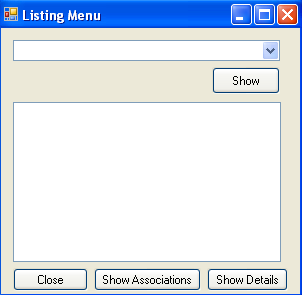
\includegraphics[scale=0.5]{frmList_scrot}
	\makeatletter
\def\PY@reset{\let\PY@it=\relax \let\PY@bf=\relax%
    \let\PY@ul=\relax \let\PY@tc=\relax%
    \let\PY@bc=\relax \let\PY@ff=\relax}
\def\PY@tok#1{\csname PY@tok@#1\endcsname}
\def\PY@toks#1+{\ifx\relax#1\empty\else%
    \PY@tok{#1}\expandafter\PY@toks\fi}
\def\PY@do#1{\PY@bc{\PY@tc{\PY@ul{%
    \PY@it{\PY@bf{\PY@ff{#1}}}}}}}
\def\PY#1#2{\PY@reset\PY@toks#1+\relax+\PY@do{#2}}

\expandafter\def\csname PY@tok@gd\endcsname{\def\PY@tc##1{\textcolor[rgb]{0.63,0.00,0.00}{##1}}}
\expandafter\def\csname PY@tok@gu\endcsname{\let\PY@bf=\textbf\def\PY@tc##1{\textcolor[rgb]{0.50,0.00,0.50}{##1}}}
\expandafter\def\csname PY@tok@gt\endcsname{\def\PY@tc##1{\textcolor[rgb]{0.00,0.25,0.82}{##1}}}
\expandafter\def\csname PY@tok@gs\endcsname{\let\PY@bf=\textbf}
\expandafter\def\csname PY@tok@gr\endcsname{\def\PY@tc##1{\textcolor[rgb]{1.00,0.00,0.00}{##1}}}
\expandafter\def\csname PY@tok@cm\endcsname{\let\PY@it=\textit\def\PY@tc##1{\textcolor[rgb]{0.25,0.50,0.50}{##1}}}
\expandafter\def\csname PY@tok@vg\endcsname{\def\PY@tc##1{\textcolor[rgb]{0.10,0.09,0.49}{##1}}}
\expandafter\def\csname PY@tok@m\endcsname{\def\PY@tc##1{\textcolor[rgb]{0.40,0.40,0.40}{##1}}}
\expandafter\def\csname PY@tok@mh\endcsname{\def\PY@tc##1{\textcolor[rgb]{0.40,0.40,0.40}{##1}}}
\expandafter\def\csname PY@tok@go\endcsname{\def\PY@tc##1{\textcolor[rgb]{0.50,0.50,0.50}{##1}}}
\expandafter\def\csname PY@tok@ge\endcsname{\let\PY@it=\textit}
\expandafter\def\csname PY@tok@vc\endcsname{\def\PY@tc##1{\textcolor[rgb]{0.10,0.09,0.49}{##1}}}
\expandafter\def\csname PY@tok@il\endcsname{\def\PY@tc##1{\textcolor[rgb]{0.40,0.40,0.40}{##1}}}
\expandafter\def\csname PY@tok@cs\endcsname{\let\PY@it=\textit\def\PY@tc##1{\textcolor[rgb]{0.25,0.50,0.50}{##1}}}
\expandafter\def\csname PY@tok@cp\endcsname{\def\PY@tc##1{\textcolor[rgb]{0.74,0.48,0.00}{##1}}}
\expandafter\def\csname PY@tok@gi\endcsname{\def\PY@tc##1{\textcolor[rgb]{0.00,0.63,0.00}{##1}}}
\expandafter\def\csname PY@tok@gh\endcsname{\let\PY@bf=\textbf\def\PY@tc##1{\textcolor[rgb]{0.00,0.00,0.50}{##1}}}
\expandafter\def\csname PY@tok@ni\endcsname{\let\PY@bf=\textbf\def\PY@tc##1{\textcolor[rgb]{0.60,0.60,0.60}{##1}}}
\expandafter\def\csname PY@tok@nl\endcsname{\def\PY@tc##1{\textcolor[rgb]{0.63,0.63,0.00}{##1}}}
\expandafter\def\csname PY@tok@nn\endcsname{\let\PY@bf=\textbf\def\PY@tc##1{\textcolor[rgb]{0.00,0.00,1.00}{##1}}}
\expandafter\def\csname PY@tok@no\endcsname{\def\PY@tc##1{\textcolor[rgb]{0.53,0.00,0.00}{##1}}}
\expandafter\def\csname PY@tok@na\endcsname{\def\PY@tc##1{\textcolor[rgb]{0.49,0.56,0.16}{##1}}}
\expandafter\def\csname PY@tok@nb\endcsname{\def\PY@tc##1{\textcolor[rgb]{0.00,0.50,0.00}{##1}}}
\expandafter\def\csname PY@tok@nc\endcsname{\let\PY@bf=\textbf\def\PY@tc##1{\textcolor[rgb]{0.00,0.00,1.00}{##1}}}
\expandafter\def\csname PY@tok@nd\endcsname{\def\PY@tc##1{\textcolor[rgb]{0.67,0.13,1.00}{##1}}}
\expandafter\def\csname PY@tok@ne\endcsname{\let\PY@bf=\textbf\def\PY@tc##1{\textcolor[rgb]{0.82,0.25,0.23}{##1}}}
\expandafter\def\csname PY@tok@nf\endcsname{\def\PY@tc##1{\textcolor[rgb]{0.00,0.00,1.00}{##1}}}
\expandafter\def\csname PY@tok@si\endcsname{\let\PY@bf=\textbf\def\PY@tc##1{\textcolor[rgb]{0.73,0.40,0.53}{##1}}}
\expandafter\def\csname PY@tok@s2\endcsname{\def\PY@tc##1{\textcolor[rgb]{0.73,0.13,0.13}{##1}}}
\expandafter\def\csname PY@tok@vi\endcsname{\def\PY@tc##1{\textcolor[rgb]{0.10,0.09,0.49}{##1}}}
\expandafter\def\csname PY@tok@nt\endcsname{\let\PY@bf=\textbf\def\PY@tc##1{\textcolor[rgb]{0.00,0.50,0.00}{##1}}}
\expandafter\def\csname PY@tok@nv\endcsname{\def\PY@tc##1{\textcolor[rgb]{0.10,0.09,0.49}{##1}}}
\expandafter\def\csname PY@tok@s1\endcsname{\def\PY@tc##1{\textcolor[rgb]{0.73,0.13,0.13}{##1}}}
\expandafter\def\csname PY@tok@sh\endcsname{\def\PY@tc##1{\textcolor[rgb]{0.73,0.13,0.13}{##1}}}
\expandafter\def\csname PY@tok@sc\endcsname{\def\PY@tc##1{\textcolor[rgb]{0.73,0.13,0.13}{##1}}}
\expandafter\def\csname PY@tok@sx\endcsname{\def\PY@tc##1{\textcolor[rgb]{0.00,0.50,0.00}{##1}}}
\expandafter\def\csname PY@tok@bp\endcsname{\def\PY@tc##1{\textcolor[rgb]{0.00,0.50,0.00}{##1}}}
\expandafter\def\csname PY@tok@c1\endcsname{\let\PY@it=\textit\def\PY@tc##1{\textcolor[rgb]{0.25,0.50,0.50}{##1}}}
\expandafter\def\csname PY@tok@kc\endcsname{\let\PY@bf=\textbf\def\PY@tc##1{\textcolor[rgb]{0.00,0.50,0.00}{##1}}}
\expandafter\def\csname PY@tok@c\endcsname{\let\PY@it=\textit\def\PY@tc##1{\textcolor[rgb]{0.25,0.50,0.50}{##1}}}
\expandafter\def\csname PY@tok@mf\endcsname{\def\PY@tc##1{\textcolor[rgb]{0.40,0.40,0.40}{##1}}}
\expandafter\def\csname PY@tok@err\endcsname{\def\PY@bc##1{\setlength{\fboxsep}{0pt}\fcolorbox[rgb]{1.00,0.00,0.00}{1,1,1}{\strut ##1}}}
\expandafter\def\csname PY@tok@kd\endcsname{\let\PY@bf=\textbf\def\PY@tc##1{\textcolor[rgb]{0.00,0.50,0.00}{##1}}}
\expandafter\def\csname PY@tok@ss\endcsname{\def\PY@tc##1{\textcolor[rgb]{0.10,0.09,0.49}{##1}}}
\expandafter\def\csname PY@tok@sr\endcsname{\def\PY@tc##1{\textcolor[rgb]{0.73,0.40,0.53}{##1}}}
\expandafter\def\csname PY@tok@mo\endcsname{\def\PY@tc##1{\textcolor[rgb]{0.40,0.40,0.40}{##1}}}
\expandafter\def\csname PY@tok@kn\endcsname{\let\PY@bf=\textbf\def\PY@tc##1{\textcolor[rgb]{0.00,0.50,0.00}{##1}}}
\expandafter\def\csname PY@tok@mi\endcsname{\def\PY@tc##1{\textcolor[rgb]{0.40,0.40,0.40}{##1}}}
\expandafter\def\csname PY@tok@gp\endcsname{\let\PY@bf=\textbf\def\PY@tc##1{\textcolor[rgb]{0.00,0.00,0.50}{##1}}}
\expandafter\def\csname PY@tok@o\endcsname{\def\PY@tc##1{\textcolor[rgb]{0.40,0.40,0.40}{##1}}}
\expandafter\def\csname PY@tok@kr\endcsname{\let\PY@bf=\textbf\def\PY@tc##1{\textcolor[rgb]{0.00,0.50,0.00}{##1}}}
\expandafter\def\csname PY@tok@s\endcsname{\def\PY@tc##1{\textcolor[rgb]{0.73,0.13,0.13}{##1}}}
\expandafter\def\csname PY@tok@kp\endcsname{\def\PY@tc##1{\textcolor[rgb]{0.00,0.50,0.00}{##1}}}
\expandafter\def\csname PY@tok@w\endcsname{\def\PY@tc##1{\textcolor[rgb]{0.73,0.73,0.73}{##1}}}
\expandafter\def\csname PY@tok@kt\endcsname{\def\PY@tc##1{\textcolor[rgb]{0.69,0.00,0.25}{##1}}}
\expandafter\def\csname PY@tok@ow\endcsname{\let\PY@bf=\textbf\def\PY@tc##1{\textcolor[rgb]{0.67,0.13,1.00}{##1}}}
\expandafter\def\csname PY@tok@sb\endcsname{\def\PY@tc##1{\textcolor[rgb]{0.73,0.13,0.13}{##1}}}
\expandafter\def\csname PY@tok@k\endcsname{\let\PY@bf=\textbf\def\PY@tc##1{\textcolor[rgb]{0.00,0.50,0.00}{##1}}}
\expandafter\def\csname PY@tok@se\endcsname{\let\PY@bf=\textbf\def\PY@tc##1{\textcolor[rgb]{0.73,0.40,0.13}{##1}}}
\expandafter\def\csname PY@tok@sd\endcsname{\let\PY@it=\textit\def\PY@tc##1{\textcolor[rgb]{0.73,0.13,0.13}{##1}}}

\def\PYZbs{\char`\\}
\def\PYZus{\char`\_}
\def\PYZob{\char`\{}
\def\PYZcb{\char`\}}
\def\PYZca{\char`\^}
\def\PYZam{\char`\&}
\def\PYZlt{\char`\<}
\def\PYZgt{\char`\>}
\def\PYZsh{\char`\#}
\def\PYZpc{\char`\%}
\def\PYZdl{\char`\$}
\def\PYZti{\char`\~}
% for compatibility with earlier versions
\def\PYZat{@}
\def\PYZlb{[}
\def\PYZrb{]}
\makeatother

\begin{Verbatim}[commandchars=\\\{\}]
\PY{err}{�}\PY{err}{�}\PY{err}{�}\PY{k}{Imports} \PY{n+nn}{System.Data}
\PY{k}{Imports} \PY{n+nn}{System.Data.OleDb}

\PY{k}{Public} \PY{k}{Class} \PY{n+nc}{frmList}
    \PY{c}{'THIS CODE SATISFIES SPECIFIC OBJECTIVES 9, 10, 11.}
    \PY{k}{Public} \PY{n}{accConnection} \PY{o+ow}{As} \PY{k}{New} \PY{n}{OleDbConnection}

    \PY{c}{'I think this is a better way of doing the listing [1] - fewer buttons}
    \PY{c}{'just a dropdown list which can be added to without having to create}
    \PY{c}{'another form}

    \PY{c}{'[1] - compared to the previous separate frmList[Customer|Supplier] etc.}

    \PY{k}{Private} \PY{k}{Sub} \PY{n+nf}{frmList\PYZus{}Load}\PY{p}{(}\PY{k}{ByVal} \PY{n}{sender} \PY{o+ow}{As} \PY{n}{System}\PY{p}{.}\PY{n}{Object}\PY{p}{,} \PY{n}{\PYZus{}}
                             \PY{k}{ByVal} \PY{n}{e} \PY{o+ow}{As} \PY{n}{System}\PY{p}{.}\PY{n}{EventArgs}\PY{p}{)} \PY{k}{Handles} \PY{k}{MyBase}\PY{p}{.}\PY{n}{Load}

        \PY{c}{'Check if db connection is breathing.}
        \PY{c}{'If it isn't, resuscitate it.  :)}
        \PY{k}{If} \PY{n}{frmLoginForm}\PY{p}{.}\PY{n}{accConnection}\PY{p}{.}\PY{n}{State} \PY{o}{\PYZlt{}\PYZgt{}} \PY{n}{ConnectionState}\PY{p}{.}\PY{n}{Open} \PY{k}{Then}
            \PY{n}{frmLoginForm}\PY{p}{.}\PY{n}{accConnection}\PY{p}{.}\PY{n}{Open}\PY{p}{(}\PY{p}{)}
        \PY{k}{End} \PY{k}{If}

        \PY{c}{'Populate the options list box with the following values.}
        \PY{n}{cbtxtListOptions}\PY{p}{.}\PY{n}{Items}\PY{p}{.}\PY{n}{Add}\PY{p}{(}\PY{l+s}{"}\PY{l+s}{Customers}\PY{l+s}{"}\PY{p}{)}
        \PY{n}{cbtxtListOptions}\PY{p}{.}\PY{n}{Items}\PY{p}{.}\PY{n}{Add}\PY{p}{(}\PY{l+s}{"}\PY{l+s}{Suppliers}\PY{l+s}{"}\PY{p}{)}
        \PY{n}{cbtxtListOptions}\PY{p}{.}\PY{n}{Items}\PY{p}{.}\PY{n}{Add}\PY{p}{(}\PY{l+s}{"}\PY{l+s}{Components}\PY{l+s}{"}\PY{p}{)}
    \PY{k}{End} \PY{k}{Sub}

    \PY{k}{Private} \PY{k}{Sub} \PY{n+nf}{cbtxtListOptions\PYZus{}SelectedIndexChanged}\PY{p}{(}\PY{k}{ByVal} \PY{n}{sender} \PY{o+ow}{As} \PY{n}{System}\PY{p}{.}\PY{n}{Object}\PY{p}{,} \PY{k}{ByVal} \PY{n}{e} \PY{o+ow}{As} \PY{n}{System}\PY{p}{.}\PY{n}{EventArgs}\PY{p}{)} \PY{k}{Handles} \PY{n}{cbtxtListOptions}\PY{p}{.}\PY{n}{SelectedIndexChanged}

        \PY{k}{Dim} \PY{n}{cmdString} \PY{o+ow}{As} \PY{k+kt}{String} \PY{o}{=} \PY{l+s}{"}\PY{l+s}{"} \PY{c}{'Initially blank.}
        \PY{n}{accConnection} \PY{o}{=} \PY{n}{frmLoginForm}\PY{p}{.}\PY{n}{accConnection}
        \PY{k}{Dim} \PY{n}{ds} \PY{o+ow}{As} \PY{k}{New} \PY{n}{DataSet}
        \PY{k}{Dim} \PY{n}{dr} \PY{o+ow}{As} \PY{n}{DataRow}

        \PY{c}{'da0, da1, da2}
        \PY{c}{'dt0, dt1, dt2}
        \PY{c}{'Declared within this if statement to make the program recognise }
        \PY{c}{'the change in cmdString and so know where to look.}
        \PY{c}{'Named da\PYZlt{}num\PYZgt{} and dt\PYZlt{}num\PYZgt{} to differentiate between different ifs.}

        \PY{c}{'Populate the list box with the result of the query - Customers.}
        \PY{k}{If} \PY{n}{cbtxtListOptions}\PY{p}{.}\PY{n}{Text} \PY{o}{=} \PY{l+s}{"}\PY{l+s}{Customers}\PY{l+s}{"} \PY{k}{Then}
            \PY{n}{cmdString} \PY{o}{=} \PY{l+s}{"}\PY{l+s}{SELECT cust\PYZus{}name FROM Customer}\PY{l+s}{"}
            \PY{c}{'Now clear the box if the selection changes.}
            \PY{n}{lbList}\PY{p}{.}\PY{n}{Items}\PY{p}{.}\PY{n}{Clear}\PY{p}{(}\PY{p}{)}
            \PY{k}{Dim} \PY{n}{da0} \PY{o+ow}{As} \PY{k}{New} \PY{n}{OleDbDataAdapter}\PY{p}{(}\PY{n}{cmdString}\PY{p}{,} \PY{n}{accConnection}\PY{p}{)}
            \PY{n}{da0}\PY{p}{.}\PY{n}{Fill}\PY{p}{(}\PY{n}{ds}\PY{p}{,} \PY{l+s}{"}\PY{l+s}{Customer}\PY{l+s}{"}\PY{p}{)}
            \PY{k}{Dim} \PY{n}{dt0} \PY{o+ow}{As} \PY{n}{DataTable} \PY{o}{=} \PY{n}{ds}\PY{p}{.}\PY{n}{Tables}\PY{p}{(}\PY{l+m+mi}{0}\PY{p}{)}
            \PY{k}{For} \PY{k}{Each} \PY{n}{dr} \PY{o+ow}{In} \PY{n}{dt0}\PY{p}{.}\PY{n}{Rows}\PY{p}{(}\PY{p}{)}
                \PY{n}{lbList}\PY{p}{.}\PY{n}{Items}\PY{p}{.}\PY{n}{Add}\PY{p}{(}\PY{n}{dr}\PY{p}{(}\PY{l+s}{"}\PY{l+s}{cust\PYZus{}name}\PY{l+s}{"}\PY{p}{)}\PY{p}{)}
            \PY{k}{Next}
            \PY{c}{'Populate the list box with the result of the query - Suppliers.}
        \PY{k}{ElseIf} \PY{n}{cbtxtListOptions}\PY{p}{.}\PY{n}{Text} \PY{o}{=} \PY{l+s}{"}\PY{l+s}{Suppliers}\PY{l+s}{"} \PY{k}{Then}
            \PY{n}{cmdString} \PY{o}{=} \PY{l+s}{"}\PY{l+s}{SELECT supp\PYZus{}name FROM Supplier}\PY{l+s}{"}
            \PY{c}{'Now clear the box if the selection changes.}
            \PY{n}{lbList}\PY{p}{.}\PY{n}{Items}\PY{p}{.}\PY{n}{Clear}\PY{p}{(}\PY{p}{)}
            \PY{k}{Dim} \PY{n}{da1} \PY{o+ow}{As} \PY{k}{New} \PY{n}{OleDbDataAdapter}\PY{p}{(}\PY{n}{cmdString}\PY{p}{,} \PY{n}{accConnection}\PY{p}{)}
            \PY{n}{da1}\PY{p}{.}\PY{n}{Fill}\PY{p}{(}\PY{n}{ds}\PY{p}{,} \PY{l+s}{"}\PY{l+s}{Supplier}\PY{l+s}{"}\PY{p}{)}
            \PY{k}{Dim} \PY{n}{dt1} \PY{o+ow}{As} \PY{n}{DataTable} \PY{o}{=} \PY{n}{ds}\PY{p}{.}\PY{n}{Tables}\PY{p}{(}\PY{l+m+mi}{0}\PY{p}{)}
            \PY{k}{For} \PY{k}{Each} \PY{n}{dr} \PY{o+ow}{In} \PY{n}{dt1}\PY{p}{.}\PY{n}{Rows}\PY{p}{(}\PY{p}{)}
                \PY{n}{lbList}\PY{p}{.}\PY{n}{Items}\PY{p}{.}\PY{n}{Add}\PY{p}{(}\PY{n}{dr}\PY{p}{(}\PY{l+s}{"}\PY{l+s}{supp\PYZus{}name}\PY{l+s}{"}\PY{p}{)}\PY{p}{)}
            \PY{k}{Next}
            \PY{c}{'Populate the list box with the result of the query - Components.}
        \PY{k}{ElseIf} \PY{n}{cbtxtListOptions}\PY{p}{.}\PY{n}{Text} \PY{o}{=} \PY{l+s}{"}\PY{l+s}{Components}\PY{l+s}{"} \PY{k}{Then}
            \PY{n}{cmdString} \PY{o}{=} \PY{l+s}{"}\PY{l+s}{SELECT comp\PYZus{}name FROM Component}\PY{l+s}{"}
            \PY{c}{'Now clear the box if the selection changes.}
            \PY{n}{lbList}\PY{p}{.}\PY{n}{Items}\PY{p}{.}\PY{n}{Clear}\PY{p}{(}\PY{p}{)}
            \PY{k}{Dim} \PY{n}{da2} \PY{o+ow}{As} \PY{k}{New} \PY{n}{OleDbDataAdapter}\PY{p}{(}\PY{n}{cmdString}\PY{p}{,} \PY{n}{accConnection}\PY{p}{)}
            \PY{n}{da2}\PY{p}{.}\PY{n}{Fill}\PY{p}{(}\PY{n}{ds}\PY{p}{,} \PY{l+s}{"}\PY{l+s}{Component}\PY{l+s}{"}\PY{p}{)}
            \PY{k}{Dim} \PY{n}{dt2} \PY{o+ow}{As} \PY{n}{DataTable} \PY{o}{=} \PY{n}{ds}\PY{p}{.}\PY{n}{Tables}\PY{p}{(}\PY{l+m+mi}{0}\PY{p}{)}
            \PY{k}{For} \PY{k}{Each} \PY{n}{dr} \PY{o+ow}{In} \PY{n}{dt2}\PY{p}{.}\PY{n}{Rows}\PY{p}{(}\PY{p}{)}
                \PY{n}{lbList}\PY{p}{.}\PY{n}{Items}\PY{p}{.}\PY{n}{Add}\PY{p}{(}\PY{n}{dr}\PY{p}{(}\PY{l+s}{"}\PY{l+s}{comp\PYZus{}name}\PY{l+s}{"}\PY{p}{)}\PY{p}{)}
            \PY{k}{Next}
        \PY{k}{End} \PY{k}{If}
    \PY{k}{End} \PY{k}{Sub}

    \PY{k}{Private} \PY{k}{Sub} \PY{n+nf}{btnSearch\PYZus{}Click}\PY{p}{(}\PY{k}{ByVal} \PY{n}{sender} \PY{o+ow}{As} \PY{n}{System}\PY{p}{.}\PY{n}{Object}\PY{p}{,} \PY{k}{ByVal} \PY{n}{e} \PY{o+ow}{As} \PY{n}{System}\PY{p}{.}\PY{n}{EventArgs}\PY{p}{)} \PY{k}{Handles} \PY{n}{btnSearch}\PY{p}{.}\PY{n}{Click}
        \PY{c}{'Implement searching of customers, suppliers, and components.  OBJECTIVE 17.}

        \PY{n}{accConnection} \PY{o}{=} \PY{n}{frmLoginForm}\PY{p}{.}\PY{n}{accConnection}
        \PY{k}{Dim} \PY{n}{ds} \PY{o+ow}{As} \PY{k}{New} \PY{n}{DataSet}
        \PY{k}{Dim} \PY{n}{dr} \PY{o+ow}{As} \PY{n}{DataRow}
        \PY{k}{Dim} \PY{n}{strSQL} \PY{o+ow}{As} \PY{k+kt}{String} \PY{o}{=} \PY{l+s}{"}\PY{l+s}{"} \PY{c}{'Initially empty.}

        \PY{c}{'The SQL query isn't searching for a straight string of the user}
        \PY{c}{'input, but variations of it, with 'LIKE'.}
        \PY{k}{If} \PY{n}{cbtxtListOptions}\PY{p}{.}\PY{n}{Text} \PY{o}{=} \PY{l+s}{"}\PY{l+s}{Customers}\PY{l+s}{"} \PY{k}{Then}
            \PY{n}{strSQL} \PY{o}{=} \PY{l+s}{"}\PY{l+s}{SELECT cust\PYZus{}name FROM Customer WHERE cust\PYZus{}name LIKE '\PYZpc{}}\PY{l+s}{"} \PY{o}{\PYZam{}} \PY{n}{txtSearch}\PY{p}{.}\PY{n}{Text} \PY{o}{\PYZam{}} \PY{l+s}{"}\PY{l+s}{\PYZpc{}'}\PY{l+s}{"}
            \PY{c}{'Clear the original Customer selection contents of lbList.}
            \PY{n}{lbList}\PY{p}{.}\PY{n}{Items}\PY{p}{.}\PY{n}{Clear}\PY{p}{(}\PY{p}{)}
            \PY{k}{Dim} \PY{n}{da0} \PY{o+ow}{As} \PY{k}{New} \PY{n}{OleDbDataAdapter}\PY{p}{(}\PY{n}{strSQL}\PY{p}{,} \PY{n}{accConnection}\PY{p}{)}
            \PY{n}{da0}\PY{p}{.}\PY{n}{Fill}\PY{p}{(}\PY{n}{ds}\PY{p}{,} \PY{l+s}{"}\PY{l+s}{Customer}\PY{l+s}{"}\PY{p}{)}
            \PY{k}{Dim} \PY{n}{dt0} \PY{o+ow}{As} \PY{n}{DataTable} \PY{o}{=} \PY{n}{ds}\PY{p}{.}\PY{n}{Tables}\PY{p}{(}\PY{l+m+mi}{0}\PY{p}{)}
            \PY{k}{For} \PY{k}{Each} \PY{n}{dr} \PY{o+ow}{In} \PY{n}{dt0}\PY{p}{.}\PY{n}{Rows}\PY{p}{(}\PY{p}{)}
                \PY{n}{lbList}\PY{p}{.}\PY{n}{Items}\PY{p}{.}\PY{n}{Add}\PY{p}{(}\PY{n}{dr}\PY{p}{(}\PY{l+s}{"}\PY{l+s}{cust\PYZus{}name}\PY{l+s}{"}\PY{p}{)}\PY{p}{)}
            \PY{k}{Next}
        \PY{k}{ElseIf} \PY{n}{cbtxtListOptions}\PY{p}{.}\PY{n}{Text} \PY{o}{=} \PY{l+s}{"}\PY{l+s}{Suppliers}\PY{l+s}{"} \PY{k}{Then}
            \PY{n}{strSQL} \PY{o}{=} \PY{l+s}{"}\PY{l+s}{SELECT supp\PYZus{}name FROM Supplier WHERE supp\PYZus{}name LIKE '\PYZpc{}}\PY{l+s}{"} \PY{o}{\PYZam{}} \PY{n}{txtSearch}\PY{p}{.}\PY{n}{Text} \PY{o}{\PYZam{}} \PY{l+s}{"}\PY{l+s}{\PYZpc{}'}\PY{l+s}{"}
            \PY{c}{'Clear the original Supplier selection contents of lbList.}
            \PY{n}{lbList}\PY{p}{.}\PY{n}{Items}\PY{p}{.}\PY{n}{Clear}\PY{p}{(}\PY{p}{)}
            \PY{k}{Dim} \PY{n}{da0} \PY{o+ow}{As} \PY{k}{New} \PY{n}{OleDbDataAdapter}\PY{p}{(}\PY{n}{strSQL}\PY{p}{,} \PY{n}{accConnection}\PY{p}{)}
            \PY{n}{da0}\PY{p}{.}\PY{n}{Fill}\PY{p}{(}\PY{n}{ds}\PY{p}{,} \PY{l+s}{"}\PY{l+s}{Supplier}\PY{l+s}{"}\PY{p}{)}
            \PY{k}{Dim} \PY{n}{dt0} \PY{o+ow}{As} \PY{n}{DataTable} \PY{o}{=} \PY{n}{ds}\PY{p}{.}\PY{n}{Tables}\PY{p}{(}\PY{l+m+mi}{0}\PY{p}{)}
            \PY{k}{For} \PY{k}{Each} \PY{n}{dr} \PY{o+ow}{In} \PY{n}{dt0}\PY{p}{.}\PY{n}{Rows}\PY{p}{(}\PY{p}{)}
                \PY{n}{lbList}\PY{p}{.}\PY{n}{Items}\PY{p}{.}\PY{n}{Add}\PY{p}{(}\PY{n}{dr}\PY{p}{(}\PY{l+s}{"}\PY{l+s}{supp\PYZus{}name}\PY{l+s}{"}\PY{p}{)}\PY{p}{)}
            \PY{k}{Next}
        \PY{k}{ElseIf} \PY{n}{cbtxtListOptions}\PY{p}{.}\PY{n}{Text} \PY{o}{=} \PY{l+s}{"}\PY{l+s}{Components}\PY{l+s}{"} \PY{k}{Then}
            \PY{n}{strSQL} \PY{o}{=} \PY{l+s}{"}\PY{l+s}{SELECT comp\PYZus{}name FROM Component WHERE comp\PYZus{}name LIKE '\PYZpc{}}\PY{l+s}{"} \PY{o}{\PYZam{}} \PY{n}{txtSearch}\PY{p}{.}\PY{n}{Text} \PY{o}{\PYZam{}} \PY{l+s}{"}\PY{l+s}{\PYZpc{}'}\PY{l+s}{"}
            \PY{c}{'Clear the original Component selection contents of lbList.}
            \PY{n}{lbList}\PY{p}{.}\PY{n}{Items}\PY{p}{.}\PY{n}{Clear}\PY{p}{(}\PY{p}{)}
            \PY{k}{Dim} \PY{n}{da0} \PY{o+ow}{As} \PY{k}{New} \PY{n}{OleDbDataAdapter}\PY{p}{(}\PY{n}{strSQL}\PY{p}{,} \PY{n}{accConnection}\PY{p}{)}
            \PY{n}{da0}\PY{p}{.}\PY{n}{Fill}\PY{p}{(}\PY{n}{ds}\PY{p}{,} \PY{l+s}{"}\PY{l+s}{Components}\PY{l+s}{"}\PY{p}{)}
            \PY{k}{Dim} \PY{n}{dt0} \PY{o+ow}{As} \PY{n}{DataTable} \PY{o}{=} \PY{n}{ds}\PY{p}{.}\PY{n}{Tables}\PY{p}{(}\PY{l+m+mi}{0}\PY{p}{)}
            \PY{k}{For} \PY{k}{Each} \PY{n}{dr} \PY{o+ow}{In} \PY{n}{dt0}\PY{p}{.}\PY{n}{Rows}\PY{p}{(}\PY{p}{)}
                \PY{n}{lbList}\PY{p}{.}\PY{n}{Items}\PY{p}{.}\PY{n}{Add}\PY{p}{(}\PY{n}{dr}\PY{p}{(}\PY{l+s}{"}\PY{l+s}{comp\PYZus{}name}\PY{l+s}{"}\PY{p}{)}\PY{p}{)}
            \PY{k}{Next}
        \PY{k}{End} \PY{k}{If}
    \PY{k}{End} \PY{k}{Sub}

    \PY{k}{Private} \PY{k}{Sub} \PY{n+nf}{btnShowAssoc\PYZus{}Click}\PY{p}{(}\PY{k}{ByVal} \PY{n}{sender} \PY{o+ow}{As} \PY{n}{System}\PY{p}{.}\PY{n}{Object}\PY{p}{,} \PY{n}{\PYZus{}}
                                   \PY{k}{ByVal} \PY{n}{e} \PY{o+ow}{As} \PY{n}{System}\PY{p}{.}\PY{n}{EventArgs}\PY{p}{)} \PY{k}{Handles} \PY{n}{btnShowAssoc}\PY{p}{.}\PY{n}{Click}
        \PY{c}{'THIS CODE SATISFIES SPECIFIC OBJECTIVE 13.}
        \PY{c}{'There are no associations between customers and suppliers,}
        \PY{c}{'or components and customers, at this stage.}
        \PY{k}{If} \PY{n}{cbtxtListOptions}\PY{p}{.}\PY{n}{SelectedItem} \PY{o}{=} \PY{l+s}{"}\PY{l+s}{Customers}\PY{l+s}{"} \PY{k}{Then}
            \PY{n}{MsgBox}\PY{p}{(}\PY{l+s}{"}\PY{l+s}{No associations to show at this stage.}\PY{l+s}{"}\PY{p}{)}
        \PY{k}{ElseIf} \PY{n}{cbtxtListOptions}\PY{p}{.}\PY{n}{SelectedItem} \PY{o}{=} \PY{l+s}{"}\PY{l+s}{Suppliers}\PY{l+s}{"} \PY{k}{Then}
            \PY{n}{MsgBox}\PY{p}{(}\PY{l+s}{"}\PY{l+s}{No associations to show at this stage.}\PY{l+s}{"}\PY{p}{)}
        \PY{k}{ElseIf} \PY{n}{cbtxtListOptions}\PY{p}{.}\PY{n}{SelectedItem} \PY{o}{=} \PY{l+s}{"}\PY{l+s}{Components}\PY{l+s}{"} \PY{k}{Then}
            \PY{c}{'Show the association between component and supplier: who supplies}
            \PY{c}{'each component.}
            \PY{k}{Call} \PY{n}{AssocCompSupp}\PY{p}{(}\PY{p}{)}
        \PY{k}{End} \PY{k}{If}
    \PY{k}{End} \PY{k}{Sub}

    \PY{k}{Private} \PY{k}{Sub} \PY{n+nf}{AssocCompSupp}\PY{p}{(}\PY{p}{)}

        \PY{c}{'THIS CODE SATISFIES SPECIFIC OBJECTIVE 13.}

        \PY{c}{'Variables here:}
        \PY{c}{'sn = supplier name;}
        \PY{c}{'cn = component name.}

        \PY{n}{accConnection} \PY{o}{=} \PY{n}{frmLoginForm}\PY{p}{.}\PY{n}{accConnection}
        \PY{k}{Dim} \PY{n}{cn} \PY{o+ow}{As} \PY{k+kt}{String} \PY{o}{=} \PY{n}{lbList}\PY{p}{.}\PY{n}{SelectedItem}
        \PY{c}{'Get the component's supplier ID from the Component table,}
        \PY{c}{'according to the component name.}
        \PY{k}{Dim} \PY{n}{compsuppliervalcmd} \PY{o+ow}{As} \PY{k+kt}{String} \PY{o}{=} \PY{l+s}{"}\PY{l+s}{SELECT comp\PYZus{}supplier FROM Component }\PY{l+s}{"} \PY{o}{\PYZam{}} \PY{n}{\PYZus{}}
                                           \PY{l+s}{"}\PY{l+s}{WHERE comp\PYZus{}name = '}\PY{l+s}{"} \PY{o}{\PYZam{}} \PY{n}{cn} \PY{o}{\PYZam{}} \PY{l+s}{"}\PY{l+s}{'}\PY{l+s}{"}
        \PY{c}{'Supplier name.}
        \PY{k}{Dim} \PY{n}{sn} \PY{o+ow}{As} \PY{k+kt}{String} \PY{o}{=} \PY{l+s}{"}\PY{l+s}{"}

        \PY{k}{Dim} \PY{n}{da} \PY{o+ow}{As} \PY{k}{New} \PY{n}{OleDbDataAdapter}\PY{p}{(}\PY{n}{compsuppliervalcmd}\PY{p}{,} \PY{n}{accConnection}\PY{p}{)}
        \PY{k}{Dim} \PY{n}{ds} \PY{o+ow}{As} \PY{k}{New} \PY{n}{DataSet}
        \PY{n}{da}\PY{p}{.}\PY{n}{Fill}\PY{p}{(}\PY{n}{ds}\PY{p}{,} \PY{l+s}{"}\PY{l+s}{Component}\PY{l+s}{"}\PY{p}{)}

        \PY{k}{Dim} \PY{n}{compsupplierval} \PY{o+ow}{As} \PY{k+kt}{Integer} \PY{o}{=} \PY{l+m+mi}{0} \PY{c}{'Initially.}

        \PY{c}{'Don't let the program crash if it detects that nothing has been}
        \PY{c}{'selected - just display the main form anyway.}
        \PY{k}{Try}
            \PY{n}{compsupplierval} \PY{o}{=} \PY{n}{ds}\PY{p}{.}\PY{n}{Tables}\PY{p}{(}\PY{l+m+mi}{0}\PY{p}{)}\PY{p}{.}\PY{n}{Rows}\PY{p}{(}\PY{l+m+mi}{0}\PY{p}{)}\PY{p}{.}\PY{n}{Item}\PY{p}{(}\PY{l+s}{"}\PY{l+s}{comp\PYZus{}supplier}\PY{l+s}{"}\PY{p}{)}
        \PY{k}{Catch}
        \PY{k}{End} \PY{k}{Try}

        \PY{c}{'Put the supplier ID value into another variable for ease of}
        \PY{c}{'use within the function just below.}
        \PY{k}{Dim} \PY{n}{csuppv} \PY{o+ow}{As} \PY{k+kt}{Integer} \PY{o}{=} \PY{n}{compsupplierval}

        \PY{c}{'Call the function to switch the supplier ID associated with the}
        \PY{c}{'component in the component table into the actual supplier name.}
        \PY{c}{'Send the suppname variable SN to the function so that it is}
        \PY{c}{'easier to reference here afterwards.}
        \PY{k}{Call} \PY{n}{SwitchSuppIDToName}\PY{p}{(}\PY{n}{csuppv}\PY{p}{,} \PY{n}{sn}\PY{p}{)}

        \PY{c}{'Make sure that totally blank "is supplied by" don't display}
        \PY{c}{'blank at both ends because the user hasn't selected an item.}
        \PY{k}{If} \PY{n}{lbList}\PY{p}{.}\PY{n}{SelectedIndex} \PY{o}{=} \PY{o}{-}\PY{l+m+mi}{1} \PY{k}{Then}
            \PY{n}{MsgBox}\PY{p}{(}\PY{l+s}{"}\PY{l+s}{Cannot show associations; please select an item from the list.}\PY{l+s}{"}\PY{p}{)}
        \PY{k}{Else}
            \PY{n}{MsgBox}\PY{p}{(}\PY{n}{cn} \PY{o}{\PYZam{}} \PY{l+s}{"}\PY{l+s}{ is supplied by }\PY{l+s}{"} \PY{o}{\PYZam{}} \PY{n}{sn} \PY{o}{\PYZam{}} \PY{l+s}{"}\PY{l+s}{.}\PY{l+s}{"}\PY{p}{)}
        \PY{k}{End} \PY{k}{If}

    \PY{k}{End} \PY{k}{Sub}

    \PY{k}{Public} \PY{k}{Function} \PY{n+nf}{SwitchSuppIDToName}\PY{p}{(}\PY{k}{ByVal} \PY{n}{csuppval} \PY{o+ow}{As} \PY{k+kt}{Integer}\PY{p}{,} \PY{n}{\PYZus{}}
                                       \PY{k}{ByRef} \PY{n}{finalsn} \PY{o+ow}{As} \PY{k+kt}{String}\PY{p}{)}

        \PY{c}{'This switches the obtained supplier ID to the supplier name.}
        \PY{n}{accConnection} \PY{o}{=} \PY{n}{frmLoginForm}\PY{p}{.}\PY{n}{accConnection}
        \PY{k}{Dim} \PY{n}{cmdString} \PY{o+ow}{As} \PY{k+kt}{String} \PY{o}{=} \PY{l+s}{"}\PY{l+s}{SELECT supp\PYZus{}name FROM Supplier WHERE supp\PYZus{}id = }\PY{l+s}{"} \PY{o}{\PYZam{}} \PY{n}{csuppval} \PY{o}{\PYZam{}} \PY{l+s}{"}\PY{l+s}{"}

        \PY{k}{Dim} \PY{n}{da} \PY{o+ow}{As} \PY{k}{New} \PY{n}{OleDbDataAdapter}\PY{p}{(}\PY{n}{cmdString}\PY{p}{,} \PY{n}{accConnection}\PY{p}{)}
        \PY{k}{Dim} \PY{n}{ds} \PY{o+ow}{As} \PY{k}{New} \PY{n}{DataSet}
        \PY{n}{da}\PY{p}{.}\PY{n}{Fill}\PY{p}{(}\PY{n}{ds}\PY{p}{,} \PY{l+s}{"}\PY{l+s}{Supplier}\PY{l+s}{"}\PY{p}{)}

        \PY{c}{'Don't let the program crash if it detects that nothing has been}
        \PY{c}{'selected - just display the main form anyway.}
        \PY{k}{Try}
            \PY{n}{finalsn} \PY{o}{=} \PY{n}{ds}\PY{p}{.}\PY{n}{Tables}\PY{p}{(}\PY{l+m+mi}{0}\PY{p}{)}\PY{p}{.}\PY{n}{Rows}\PY{p}{(}\PY{l+m+mi}{0}\PY{p}{)}\PY{p}{.}\PY{n}{Item}\PY{p}{(}\PY{l+s}{"}\PY{l+s}{supp\PYZus{}name}\PY{l+s}{"}\PY{p}{)}
        \PY{k}{Catch}
        \PY{k}{End} \PY{k}{Try}

        \PY{c}{'Functions always return a value, so make this one return one.}
        \PY{n}{SwitchSuppIDToName} \PY{o}{=} \PY{n}{finalsn}

    \PY{k}{End} \PY{k}{Function}

    \PY{k}{Private} \PY{k}{Sub} \PY{n+nf}{btnListFullDetails\PYZus{}Click}\PY{p}{(}\PY{k}{ByVal} \PY{n}{sender} \PY{o+ow}{As} \PY{n}{System}\PY{p}{.}\PY{n}{Object}\PY{p}{,} \PY{n}{\PYZus{}}
                                         \PY{k}{ByVal} \PY{n}{e} \PY{o+ow}{As} \PY{n}{System}\PY{p}{.}\PY{n}{EventArgs}\PY{p}{)} \PY{k}{Handles} \PY{n}{btnListFullDetails}\PY{p}{.}\PY{n}{Click}
        \PY{n}{frmListFullDetails}\PY{p}{.}\PY{n}{Show}\PY{p}{(}\PY{p}{)}
        \PY{k}{Me}\PY{p}{.}\PY{n}{Close}\PY{p}{(}\PY{p}{)}
    \PY{k}{End} \PY{k}{Sub}

    \PY{k}{Private} \PY{k}{Sub} \PY{n+nf}{btnClose\PYZus{}Click}\PY{p}{(}\PY{k}{ByVal} \PY{n}{sender} \PY{o+ow}{As} \PY{n}{System}\PY{p}{.}\PY{n}{Object}\PY{p}{,} \PY{n}{\PYZus{}}
                               \PY{k}{ByVal} \PY{n}{e} \PY{o+ow}{As} \PY{n}{System}\PY{p}{.}\PY{n}{EventArgs}\PY{p}{)} \PY{k}{Handles} \PY{n}{btnClose}\PY{p}{.}\PY{n}{Click}
        \PY{c}{'Close this window and show the main menu.}
        \PY{k}{Me}\PY{p}{.}\PY{n}{Close}\PY{p}{(}\PY{p}{)}
        \PY{n}{frmMainMenu}\PY{p}{.}\PY{n}{Show}\PY{p}{(}\PY{p}{)}
    \PY{k}{End} \PY{k}{Sub}

\PY{k}{End} \PY{k}{Class}
\end{Verbatim}
	
\subsection{frmListFullDetails}
	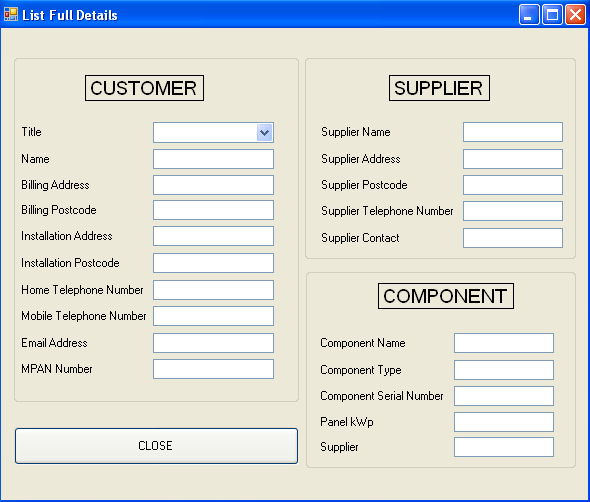
\includegraphics[scale=0.5]{frmListFullDetails_scrot}
	\makeatletter
\def\PY@reset{\let\PY@it=\relax \let\PY@bf=\relax%
    \let\PY@ul=\relax \let\PY@tc=\relax%
    \let\PY@bc=\relax \let\PY@ff=\relax}
\def\PY@tok#1{\csname PY@tok@#1\endcsname}
\def\PY@toks#1+{\ifx\relax#1\empty\else%
    \PY@tok{#1}\expandafter\PY@toks\fi}
\def\PY@do#1{\PY@bc{\PY@tc{\PY@ul{%
    \PY@it{\PY@bf{\PY@ff{#1}}}}}}}
\def\PY#1#2{\PY@reset\PY@toks#1+\relax+\PY@do{#2}}

\expandafter\def\csname PY@tok@gd\endcsname{\def\PY@tc##1{\textcolor[rgb]{0.63,0.00,0.00}{##1}}}
\expandafter\def\csname PY@tok@gu\endcsname{\let\PY@bf=\textbf\def\PY@tc##1{\textcolor[rgb]{0.50,0.00,0.50}{##1}}}
\expandafter\def\csname PY@tok@gt\endcsname{\def\PY@tc##1{\textcolor[rgb]{0.00,0.25,0.82}{##1}}}
\expandafter\def\csname PY@tok@gs\endcsname{\let\PY@bf=\textbf}
\expandafter\def\csname PY@tok@gr\endcsname{\def\PY@tc##1{\textcolor[rgb]{1.00,0.00,0.00}{##1}}}
\expandafter\def\csname PY@tok@cm\endcsname{\let\PY@it=\textit\def\PY@tc##1{\textcolor[rgb]{0.25,0.50,0.50}{##1}}}
\expandafter\def\csname PY@tok@vg\endcsname{\def\PY@tc##1{\textcolor[rgb]{0.10,0.09,0.49}{##1}}}
\expandafter\def\csname PY@tok@m\endcsname{\def\PY@tc##1{\textcolor[rgb]{0.40,0.40,0.40}{##1}}}
\expandafter\def\csname PY@tok@mh\endcsname{\def\PY@tc##1{\textcolor[rgb]{0.40,0.40,0.40}{##1}}}
\expandafter\def\csname PY@tok@go\endcsname{\def\PY@tc##1{\textcolor[rgb]{0.50,0.50,0.50}{##1}}}
\expandafter\def\csname PY@tok@ge\endcsname{\let\PY@it=\textit}
\expandafter\def\csname PY@tok@vc\endcsname{\def\PY@tc##1{\textcolor[rgb]{0.10,0.09,0.49}{##1}}}
\expandafter\def\csname PY@tok@il\endcsname{\def\PY@tc##1{\textcolor[rgb]{0.40,0.40,0.40}{##1}}}
\expandafter\def\csname PY@tok@cs\endcsname{\let\PY@it=\textit\def\PY@tc##1{\textcolor[rgb]{0.25,0.50,0.50}{##1}}}
\expandafter\def\csname PY@tok@cp\endcsname{\def\PY@tc##1{\textcolor[rgb]{0.74,0.48,0.00}{##1}}}
\expandafter\def\csname PY@tok@gi\endcsname{\def\PY@tc##1{\textcolor[rgb]{0.00,0.63,0.00}{##1}}}
\expandafter\def\csname PY@tok@gh\endcsname{\let\PY@bf=\textbf\def\PY@tc##1{\textcolor[rgb]{0.00,0.00,0.50}{##1}}}
\expandafter\def\csname PY@tok@ni\endcsname{\let\PY@bf=\textbf\def\PY@tc##1{\textcolor[rgb]{0.60,0.60,0.60}{##1}}}
\expandafter\def\csname PY@tok@nl\endcsname{\def\PY@tc##1{\textcolor[rgb]{0.63,0.63,0.00}{##1}}}
\expandafter\def\csname PY@tok@nn\endcsname{\let\PY@bf=\textbf\def\PY@tc##1{\textcolor[rgb]{0.00,0.00,1.00}{##1}}}
\expandafter\def\csname PY@tok@no\endcsname{\def\PY@tc##1{\textcolor[rgb]{0.53,0.00,0.00}{##1}}}
\expandafter\def\csname PY@tok@na\endcsname{\def\PY@tc##1{\textcolor[rgb]{0.49,0.56,0.16}{##1}}}
\expandafter\def\csname PY@tok@nb\endcsname{\def\PY@tc##1{\textcolor[rgb]{0.00,0.50,0.00}{##1}}}
\expandafter\def\csname PY@tok@nc\endcsname{\let\PY@bf=\textbf\def\PY@tc##1{\textcolor[rgb]{0.00,0.00,1.00}{##1}}}
\expandafter\def\csname PY@tok@nd\endcsname{\def\PY@tc##1{\textcolor[rgb]{0.67,0.13,1.00}{##1}}}
\expandafter\def\csname PY@tok@ne\endcsname{\let\PY@bf=\textbf\def\PY@tc##1{\textcolor[rgb]{0.82,0.25,0.23}{##1}}}
\expandafter\def\csname PY@tok@nf\endcsname{\def\PY@tc##1{\textcolor[rgb]{0.00,0.00,1.00}{##1}}}
\expandafter\def\csname PY@tok@si\endcsname{\let\PY@bf=\textbf\def\PY@tc##1{\textcolor[rgb]{0.73,0.40,0.53}{##1}}}
\expandafter\def\csname PY@tok@s2\endcsname{\def\PY@tc##1{\textcolor[rgb]{0.73,0.13,0.13}{##1}}}
\expandafter\def\csname PY@tok@vi\endcsname{\def\PY@tc##1{\textcolor[rgb]{0.10,0.09,0.49}{##1}}}
\expandafter\def\csname PY@tok@nt\endcsname{\let\PY@bf=\textbf\def\PY@tc##1{\textcolor[rgb]{0.00,0.50,0.00}{##1}}}
\expandafter\def\csname PY@tok@nv\endcsname{\def\PY@tc##1{\textcolor[rgb]{0.10,0.09,0.49}{##1}}}
\expandafter\def\csname PY@tok@s1\endcsname{\def\PY@tc##1{\textcolor[rgb]{0.73,0.13,0.13}{##1}}}
\expandafter\def\csname PY@tok@sh\endcsname{\def\PY@tc##1{\textcolor[rgb]{0.73,0.13,0.13}{##1}}}
\expandafter\def\csname PY@tok@sc\endcsname{\def\PY@tc##1{\textcolor[rgb]{0.73,0.13,0.13}{##1}}}
\expandafter\def\csname PY@tok@sx\endcsname{\def\PY@tc##1{\textcolor[rgb]{0.00,0.50,0.00}{##1}}}
\expandafter\def\csname PY@tok@bp\endcsname{\def\PY@tc##1{\textcolor[rgb]{0.00,0.50,0.00}{##1}}}
\expandafter\def\csname PY@tok@c1\endcsname{\let\PY@it=\textit\def\PY@tc##1{\textcolor[rgb]{0.25,0.50,0.50}{##1}}}
\expandafter\def\csname PY@tok@kc\endcsname{\let\PY@bf=\textbf\def\PY@tc##1{\textcolor[rgb]{0.00,0.50,0.00}{##1}}}
\expandafter\def\csname PY@tok@c\endcsname{\let\PY@it=\textit\def\PY@tc##1{\textcolor[rgb]{0.25,0.50,0.50}{##1}}}
\expandafter\def\csname PY@tok@mf\endcsname{\def\PY@tc##1{\textcolor[rgb]{0.40,0.40,0.40}{##1}}}
\expandafter\def\csname PY@tok@err\endcsname{\def\PY@bc##1{\setlength{\fboxsep}{0pt}\fcolorbox[rgb]{1.00,0.00,0.00}{1,1,1}{\strut ##1}}}
\expandafter\def\csname PY@tok@kd\endcsname{\let\PY@bf=\textbf\def\PY@tc##1{\textcolor[rgb]{0.00,0.50,0.00}{##1}}}
\expandafter\def\csname PY@tok@ss\endcsname{\def\PY@tc##1{\textcolor[rgb]{0.10,0.09,0.49}{##1}}}
\expandafter\def\csname PY@tok@sr\endcsname{\def\PY@tc##1{\textcolor[rgb]{0.73,0.40,0.53}{##1}}}
\expandafter\def\csname PY@tok@mo\endcsname{\def\PY@tc##1{\textcolor[rgb]{0.40,0.40,0.40}{##1}}}
\expandafter\def\csname PY@tok@kn\endcsname{\let\PY@bf=\textbf\def\PY@tc##1{\textcolor[rgb]{0.00,0.50,0.00}{##1}}}
\expandafter\def\csname PY@tok@mi\endcsname{\def\PY@tc##1{\textcolor[rgb]{0.40,0.40,0.40}{##1}}}
\expandafter\def\csname PY@tok@gp\endcsname{\let\PY@bf=\textbf\def\PY@tc##1{\textcolor[rgb]{0.00,0.00,0.50}{##1}}}
\expandafter\def\csname PY@tok@o\endcsname{\def\PY@tc##1{\textcolor[rgb]{0.40,0.40,0.40}{##1}}}
\expandafter\def\csname PY@tok@kr\endcsname{\let\PY@bf=\textbf\def\PY@tc##1{\textcolor[rgb]{0.00,0.50,0.00}{##1}}}
\expandafter\def\csname PY@tok@s\endcsname{\def\PY@tc##1{\textcolor[rgb]{0.73,0.13,0.13}{##1}}}
\expandafter\def\csname PY@tok@kp\endcsname{\def\PY@tc##1{\textcolor[rgb]{0.00,0.50,0.00}{##1}}}
\expandafter\def\csname PY@tok@w\endcsname{\def\PY@tc##1{\textcolor[rgb]{0.73,0.73,0.73}{##1}}}
\expandafter\def\csname PY@tok@kt\endcsname{\def\PY@tc##1{\textcolor[rgb]{0.69,0.00,0.25}{##1}}}
\expandafter\def\csname PY@tok@ow\endcsname{\let\PY@bf=\textbf\def\PY@tc##1{\textcolor[rgb]{0.67,0.13,1.00}{##1}}}
\expandafter\def\csname PY@tok@sb\endcsname{\def\PY@tc##1{\textcolor[rgb]{0.73,0.13,0.13}{##1}}}
\expandafter\def\csname PY@tok@k\endcsname{\let\PY@bf=\textbf\def\PY@tc##1{\textcolor[rgb]{0.00,0.50,0.00}{##1}}}
\expandafter\def\csname PY@tok@se\endcsname{\let\PY@bf=\textbf\def\PY@tc##1{\textcolor[rgb]{0.73,0.40,0.13}{##1}}}
\expandafter\def\csname PY@tok@sd\endcsname{\let\PY@it=\textit\def\PY@tc##1{\textcolor[rgb]{0.73,0.13,0.13}{##1}}}

\def\PYZbs{\char`\\}
\def\PYZus{\char`\_}
\def\PYZob{\char`\{}
\def\PYZcb{\char`\}}
\def\PYZca{\char`\^}
\def\PYZam{\char`\&}
\def\PYZlt{\char`\<}
\def\PYZgt{\char`\>}
\def\PYZsh{\char`\#}
\def\PYZpc{\char`\%}
\def\PYZdl{\char`\$}
\def\PYZti{\char`\~}
% for compatibility with earlier versions
\def\PYZat{@}
\def\PYZlb{[}
\def\PYZrb{]}
\makeatother

\begin{Verbatim}[commandchars=\\\{\}]
\PY{err}{�}\PY{err}{�}\PY{err}{�}\PY{k}{Imports} \PY{n+nn}{System.Data}
\PY{k}{Imports} \PY{n+nn}{System.Data.OleDb}

\PY{k}{Public} \PY{k}{Class} \PY{n+nc}{frmListFullDetails}
    \PY{k}{Public} \PY{n}{accConnection} \PY{o+ow}{As} \PY{k}{New} \PY{n}{OleDbConnection}

    \PY{k}{Private} \PY{k}{Sub} \PY{n+nf}{frmListFullDetails\PYZus{}Load}\PY{p}{(}\PY{k}{ByVal} \PY{n}{sender} \PY{o+ow}{As} \PY{n}{System}\PY{p}{.}\PY{n}{Object}\PY{p}{,} \PY{n}{\PYZus{}}
                                        \PY{k}{ByVal} \PY{n}{e} \PY{o+ow}{As} \PY{n}{System}\PY{p}{.}\PY{n}{EventArgs}\PY{p}{)} \PY{k}{Handles} \PY{k}{MyBase}\PY{p}{.}\PY{n}{Load}
        \PY{c}{'Reopen the database connection if it isn't open already.}
        \PY{k}{If} \PY{n}{frmLoginForm}\PY{p}{.}\PY{n}{accConnection}\PY{p}{.}\PY{n}{State} \PY{o}{\PYZlt{}\PYZgt{}} \PY{n}{ConnectionState}\PY{p}{.}\PY{n}{Open} \PY{k}{Then}
            \PY{n}{frmLoginForm}\PY{p}{.}\PY{n}{accConnection}\PY{p}{.}\PY{n}{Open}\PY{p}{(}\PY{p}{)}
        \PY{k}{End} \PY{k}{If}

        \PY{c}{'Call different procedures depending on what the user selected.}
        \PY{k}{If} \PY{n}{frmList}\PY{p}{.}\PY{n}{cbtxtListOptions}\PY{p}{.}\PY{n}{SelectedItem} \PY{o}{=} \PY{l+s}{"}\PY{l+s}{Customers}\PY{l+s}{"} \PY{k}{Then}
            \PY{k}{Call} \PY{n}{PopulateCustInfo}\PY{p}{(}\PY{p}{)}
        \PY{k}{ElseIf} \PY{n}{frmList}\PY{p}{.}\PY{n}{cbtxtListOptions}\PY{p}{.}\PY{n}{SelectedItem} \PY{o}{=} \PY{l+s}{"}\PY{l+s}{Suppliers}\PY{l+s}{"} \PY{k}{Then}
            \PY{k}{Call} \PY{n}{PopulateSuppInfo}\PY{p}{(}\PY{p}{)}
        \PY{k}{ElseIf} \PY{n}{frmList}\PY{p}{.}\PY{n}{cbtxtListOptions}\PY{p}{.}\PY{n}{SelectedItem} \PY{o}{=} \PY{l+s}{"}\PY{l+s}{Components}\PY{l+s}{"} \PY{k}{Then}
            \PY{k}{Call} \PY{n}{PopulateCompInfo}\PY{p}{(}\PY{p}{)}
        \PY{k}{End} \PY{k}{If}
    \PY{k}{End} \PY{k}{Sub}

    \PY{k}{Private} \PY{k}{Sub} \PY{n+nf}{PopulateCustInfo}\PY{p}{(}\PY{p}{)}

        \PY{n}{accConnection} \PY{o}{=} \PY{n}{frmLoginForm}\PY{p}{.}\PY{n}{accConnection}
        \PY{c}{'Input customer name from the other form and attribute it to CTN.}
        \PY{k}{Dim} \PY{n}{ctn} \PY{o+ow}{As} \PY{k+kt}{String} \PY{o}{=} \PY{n}{frmList}\PY{p}{.}\PY{n}{lbList}\PY{p}{.}\PY{n}{SelectedItem} \PY{c}{'Customer name.}
        \PY{k}{Dim} \PY{n}{cmdString} \PY{o+ow}{As} \PY{k+kt}{String} \PY{o}{=} \PY{l+s}{"}\PY{l+s}{SELECT * FROM Customer WHERE cust\PYZus{}name = '}\PY{l+s}{"} \PY{o}{\PYZam{}} \PY{n}{ctn} \PY{o}{\PYZam{}} \PY{l+s}{"}\PY{l+s}{'}\PY{l+s}{"}
        \PY{k}{Dim} \PY{n}{accCommand} \PY{o+ow}{As} \PY{k}{New} \PY{n}{OleDbCommand}
        \PY{k}{Dim} \PY{n}{da} \PY{o+ow}{As} \PY{k}{New} \PY{n}{OleDbDataAdapter}\PY{p}{(}\PY{n}{cmdString}\PY{p}{,} \PY{n}{accConnection}\PY{p}{)}
        \PY{k}{Dim} \PY{n}{ds} \PY{o+ow}{As} \PY{k}{New} \PY{n}{DataSet}

        \PY{n}{da}\PY{p}{.}\PY{n}{Fill}\PY{p}{(}\PY{n}{ds}\PY{p}{,} \PY{l+s}{"}\PY{l+s}{Customer}\PY{l+s}{"}\PY{p}{)}

        \PY{k}{Dim} \PY{n}{dt} \PY{o+ow}{As} \PY{n}{DataTable} \PY{o}{=} \PY{n}{ds}\PY{p}{.}\PY{n}{Tables}\PY{p}{(}\PY{l+m+mi}{0}\PY{p}{)}
        \PY{c}{'Dim dr As DataRow \PYZlt{}- This is redundant - it does not do anything.}

        \PY{c}{'Populate the textboxes in the form with existing customer details.}
        \PY{c}{'All the customer data text boxes are read-only to avoid data error:}
        \PY{c}{'to edit those, edit the customer details directly, then come back.}

        \PY{c}{'Populate the customer name textbox with the customer name}
        \PY{c}{'from the other form, before getting info from db about others.}

        \PY{c}{'An example of my variable naming here:}
        \PY{c}{'The variable 'txtldcn' = textbox listdetails custname.}
        \PY{n}{txtldctn}\PY{p}{.}\PY{n}{Text} \PY{o}{=} \PY{n}{ctn}
        \PY{k}{If} \PY{n}{ds}\PY{p}{.}\PY{n}{Tables}\PY{p}{(}\PY{l+m+mi}{0}\PY{p}{)}\PY{p}{.}\PY{n}{Rows}\PY{p}{.}\PY{n}{Count} \PY{o}{\PYZlt{}\PYZgt{}} \PY{l+m+mi}{0} \PY{k}{Then}
            \PY{n}{cbldctt}\PY{p}{.}\PY{n}{Text} \PY{o}{=} \PY{n}{ds}\PY{p}{.}\PY{n}{Tables}\PY{p}{(}\PY{l+m+mi}{0}\PY{p}{)}\PY{p}{.}\PY{n}{Rows}\PY{p}{(}\PY{l+m+mi}{0}\PY{p}{)}\PY{p}{.}\PY{n}{Item}\PY{p}{(}\PY{l+s}{"}\PY{l+s}{cust\PYZus{}title}\PY{l+s}{"}\PY{p}{)}
            \PY{n}{txtldctba}\PY{p}{.}\PY{n}{Text} \PY{o}{=} \PY{n}{ds}\PY{p}{.}\PY{n}{Tables}\PY{p}{(}\PY{l+m+mi}{0}\PY{p}{)}\PY{p}{.}\PY{n}{Rows}\PY{p}{(}\PY{l+m+mi}{0}\PY{p}{)}\PY{p}{.}\PY{n}{Item}\PY{p}{(}\PY{l+s}{"}\PY{l+s}{cust\PYZus{}billaddress}\PY{l+s}{"}\PY{p}{)}
            \PY{n}{txtldctbp}\PY{p}{.}\PY{n}{Text} \PY{o}{=} \PY{n}{ds}\PY{p}{.}\PY{n}{Tables}\PY{p}{(}\PY{l+m+mi}{0}\PY{p}{)}\PY{p}{.}\PY{n}{Rows}\PY{p}{(}\PY{l+m+mi}{0}\PY{p}{)}\PY{p}{.}\PY{n}{Item}\PY{p}{(}\PY{l+s}{"}\PY{l+s}{cust\PYZus{}billpostcode}\PY{l+s}{"}\PY{p}{)}
            \PY{n}{txtldctia}\PY{p}{.}\PY{n}{Text} \PY{o}{=} \PY{n}{ds}\PY{p}{.}\PY{n}{Tables}\PY{p}{(}\PY{l+m+mi}{0}\PY{p}{)}\PY{p}{.}\PY{n}{Rows}\PY{p}{(}\PY{l+m+mi}{0}\PY{p}{)}\PY{p}{.}\PY{n}{Item}\PY{p}{(}\PY{l+s}{"}\PY{l+s}{cust\PYZus{}instaddress}\PY{l+s}{"}\PY{p}{)}
            \PY{n}{txtldctip}\PY{p}{.}\PY{n}{Text} \PY{o}{=} \PY{n}{ds}\PY{p}{.}\PY{n}{Tables}\PY{p}{(}\PY{l+m+mi}{0}\PY{p}{)}\PY{p}{.}\PY{n}{Rows}\PY{p}{(}\PY{l+m+mi}{0}\PY{p}{)}\PY{p}{.}\PY{n}{Item}\PY{p}{(}\PY{l+s}{"}\PY{l+s}{cust\PYZus{}instpostcode}\PY{l+s}{"}\PY{p}{)}
            \PY{n}{txtldcthtn}\PY{p}{.}\PY{n}{Text} \PY{o}{=} \PY{n}{ds}\PY{p}{.}\PY{n}{Tables}\PY{p}{(}\PY{l+m+mi}{0}\PY{p}{)}\PY{p}{.}\PY{n}{Rows}\PY{p}{(}\PY{l+m+mi}{0}\PY{p}{)}\PY{p}{.}\PY{n}{Item}\PY{p}{(}\PY{l+s}{"}\PY{l+s}{cust\PYZus{}hometelno}\PY{l+s}{"}\PY{p}{)}
            \PY{n}{txtldctmtn}\PY{p}{.}\PY{n}{Text} \PY{o}{=} \PY{n}{ds}\PY{p}{.}\PY{n}{Tables}\PY{p}{(}\PY{l+m+mi}{0}\PY{p}{)}\PY{p}{.}\PY{n}{Rows}\PY{p}{(}\PY{l+m+mi}{0}\PY{p}{)}\PY{p}{.}\PY{n}{Item}\PY{p}{(}\PY{l+s}{"}\PY{l+s}{cust\PYZus{}mobtelno}\PY{l+s}{"}\PY{p}{)}
            \PY{n}{txtldctea}\PY{p}{.}\PY{n}{Text} \PY{o}{=} \PY{n}{ds}\PY{p}{.}\PY{n}{Tables}\PY{p}{(}\PY{l+m+mi}{0}\PY{p}{)}\PY{p}{.}\PY{n}{Rows}\PY{p}{(}\PY{l+m+mi}{0}\PY{p}{)}\PY{p}{.}\PY{n}{Item}\PY{p}{(}\PY{l+s}{"}\PY{l+s}{cust\PYZus{}email}\PY{l+s}{"}\PY{p}{)}
            \PY{n}{txtldctmpan}\PY{p}{.}\PY{n}{Text} \PY{o}{=} \PY{n}{ds}\PY{p}{.}\PY{n}{Tables}\PY{p}{(}\PY{l+m+mi}{0}\PY{p}{)}\PY{p}{.}\PY{n}{Rows}\PY{p}{(}\PY{l+m+mi}{0}\PY{p}{)}\PY{p}{.}\PY{n}{Item}\PY{p}{(}\PY{l+s}{"}\PY{l+s}{cust\PYZus{}mpan}\PY{l+s}{"}\PY{p}{)}
        \PY{k}{End} \PY{k}{If}

        \PY{n}{accCommand}\PY{p}{.}\PY{n}{Connection} \PY{o}{=} \PY{n}{frmLoginForm}\PY{p}{.}\PY{n}{accConnection}
        \PY{n}{accCommand}\PY{p}{.}\PY{n}{CommandType} \PY{o}{=} \PY{n}{CommandType}\PY{p}{.}\PY{n}{Text}
        \PY{n}{accCommand}\PY{p}{.}\PY{n}{CommandText} \PY{o}{=} \PY{n}{cmdString}
    \PY{k}{End} \PY{k}{Sub}

    \PY{k}{Private} \PY{k}{Sub} \PY{n+nf}{PopulateSuppInfo}\PY{p}{(}\PY{p}{)}

        \PY{n}{accConnection} \PY{o}{=} \PY{n}{frmLoginForm}\PY{p}{.}\PY{n}{accConnection}
        \PY{c}{'Input supplier name from the other form and attribute it to SPN.}
        \PY{k}{Dim} \PY{n}{spn} \PY{o+ow}{As} \PY{k+kt}{String} \PY{o}{=} \PY{n}{frmList}\PY{p}{.}\PY{n}{lbList}\PY{p}{.}\PY{n}{SelectedItem} \PY{c}{'Supplier name.}
        \PY{k}{Dim} \PY{n}{cmdString} \PY{o+ow}{As} \PY{k+kt}{String} \PY{o}{=} \PY{l+s}{"}\PY{l+s}{SELECT * FROM Supplier WHERE supp\PYZus{}name = '}\PY{l+s}{"} \PY{o}{\PYZam{}} \PY{n}{spn} \PY{o}{\PYZam{}} \PY{l+s}{"}\PY{l+s}{'}\PY{l+s}{"}
        \PY{k}{Dim} \PY{n}{accCommand} \PY{o+ow}{As} \PY{k}{New} \PY{n}{OleDbCommand}
        \PY{k}{Dim} \PY{n}{da} \PY{o+ow}{As} \PY{k}{New} \PY{n}{OleDbDataAdapter}\PY{p}{(}\PY{n}{cmdString}\PY{p}{,} \PY{n}{accConnection}\PY{p}{)}
        \PY{k}{Dim} \PY{n}{ds} \PY{o+ow}{As} \PY{k}{New} \PY{n}{DataSet}

        \PY{n}{da}\PY{p}{.}\PY{n}{Fill}\PY{p}{(}\PY{n}{ds}\PY{p}{,} \PY{l+s}{"}\PY{l+s}{Supplier}\PY{l+s}{"}\PY{p}{)}

        \PY{k}{Dim} \PY{n}{dt} \PY{o+ow}{As} \PY{n}{DataTable} \PY{o}{=} \PY{n}{ds}\PY{p}{.}\PY{n}{Tables}\PY{p}{(}\PY{l+m+mi}{0}\PY{p}{)}
        \PY{c}{'Dim dr As DataRow \PYZlt{}- This is redundant - it does not do anything.}

        \PY{c}{'Populate the textboxes in the form with existing supplier details.}
        \PY{c}{'All the supplier data text boxes are read-only to avoid data error:}
        \PY{c}{'to edit those, edit the supplier details directly, then come back.}

        \PY{c}{'Populate the supplier name textbox with the customer name}
        \PY{c}{'from the other form, before getting info from db about others.}

        \PY{c}{'An example of my variable naming here:}
        \PY{c}{'The variable 'txtldspn' = textbox listdetails suppname.}
        \PY{n}{txtldspn}\PY{p}{.}\PY{n}{Text} \PY{o}{=} \PY{n}{spn}
        \PY{k}{If} \PY{n}{ds}\PY{p}{.}\PY{n}{Tables}\PY{p}{(}\PY{l+m+mi}{0}\PY{p}{)}\PY{p}{.}\PY{n}{Rows}\PY{p}{.}\PY{n}{Count} \PY{o}{\PYZlt{}\PYZgt{}} \PY{l+m+mi}{0} \PY{k}{Then}
            \PY{n}{txtldspa}\PY{p}{.}\PY{n}{Text} \PY{o}{=} \PY{n}{ds}\PY{p}{.}\PY{n}{Tables}\PY{p}{(}\PY{l+m+mi}{0}\PY{p}{)}\PY{p}{.}\PY{n}{Rows}\PY{p}{(}\PY{l+m+mi}{0}\PY{p}{)}\PY{p}{.}\PY{n}{Item}\PY{p}{(}\PY{l+s}{"}\PY{l+s}{supp\PYZus{}address}\PY{l+s}{"}\PY{p}{)}
            \PY{n}{txtldspp}\PY{p}{.}\PY{n}{Text} \PY{o}{=} \PY{n}{ds}\PY{p}{.}\PY{n}{Tables}\PY{p}{(}\PY{l+m+mi}{0}\PY{p}{)}\PY{p}{.}\PY{n}{Rows}\PY{p}{(}\PY{l+m+mi}{0}\PY{p}{)}\PY{p}{.}\PY{n}{Item}\PY{p}{(}\PY{l+s}{"}\PY{l+s}{supp\PYZus{}postcode}\PY{l+s}{"}\PY{p}{)}
            \PY{n}{txtldsptn}\PY{p}{.}\PY{n}{Text} \PY{o}{=} \PY{n}{ds}\PY{p}{.}\PY{n}{Tables}\PY{p}{(}\PY{l+m+mi}{0}\PY{p}{)}\PY{p}{.}\PY{n}{Rows}\PY{p}{(}\PY{l+m+mi}{0}\PY{p}{)}\PY{p}{.}\PY{n}{Item}\PY{p}{(}\PY{l+s}{"}\PY{l+s}{supp\PYZus{}telno}\PY{l+s}{"}\PY{p}{)}
            \PY{n}{txtldspc}\PY{p}{.}\PY{n}{Text} \PY{o}{=} \PY{n}{ds}\PY{p}{.}\PY{n}{Tables}\PY{p}{(}\PY{l+m+mi}{0}\PY{p}{)}\PY{p}{.}\PY{n}{Rows}\PY{p}{(}\PY{l+m+mi}{0}\PY{p}{)}\PY{p}{.}\PY{n}{Item}\PY{p}{(}\PY{l+s}{"}\PY{l+s}{supp\PYZus{}contactname}\PY{l+s}{"}\PY{p}{)}
        \PY{k}{End} \PY{k}{If}

        \PY{n}{accCommand}\PY{p}{.}\PY{n}{Connection} \PY{o}{=} \PY{n}{frmLoginForm}\PY{p}{.}\PY{n}{accConnection}
        \PY{n}{accCommand}\PY{p}{.}\PY{n}{CommandType} \PY{o}{=} \PY{n}{CommandType}\PY{p}{.}\PY{n}{Text}
        \PY{n}{accCommand}\PY{p}{.}\PY{n}{CommandText} \PY{o}{=} \PY{n}{cmdString}

    \PY{k}{End} \PY{k}{Sub}

    \PY{k}{Private} \PY{k}{Sub} \PY{n+nf}{PopulateCompInfo}\PY{p}{(}\PY{p}{)}

        \PY{n}{accConnection} \PY{o}{=} \PY{n}{frmLoginForm}\PY{p}{.}\PY{n}{accConnection}
        \PY{c}{'Input component name from the other form and attribute it to CPN.}
        \PY{k}{Dim} \PY{n}{cpn} \PY{o+ow}{As} \PY{k+kt}{String} \PY{o}{=} \PY{n}{frmList}\PY{p}{.}\PY{n}{lbList}\PY{p}{.}\PY{n}{SelectedItem} \PY{c}{'Component name.}
        \PY{k}{Dim} \PY{n}{cmdString} \PY{o+ow}{As} \PY{k+kt}{String} \PY{o}{=} \PY{l+s}{"}\PY{l+s}{SELECT * FROM Component WHERE comp\PYZus{}name = '}\PY{l+s}{"} \PY{o}{\PYZam{}} \PY{n}{cpn} \PY{o}{\PYZam{}} \PY{l+s}{"}\PY{l+s}{'}\PY{l+s}{"}

        \PY{k}{Dim} \PY{n}{accCommand} \PY{o+ow}{As} \PY{k}{New} \PY{n}{OleDbCommand}
        \PY{k}{Dim} \PY{n}{da} \PY{o+ow}{As} \PY{k}{New} \PY{n}{OleDbDataAdapter}\PY{p}{(}\PY{n}{cmdString}\PY{p}{,} \PY{n}{accConnection}\PY{p}{)}
        \PY{k}{Dim} \PY{n}{ds} \PY{o+ow}{As} \PY{k}{New} \PY{n}{DataSet}

        \PY{n}{da}\PY{p}{.}\PY{n}{Fill}\PY{p}{(}\PY{n}{ds}\PY{p}{,} \PY{l+s}{"}\PY{l+s}{Component}\PY{l+s}{"}\PY{p}{)}

        \PY{k}{Dim} \PY{n}{dt} \PY{o+ow}{As} \PY{n}{DataTable} \PY{o}{=} \PY{n}{ds}\PY{p}{.}\PY{n}{Tables}\PY{p}{(}\PY{l+m+mi}{0}\PY{p}{)}
        \PY{c}{'Dim dr As DataRow \PYZlt{}- This is redundant - it does not do anything.}

        \PY{k}{Dim} \PY{n}{compsupplierval} \PY{o+ow}{As} \PY{k+kt}{Integer} \PY{o}{=} \PY{l+m+mi}{0}

        \PY{c}{'Check if a supplier is selected.  Before this Try/Catch, the}
        \PY{c}{'program would crash due to no value at row 0 of the table.}
        \PY{k}{Try}
            \PY{n}{compsupplierval} \PY{o}{=} \PY{n}{ds}\PY{p}{.}\PY{n}{Tables}\PY{p}{(}\PY{l+m+mi}{0}\PY{p}{)}\PY{p}{.}\PY{n}{Rows}\PY{p}{(}\PY{l+m+mi}{0}\PY{p}{)}\PY{p}{.}\PY{n}{Item}\PY{p}{(}\PY{l+s}{"}\PY{l+s}{comp\PYZus{}supplier}\PY{l+s}{"}\PY{p}{)}
        \PY{k}{Catch}
        \PY{k}{End} \PY{k}{Try}

        \PY{k}{Dim} \PY{n}{csuppv} \PY{o+ow}{As} \PY{k+kt}{Integer} \PY{o}{=} \PY{n}{compsupplierval}
        \PY{k}{Dim} \PY{n}{sn} \PY{o+ow}{As} \PY{k+kt}{String} \PY{o}{=} \PY{l+s}{"}\PY{l+s}{"} \PY{c}{'Supplier name, initially blank here.}

        \PY{c}{'Now call the List form's switching supplier ID function.}
        \PY{c}{'No point creating a near identical one if there exists the}
        \PY{c}{'ability of reusing code.}
        \PY{k}{Call} \PY{n}{frmList}\PY{p}{.}\PY{n}{SwitchSuppIDToName}\PY{p}{(}\PY{n}{csuppv}\PY{p}{,} \PY{n}{sn}\PY{p}{)}

        \PY{c}{'Populate the textboxes in the form with existing component details.}
        \PY{c}{'All the component data text boxes are read-only to avoid data error:}
        \PY{c}{'to edit those, edit the component details directly, then come back.}

        \PY{c}{'Populate the component name textbox with the customer name}
        \PY{c}{'from the other form, before getting info from db about others.}

        \PY{c}{'An example of my variable naming here:}
        \PY{c}{'The variable 'txtldcpn' = textbox listdetails compname.}
        \PY{n}{txtldcpn}\PY{p}{.}\PY{n}{Text} \PY{o}{=} \PY{n}{cpn}
        \PY{k}{If} \PY{n}{ds}\PY{p}{.}\PY{n}{Tables}\PY{p}{(}\PY{l+m+mi}{0}\PY{p}{)}\PY{p}{.}\PY{n}{Rows}\PY{p}{.}\PY{n}{Count} \PY{o}{\PYZlt{}\PYZgt{}} \PY{l+m+mi}{0} \PY{k}{Then}
            \PY{n}{txtldcpt}\PY{p}{.}\PY{n}{Text} \PY{o}{=} \PY{n}{ds}\PY{p}{.}\PY{n}{Tables}\PY{p}{(}\PY{l+m+mi}{0}\PY{p}{)}\PY{p}{.}\PY{n}{Rows}\PY{p}{(}\PY{l+m+mi}{0}\PY{p}{)}\PY{p}{.}\PY{n}{Item}\PY{p}{(}\PY{l+s}{"}\PY{l+s}{comp\PYZus{}type}\PY{l+s}{"}\PY{p}{)}
            \PY{n}{txtldcpsn}\PY{p}{.}\PY{n}{Text} \PY{o}{=} \PY{n}{ds}\PY{p}{.}\PY{n}{Tables}\PY{p}{(}\PY{l+m+mi}{0}\PY{p}{)}\PY{p}{.}\PY{n}{Rows}\PY{p}{(}\PY{l+m+mi}{0}\PY{p}{)}\PY{p}{.}\PY{n}{Item}\PY{p}{(}\PY{l+s}{"}\PY{l+s}{comp\PYZus{}serialno}\PY{l+s}{"}\PY{p}{)}
            \PY{c}{'Divide by 1000 to get the kilowatt for the user rather than}
            \PY{c}{'the watt value from the database.}
            \PY{n}{txtldcppkwp}\PY{p}{.}\PY{n}{Text} \PY{o}{=} \PY{n}{ds}\PY{p}{.}\PY{n}{Tables}\PY{p}{(}\PY{l+m+mi}{0}\PY{p}{)}\PY{p}{.}\PY{n}{Rows}\PY{p}{(}\PY{l+m+mi}{0}\PY{p}{)}\PY{p}{.}\PY{n}{Item}\PY{p}{(}\PY{l+s}{"}\PY{l+s}{comp\PYZus{}panelwp}\PY{l+s}{"}\PY{p}{)} \PY{o}{/} \PY{l+m+mi}{1000}
            \PY{n}{txtldcpspn}\PY{p}{.}\PY{n}{Text} \PY{o}{=} \PY{n}{sn}
        \PY{k}{End} \PY{k}{If}

        \PY{n}{accCommand}\PY{p}{.}\PY{n}{Connection} \PY{o}{=} \PY{n}{frmLoginForm}\PY{p}{.}\PY{n}{accConnection}
        \PY{n}{accCommand}\PY{p}{.}\PY{n}{CommandType} \PY{o}{=} \PY{n}{CommandType}\PY{p}{.}\PY{n}{Text}
        \PY{n}{accCommand}\PY{p}{.}\PY{n}{CommandText} \PY{o}{=} \PY{n}{cmdString}
    \PY{k}{End} \PY{k}{Sub}

    \PY{k}{Private} \PY{k}{Sub} \PY{n+nf}{btnClose\PYZus{}Click}\PY{p}{(}\PY{k}{ByVal} \PY{n}{sender} \PY{o+ow}{As} \PY{n}{System}\PY{p}{.}\PY{n}{Object}\PY{p}{,} \PY{n}{\PYZus{}}
                               \PY{k}{ByVal} \PY{n}{e} \PY{o+ow}{As} \PY{n}{System}\PY{p}{.}\PY{n}{EventArgs}\PY{p}{)} \PY{k}{Handles} \PY{n}{btnClose}\PY{p}{.}\PY{n}{Click}
        \PY{n}{frmList}\PY{p}{.}\PY{n}{Show}\PY{p}{(}\PY{p}{)}
        \PY{k}{Me}\PY{p}{.}\PY{n}{Close}\PY{p}{(}\PY{p}{)}
    \PY{k}{End} \PY{k}{Sub}

\PY{k}{End} \PY{k}{Class}
\end{Verbatim}
	
\subsection{frmReportMenu}
	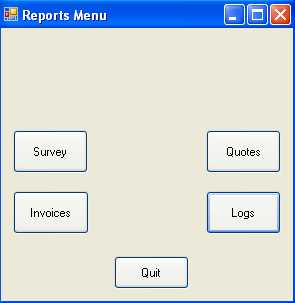
\includegraphics[scale=0.5]{frmReportMenu_scrot}
	\makeatletter
\def\PY@reset{\let\PY@it=\relax \let\PY@bf=\relax%
    \let\PY@ul=\relax \let\PY@tc=\relax%
    \let\PY@bc=\relax \let\PY@ff=\relax}
\def\PY@tok#1{\csname PY@tok@#1\endcsname}
\def\PY@toks#1+{\ifx\relax#1\empty\else%
    \PY@tok{#1}\expandafter\PY@toks\fi}
\def\PY@do#1{\PY@bc{\PY@tc{\PY@ul{%
    \PY@it{\PY@bf{\PY@ff{#1}}}}}}}
\def\PY#1#2{\PY@reset\PY@toks#1+\relax+\PY@do{#2}}

\expandafter\def\csname PY@tok@gd\endcsname{\def\PY@tc##1{\textcolor[rgb]{0.63,0.00,0.00}{##1}}}
\expandafter\def\csname PY@tok@gu\endcsname{\let\PY@bf=\textbf\def\PY@tc##1{\textcolor[rgb]{0.50,0.00,0.50}{##1}}}
\expandafter\def\csname PY@tok@gt\endcsname{\def\PY@tc##1{\textcolor[rgb]{0.00,0.25,0.82}{##1}}}
\expandafter\def\csname PY@tok@gs\endcsname{\let\PY@bf=\textbf}
\expandafter\def\csname PY@tok@gr\endcsname{\def\PY@tc##1{\textcolor[rgb]{1.00,0.00,0.00}{##1}}}
\expandafter\def\csname PY@tok@cm\endcsname{\let\PY@it=\textit\def\PY@tc##1{\textcolor[rgb]{0.25,0.50,0.50}{##1}}}
\expandafter\def\csname PY@tok@vg\endcsname{\def\PY@tc##1{\textcolor[rgb]{0.10,0.09,0.49}{##1}}}
\expandafter\def\csname PY@tok@m\endcsname{\def\PY@tc##1{\textcolor[rgb]{0.40,0.40,0.40}{##1}}}
\expandafter\def\csname PY@tok@mh\endcsname{\def\PY@tc##1{\textcolor[rgb]{0.40,0.40,0.40}{##1}}}
\expandafter\def\csname PY@tok@go\endcsname{\def\PY@tc##1{\textcolor[rgb]{0.50,0.50,0.50}{##1}}}
\expandafter\def\csname PY@tok@ge\endcsname{\let\PY@it=\textit}
\expandafter\def\csname PY@tok@vc\endcsname{\def\PY@tc##1{\textcolor[rgb]{0.10,0.09,0.49}{##1}}}
\expandafter\def\csname PY@tok@il\endcsname{\def\PY@tc##1{\textcolor[rgb]{0.40,0.40,0.40}{##1}}}
\expandafter\def\csname PY@tok@cs\endcsname{\let\PY@it=\textit\def\PY@tc##1{\textcolor[rgb]{0.25,0.50,0.50}{##1}}}
\expandafter\def\csname PY@tok@cp\endcsname{\def\PY@tc##1{\textcolor[rgb]{0.74,0.48,0.00}{##1}}}
\expandafter\def\csname PY@tok@gi\endcsname{\def\PY@tc##1{\textcolor[rgb]{0.00,0.63,0.00}{##1}}}
\expandafter\def\csname PY@tok@gh\endcsname{\let\PY@bf=\textbf\def\PY@tc##1{\textcolor[rgb]{0.00,0.00,0.50}{##1}}}
\expandafter\def\csname PY@tok@ni\endcsname{\let\PY@bf=\textbf\def\PY@tc##1{\textcolor[rgb]{0.60,0.60,0.60}{##1}}}
\expandafter\def\csname PY@tok@nl\endcsname{\def\PY@tc##1{\textcolor[rgb]{0.63,0.63,0.00}{##1}}}
\expandafter\def\csname PY@tok@nn\endcsname{\let\PY@bf=\textbf\def\PY@tc##1{\textcolor[rgb]{0.00,0.00,1.00}{##1}}}
\expandafter\def\csname PY@tok@no\endcsname{\def\PY@tc##1{\textcolor[rgb]{0.53,0.00,0.00}{##1}}}
\expandafter\def\csname PY@tok@na\endcsname{\def\PY@tc##1{\textcolor[rgb]{0.49,0.56,0.16}{##1}}}
\expandafter\def\csname PY@tok@nb\endcsname{\def\PY@tc##1{\textcolor[rgb]{0.00,0.50,0.00}{##1}}}
\expandafter\def\csname PY@tok@nc\endcsname{\let\PY@bf=\textbf\def\PY@tc##1{\textcolor[rgb]{0.00,0.00,1.00}{##1}}}
\expandafter\def\csname PY@tok@nd\endcsname{\def\PY@tc##1{\textcolor[rgb]{0.67,0.13,1.00}{##1}}}
\expandafter\def\csname PY@tok@ne\endcsname{\let\PY@bf=\textbf\def\PY@tc##1{\textcolor[rgb]{0.82,0.25,0.23}{##1}}}
\expandafter\def\csname PY@tok@nf\endcsname{\def\PY@tc##1{\textcolor[rgb]{0.00,0.00,1.00}{##1}}}
\expandafter\def\csname PY@tok@si\endcsname{\let\PY@bf=\textbf\def\PY@tc##1{\textcolor[rgb]{0.73,0.40,0.53}{##1}}}
\expandafter\def\csname PY@tok@s2\endcsname{\def\PY@tc##1{\textcolor[rgb]{0.73,0.13,0.13}{##1}}}
\expandafter\def\csname PY@tok@vi\endcsname{\def\PY@tc##1{\textcolor[rgb]{0.10,0.09,0.49}{##1}}}
\expandafter\def\csname PY@tok@nt\endcsname{\let\PY@bf=\textbf\def\PY@tc##1{\textcolor[rgb]{0.00,0.50,0.00}{##1}}}
\expandafter\def\csname PY@tok@nv\endcsname{\def\PY@tc##1{\textcolor[rgb]{0.10,0.09,0.49}{##1}}}
\expandafter\def\csname PY@tok@s1\endcsname{\def\PY@tc##1{\textcolor[rgb]{0.73,0.13,0.13}{##1}}}
\expandafter\def\csname PY@tok@sh\endcsname{\def\PY@tc##1{\textcolor[rgb]{0.73,0.13,0.13}{##1}}}
\expandafter\def\csname PY@tok@sc\endcsname{\def\PY@tc##1{\textcolor[rgb]{0.73,0.13,0.13}{##1}}}
\expandafter\def\csname PY@tok@sx\endcsname{\def\PY@tc##1{\textcolor[rgb]{0.00,0.50,0.00}{##1}}}
\expandafter\def\csname PY@tok@bp\endcsname{\def\PY@tc##1{\textcolor[rgb]{0.00,0.50,0.00}{##1}}}
\expandafter\def\csname PY@tok@c1\endcsname{\let\PY@it=\textit\def\PY@tc##1{\textcolor[rgb]{0.25,0.50,0.50}{##1}}}
\expandafter\def\csname PY@tok@kc\endcsname{\let\PY@bf=\textbf\def\PY@tc##1{\textcolor[rgb]{0.00,0.50,0.00}{##1}}}
\expandafter\def\csname PY@tok@c\endcsname{\let\PY@it=\textit\def\PY@tc##1{\textcolor[rgb]{0.25,0.50,0.50}{##1}}}
\expandafter\def\csname PY@tok@mf\endcsname{\def\PY@tc##1{\textcolor[rgb]{0.40,0.40,0.40}{##1}}}
\expandafter\def\csname PY@tok@err\endcsname{\def\PY@bc##1{\setlength{\fboxsep}{0pt}\fcolorbox[rgb]{1.00,0.00,0.00}{1,1,1}{\strut ##1}}}
\expandafter\def\csname PY@tok@kd\endcsname{\let\PY@bf=\textbf\def\PY@tc##1{\textcolor[rgb]{0.00,0.50,0.00}{##1}}}
\expandafter\def\csname PY@tok@ss\endcsname{\def\PY@tc##1{\textcolor[rgb]{0.10,0.09,0.49}{##1}}}
\expandafter\def\csname PY@tok@sr\endcsname{\def\PY@tc##1{\textcolor[rgb]{0.73,0.40,0.53}{##1}}}
\expandafter\def\csname PY@tok@mo\endcsname{\def\PY@tc##1{\textcolor[rgb]{0.40,0.40,0.40}{##1}}}
\expandafter\def\csname PY@tok@kn\endcsname{\let\PY@bf=\textbf\def\PY@tc##1{\textcolor[rgb]{0.00,0.50,0.00}{##1}}}
\expandafter\def\csname PY@tok@mi\endcsname{\def\PY@tc##1{\textcolor[rgb]{0.40,0.40,0.40}{##1}}}
\expandafter\def\csname PY@tok@gp\endcsname{\let\PY@bf=\textbf\def\PY@tc##1{\textcolor[rgb]{0.00,0.00,0.50}{##1}}}
\expandafter\def\csname PY@tok@o\endcsname{\def\PY@tc##1{\textcolor[rgb]{0.40,0.40,0.40}{##1}}}
\expandafter\def\csname PY@tok@kr\endcsname{\let\PY@bf=\textbf\def\PY@tc##1{\textcolor[rgb]{0.00,0.50,0.00}{##1}}}
\expandafter\def\csname PY@tok@s\endcsname{\def\PY@tc##1{\textcolor[rgb]{0.73,0.13,0.13}{##1}}}
\expandafter\def\csname PY@tok@kp\endcsname{\def\PY@tc##1{\textcolor[rgb]{0.00,0.50,0.00}{##1}}}
\expandafter\def\csname PY@tok@w\endcsname{\def\PY@tc##1{\textcolor[rgb]{0.73,0.73,0.73}{##1}}}
\expandafter\def\csname PY@tok@kt\endcsname{\def\PY@tc##1{\textcolor[rgb]{0.69,0.00,0.25}{##1}}}
\expandafter\def\csname PY@tok@ow\endcsname{\let\PY@bf=\textbf\def\PY@tc##1{\textcolor[rgb]{0.67,0.13,1.00}{##1}}}
\expandafter\def\csname PY@tok@sb\endcsname{\def\PY@tc##1{\textcolor[rgb]{0.73,0.13,0.13}{##1}}}
\expandafter\def\csname PY@tok@k\endcsname{\let\PY@bf=\textbf\def\PY@tc##1{\textcolor[rgb]{0.00,0.50,0.00}{##1}}}
\expandafter\def\csname PY@tok@se\endcsname{\let\PY@bf=\textbf\def\PY@tc##1{\textcolor[rgb]{0.73,0.40,0.13}{##1}}}
\expandafter\def\csname PY@tok@sd\endcsname{\let\PY@it=\textit\def\PY@tc##1{\textcolor[rgb]{0.73,0.13,0.13}{##1}}}

\def\PYZbs{\char`\\}
\def\PYZus{\char`\_}
\def\PYZob{\char`\{}
\def\PYZcb{\char`\}}
\def\PYZca{\char`\^}
\def\PYZam{\char`\&}
\def\PYZlt{\char`\<}
\def\PYZgt{\char`\>}
\def\PYZsh{\char`\#}
\def\PYZpc{\char`\%}
\def\PYZdl{\char`\$}
\def\PYZti{\char`\~}
% for compatibility with earlier versions
\def\PYZat{@}
\def\PYZlb{[}
\def\PYZrb{]}
\makeatother

\begin{Verbatim}[commandchars=\\\{\}]
\PY{err}{�}\PY{err}{�}\PY{err}{�}\PY{k}{Public} \PY{k}{Class} \PY{n+nc}{frmReportMenu}

    \PY{k}{Private} \PY{k}{Sub} \PY{n+nf}{btnQuit\PYZus{}Click}\PY{p}{(}\PY{k}{ByVal} \PY{n}{sender} \PY{o+ow}{As} \PY{n}{System}\PY{p}{.}\PY{n}{Object}\PY{p}{,} \PY{n}{\PYZus{}}
                              \PY{k}{ByVal} \PY{n}{e} \PY{o+ow}{As} \PY{n}{System}\PY{p}{.}\PY{n}{EventArgs}\PY{p}{)} \PY{k}{Handles} \PY{n}{btnQuit}\PY{p}{.}\PY{n}{Click}
        \PY{c}{'On close, close this window and show the main menu.}
        \PY{k}{Me}\PY{p}{.}\PY{n}{Close}\PY{p}{(}\PY{p}{)}
        \PY{n}{frmMainMenu}\PY{p}{.}\PY{n}{Show}\PY{p}{(}\PY{p}{)}
    \PY{k}{End} \PY{k}{Sub}

    \PY{k}{Private} \PY{k}{Sub} \PY{n+nf}{btnQuotes\PYZus{}Click}\PY{p}{(}\PY{k}{ByVal} \PY{n}{sender} \PY{o+ow}{As} \PY{n}{System}\PY{p}{.}\PY{n}{Object}\PY{p}{,} \PY{n}{\PYZus{}}
                                \PY{k}{ByVal} \PY{n}{e} \PY{o+ow}{As} \PY{n}{System}\PY{p}{.}\PY{n}{EventArgs}\PY{p}{)} \PY{k}{Handles} \PY{n}{btnQuotes}\PY{p}{.}\PY{n}{Click}
        \PY{c}{'Show the quote form to the user, then hide this menu window.}
        \PY{n}{frmReportQuote}\PY{p}{.}\PY{n}{Show}\PY{p}{(}\PY{p}{)}
        \PY{k}{Me}\PY{p}{.}\PY{n}{Hide}\PY{p}{(}\PY{p}{)}
    \PY{k}{End} \PY{k}{Sub}

    \PY{k}{Private} \PY{k}{Sub} \PY{n+nf}{btnLogs\PYZus{}Click}\PY{p}{(}\PY{k}{ByVal} \PY{n}{sender} \PY{o+ow}{As} \PY{n}{System}\PY{p}{.}\PY{n}{Object}\PY{p}{,} \PY{n}{\PYZus{}}
                              \PY{k}{ByVal} \PY{n}{e} \PY{o+ow}{As} \PY{n}{System}\PY{p}{.}\PY{n}{EventArgs}\PY{p}{)} \PY{k}{Handles} \PY{n}{btnLogs}\PY{p}{.}\PY{n}{Click}
        \PY{c}{'Show the log form to the user, then hide this menu window.}
        \PY{n}{frmReportLog}\PY{p}{.}\PY{n}{Show}\PY{p}{(}\PY{p}{)}
        \PY{k}{Me}\PY{p}{.}\PY{n}{Hide}\PY{p}{(}\PY{p}{)}
    \PY{k}{End} \PY{k}{Sub}

    \PY{k}{Private} \PY{k}{Sub} \PY{n+nf}{btnInvoices\PYZus{}Click}\PY{p}{(}\PY{k}{ByVal} \PY{n}{sender} \PY{o+ow}{As} \PY{n}{System}\PY{p}{.}\PY{n}{Object}\PY{p}{,} \PY{n}{\PYZus{}}
                                  \PY{k}{ByVal} \PY{n}{e} \PY{o+ow}{As} \PY{n}{System}\PY{p}{.}\PY{n}{EventArgs}\PY{p}{)} \PY{k}{Handles} \PY{n}{btnInvoices}\PY{p}{.}\PY{n}{Click}
        \PY{c}{'Show the invoice form to the user, then hide this menu window.}
        \PY{n}{frmReportInvoice}\PY{p}{.}\PY{n}{Show}\PY{p}{(}\PY{p}{)}
        \PY{k}{Me}\PY{p}{.}\PY{n}{Hide}\PY{p}{(}\PY{p}{)}
    \PY{k}{End} \PY{k}{Sub}

    \PY{k}{Private} \PY{k}{Sub} \PY{n+nf}{btnSurvey\PYZus{}Click}\PY{p}{(}\PY{k}{ByVal} \PY{n}{sender} \PY{o+ow}{As} \PY{n}{System}\PY{p}{.}\PY{n}{Object}\PY{p}{,} \PY{n}{\PYZus{}}
                                \PY{k}{ByVal} \PY{n}{e} \PY{o+ow}{As} \PY{n}{System}\PY{p}{.}\PY{n}{EventArgs}\PY{p}{)} \PY{k}{Handles} \PY{n}{btnSurvey}\PY{p}{.}\PY{n}{Click}
        \PY{c}{'Show the survey form to the user, then hide this menu window.}
        \PY{n}{frmReportSurvey}\PY{p}{.}\PY{n}{Show}\PY{p}{(}\PY{p}{)}
        \PY{k}{Me}\PY{p}{.}\PY{n}{Hide}\PY{p}{(}\PY{p}{)}
    \PY{k}{End} \PY{k}{Sub}

\PY{k}{End} \PY{k}{Class}
\end{Verbatim}
	
\subsection{frmReportInvoice}
	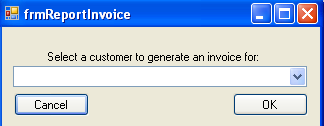
\includegraphics[scale=0.5]{frmReportInvoice_scrot}
	\makeatletter
\def\PY@reset{\let\PY@it=\relax \let\PY@bf=\relax%
    \let\PY@ul=\relax \let\PY@tc=\relax%
    \let\PY@bc=\relax \let\PY@ff=\relax}
\def\PY@tok#1{\csname PY@tok@#1\endcsname}
\def\PY@toks#1+{\ifx\relax#1\empty\else%
    \PY@tok{#1}\expandafter\PY@toks\fi}
\def\PY@do#1{\PY@bc{\PY@tc{\PY@ul{%
    \PY@it{\PY@bf{\PY@ff{#1}}}}}}}
\def\PY#1#2{\PY@reset\PY@toks#1+\relax+\PY@do{#2}}

\expandafter\def\csname PY@tok@gd\endcsname{\def\PY@tc##1{\textcolor[rgb]{0.63,0.00,0.00}{##1}}}
\expandafter\def\csname PY@tok@gu\endcsname{\let\PY@bf=\textbf\def\PY@tc##1{\textcolor[rgb]{0.50,0.00,0.50}{##1}}}
\expandafter\def\csname PY@tok@gt\endcsname{\def\PY@tc##1{\textcolor[rgb]{0.00,0.25,0.82}{##1}}}
\expandafter\def\csname PY@tok@gs\endcsname{\let\PY@bf=\textbf}
\expandafter\def\csname PY@tok@gr\endcsname{\def\PY@tc##1{\textcolor[rgb]{1.00,0.00,0.00}{##1}}}
\expandafter\def\csname PY@tok@cm\endcsname{\let\PY@it=\textit\def\PY@tc##1{\textcolor[rgb]{0.25,0.50,0.50}{##1}}}
\expandafter\def\csname PY@tok@vg\endcsname{\def\PY@tc##1{\textcolor[rgb]{0.10,0.09,0.49}{##1}}}
\expandafter\def\csname PY@tok@m\endcsname{\def\PY@tc##1{\textcolor[rgb]{0.40,0.40,0.40}{##1}}}
\expandafter\def\csname PY@tok@mh\endcsname{\def\PY@tc##1{\textcolor[rgb]{0.40,0.40,0.40}{##1}}}
\expandafter\def\csname PY@tok@go\endcsname{\def\PY@tc##1{\textcolor[rgb]{0.50,0.50,0.50}{##1}}}
\expandafter\def\csname PY@tok@ge\endcsname{\let\PY@it=\textit}
\expandafter\def\csname PY@tok@vc\endcsname{\def\PY@tc##1{\textcolor[rgb]{0.10,0.09,0.49}{##1}}}
\expandafter\def\csname PY@tok@il\endcsname{\def\PY@tc##1{\textcolor[rgb]{0.40,0.40,0.40}{##1}}}
\expandafter\def\csname PY@tok@cs\endcsname{\let\PY@it=\textit\def\PY@tc##1{\textcolor[rgb]{0.25,0.50,0.50}{##1}}}
\expandafter\def\csname PY@tok@cp\endcsname{\def\PY@tc##1{\textcolor[rgb]{0.74,0.48,0.00}{##1}}}
\expandafter\def\csname PY@tok@gi\endcsname{\def\PY@tc##1{\textcolor[rgb]{0.00,0.63,0.00}{##1}}}
\expandafter\def\csname PY@tok@gh\endcsname{\let\PY@bf=\textbf\def\PY@tc##1{\textcolor[rgb]{0.00,0.00,0.50}{##1}}}
\expandafter\def\csname PY@tok@ni\endcsname{\let\PY@bf=\textbf\def\PY@tc##1{\textcolor[rgb]{0.60,0.60,0.60}{##1}}}
\expandafter\def\csname PY@tok@nl\endcsname{\def\PY@tc##1{\textcolor[rgb]{0.63,0.63,0.00}{##1}}}
\expandafter\def\csname PY@tok@nn\endcsname{\let\PY@bf=\textbf\def\PY@tc##1{\textcolor[rgb]{0.00,0.00,1.00}{##1}}}
\expandafter\def\csname PY@tok@no\endcsname{\def\PY@tc##1{\textcolor[rgb]{0.53,0.00,0.00}{##1}}}
\expandafter\def\csname PY@tok@na\endcsname{\def\PY@tc##1{\textcolor[rgb]{0.49,0.56,0.16}{##1}}}
\expandafter\def\csname PY@tok@nb\endcsname{\def\PY@tc##1{\textcolor[rgb]{0.00,0.50,0.00}{##1}}}
\expandafter\def\csname PY@tok@nc\endcsname{\let\PY@bf=\textbf\def\PY@tc##1{\textcolor[rgb]{0.00,0.00,1.00}{##1}}}
\expandafter\def\csname PY@tok@nd\endcsname{\def\PY@tc##1{\textcolor[rgb]{0.67,0.13,1.00}{##1}}}
\expandafter\def\csname PY@tok@ne\endcsname{\let\PY@bf=\textbf\def\PY@tc##1{\textcolor[rgb]{0.82,0.25,0.23}{##1}}}
\expandafter\def\csname PY@tok@nf\endcsname{\def\PY@tc##1{\textcolor[rgb]{0.00,0.00,1.00}{##1}}}
\expandafter\def\csname PY@tok@si\endcsname{\let\PY@bf=\textbf\def\PY@tc##1{\textcolor[rgb]{0.73,0.40,0.53}{##1}}}
\expandafter\def\csname PY@tok@s2\endcsname{\def\PY@tc##1{\textcolor[rgb]{0.73,0.13,0.13}{##1}}}
\expandafter\def\csname PY@tok@vi\endcsname{\def\PY@tc##1{\textcolor[rgb]{0.10,0.09,0.49}{##1}}}
\expandafter\def\csname PY@tok@nt\endcsname{\let\PY@bf=\textbf\def\PY@tc##1{\textcolor[rgb]{0.00,0.50,0.00}{##1}}}
\expandafter\def\csname PY@tok@nv\endcsname{\def\PY@tc##1{\textcolor[rgb]{0.10,0.09,0.49}{##1}}}
\expandafter\def\csname PY@tok@s1\endcsname{\def\PY@tc##1{\textcolor[rgb]{0.73,0.13,0.13}{##1}}}
\expandafter\def\csname PY@tok@sh\endcsname{\def\PY@tc##1{\textcolor[rgb]{0.73,0.13,0.13}{##1}}}
\expandafter\def\csname PY@tok@sc\endcsname{\def\PY@tc##1{\textcolor[rgb]{0.73,0.13,0.13}{##1}}}
\expandafter\def\csname PY@tok@sx\endcsname{\def\PY@tc##1{\textcolor[rgb]{0.00,0.50,0.00}{##1}}}
\expandafter\def\csname PY@tok@bp\endcsname{\def\PY@tc##1{\textcolor[rgb]{0.00,0.50,0.00}{##1}}}
\expandafter\def\csname PY@tok@c1\endcsname{\let\PY@it=\textit\def\PY@tc##1{\textcolor[rgb]{0.25,0.50,0.50}{##1}}}
\expandafter\def\csname PY@tok@kc\endcsname{\let\PY@bf=\textbf\def\PY@tc##1{\textcolor[rgb]{0.00,0.50,0.00}{##1}}}
\expandafter\def\csname PY@tok@c\endcsname{\let\PY@it=\textit\def\PY@tc##1{\textcolor[rgb]{0.25,0.50,0.50}{##1}}}
\expandafter\def\csname PY@tok@mf\endcsname{\def\PY@tc##1{\textcolor[rgb]{0.40,0.40,0.40}{##1}}}
\expandafter\def\csname PY@tok@err\endcsname{\def\PY@bc##1{\setlength{\fboxsep}{0pt}\fcolorbox[rgb]{1.00,0.00,0.00}{1,1,1}{\strut ##1}}}
\expandafter\def\csname PY@tok@kd\endcsname{\let\PY@bf=\textbf\def\PY@tc##1{\textcolor[rgb]{0.00,0.50,0.00}{##1}}}
\expandafter\def\csname PY@tok@ss\endcsname{\def\PY@tc##1{\textcolor[rgb]{0.10,0.09,0.49}{##1}}}
\expandafter\def\csname PY@tok@sr\endcsname{\def\PY@tc##1{\textcolor[rgb]{0.73,0.40,0.53}{##1}}}
\expandafter\def\csname PY@tok@mo\endcsname{\def\PY@tc##1{\textcolor[rgb]{0.40,0.40,0.40}{##1}}}
\expandafter\def\csname PY@tok@kn\endcsname{\let\PY@bf=\textbf\def\PY@tc##1{\textcolor[rgb]{0.00,0.50,0.00}{##1}}}
\expandafter\def\csname PY@tok@mi\endcsname{\def\PY@tc##1{\textcolor[rgb]{0.40,0.40,0.40}{##1}}}
\expandafter\def\csname PY@tok@gp\endcsname{\let\PY@bf=\textbf\def\PY@tc##1{\textcolor[rgb]{0.00,0.00,0.50}{##1}}}
\expandafter\def\csname PY@tok@o\endcsname{\def\PY@tc##1{\textcolor[rgb]{0.40,0.40,0.40}{##1}}}
\expandafter\def\csname PY@tok@kr\endcsname{\let\PY@bf=\textbf\def\PY@tc##1{\textcolor[rgb]{0.00,0.50,0.00}{##1}}}
\expandafter\def\csname PY@tok@s\endcsname{\def\PY@tc##1{\textcolor[rgb]{0.73,0.13,0.13}{##1}}}
\expandafter\def\csname PY@tok@kp\endcsname{\def\PY@tc##1{\textcolor[rgb]{0.00,0.50,0.00}{##1}}}
\expandafter\def\csname PY@tok@w\endcsname{\def\PY@tc##1{\textcolor[rgb]{0.73,0.73,0.73}{##1}}}
\expandafter\def\csname PY@tok@kt\endcsname{\def\PY@tc##1{\textcolor[rgb]{0.69,0.00,0.25}{##1}}}
\expandafter\def\csname PY@tok@ow\endcsname{\let\PY@bf=\textbf\def\PY@tc##1{\textcolor[rgb]{0.67,0.13,1.00}{##1}}}
\expandafter\def\csname PY@tok@sb\endcsname{\def\PY@tc##1{\textcolor[rgb]{0.73,0.13,0.13}{##1}}}
\expandafter\def\csname PY@tok@k\endcsname{\let\PY@bf=\textbf\def\PY@tc##1{\textcolor[rgb]{0.00,0.50,0.00}{##1}}}
\expandafter\def\csname PY@tok@se\endcsname{\let\PY@bf=\textbf\def\PY@tc##1{\textcolor[rgb]{0.73,0.40,0.13}{##1}}}
\expandafter\def\csname PY@tok@sd\endcsname{\let\PY@it=\textit\def\PY@tc##1{\textcolor[rgb]{0.73,0.13,0.13}{##1}}}

\def\PYZbs{\char`\\}
\def\PYZus{\char`\_}
\def\PYZob{\char`\{}
\def\PYZcb{\char`\}}
\def\PYZca{\char`\^}
\def\PYZam{\char`\&}
\def\PYZlt{\char`\<}
\def\PYZgt{\char`\>}
\def\PYZsh{\char`\#}
\def\PYZpc{\char`\%}
\def\PYZdl{\char`\$}
\def\PYZti{\char`\~}
% for compatibility with earlier versions
\def\PYZat{@}
\def\PYZlb{[}
\def\PYZrb{]}
\makeatother

\begin{Verbatim}[commandchars=\\\{\}]
\PY{err}{�}\PY{err}{�}\PY{err}{�}\PY{k}{Imports} \PY{n+nn}{System.Data}
\PY{k}{Imports} \PY{n+nn}{System.Data.OleDb}

\PY{k}{Class} \PY{n+nc}{frmReportInvoice}
    \PY{c}{'THIS CODE SATISFIES SPECIFIC OBJECTIVE 12.}
    \PY{k}{Public} \PY{n}{accConnection} \PY{o+ow}{As} \PY{k}{New} \PY{n}{OleDbConnection}

    \PY{k}{Private} \PY{k}{Sub} \PY{n+nf}{frmReportInvoice\PYZus{}Load}\PY{p}{(}\PY{k}{ByVal} \PY{n}{sender} \PY{o+ow}{As} \PY{n}{System}\PY{p}{.}\PY{n}{Object}\PY{p}{,} \PY{n}{\PYZus{}}
                                      \PY{k}{ByVal} \PY{n}{e} \PY{o+ow}{As} \PY{n}{System}\PY{p}{.}\PY{n}{EventArgs}\PY{p}{)} \PY{k}{Handles} \PY{k}{MyBase}\PY{p}{.}\PY{n}{Load}

        \PY{k}{If} \PY{n}{frmLoginForm}\PY{p}{.}\PY{n}{accConnection}\PY{p}{.}\PY{n}{State} \PY{o}{\PYZlt{}\PYZgt{}} \PY{n}{ConnectionState}\PY{p}{.}\PY{n}{Open} \PY{k}{Then}
            \PY{n}{frmLoginForm}\PY{p}{.}\PY{n}{accConnection}\PY{p}{.}\PY{n}{Open}\PY{p}{(}\PY{p}{)}
        \PY{k}{End} \PY{k}{If}

        \PY{n}{accConnection} \PY{o}{=} \PY{n}{frmLoginForm}\PY{p}{.}\PY{n}{accConnection}
        \PY{k}{Dim} \PY{n}{strSQL} \PY{o+ow}{As} \PY{k+kt}{String} \PY{o}{=} \PY{l+s}{"}\PY{l+s}{SELECT cust\PYZus{}name FROM Customer}\PY{l+s}{"}
        \PY{k}{Dim} \PY{n}{da} \PY{o+ow}{As} \PY{k}{New} \PY{n}{OleDbDataAdapter}\PY{p}{(}\PY{n}{strSQL}\PY{p}{,} \PY{n}{accConnection}\PY{p}{)}
        \PY{k}{Dim} \PY{n}{ds} \PY{o+ow}{As} \PY{k}{New} \PY{n}{DataSet}

        \PY{n}{da}\PY{p}{.}\PY{n}{Fill}\PY{p}{(}\PY{n}{ds}\PY{p}{,} \PY{l+s}{"}\PY{l+s}{Customer}\PY{l+s}{"}\PY{p}{)}

        \PY{k}{Dim} \PY{n}{dt} \PY{o+ow}{As} \PY{n}{DataTable} \PY{o}{=} \PY{n}{ds}\PY{p}{.}\PY{n}{Tables}\PY{p}{(}\PY{l+m+mi}{0}\PY{p}{)}
        \PY{k}{Dim} \PY{n}{dr} \PY{o+ow}{As} \PY{n}{DataRow}

        \PY{k}{For} \PY{k}{Each} \PY{n}{dr} \PY{o+ow}{In} \PY{n}{dt}\PY{p}{.}\PY{n}{Rows}\PY{p}{(}\PY{p}{)}
            \PY{c}{'List customer names in the box so that the user can select}
            \PY{c}{'a customer to show the invoice of.  At least customer details}
            \PY{c}{'will be inserted into the Word document at this stage.}
            \PY{n}{txtcbCustNameForInvoice}\PY{p}{.}\PY{n}{Items}\PY{p}{.}\PY{n}{Add}\PY{p}{(}\PY{n}{dr}\PY{p}{(}\PY{l+s}{"}\PY{l+s}{cust\PYZus{}name}\PY{l+s}{"}\PY{p}{)}\PY{p}{)}
        \PY{k}{Next}

        \PY{n}{txtcbCustNameForInvoice}\PY{p}{.}\PY{n}{SelectedIndex} \PY{o}{=} \PY{o}{-}\PY{l+m+mi}{1}

    \PY{k}{End} \PY{k}{Sub}


    \PY{k}{Private} \PY{k}{Sub} \PY{n+nf}{btnOK2\PYZus{}Click}\PY{p}{(}\PY{k}{ByVal} \PY{n}{sender} \PY{o+ow}{As} \PY{n}{System}\PY{p}{.}\PY{n}{Object}\PY{p}{,} \PY{n}{\PYZus{}}
                             \PY{k}{ByVal} \PY{n}{e} \PY{o+ow}{As} \PY{n}{System}\PY{p}{.}\PY{n}{EventArgs}\PY{p}{)} \PY{k}{Handles} \PY{n}{btnOK2}\PY{p}{.}\PY{n}{Click}

        \PY{n}{accConnection} \PY{o}{=} \PY{n}{frmLoginForm}\PY{p}{.}\PY{n}{accConnection}
        \PY{c}{'Input supplier name from the other form and attribute it to CTN.}
        \PY{k}{Dim} \PY{n}{ctn} \PY{o+ow}{As} \PY{k+kt}{String} \PY{o}{=} \PY{n}{txtcbCustNameForInvoice}\PY{p}{.}\PY{n}{SelectedItem}
        \PY{k}{Dim} \PY{n}{cmdString} \PY{o+ow}{As} \PY{k+kt}{String} \PY{o}{=} \PY{l+s}{"}\PY{l+s}{SELECT * FROM Customer WHERE cust\PYZus{}name = '}\PY{l+s}{"} \PY{o}{\PYZam{}} \PY{n}{ctn} \PY{o}{\PYZam{}} \PY{l+s}{"}\PY{l+s}{'}\PY{l+s}{"}

        \PY{k}{Dim} \PY{n}{accCommand} \PY{o+ow}{As} \PY{k}{New} \PY{n}{OleDbCommand}
        \PY{k}{Dim} \PY{n}{da} \PY{o+ow}{As} \PY{k}{New} \PY{n}{OleDbDataAdapter}\PY{p}{(}\PY{n}{cmdString}\PY{p}{,} \PY{n}{accConnection}\PY{p}{)}
        \PY{k}{Dim} \PY{n}{ds} \PY{o+ow}{As} \PY{k}{New} \PY{n}{DataSet}

        \PY{c}{'Validation.}
        \PY{k}{If} \PY{n}{txtcbCustNameForInvoice}\PY{p}{.}\PY{n}{SelectedItem} \PY{o}{=} \PY{l+s}{"}\PY{l+s}{"} \PY{k}{Then}
            \PY{n}{MsgBox}\PY{p}{(}\PY{l+s}{"}\PY{l+s}{Select a customer to generate an invoice for!}\PY{l+s}{"}\PY{p}{)}
        \PY{k}{Else}
            \PY{n}{da}\PY{p}{.}\PY{n}{Fill}\PY{p}{(}\PY{n}{ds}\PY{p}{,} \PY{l+s}{"}\PY{l+s}{Customer}\PY{l+s}{"}\PY{p}{)}

            \PY{k}{Dim} \PY{n}{dt} \PY{o+ow}{As} \PY{n}{DataTable} \PY{o}{=} \PY{n}{ds}\PY{p}{.}\PY{n}{Tables}\PY{p}{(}\PY{l+m+mi}{0}\PY{p}{)}

            \PY{c}{'Now create variables to hold the useful address values of the}
            \PY{c}{''* FROM Customer' so they'll be useful later on for the Word}
            \PY{c}{'invoicing stuff.}
            \PY{c}{'aicn, for example, = add invoice cust name}
            \PY{k}{Dim} \PY{n}{aict} \PY{o+ow}{As} \PY{k+kt}{String} \PY{o}{=} \PY{n}{ds}\PY{p}{.}\PY{n}{Tables}\PY{p}{(}\PY{l+m+mi}{0}\PY{p}{)}\PY{p}{.}\PY{n}{Rows}\PY{p}{(}\PY{l+m+mi}{0}\PY{p}{)}\PY{p}{.}\PY{n}{Item}\PY{p}{(}\PY{l+s}{"}\PY{l+s}{cust\PYZus{}title}\PY{l+s}{"}\PY{p}{)}
            \PY{k}{Dim} \PY{n}{aicn} \PY{o+ow}{As} \PY{k+kt}{String} \PY{o}{=} \PY{n}{ds}\PY{p}{.}\PY{n}{Tables}\PY{p}{(}\PY{l+m+mi}{0}\PY{p}{)}\PY{p}{.}\PY{n}{Rows}\PY{p}{(}\PY{l+m+mi}{0}\PY{p}{)}\PY{p}{.}\PY{n}{Item}\PY{p}{(}\PY{l+s}{"}\PY{l+s}{cust\PYZus{}name}\PY{l+s}{"}\PY{p}{)}
            \PY{c}{'Billing address and postcode in this case.}
            \PY{k}{Dim} \PY{n}{aica} \PY{o+ow}{As} \PY{k+kt}{String} \PY{o}{=} \PY{n}{ds}\PY{p}{.}\PY{n}{Tables}\PY{p}{(}\PY{l+m+mi}{0}\PY{p}{)}\PY{p}{.}\PY{n}{Rows}\PY{p}{(}\PY{l+m+mi}{0}\PY{p}{)}\PY{p}{.}\PY{n}{Item}\PY{p}{(}\PY{l+s}{"}\PY{l+s}{cust\PYZus{}billaddress}\PY{l+s}{"}\PY{p}{)}
            \PY{k}{Dim} \PY{n}{aicp} \PY{o+ow}{As} \PY{k+kt}{String} \PY{o}{=} \PY{n}{ds}\PY{p}{.}\PY{n}{Tables}\PY{p}{(}\PY{l+m+mi}{0}\PY{p}{)}\PY{p}{.}\PY{n}{Rows}\PY{p}{(}\PY{l+m+mi}{0}\PY{p}{)}\PY{p}{.}\PY{n}{Item}\PY{p}{(}\PY{l+s}{"}\PY{l+s}{cust\PYZus{}billpostcode}\PY{l+s}{"}\PY{p}{)}

            \PY{c}{'Now for some Word automation magic.  Call a procedure to do this}
            \PY{c}{'to save cluttering this OK button's execution with code.}
            \PY{k}{Call} \PY{n}{frmSwankyCode}\PY{p}{.}\PY{n}{WordInvoiceAutomationMagic}\PY{p}{(}\PY{n}{aict}\PY{p}{,} \PY{n}{aicn}\PY{p}{,} \PY{n}{aica}\PY{p}{,} \PY{n}{aicp}\PY{p}{)}

        \PY{k}{End} \PY{k}{If}

    \PY{k}{End} \PY{k}{Sub}

    \PY{k}{Private} \PY{k}{Sub} \PY{n+nf}{btnCancel\PYZus{}Click}\PY{p}{(}\PY{k}{ByVal} \PY{n}{sender} \PY{o+ow}{As} \PY{n}{System}\PY{p}{.}\PY{n}{Object}\PY{p}{,} \PY{n}{\PYZus{}}
                                \PY{k}{ByVal} \PY{n}{e} \PY{o+ow}{As} \PY{n}{System}\PY{p}{.}\PY{n}{EventArgs}\PY{p}{)} \PY{k}{Handles} \PY{n}{btnCancel}\PY{p}{.}\PY{n}{Click}
        \PY{n}{frmReportMenu}\PY{p}{.}\PY{n}{Show}\PY{p}{(}\PY{p}{)}
        \PY{k}{Me}\PY{p}{.}\PY{n}{Close}\PY{p}{(}\PY{p}{)}
    \PY{k}{End} \PY{k}{Sub}
\PY{k}{End} \PY{k}{Class}
\end{Verbatim}
	
\subsection{frmReportQuote}
	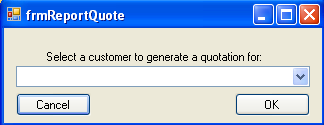
\includegraphics[scale=0.5]{frmReportQuote_scrot}
	\makeatletter
\def\PY@reset{\let\PY@it=\relax \let\PY@bf=\relax%
    \let\PY@ul=\relax \let\PY@tc=\relax%
    \let\PY@bc=\relax \let\PY@ff=\relax}
\def\PY@tok#1{\csname PY@tok@#1\endcsname}
\def\PY@toks#1+{\ifx\relax#1\empty\else%
    \PY@tok{#1}\expandafter\PY@toks\fi}
\def\PY@do#1{\PY@bc{\PY@tc{\PY@ul{%
    \PY@it{\PY@bf{\PY@ff{#1}}}}}}}
\def\PY#1#2{\PY@reset\PY@toks#1+\relax+\PY@do{#2}}

\expandafter\def\csname PY@tok@gd\endcsname{\def\PY@tc##1{\textcolor[rgb]{0.63,0.00,0.00}{##1}}}
\expandafter\def\csname PY@tok@gu\endcsname{\let\PY@bf=\textbf\def\PY@tc##1{\textcolor[rgb]{0.50,0.00,0.50}{##1}}}
\expandafter\def\csname PY@tok@gt\endcsname{\def\PY@tc##1{\textcolor[rgb]{0.00,0.25,0.82}{##1}}}
\expandafter\def\csname PY@tok@gs\endcsname{\let\PY@bf=\textbf}
\expandafter\def\csname PY@tok@gr\endcsname{\def\PY@tc##1{\textcolor[rgb]{1.00,0.00,0.00}{##1}}}
\expandafter\def\csname PY@tok@cm\endcsname{\let\PY@it=\textit\def\PY@tc##1{\textcolor[rgb]{0.25,0.50,0.50}{##1}}}
\expandafter\def\csname PY@tok@vg\endcsname{\def\PY@tc##1{\textcolor[rgb]{0.10,0.09,0.49}{##1}}}
\expandafter\def\csname PY@tok@m\endcsname{\def\PY@tc##1{\textcolor[rgb]{0.40,0.40,0.40}{##1}}}
\expandafter\def\csname PY@tok@mh\endcsname{\def\PY@tc##1{\textcolor[rgb]{0.40,0.40,0.40}{##1}}}
\expandafter\def\csname PY@tok@go\endcsname{\def\PY@tc##1{\textcolor[rgb]{0.50,0.50,0.50}{##1}}}
\expandafter\def\csname PY@tok@ge\endcsname{\let\PY@it=\textit}
\expandafter\def\csname PY@tok@vc\endcsname{\def\PY@tc##1{\textcolor[rgb]{0.10,0.09,0.49}{##1}}}
\expandafter\def\csname PY@tok@il\endcsname{\def\PY@tc##1{\textcolor[rgb]{0.40,0.40,0.40}{##1}}}
\expandafter\def\csname PY@tok@cs\endcsname{\let\PY@it=\textit\def\PY@tc##1{\textcolor[rgb]{0.25,0.50,0.50}{##1}}}
\expandafter\def\csname PY@tok@cp\endcsname{\def\PY@tc##1{\textcolor[rgb]{0.74,0.48,0.00}{##1}}}
\expandafter\def\csname PY@tok@gi\endcsname{\def\PY@tc##1{\textcolor[rgb]{0.00,0.63,0.00}{##1}}}
\expandafter\def\csname PY@tok@gh\endcsname{\let\PY@bf=\textbf\def\PY@tc##1{\textcolor[rgb]{0.00,0.00,0.50}{##1}}}
\expandafter\def\csname PY@tok@ni\endcsname{\let\PY@bf=\textbf\def\PY@tc##1{\textcolor[rgb]{0.60,0.60,0.60}{##1}}}
\expandafter\def\csname PY@tok@nl\endcsname{\def\PY@tc##1{\textcolor[rgb]{0.63,0.63,0.00}{##1}}}
\expandafter\def\csname PY@tok@nn\endcsname{\let\PY@bf=\textbf\def\PY@tc##1{\textcolor[rgb]{0.00,0.00,1.00}{##1}}}
\expandafter\def\csname PY@tok@no\endcsname{\def\PY@tc##1{\textcolor[rgb]{0.53,0.00,0.00}{##1}}}
\expandafter\def\csname PY@tok@na\endcsname{\def\PY@tc##1{\textcolor[rgb]{0.49,0.56,0.16}{##1}}}
\expandafter\def\csname PY@tok@nb\endcsname{\def\PY@tc##1{\textcolor[rgb]{0.00,0.50,0.00}{##1}}}
\expandafter\def\csname PY@tok@nc\endcsname{\let\PY@bf=\textbf\def\PY@tc##1{\textcolor[rgb]{0.00,0.00,1.00}{##1}}}
\expandafter\def\csname PY@tok@nd\endcsname{\def\PY@tc##1{\textcolor[rgb]{0.67,0.13,1.00}{##1}}}
\expandafter\def\csname PY@tok@ne\endcsname{\let\PY@bf=\textbf\def\PY@tc##1{\textcolor[rgb]{0.82,0.25,0.23}{##1}}}
\expandafter\def\csname PY@tok@nf\endcsname{\def\PY@tc##1{\textcolor[rgb]{0.00,0.00,1.00}{##1}}}
\expandafter\def\csname PY@tok@si\endcsname{\let\PY@bf=\textbf\def\PY@tc##1{\textcolor[rgb]{0.73,0.40,0.53}{##1}}}
\expandafter\def\csname PY@tok@s2\endcsname{\def\PY@tc##1{\textcolor[rgb]{0.73,0.13,0.13}{##1}}}
\expandafter\def\csname PY@tok@vi\endcsname{\def\PY@tc##1{\textcolor[rgb]{0.10,0.09,0.49}{##1}}}
\expandafter\def\csname PY@tok@nt\endcsname{\let\PY@bf=\textbf\def\PY@tc##1{\textcolor[rgb]{0.00,0.50,0.00}{##1}}}
\expandafter\def\csname PY@tok@nv\endcsname{\def\PY@tc##1{\textcolor[rgb]{0.10,0.09,0.49}{##1}}}
\expandafter\def\csname PY@tok@s1\endcsname{\def\PY@tc##1{\textcolor[rgb]{0.73,0.13,0.13}{##1}}}
\expandafter\def\csname PY@tok@sh\endcsname{\def\PY@tc##1{\textcolor[rgb]{0.73,0.13,0.13}{##1}}}
\expandafter\def\csname PY@tok@sc\endcsname{\def\PY@tc##1{\textcolor[rgb]{0.73,0.13,0.13}{##1}}}
\expandafter\def\csname PY@tok@sx\endcsname{\def\PY@tc##1{\textcolor[rgb]{0.00,0.50,0.00}{##1}}}
\expandafter\def\csname PY@tok@bp\endcsname{\def\PY@tc##1{\textcolor[rgb]{0.00,0.50,0.00}{##1}}}
\expandafter\def\csname PY@tok@c1\endcsname{\let\PY@it=\textit\def\PY@tc##1{\textcolor[rgb]{0.25,0.50,0.50}{##1}}}
\expandafter\def\csname PY@tok@kc\endcsname{\let\PY@bf=\textbf\def\PY@tc##1{\textcolor[rgb]{0.00,0.50,0.00}{##1}}}
\expandafter\def\csname PY@tok@c\endcsname{\let\PY@it=\textit\def\PY@tc##1{\textcolor[rgb]{0.25,0.50,0.50}{##1}}}
\expandafter\def\csname PY@tok@mf\endcsname{\def\PY@tc##1{\textcolor[rgb]{0.40,0.40,0.40}{##1}}}
\expandafter\def\csname PY@tok@err\endcsname{\def\PY@bc##1{\setlength{\fboxsep}{0pt}\fcolorbox[rgb]{1.00,0.00,0.00}{1,1,1}{\strut ##1}}}
\expandafter\def\csname PY@tok@kd\endcsname{\let\PY@bf=\textbf\def\PY@tc##1{\textcolor[rgb]{0.00,0.50,0.00}{##1}}}
\expandafter\def\csname PY@tok@ss\endcsname{\def\PY@tc##1{\textcolor[rgb]{0.10,0.09,0.49}{##1}}}
\expandafter\def\csname PY@tok@sr\endcsname{\def\PY@tc##1{\textcolor[rgb]{0.73,0.40,0.53}{##1}}}
\expandafter\def\csname PY@tok@mo\endcsname{\def\PY@tc##1{\textcolor[rgb]{0.40,0.40,0.40}{##1}}}
\expandafter\def\csname PY@tok@kn\endcsname{\let\PY@bf=\textbf\def\PY@tc##1{\textcolor[rgb]{0.00,0.50,0.00}{##1}}}
\expandafter\def\csname PY@tok@mi\endcsname{\def\PY@tc##1{\textcolor[rgb]{0.40,0.40,0.40}{##1}}}
\expandafter\def\csname PY@tok@gp\endcsname{\let\PY@bf=\textbf\def\PY@tc##1{\textcolor[rgb]{0.00,0.00,0.50}{##1}}}
\expandafter\def\csname PY@tok@o\endcsname{\def\PY@tc##1{\textcolor[rgb]{0.40,0.40,0.40}{##1}}}
\expandafter\def\csname PY@tok@kr\endcsname{\let\PY@bf=\textbf\def\PY@tc##1{\textcolor[rgb]{0.00,0.50,0.00}{##1}}}
\expandafter\def\csname PY@tok@s\endcsname{\def\PY@tc##1{\textcolor[rgb]{0.73,0.13,0.13}{##1}}}
\expandafter\def\csname PY@tok@kp\endcsname{\def\PY@tc##1{\textcolor[rgb]{0.00,0.50,0.00}{##1}}}
\expandafter\def\csname PY@tok@w\endcsname{\def\PY@tc##1{\textcolor[rgb]{0.73,0.73,0.73}{##1}}}
\expandafter\def\csname PY@tok@kt\endcsname{\def\PY@tc##1{\textcolor[rgb]{0.69,0.00,0.25}{##1}}}
\expandafter\def\csname PY@tok@ow\endcsname{\let\PY@bf=\textbf\def\PY@tc##1{\textcolor[rgb]{0.67,0.13,1.00}{##1}}}
\expandafter\def\csname PY@tok@sb\endcsname{\def\PY@tc##1{\textcolor[rgb]{0.73,0.13,0.13}{##1}}}
\expandafter\def\csname PY@tok@k\endcsname{\let\PY@bf=\textbf\def\PY@tc##1{\textcolor[rgb]{0.00,0.50,0.00}{##1}}}
\expandafter\def\csname PY@tok@se\endcsname{\let\PY@bf=\textbf\def\PY@tc##1{\textcolor[rgb]{0.73,0.40,0.13}{##1}}}
\expandafter\def\csname PY@tok@sd\endcsname{\let\PY@it=\textit\def\PY@tc##1{\textcolor[rgb]{0.73,0.13,0.13}{##1}}}

\def\PYZbs{\char`\\}
\def\PYZus{\char`\_}
\def\PYZob{\char`\{}
\def\PYZcb{\char`\}}
\def\PYZca{\char`\^}
\def\PYZam{\char`\&}
\def\PYZlt{\char`\<}
\def\PYZgt{\char`\>}
\def\PYZsh{\char`\#}
\def\PYZpc{\char`\%}
\def\PYZdl{\char`\$}
\def\PYZti{\char`\~}
% for compatibility with earlier versions
\def\PYZat{@}
\def\PYZlb{[}
\def\PYZrb{]}
\makeatother

\begin{Verbatim}[commandchars=\\\{\}]
\PY{k}{Imports} \PY{n+nn}{System.Data}
\PY{k}{Imports} \PY{n+nn}{System.Data.OleDb}

\PY{k}{Public} \PY{k}{Class} \PY{n+nc}{frmReportQuote}
    \PY{c}{'THIS CODE SATISFIES SPECIFIC OBJECTIVE 12.}
    \PY{k}{Public} \PY{n}{accConnection} \PY{o+ow}{As} \PY{k}{New} \PY{n}{OleDbConnection}

    \PY{k}{Private} \PY{k}{Sub} \PY{n+nf}{frmReportQuote\PYZus{}Load}\PY{p}{(}\PY{k}{ByVal} \PY{n}{sender} \PY{o+ow}{As} \PY{n}{System}\PY{p}{.}\PY{n}{Object}\PY{p}{,} \PY{n}{\PYZus{}}
                                    \PY{k}{ByVal} \PY{n}{e} \PY{o+ow}{As} \PY{n}{System}\PY{p}{.}\PY{n}{EventArgs}\PY{p}{)} \PY{k}{Handles} \PY{k}{MyBase}\PY{p}{.}\PY{n}{Load}

        \PY{k}{If} \PY{n}{frmLoginForm}\PY{p}{.}\PY{n}{accConnection}\PY{p}{.}\PY{n}{State} \PY{o}{\PYZlt{}\PYZgt{}} \PY{n}{ConnectionState}\PY{p}{.}\PY{n}{Open} \PY{k}{Then}
            \PY{n}{frmLoginForm}\PY{p}{.}\PY{n}{accConnection}\PY{p}{.}\PY{n}{Open}\PY{p}{(}\PY{p}{)}
        \PY{k}{End} \PY{k}{If}

        \PY{n}{accConnection} \PY{o}{=} \PY{n}{frmLoginForm}\PY{p}{.}\PY{n}{accConnection}
        \PY{k}{Dim} \PY{n}{strSQL} \PY{o+ow}{As} \PY{k+kt}{String} \PY{o}{=} \PY{l+s}{"}\PY{l+s}{SELECT cust\PYZus{}name FROM Customer}\PY{l+s}{"}
        \PY{k}{Dim} \PY{n}{da} \PY{o+ow}{As} \PY{k}{New} \PY{n}{OleDbDataAdapter}\PY{p}{(}\PY{n}{strSQL}\PY{p}{,} \PY{n}{accConnection}\PY{p}{)}
        \PY{k}{Dim} \PY{n}{ds} \PY{o+ow}{As} \PY{k}{New} \PY{n}{DataSet}

        \PY{n}{da}\PY{p}{.}\PY{n}{Fill}\PY{p}{(}\PY{n}{ds}\PY{p}{,} \PY{l+s}{"}\PY{l+s}{Customer}\PY{l+s}{"}\PY{p}{)}

        \PY{k}{Dim} \PY{n}{dt} \PY{o+ow}{As} \PY{n}{DataTable} \PY{o}{=} \PY{n}{ds}\PY{p}{.}\PY{n}{Tables}\PY{p}{(}\PY{l+m+mi}{0}\PY{p}{)}
        \PY{k}{Dim} \PY{n}{dr} \PY{o+ow}{As} \PY{n}{DataRow}

        \PY{k}{For} \PY{k}{Each} \PY{n}{dr} \PY{o+ow}{In} \PY{n}{dt}\PY{p}{.}\PY{n}{Rows}\PY{p}{(}\PY{p}{)}
            \PY{c}{'List customer names in the box so that the user can select}
            \PY{c}{'a customer to show the quotation of.  At least customer details}
            \PY{c}{'will be inserted into the Word document at this stage.}
            \PY{n}{txtcbCustNameForQuotation}\PY{p}{.}\PY{n}{Items}\PY{p}{.}\PY{n}{Add}\PY{p}{(}\PY{n}{dr}\PY{p}{(}\PY{l+s}{"}\PY{l+s}{cust\PYZus{}name}\PY{l+s}{"}\PY{p}{)}\PY{p}{)}
        \PY{k}{Next}

        \PY{n}{txtcbCustNameForQuotation}\PY{p}{.}\PY{n}{SelectedIndex} \PY{o}{=} \PY{o}{-}\PY{l+m+mi}{1}

    \PY{k}{End} \PY{k}{Sub}

    \PY{k}{Private} \PY{k}{Sub} \PY{n+nf}{btnCancel\PYZus{}Click}\PY{p}{(}\PY{k}{ByVal} \PY{n}{sender} \PY{o+ow}{As} \PY{n}{System}\PY{p}{.}\PY{n}{Object}\PY{p}{,} \PY{n}{\PYZus{}}
                                \PY{k}{ByVal} \PY{n}{e} \PY{o+ow}{As} \PY{n}{System}\PY{p}{.}\PY{n}{EventArgs}\PY{p}{)} \PY{k}{Handles} \PY{n}{btnCancel}\PY{p}{.}\PY{n}{Click}
        \PY{k}{Me}\PY{p}{.}\PY{n}{Close}\PY{p}{(}\PY{p}{)}
        \PY{n}{frmReportMenu}\PY{p}{.}\PY{n}{Show}\PY{p}{(}\PY{p}{)}
    \PY{k}{End} \PY{k}{Sub}

    \PY{k}{Private} \PY{k}{Sub} \PY{n+nf}{btnOK2\PYZus{}Click}\PY{p}{(}\PY{k}{ByVal} \PY{n}{sender} \PY{o+ow}{As} \PY{n}{System}\PY{p}{.}\PY{n}{Object}\PY{p}{,} \PY{n}{\PYZus{}}
                             \PY{k}{ByVal} \PY{n}{e} \PY{o+ow}{As} \PY{n}{System}\PY{p}{.}\PY{n}{EventArgs}\PY{p}{)} \PY{k}{Handles} \PY{n}{btnOK2}\PY{p}{.}\PY{n}{Click}

        \PY{n}{accConnection} \PY{o}{=} \PY{n}{frmLoginForm}\PY{p}{.}\PY{n}{accConnection}
        \PY{c}{'Input customer name from the other form and attribute it to CTN.}
        \PY{k}{Dim} \PY{n}{ctn} \PY{o+ow}{As} \PY{k+kt}{String} \PY{o}{=} \PY{n}{txtcbCustNameForQuotation}\PY{p}{.}\PY{n}{SelectedItem}
        \PY{k}{Dim} \PY{n}{cmdString} \PY{o+ow}{As} \PY{k+kt}{String} \PY{o}{=} \PY{l+s}{"}\PY{l+s}{SELECT * FROM Customer WHERE cust\PYZus{}name = '}\PY{l+s}{"} \PY{o}{\PYZam{}} \PY{n}{ctn} \PY{o}{\PYZam{}} \PY{l+s}{"}\PY{l+s}{'}\PY{l+s}{"}

        \PY{k}{Dim} \PY{n}{accCommand} \PY{o+ow}{As} \PY{k}{New} \PY{n}{OleDbCommand}
        \PY{k}{Dim} \PY{n}{da} \PY{o+ow}{As} \PY{k}{New} \PY{n}{OleDbDataAdapter}\PY{p}{(}\PY{n}{cmdString}\PY{p}{,} \PY{n}{accConnection}\PY{p}{)}
        \PY{k}{Dim} \PY{n}{ds} \PY{o+ow}{As} \PY{k}{New} \PY{n}{DataSet}

        \PY{n}{da}\PY{p}{.}\PY{n}{Fill}\PY{p}{(}\PY{n}{ds}\PY{p}{,} \PY{l+s}{"}\PY{l+s}{Customer}\PY{l+s}{"}\PY{p}{)}

        \PY{k}{Dim} \PY{n}{dt} \PY{o+ow}{As} \PY{n}{DataTable} \PY{o}{=} \PY{n}{ds}\PY{p}{.}\PY{n}{Tables}\PY{p}{(}\PY{l+m+mi}{0}\PY{p}{)}

        \PY{c}{'Now create variables to hold the useful address values of the}
        \PY{c}{''* FROM Customer' so they'll be useful later on for the Word}
        \PY{c}{'quotation stuff.}
        \PY{c}{'aqcn, for example, = add quotation cust name}
        \PY{k}{Dim} \PY{n}{aqct} \PY{o+ow}{As} \PY{k+kt}{String} \PY{o}{=} \PY{n}{ds}\PY{p}{.}\PY{n}{Tables}\PY{p}{(}\PY{l+m+mi}{0}\PY{p}{)}\PY{p}{.}\PY{n}{Rows}\PY{p}{(}\PY{l+m+mi}{0}\PY{p}{)}\PY{p}{.}\PY{n}{Item}\PY{p}{(}\PY{l+s}{"}\PY{l+s}{cust\PYZus{}title}\PY{l+s}{"}\PY{p}{)}
        \PY{k}{Dim} \PY{n}{aqcn} \PY{o+ow}{As} \PY{k+kt}{String} \PY{o}{=} \PY{n}{ds}\PY{p}{.}\PY{n}{Tables}\PY{p}{(}\PY{l+m+mi}{0}\PY{p}{)}\PY{p}{.}\PY{n}{Rows}\PY{p}{(}\PY{l+m+mi}{0}\PY{p}{)}\PY{p}{.}\PY{n}{Item}\PY{p}{(}\PY{l+s}{"}\PY{l+s}{cust\PYZus{}name}\PY{l+s}{"}\PY{p}{)}
        \PY{c}{'Billing address and postcode in this case.}
        \PY{k}{Dim} \PY{n}{aqca} \PY{o+ow}{As} \PY{k+kt}{String} \PY{o}{=} \PY{n}{ds}\PY{p}{.}\PY{n}{Tables}\PY{p}{(}\PY{l+m+mi}{0}\PY{p}{)}\PY{p}{.}\PY{n}{Rows}\PY{p}{(}\PY{l+m+mi}{0}\PY{p}{)}\PY{p}{.}\PY{n}{Item}\PY{p}{(}\PY{l+s}{"}\PY{l+s}{cust\PYZus{}billaddress}\PY{l+s}{"}\PY{p}{)}
        \PY{k}{Dim} \PY{n}{aqcp} \PY{o+ow}{As} \PY{k+kt}{String} \PY{o}{=} \PY{n}{ds}\PY{p}{.}\PY{n}{Tables}\PY{p}{(}\PY{l+m+mi}{0}\PY{p}{)}\PY{p}{.}\PY{n}{Rows}\PY{p}{(}\PY{l+m+mi}{0}\PY{p}{)}\PY{p}{.}\PY{n}{Item}\PY{p}{(}\PY{l+s}{"}\PY{l+s}{cust\PYZus{}billpostcode}\PY{l+s}{"}\PY{p}{)}

        \PY{c}{'Now for some Word automation magic.  Call a procedure to do this}
        \PY{c}{'to save cluttering this OK button's execution with code.}
        \PY{k}{Call} \PY{n}{frmSwankyCode}\PY{p}{.}\PY{n}{WordQuotationAutomationMagic}\PY{p}{(}\PY{n}{aqct}\PY{p}{,} \PY{n}{aqcn}\PY{p}{,} \PY{n}{aqca}\PY{p}{,} \PY{n}{aqcp}\PY{p}{)}

    \PY{k}{End} \PY{k}{Sub}
\PY{k}{End} \PY{k}{Class}
\end{Verbatim}

\subsection{frmReportLog}
	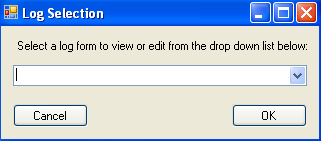
\includegraphics[scale=0.5]{frmReportLog_scrot}
	\makeatletter
\def\PY@reset{\let\PY@it=\relax \let\PY@bf=\relax%
    \let\PY@ul=\relax \let\PY@tc=\relax%
    \let\PY@bc=\relax \let\PY@ff=\relax}
\def\PY@tok#1{\csname PY@tok@#1\endcsname}
\def\PY@toks#1+{\ifx\relax#1\empty\else%
    \PY@tok{#1}\expandafter\PY@toks\fi}
\def\PY@do#1{\PY@bc{\PY@tc{\PY@ul{%
    \PY@it{\PY@bf{\PY@ff{#1}}}}}}}
\def\PY#1#2{\PY@reset\PY@toks#1+\relax+\PY@do{#2}}

\expandafter\def\csname PY@tok@gd\endcsname{\def\PY@tc##1{\textcolor[rgb]{0.63,0.00,0.00}{##1}}}
\expandafter\def\csname PY@tok@gu\endcsname{\let\PY@bf=\textbf\def\PY@tc##1{\textcolor[rgb]{0.50,0.00,0.50}{##1}}}
\expandafter\def\csname PY@tok@gt\endcsname{\def\PY@tc##1{\textcolor[rgb]{0.00,0.25,0.82}{##1}}}
\expandafter\def\csname PY@tok@gs\endcsname{\let\PY@bf=\textbf}
\expandafter\def\csname PY@tok@gr\endcsname{\def\PY@tc##1{\textcolor[rgb]{1.00,0.00,0.00}{##1}}}
\expandafter\def\csname PY@tok@cm\endcsname{\let\PY@it=\textit\def\PY@tc##1{\textcolor[rgb]{0.25,0.50,0.50}{##1}}}
\expandafter\def\csname PY@tok@vg\endcsname{\def\PY@tc##1{\textcolor[rgb]{0.10,0.09,0.49}{##1}}}
\expandafter\def\csname PY@tok@m\endcsname{\def\PY@tc##1{\textcolor[rgb]{0.40,0.40,0.40}{##1}}}
\expandafter\def\csname PY@tok@mh\endcsname{\def\PY@tc##1{\textcolor[rgb]{0.40,0.40,0.40}{##1}}}
\expandafter\def\csname PY@tok@go\endcsname{\def\PY@tc##1{\textcolor[rgb]{0.50,0.50,0.50}{##1}}}
\expandafter\def\csname PY@tok@ge\endcsname{\let\PY@it=\textit}
\expandafter\def\csname PY@tok@vc\endcsname{\def\PY@tc##1{\textcolor[rgb]{0.10,0.09,0.49}{##1}}}
\expandafter\def\csname PY@tok@il\endcsname{\def\PY@tc##1{\textcolor[rgb]{0.40,0.40,0.40}{##1}}}
\expandafter\def\csname PY@tok@cs\endcsname{\let\PY@it=\textit\def\PY@tc##1{\textcolor[rgb]{0.25,0.50,0.50}{##1}}}
\expandafter\def\csname PY@tok@cp\endcsname{\def\PY@tc##1{\textcolor[rgb]{0.74,0.48,0.00}{##1}}}
\expandafter\def\csname PY@tok@gi\endcsname{\def\PY@tc##1{\textcolor[rgb]{0.00,0.63,0.00}{##1}}}
\expandafter\def\csname PY@tok@gh\endcsname{\let\PY@bf=\textbf\def\PY@tc##1{\textcolor[rgb]{0.00,0.00,0.50}{##1}}}
\expandafter\def\csname PY@tok@ni\endcsname{\let\PY@bf=\textbf\def\PY@tc##1{\textcolor[rgb]{0.60,0.60,0.60}{##1}}}
\expandafter\def\csname PY@tok@nl\endcsname{\def\PY@tc##1{\textcolor[rgb]{0.63,0.63,0.00}{##1}}}
\expandafter\def\csname PY@tok@nn\endcsname{\let\PY@bf=\textbf\def\PY@tc##1{\textcolor[rgb]{0.00,0.00,1.00}{##1}}}
\expandafter\def\csname PY@tok@no\endcsname{\def\PY@tc##1{\textcolor[rgb]{0.53,0.00,0.00}{##1}}}
\expandafter\def\csname PY@tok@na\endcsname{\def\PY@tc##1{\textcolor[rgb]{0.49,0.56,0.16}{##1}}}
\expandafter\def\csname PY@tok@nb\endcsname{\def\PY@tc##1{\textcolor[rgb]{0.00,0.50,0.00}{##1}}}
\expandafter\def\csname PY@tok@nc\endcsname{\let\PY@bf=\textbf\def\PY@tc##1{\textcolor[rgb]{0.00,0.00,1.00}{##1}}}
\expandafter\def\csname PY@tok@nd\endcsname{\def\PY@tc##1{\textcolor[rgb]{0.67,0.13,1.00}{##1}}}
\expandafter\def\csname PY@tok@ne\endcsname{\let\PY@bf=\textbf\def\PY@tc##1{\textcolor[rgb]{0.82,0.25,0.23}{##1}}}
\expandafter\def\csname PY@tok@nf\endcsname{\def\PY@tc##1{\textcolor[rgb]{0.00,0.00,1.00}{##1}}}
\expandafter\def\csname PY@tok@si\endcsname{\let\PY@bf=\textbf\def\PY@tc##1{\textcolor[rgb]{0.73,0.40,0.53}{##1}}}
\expandafter\def\csname PY@tok@s2\endcsname{\def\PY@tc##1{\textcolor[rgb]{0.73,0.13,0.13}{##1}}}
\expandafter\def\csname PY@tok@vi\endcsname{\def\PY@tc##1{\textcolor[rgb]{0.10,0.09,0.49}{##1}}}
\expandafter\def\csname PY@tok@nt\endcsname{\let\PY@bf=\textbf\def\PY@tc##1{\textcolor[rgb]{0.00,0.50,0.00}{##1}}}
\expandafter\def\csname PY@tok@nv\endcsname{\def\PY@tc##1{\textcolor[rgb]{0.10,0.09,0.49}{##1}}}
\expandafter\def\csname PY@tok@s1\endcsname{\def\PY@tc##1{\textcolor[rgb]{0.73,0.13,0.13}{##1}}}
\expandafter\def\csname PY@tok@sh\endcsname{\def\PY@tc##1{\textcolor[rgb]{0.73,0.13,0.13}{##1}}}
\expandafter\def\csname PY@tok@sc\endcsname{\def\PY@tc##1{\textcolor[rgb]{0.73,0.13,0.13}{##1}}}
\expandafter\def\csname PY@tok@sx\endcsname{\def\PY@tc##1{\textcolor[rgb]{0.00,0.50,0.00}{##1}}}
\expandafter\def\csname PY@tok@bp\endcsname{\def\PY@tc##1{\textcolor[rgb]{0.00,0.50,0.00}{##1}}}
\expandafter\def\csname PY@tok@c1\endcsname{\let\PY@it=\textit\def\PY@tc##1{\textcolor[rgb]{0.25,0.50,0.50}{##1}}}
\expandafter\def\csname PY@tok@kc\endcsname{\let\PY@bf=\textbf\def\PY@tc##1{\textcolor[rgb]{0.00,0.50,0.00}{##1}}}
\expandafter\def\csname PY@tok@c\endcsname{\let\PY@it=\textit\def\PY@tc##1{\textcolor[rgb]{0.25,0.50,0.50}{##1}}}
\expandafter\def\csname PY@tok@mf\endcsname{\def\PY@tc##1{\textcolor[rgb]{0.40,0.40,0.40}{##1}}}
\expandafter\def\csname PY@tok@err\endcsname{\def\PY@bc##1{\setlength{\fboxsep}{0pt}\fcolorbox[rgb]{1.00,0.00,0.00}{1,1,1}{\strut ##1}}}
\expandafter\def\csname PY@tok@kd\endcsname{\let\PY@bf=\textbf\def\PY@tc##1{\textcolor[rgb]{0.00,0.50,0.00}{##1}}}
\expandafter\def\csname PY@tok@ss\endcsname{\def\PY@tc##1{\textcolor[rgb]{0.10,0.09,0.49}{##1}}}
\expandafter\def\csname PY@tok@sr\endcsname{\def\PY@tc##1{\textcolor[rgb]{0.73,0.40,0.53}{##1}}}
\expandafter\def\csname PY@tok@mo\endcsname{\def\PY@tc##1{\textcolor[rgb]{0.40,0.40,0.40}{##1}}}
\expandafter\def\csname PY@tok@kn\endcsname{\let\PY@bf=\textbf\def\PY@tc##1{\textcolor[rgb]{0.00,0.50,0.00}{##1}}}
\expandafter\def\csname PY@tok@mi\endcsname{\def\PY@tc##1{\textcolor[rgb]{0.40,0.40,0.40}{##1}}}
\expandafter\def\csname PY@tok@gp\endcsname{\let\PY@bf=\textbf\def\PY@tc##1{\textcolor[rgb]{0.00,0.00,0.50}{##1}}}
\expandafter\def\csname PY@tok@o\endcsname{\def\PY@tc##1{\textcolor[rgb]{0.40,0.40,0.40}{##1}}}
\expandafter\def\csname PY@tok@kr\endcsname{\let\PY@bf=\textbf\def\PY@tc##1{\textcolor[rgb]{0.00,0.50,0.00}{##1}}}
\expandafter\def\csname PY@tok@s\endcsname{\def\PY@tc##1{\textcolor[rgb]{0.73,0.13,0.13}{##1}}}
\expandafter\def\csname PY@tok@kp\endcsname{\def\PY@tc##1{\textcolor[rgb]{0.00,0.50,0.00}{##1}}}
\expandafter\def\csname PY@tok@w\endcsname{\def\PY@tc##1{\textcolor[rgb]{0.73,0.73,0.73}{##1}}}
\expandafter\def\csname PY@tok@kt\endcsname{\def\PY@tc##1{\textcolor[rgb]{0.69,0.00,0.25}{##1}}}
\expandafter\def\csname PY@tok@ow\endcsname{\let\PY@bf=\textbf\def\PY@tc##1{\textcolor[rgb]{0.67,0.13,1.00}{##1}}}
\expandafter\def\csname PY@tok@sb\endcsname{\def\PY@tc##1{\textcolor[rgb]{0.73,0.13,0.13}{##1}}}
\expandafter\def\csname PY@tok@k\endcsname{\let\PY@bf=\textbf\def\PY@tc##1{\textcolor[rgb]{0.00,0.50,0.00}{##1}}}
\expandafter\def\csname PY@tok@se\endcsname{\let\PY@bf=\textbf\def\PY@tc##1{\textcolor[rgb]{0.73,0.40,0.13}{##1}}}
\expandafter\def\csname PY@tok@sd\endcsname{\let\PY@it=\textit\def\PY@tc##1{\textcolor[rgb]{0.73,0.13,0.13}{##1}}}

\def\PYZbs{\char`\\}
\def\PYZus{\char`\_}
\def\PYZob{\char`\{}
\def\PYZcb{\char`\}}
\def\PYZca{\char`\^}
\def\PYZam{\char`\&}
\def\PYZlt{\char`\<}
\def\PYZgt{\char`\>}
\def\PYZsh{\char`\#}
\def\PYZpc{\char`\%}
\def\PYZdl{\char`\$}
\def\PYZti{\char`\~}
% for compatibility with earlier versions
\def\PYZat{@}
\def\PYZlb{[}
\def\PYZrb{]}
\makeatother

\begin{Verbatim}[commandchars=\\\{\}]
\PY{err}{�}\PY{err}{�}\PY{err}{�}\PY{k}{Imports} \PY{n+nn}{Microsoft.Office.Core}
\PY{k}{Imports} \PY{n+nn}{Microsoft.Office.Interop}
\PY{k}{Imports} \PY{n+nn}{Microsoft.Office.Interop.Word}

\PY{k}{Public} \PY{k}{Class} \PY{n+nc}{frmReportLog}
    \PY{c}{'THIS CODE SATISFIES SPECIFIC OBJECTIVE 12.}

    \PY{k}{Private} \PY{k}{Sub} \PY{n+nf}{frmReportLog\PYZus{}Load}\PY{p}{(}\PY{k}{ByVal} \PY{n}{sender} \PY{o+ow}{As} \PY{n}{System}\PY{p}{.}\PY{n}{Object}\PY{p}{,} \PY{n}{\PYZus{}}
                                  \PY{k}{ByVal} \PY{n}{e} \PY{o+ow}{As} \PY{n}{System}\PY{p}{.}\PY{n}{EventArgs}\PY{p}{)} \PY{k}{Handles} \PY{k}{MyBase}\PY{p}{.}\PY{n}{Load}

        \PY{c}{'Drop down menu populated with months up to 12/12.}
        \PY{n}{txtcbReportLog}\PY{p}{.}\PY{n}{Items}\PY{p}{.}\PY{n}{Add}\PY{p}{(}\PY{l+s}{"}\PY{l+s}{December 2011}\PY{l+s}{"}\PY{p}{)}
        \PY{n}{txtcbReportLog}\PY{p}{.}\PY{n}{Items}\PY{p}{.}\PY{n}{Add}\PY{p}{(}\PY{l+s}{"}\PY{l+s}{January 2012}\PY{l+s}{"}\PY{p}{)}
        \PY{n}{txtcbReportLog}\PY{p}{.}\PY{n}{Items}\PY{p}{.}\PY{n}{Add}\PY{p}{(}\PY{l+s}{"}\PY{l+s}{February 2012}\PY{l+s}{"}\PY{p}{)}
        \PY{n}{txtcbReportLog}\PY{p}{.}\PY{n}{Items}\PY{p}{.}\PY{n}{Add}\PY{p}{(}\PY{l+s}{"}\PY{l+s}{March 2012}\PY{l+s}{"}\PY{p}{)}
        \PY{n}{txtcbReportLog}\PY{p}{.}\PY{n}{Items}\PY{p}{.}\PY{n}{Add}\PY{p}{(}\PY{l+s}{"}\PY{l+s}{April 2012}\PY{l+s}{"}\PY{p}{)}
        \PY{n}{txtcbReportLog}\PY{p}{.}\PY{n}{Items}\PY{p}{.}\PY{n}{Add}\PY{p}{(}\PY{l+s}{"}\PY{l+s}{May 2012}\PY{l+s}{"}\PY{p}{)}
        \PY{n}{txtcbReportLog}\PY{p}{.}\PY{n}{Items}\PY{p}{.}\PY{n}{Add}\PY{p}{(}\PY{l+s}{"}\PY{l+s}{June 2012}\PY{l+s}{"}\PY{p}{)}
        \PY{n}{txtcbReportLog}\PY{p}{.}\PY{n}{Items}\PY{p}{.}\PY{n}{Add}\PY{p}{(}\PY{l+s}{"}\PY{l+s}{July 2012}\PY{l+s}{"}\PY{p}{)}
        \PY{n}{txtcbReportLog}\PY{p}{.}\PY{n}{Items}\PY{p}{.}\PY{n}{Add}\PY{p}{(}\PY{l+s}{"}\PY{l+s}{August 2012}\PY{l+s}{"}\PY{p}{)}
        \PY{n}{txtcbReportLog}\PY{p}{.}\PY{n}{Items}\PY{p}{.}\PY{n}{Add}\PY{p}{(}\PY{l+s}{"}\PY{l+s}{September 2012}\PY{l+s}{"}\PY{p}{)}
        \PY{n}{txtcbReportLog}\PY{p}{.}\PY{n}{Items}\PY{p}{.}\PY{n}{Add}\PY{p}{(}\PY{l+s}{"}\PY{l+s}{October 2012}\PY{l+s}{"}\PY{p}{)}
        \PY{n}{txtcbReportLog}\PY{p}{.}\PY{n}{Items}\PY{p}{.}\PY{n}{Add}\PY{p}{(}\PY{l+s}{"}\PY{l+s}{November 2012}\PY{l+s}{"}\PY{p}{)}
        \PY{n}{txtcbReportLog}\PY{p}{.}\PY{n}{Items}\PY{p}{.}\PY{n}{Add}\PY{p}{(}\PY{l+s}{"}\PY{l+s}{December 2012}\PY{l+s}{"}\PY{p}{)}

    \PY{k}{End} \PY{k}{Sub}

    \PY{k}{Private} \PY{k}{Sub} \PY{n+nf}{btnOK\PYZus{}Click}\PY{p}{(}\PY{k}{ByVal} \PY{n}{sender} \PY{o+ow}{As} \PY{n}{System}\PY{p}{.}\PY{n}{Object}\PY{p}{,} \PY{n}{\PYZus{}}
                            \PY{k}{ByVal} \PY{n}{e} \PY{o+ow}{As} \PY{n}{System}\PY{p}{.}\PY{n}{EventArgs}\PY{p}{)} \PY{k}{Handles} \PY{n}{btnOK}\PY{p}{.}\PY{n}{Click}
        \PY{c}{'On click, open the selected file from the drop down list with}
        \PY{c}{'Microsoft Word.}

        \PY{k}{Dim} \PY{n}{ms\PYZus{}word} \PY{o+ow}{As} \PY{k}{New} \PY{n}{Word}\PY{p}{.}\PY{n}{Application}
        \PY{k}{Dim} \PY{n}{worddoc} \PY{o+ow}{As} \PY{k}{New} \PY{n}{Word}\PY{p}{.}\PY{n}{Document}

        \PY{c}{'Make the name shorter purely for ease of typing, despite Visual}
        \PY{c}{'Studio's tab completion.}
        \PY{k}{Dim} \PY{n}{rlsi} \PY{o+ow}{As} \PY{k+kt}{String} \PY{o}{=} \PY{n}{txtcbReportLog}\PY{p}{.}\PY{n}{SelectedItem}

        \PY{c}{'Now open the correct log form.}
        \PY{c}{'Get the left and right characters of the string 'rlsi'.}
        \PY{c}{'Make a new string out of those (in the format}
        \PY{c}{'E:\PYZbs{}sfsstuff\PYZbs{}log\PYZus{}[beginninglettersofmonth][enddigitsofyear].docx)}
        \PY{c}{'and put it directly into the doc opening, i.e. log\PYZus{}dec11.docx.}
		\PY{c}{'Make the filename all lowercase.}
        \PY{k}{Dim} \PY{n}{filename} \PY{o+ow}{As} \PY{k+kt}{String} \PY{o}{=} \PY{n}{Strings}\PY{p}{.}\PY{n}{Left}\PY{p}{(}\PY{n}{rlsi}\PY{p}{,} \PY{l+m+mi}{3}\PY{p}{)} \PY{o}{+} \PY{n}{Strings}\PY{p}{.}\PY{n}{Right}\PY{p}{(}\PY{n}{rlsi}\PY{p}{,} \PY{l+m+mi}{2}\PY{p}{)}
        \PY{n}{ms\PYZus{}word}\PY{p}{.}\PY{n}{Documents}\PY{p}{.}\PY{n}{Open}\PY{p}{(}\PY{l+s}{"}\PY{l+s}{E:\PYZbs{}sfsstuff\PYZbs{}log\PYZus{}}\PY{l+s}{"} \PY{o}{+} \PY{n}{Strings}\PY{p}{.}\PY{n}{LCase}\PY{p}{(}\PY{n}{filename}\PY{p}{)} \PY{o}{+} \PY{l+s}{"}\PY{l+s}{.docx}\PY{l+s}{"}\PY{p}{)}

        \PY{c}{'Let the user see the document when it opens.}
        \PY{n}{ms\PYZus{}word}\PY{p}{.}\PY{n}{WindowState} \PY{o}{=} \PY{n}{Word}\PY{p}{.}\PY{n}{WdWindowState}\PY{p}{.}\PY{n}{wdWindowStateNormal}
        \PY{n}{ms\PYZus{}word}\PY{p}{.}\PY{n}{Visible} \PY{o}{=} \PY{k}{True}

    \PY{k}{End} \PY{k}{Sub}

    \PY{k}{Private} \PY{k}{Sub} \PY{n+nf}{btnCancel\PYZus{}Click}\PY{p}{(}\PY{k}{ByVal} \PY{n}{sender} \PY{o+ow}{As} \PY{n}{System}\PY{p}{.}\PY{n}{Object}\PY{p}{,} \PY{n}{\PYZus{}}
                                \PY{k}{ByVal} \PY{n}{e} \PY{o+ow}{As} \PY{n}{System}\PY{p}{.}\PY{n}{EventArgs}\PY{p}{)} \PY{k}{Handles} \PY{n}{btnCancel}\PY{p}{.}\PY{n}{Click}
        \PY{k}{Me}\PY{p}{.}\PY{n}{Close}\PY{p}{(}\PY{p}{)}
        \PY{n}{frmReportMenu}\PY{p}{.}\PY{n}{Show}\PY{p}{(}\PY{p}{)}
    \PY{k}{End} \PY{k}{Sub}
\PY{k}{End} \PY{k}{Class}
\end{Verbatim}
	
\subsection{frmReportSurvey}
	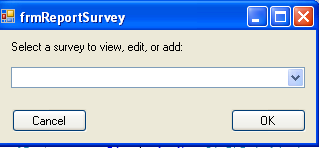
\includegraphics[scale=0.5]{frmReportSurvey_scrot}
	\makeatletter
\def\PY@reset{\let\PY@it=\relax \let\PY@bf=\relax%
    \let\PY@ul=\relax \let\PY@tc=\relax%
    \let\PY@bc=\relax \let\PY@ff=\relax}
\def\PY@tok#1{\csname PY@tok@#1\endcsname}
\def\PY@toks#1+{\ifx\relax#1\empty\else%
    \PY@tok{#1}\expandafter\PY@toks\fi}
\def\PY@do#1{\PY@bc{\PY@tc{\PY@ul{%
    \PY@it{\PY@bf{\PY@ff{#1}}}}}}}
\def\PY#1#2{\PY@reset\PY@toks#1+\relax+\PY@do{#2}}

\expandafter\def\csname PY@tok@gd\endcsname{\def\PY@tc##1{\textcolor[rgb]{0.63,0.00,0.00}{##1}}}
\expandafter\def\csname PY@tok@gu\endcsname{\let\PY@bf=\textbf\def\PY@tc##1{\textcolor[rgb]{0.50,0.00,0.50}{##1}}}
\expandafter\def\csname PY@tok@gt\endcsname{\def\PY@tc##1{\textcolor[rgb]{0.00,0.25,0.82}{##1}}}
\expandafter\def\csname PY@tok@gs\endcsname{\let\PY@bf=\textbf}
\expandafter\def\csname PY@tok@gr\endcsname{\def\PY@tc##1{\textcolor[rgb]{1.00,0.00,0.00}{##1}}}
\expandafter\def\csname PY@tok@cm\endcsname{\let\PY@it=\textit\def\PY@tc##1{\textcolor[rgb]{0.25,0.50,0.50}{##1}}}
\expandafter\def\csname PY@tok@vg\endcsname{\def\PY@tc##1{\textcolor[rgb]{0.10,0.09,0.49}{##1}}}
\expandafter\def\csname PY@tok@m\endcsname{\def\PY@tc##1{\textcolor[rgb]{0.40,0.40,0.40}{##1}}}
\expandafter\def\csname PY@tok@mh\endcsname{\def\PY@tc##1{\textcolor[rgb]{0.40,0.40,0.40}{##1}}}
\expandafter\def\csname PY@tok@go\endcsname{\def\PY@tc##1{\textcolor[rgb]{0.50,0.50,0.50}{##1}}}
\expandafter\def\csname PY@tok@ge\endcsname{\let\PY@it=\textit}
\expandafter\def\csname PY@tok@vc\endcsname{\def\PY@tc##1{\textcolor[rgb]{0.10,0.09,0.49}{##1}}}
\expandafter\def\csname PY@tok@il\endcsname{\def\PY@tc##1{\textcolor[rgb]{0.40,0.40,0.40}{##1}}}
\expandafter\def\csname PY@tok@cs\endcsname{\let\PY@it=\textit\def\PY@tc##1{\textcolor[rgb]{0.25,0.50,0.50}{##1}}}
\expandafter\def\csname PY@tok@cp\endcsname{\def\PY@tc##1{\textcolor[rgb]{0.74,0.48,0.00}{##1}}}
\expandafter\def\csname PY@tok@gi\endcsname{\def\PY@tc##1{\textcolor[rgb]{0.00,0.63,0.00}{##1}}}
\expandafter\def\csname PY@tok@gh\endcsname{\let\PY@bf=\textbf\def\PY@tc##1{\textcolor[rgb]{0.00,0.00,0.50}{##1}}}
\expandafter\def\csname PY@tok@ni\endcsname{\let\PY@bf=\textbf\def\PY@tc##1{\textcolor[rgb]{0.60,0.60,0.60}{##1}}}
\expandafter\def\csname PY@tok@nl\endcsname{\def\PY@tc##1{\textcolor[rgb]{0.63,0.63,0.00}{##1}}}
\expandafter\def\csname PY@tok@nn\endcsname{\let\PY@bf=\textbf\def\PY@tc##1{\textcolor[rgb]{0.00,0.00,1.00}{##1}}}
\expandafter\def\csname PY@tok@no\endcsname{\def\PY@tc##1{\textcolor[rgb]{0.53,0.00,0.00}{##1}}}
\expandafter\def\csname PY@tok@na\endcsname{\def\PY@tc##1{\textcolor[rgb]{0.49,0.56,0.16}{##1}}}
\expandafter\def\csname PY@tok@nb\endcsname{\def\PY@tc##1{\textcolor[rgb]{0.00,0.50,0.00}{##1}}}
\expandafter\def\csname PY@tok@nc\endcsname{\let\PY@bf=\textbf\def\PY@tc##1{\textcolor[rgb]{0.00,0.00,1.00}{##1}}}
\expandafter\def\csname PY@tok@nd\endcsname{\def\PY@tc##1{\textcolor[rgb]{0.67,0.13,1.00}{##1}}}
\expandafter\def\csname PY@tok@ne\endcsname{\let\PY@bf=\textbf\def\PY@tc##1{\textcolor[rgb]{0.82,0.25,0.23}{##1}}}
\expandafter\def\csname PY@tok@nf\endcsname{\def\PY@tc##1{\textcolor[rgb]{0.00,0.00,1.00}{##1}}}
\expandafter\def\csname PY@tok@si\endcsname{\let\PY@bf=\textbf\def\PY@tc##1{\textcolor[rgb]{0.73,0.40,0.53}{##1}}}
\expandafter\def\csname PY@tok@s2\endcsname{\def\PY@tc##1{\textcolor[rgb]{0.73,0.13,0.13}{##1}}}
\expandafter\def\csname PY@tok@vi\endcsname{\def\PY@tc##1{\textcolor[rgb]{0.10,0.09,0.49}{##1}}}
\expandafter\def\csname PY@tok@nt\endcsname{\let\PY@bf=\textbf\def\PY@tc##1{\textcolor[rgb]{0.00,0.50,0.00}{##1}}}
\expandafter\def\csname PY@tok@nv\endcsname{\def\PY@tc##1{\textcolor[rgb]{0.10,0.09,0.49}{##1}}}
\expandafter\def\csname PY@tok@s1\endcsname{\def\PY@tc##1{\textcolor[rgb]{0.73,0.13,0.13}{##1}}}
\expandafter\def\csname PY@tok@sh\endcsname{\def\PY@tc##1{\textcolor[rgb]{0.73,0.13,0.13}{##1}}}
\expandafter\def\csname PY@tok@sc\endcsname{\def\PY@tc##1{\textcolor[rgb]{0.73,0.13,0.13}{##1}}}
\expandafter\def\csname PY@tok@sx\endcsname{\def\PY@tc##1{\textcolor[rgb]{0.00,0.50,0.00}{##1}}}
\expandafter\def\csname PY@tok@bp\endcsname{\def\PY@tc##1{\textcolor[rgb]{0.00,0.50,0.00}{##1}}}
\expandafter\def\csname PY@tok@c1\endcsname{\let\PY@it=\textit\def\PY@tc##1{\textcolor[rgb]{0.25,0.50,0.50}{##1}}}
\expandafter\def\csname PY@tok@kc\endcsname{\let\PY@bf=\textbf\def\PY@tc##1{\textcolor[rgb]{0.00,0.50,0.00}{##1}}}
\expandafter\def\csname PY@tok@c\endcsname{\let\PY@it=\textit\def\PY@tc##1{\textcolor[rgb]{0.25,0.50,0.50}{##1}}}
\expandafter\def\csname PY@tok@mf\endcsname{\def\PY@tc##1{\textcolor[rgb]{0.40,0.40,0.40}{##1}}}
\expandafter\def\csname PY@tok@err\endcsname{\def\PY@bc##1{\setlength{\fboxsep}{0pt}\fcolorbox[rgb]{1.00,0.00,0.00}{1,1,1}{\strut ##1}}}
\expandafter\def\csname PY@tok@kd\endcsname{\let\PY@bf=\textbf\def\PY@tc##1{\textcolor[rgb]{0.00,0.50,0.00}{##1}}}
\expandafter\def\csname PY@tok@ss\endcsname{\def\PY@tc##1{\textcolor[rgb]{0.10,0.09,0.49}{##1}}}
\expandafter\def\csname PY@tok@sr\endcsname{\def\PY@tc##1{\textcolor[rgb]{0.73,0.40,0.53}{##1}}}
\expandafter\def\csname PY@tok@mo\endcsname{\def\PY@tc##1{\textcolor[rgb]{0.40,0.40,0.40}{##1}}}
\expandafter\def\csname PY@tok@kn\endcsname{\let\PY@bf=\textbf\def\PY@tc##1{\textcolor[rgb]{0.00,0.50,0.00}{##1}}}
\expandafter\def\csname PY@tok@mi\endcsname{\def\PY@tc##1{\textcolor[rgb]{0.40,0.40,0.40}{##1}}}
\expandafter\def\csname PY@tok@gp\endcsname{\let\PY@bf=\textbf\def\PY@tc##1{\textcolor[rgb]{0.00,0.00,0.50}{##1}}}
\expandafter\def\csname PY@tok@o\endcsname{\def\PY@tc##1{\textcolor[rgb]{0.40,0.40,0.40}{##1}}}
\expandafter\def\csname PY@tok@kr\endcsname{\let\PY@bf=\textbf\def\PY@tc##1{\textcolor[rgb]{0.00,0.50,0.00}{##1}}}
\expandafter\def\csname PY@tok@s\endcsname{\def\PY@tc##1{\textcolor[rgb]{0.73,0.13,0.13}{##1}}}
\expandafter\def\csname PY@tok@kp\endcsname{\def\PY@tc##1{\textcolor[rgb]{0.00,0.50,0.00}{##1}}}
\expandafter\def\csname PY@tok@w\endcsname{\def\PY@tc##1{\textcolor[rgb]{0.73,0.73,0.73}{##1}}}
\expandafter\def\csname PY@tok@kt\endcsname{\def\PY@tc##1{\textcolor[rgb]{0.69,0.00,0.25}{##1}}}
\expandafter\def\csname PY@tok@ow\endcsname{\let\PY@bf=\textbf\def\PY@tc##1{\textcolor[rgb]{0.67,0.13,1.00}{##1}}}
\expandafter\def\csname PY@tok@sb\endcsname{\def\PY@tc##1{\textcolor[rgb]{0.73,0.13,0.13}{##1}}}
\expandafter\def\csname PY@tok@k\endcsname{\let\PY@bf=\textbf\def\PY@tc##1{\textcolor[rgb]{0.00,0.50,0.00}{##1}}}
\expandafter\def\csname PY@tok@se\endcsname{\let\PY@bf=\textbf\def\PY@tc##1{\textcolor[rgb]{0.73,0.40,0.13}{##1}}}
\expandafter\def\csname PY@tok@sd\endcsname{\let\PY@it=\textit\def\PY@tc##1{\textcolor[rgb]{0.73,0.13,0.13}{##1}}}

\def\PYZbs{\char`\\}
\def\PYZus{\char`\_}
\def\PYZob{\char`\{}
\def\PYZcb{\char`\}}
\def\PYZca{\char`\^}
\def\PYZam{\char`\&}
\def\PYZlt{\char`\<}
\def\PYZgt{\char`\>}
\def\PYZsh{\char`\#}
\def\PYZpc{\char`\%}
\def\PYZdl{\char`\$}
\def\PYZti{\char`\~}
% for compatibility with earlier versions
\def\PYZat{@}
\def\PYZlb{[}
\def\PYZrb{]}
\makeatother

\begin{Verbatim}[commandchars=\\\{\}]
\PY{k}{Imports} \PY{n+nn}{System.Data}
\PY{k}{Imports} \PY{n+nn}{System.Data.OleDb}

\PY{k}{Public} \PY{k}{Class} \PY{n+nc}{frmReportSurvey}

    \PY{k}{Private} \PY{k}{Sub} \PY{n+nf}{frmReportSurvey\PYZus{}Load}\PY{p}{(}\PY{k}{ByVal} \PY{n}{sender} \PY{o+ow}{As} \PY{n}{System}\PY{p}{.}\PY{n}{Object}\PY{p}{,} \PY{n}{\PYZus{}}
                                     \PY{k}{ByVal} \PY{n}{e} \PY{o+ow}{As} \PY{n}{System}\PY{p}{.}\PY{n}{EventArgs}\PY{p}{)} \PY{k}{Handles} \PY{k}{MyBase}\PY{p}{.}\PY{n}{Load}
        \PY{k}{Dim} \PY{n}{cmdString} \PY{o+ow}{As} \PY{k+kt}{String} \PY{o}{=} \PY{l+s}{"}\PY{l+s}{SELECT cust\PYZus{}name FROM Customer}\PY{l+s}{"}
        \PY{c}{'check if db connection is breathing}
        \PY{c}{'if it isn't, resuscitate it :)}
        \PY{k}{If} \PY{n}{frmLoginForm}\PY{p}{.}\PY{n}{accConnection}\PY{p}{.}\PY{n}{State} \PY{o}{\PYZlt{}\PYZgt{}} \PY{n}{ConnectionState}\PY{p}{.}\PY{n}{Open} \PY{k}{Then}
            \PY{n}{frmLoginForm}\PY{p}{.}\PY{n}{accConnection}\PY{p}{.}\PY{n}{Open}\PY{p}{(}\PY{p}{)}
        \PY{k}{End} \PY{k}{If}
        \PY{k}{Dim} \PY{n}{accConnection} \PY{o+ow}{As} \PY{n}{OleDbConnection} \PY{o}{=} \PY{n}{frmLoginForm}\PY{p}{.}\PY{n}{accConnection}
        \PY{k}{Dim} \PY{n}{da} \PY{o+ow}{As} \PY{k}{New} \PY{n}{OleDbDataAdapter}\PY{p}{(}\PY{n}{cmdString}\PY{p}{,} \PY{n}{accConnection}\PY{p}{)}
        \PY{k}{Dim} \PY{n}{ds} \PY{o+ow}{As} \PY{k}{New} \PY{n}{DataSet}

        \PY{n}{da}\PY{p}{.}\PY{n}{Fill}\PY{p}{(}\PY{n}{ds}\PY{p}{,} \PY{l+s}{"}\PY{l+s}{Customer}\PY{l+s}{"}\PY{p}{)}

        \PY{k}{Dim} \PY{n}{dt} \PY{o+ow}{As} \PY{n}{DataTable} \PY{o}{=} \PY{n}{ds}\PY{p}{.}\PY{n}{Tables}\PY{p}{(}\PY{l+m+mi}{0}\PY{p}{)}
        \PY{k}{Dim} \PY{n}{dr} \PY{o+ow}{As} \PY{n}{DataRow}

        \PY{k}{For} \PY{k}{Each} \PY{n}{dr} \PY{o+ow}{In} \PY{n}{dt}\PY{p}{.}\PY{n}{Rows}\PY{p}{(}\PY{p}{)}
            \PY{n}{txtcbReportSurvey}\PY{p}{.}\PY{n}{Items}\PY{p}{.}\PY{n}{Add}\PY{p}{(}\PY{n}{dr}\PY{p}{(}\PY{l+s}{"}\PY{l+s}{cust\PYZus{}name}\PY{l+s}{"}\PY{p}{)}\PY{p}{)}
        \PY{k}{Next}

        \PY{n}{txtcbReportSurvey}\PY{p}{.}\PY{n}{SelectedIndex} \PY{o}{=} \PY{o}{-}\PY{l+m+mi}{1}

    \PY{k}{End} \PY{k}{Sub}


    \PY{k}{Private} \PY{k}{Sub} \PY{n+nf}{btnOK\PYZus{}Click}\PY{p}{(}\PY{k}{ByVal} \PY{n}{sender} \PY{o+ow}{As} \PY{n}{System}\PY{p}{.}\PY{n}{Object}\PY{p}{,} \PY{n}{\PYZus{}}
                            \PY{k}{ByVal} \PY{n}{e} \PY{o+ow}{As} \PY{n}{System}\PY{p}{.}\PY{n}{EventArgs}\PY{p}{)} \PY{k}{Handles} \PY{n}{btnOK}\PY{p}{.}\PY{n}{Click}

        \PY{k}{Dim} \PY{n}{custname} \PY{o+ow}{As} \PY{k+kt}{String} \PY{o}{=} \PY{n}{txtcbReportSurvey}\PY{p}{.}\PY{n}{SelectedItem}
        \PY{n}{frmSurveyForm}\PY{p}{.}\PY{n}{Show}\PY{p}{(}\PY{p}{)}
    \PY{k}{End} \PY{k}{Sub}

    \PY{k}{Private} \PY{k}{Sub} \PY{n+nf}{btnCancel\PYZus{}Click}\PY{p}{(}\PY{k}{ByVal} \PY{n}{sender} \PY{o+ow}{As} \PY{n}{System}\PY{p}{.}\PY{n}{Object}\PY{p}{,} \PY{n}{\PYZus{}}
                                \PY{k}{ByVal} \PY{n}{e} \PY{o+ow}{As} \PY{n}{System}\PY{p}{.}\PY{n}{EventArgs}\PY{p}{)} \PY{k}{Handles} \PY{n}{btnCancel}\PY{p}{.}\PY{n}{Click}
        \PY{k}{Me}\PY{p}{.}\PY{n}{Close}\PY{p}{(}\PY{p}{)}
        \PY{n}{frmReportMenu}\PY{p}{.}\PY{n}{Show}\PY{p}{(}\PY{p}{)}
    \PY{k}{End} \PY{k}{Sub}
\PY{k}{End} \PY{k}{Class}
\end{Verbatim}

	
\subsection{frmSurveyForm}
	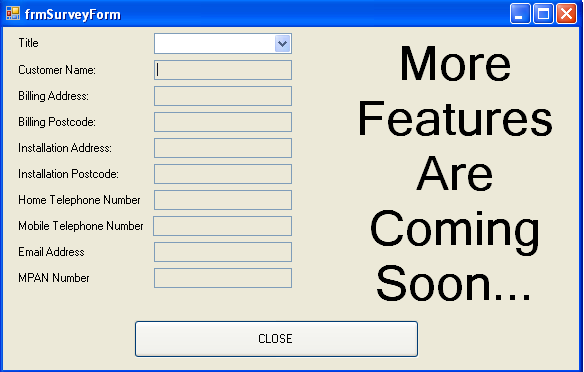
\includegraphics[scale=0.5]{frmSurveyForm_scrot}
	\makeatletter
\def\PY@reset{\let\PY@it=\relax \let\PY@bf=\relax%
    \let\PY@ul=\relax \let\PY@tc=\relax%
    \let\PY@bc=\relax \let\PY@ff=\relax}
\def\PY@tok#1{\csname PY@tok@#1\endcsname}
\def\PY@toks#1+{\ifx\relax#1\empty\else%
    \PY@tok{#1}\expandafter\PY@toks\fi}
\def\PY@do#1{\PY@bc{\PY@tc{\PY@ul{%
    \PY@it{\PY@bf{\PY@ff{#1}}}}}}}
\def\PY#1#2{\PY@reset\PY@toks#1+\relax+\PY@do{#2}}

\expandafter\def\csname PY@tok@gd\endcsname{\def\PY@tc##1{\textcolor[rgb]{0.63,0.00,0.00}{##1}}}
\expandafter\def\csname PY@tok@gu\endcsname{\let\PY@bf=\textbf\def\PY@tc##1{\textcolor[rgb]{0.50,0.00,0.50}{##1}}}
\expandafter\def\csname PY@tok@gt\endcsname{\def\PY@tc##1{\textcolor[rgb]{0.00,0.25,0.82}{##1}}}
\expandafter\def\csname PY@tok@gs\endcsname{\let\PY@bf=\textbf}
\expandafter\def\csname PY@tok@gr\endcsname{\def\PY@tc##1{\textcolor[rgb]{1.00,0.00,0.00}{##1}}}
\expandafter\def\csname PY@tok@cm\endcsname{\let\PY@it=\textit\def\PY@tc##1{\textcolor[rgb]{0.25,0.50,0.50}{##1}}}
\expandafter\def\csname PY@tok@vg\endcsname{\def\PY@tc##1{\textcolor[rgb]{0.10,0.09,0.49}{##1}}}
\expandafter\def\csname PY@tok@m\endcsname{\def\PY@tc##1{\textcolor[rgb]{0.40,0.40,0.40}{##1}}}
\expandafter\def\csname PY@tok@mh\endcsname{\def\PY@tc##1{\textcolor[rgb]{0.40,0.40,0.40}{##1}}}
\expandafter\def\csname PY@tok@go\endcsname{\def\PY@tc##1{\textcolor[rgb]{0.50,0.50,0.50}{##1}}}
\expandafter\def\csname PY@tok@ge\endcsname{\let\PY@it=\textit}
\expandafter\def\csname PY@tok@vc\endcsname{\def\PY@tc##1{\textcolor[rgb]{0.10,0.09,0.49}{##1}}}
\expandafter\def\csname PY@tok@il\endcsname{\def\PY@tc##1{\textcolor[rgb]{0.40,0.40,0.40}{##1}}}
\expandafter\def\csname PY@tok@cs\endcsname{\let\PY@it=\textit\def\PY@tc##1{\textcolor[rgb]{0.25,0.50,0.50}{##1}}}
\expandafter\def\csname PY@tok@cp\endcsname{\def\PY@tc##1{\textcolor[rgb]{0.74,0.48,0.00}{##1}}}
\expandafter\def\csname PY@tok@gi\endcsname{\def\PY@tc##1{\textcolor[rgb]{0.00,0.63,0.00}{##1}}}
\expandafter\def\csname PY@tok@gh\endcsname{\let\PY@bf=\textbf\def\PY@tc##1{\textcolor[rgb]{0.00,0.00,0.50}{##1}}}
\expandafter\def\csname PY@tok@ni\endcsname{\let\PY@bf=\textbf\def\PY@tc##1{\textcolor[rgb]{0.60,0.60,0.60}{##1}}}
\expandafter\def\csname PY@tok@nl\endcsname{\def\PY@tc##1{\textcolor[rgb]{0.63,0.63,0.00}{##1}}}
\expandafter\def\csname PY@tok@nn\endcsname{\let\PY@bf=\textbf\def\PY@tc##1{\textcolor[rgb]{0.00,0.00,1.00}{##1}}}
\expandafter\def\csname PY@tok@no\endcsname{\def\PY@tc##1{\textcolor[rgb]{0.53,0.00,0.00}{##1}}}
\expandafter\def\csname PY@tok@na\endcsname{\def\PY@tc##1{\textcolor[rgb]{0.49,0.56,0.16}{##1}}}
\expandafter\def\csname PY@tok@nb\endcsname{\def\PY@tc##1{\textcolor[rgb]{0.00,0.50,0.00}{##1}}}
\expandafter\def\csname PY@tok@nc\endcsname{\let\PY@bf=\textbf\def\PY@tc##1{\textcolor[rgb]{0.00,0.00,1.00}{##1}}}
\expandafter\def\csname PY@tok@nd\endcsname{\def\PY@tc##1{\textcolor[rgb]{0.67,0.13,1.00}{##1}}}
\expandafter\def\csname PY@tok@ne\endcsname{\let\PY@bf=\textbf\def\PY@tc##1{\textcolor[rgb]{0.82,0.25,0.23}{##1}}}
\expandafter\def\csname PY@tok@nf\endcsname{\def\PY@tc##1{\textcolor[rgb]{0.00,0.00,1.00}{##1}}}
\expandafter\def\csname PY@tok@si\endcsname{\let\PY@bf=\textbf\def\PY@tc##1{\textcolor[rgb]{0.73,0.40,0.53}{##1}}}
\expandafter\def\csname PY@tok@s2\endcsname{\def\PY@tc##1{\textcolor[rgb]{0.73,0.13,0.13}{##1}}}
\expandafter\def\csname PY@tok@vi\endcsname{\def\PY@tc##1{\textcolor[rgb]{0.10,0.09,0.49}{##1}}}
\expandafter\def\csname PY@tok@nt\endcsname{\let\PY@bf=\textbf\def\PY@tc##1{\textcolor[rgb]{0.00,0.50,0.00}{##1}}}
\expandafter\def\csname PY@tok@nv\endcsname{\def\PY@tc##1{\textcolor[rgb]{0.10,0.09,0.49}{##1}}}
\expandafter\def\csname PY@tok@s1\endcsname{\def\PY@tc##1{\textcolor[rgb]{0.73,0.13,0.13}{##1}}}
\expandafter\def\csname PY@tok@sh\endcsname{\def\PY@tc##1{\textcolor[rgb]{0.73,0.13,0.13}{##1}}}
\expandafter\def\csname PY@tok@sc\endcsname{\def\PY@tc##1{\textcolor[rgb]{0.73,0.13,0.13}{##1}}}
\expandafter\def\csname PY@tok@sx\endcsname{\def\PY@tc##1{\textcolor[rgb]{0.00,0.50,0.00}{##1}}}
\expandafter\def\csname PY@tok@bp\endcsname{\def\PY@tc##1{\textcolor[rgb]{0.00,0.50,0.00}{##1}}}
\expandafter\def\csname PY@tok@c1\endcsname{\let\PY@it=\textit\def\PY@tc##1{\textcolor[rgb]{0.25,0.50,0.50}{##1}}}
\expandafter\def\csname PY@tok@kc\endcsname{\let\PY@bf=\textbf\def\PY@tc##1{\textcolor[rgb]{0.00,0.50,0.00}{##1}}}
\expandafter\def\csname PY@tok@c\endcsname{\let\PY@it=\textit\def\PY@tc##1{\textcolor[rgb]{0.25,0.50,0.50}{##1}}}
\expandafter\def\csname PY@tok@mf\endcsname{\def\PY@tc##1{\textcolor[rgb]{0.40,0.40,0.40}{##1}}}
\expandafter\def\csname PY@tok@err\endcsname{\def\PY@bc##1{\setlength{\fboxsep}{0pt}\fcolorbox[rgb]{1.00,0.00,0.00}{1,1,1}{\strut ##1}}}
\expandafter\def\csname PY@tok@kd\endcsname{\let\PY@bf=\textbf\def\PY@tc##1{\textcolor[rgb]{0.00,0.50,0.00}{##1}}}
\expandafter\def\csname PY@tok@ss\endcsname{\def\PY@tc##1{\textcolor[rgb]{0.10,0.09,0.49}{##1}}}
\expandafter\def\csname PY@tok@sr\endcsname{\def\PY@tc##1{\textcolor[rgb]{0.73,0.40,0.53}{##1}}}
\expandafter\def\csname PY@tok@mo\endcsname{\def\PY@tc##1{\textcolor[rgb]{0.40,0.40,0.40}{##1}}}
\expandafter\def\csname PY@tok@kn\endcsname{\let\PY@bf=\textbf\def\PY@tc##1{\textcolor[rgb]{0.00,0.50,0.00}{##1}}}
\expandafter\def\csname PY@tok@mi\endcsname{\def\PY@tc##1{\textcolor[rgb]{0.40,0.40,0.40}{##1}}}
\expandafter\def\csname PY@tok@gp\endcsname{\let\PY@bf=\textbf\def\PY@tc##1{\textcolor[rgb]{0.00,0.00,0.50}{##1}}}
\expandafter\def\csname PY@tok@o\endcsname{\def\PY@tc##1{\textcolor[rgb]{0.40,0.40,0.40}{##1}}}
\expandafter\def\csname PY@tok@kr\endcsname{\let\PY@bf=\textbf\def\PY@tc##1{\textcolor[rgb]{0.00,0.50,0.00}{##1}}}
\expandafter\def\csname PY@tok@s\endcsname{\def\PY@tc##1{\textcolor[rgb]{0.73,0.13,0.13}{##1}}}
\expandafter\def\csname PY@tok@kp\endcsname{\def\PY@tc##1{\textcolor[rgb]{0.00,0.50,0.00}{##1}}}
\expandafter\def\csname PY@tok@w\endcsname{\def\PY@tc##1{\textcolor[rgb]{0.73,0.73,0.73}{##1}}}
\expandafter\def\csname PY@tok@kt\endcsname{\def\PY@tc##1{\textcolor[rgb]{0.69,0.00,0.25}{##1}}}
\expandafter\def\csname PY@tok@ow\endcsname{\let\PY@bf=\textbf\def\PY@tc##1{\textcolor[rgb]{0.67,0.13,1.00}{##1}}}
\expandafter\def\csname PY@tok@sb\endcsname{\def\PY@tc##1{\textcolor[rgb]{0.73,0.13,0.13}{##1}}}
\expandafter\def\csname PY@tok@k\endcsname{\let\PY@bf=\textbf\def\PY@tc##1{\textcolor[rgb]{0.00,0.50,0.00}{##1}}}
\expandafter\def\csname PY@tok@se\endcsname{\let\PY@bf=\textbf\def\PY@tc##1{\textcolor[rgb]{0.73,0.40,0.13}{##1}}}
\expandafter\def\csname PY@tok@sd\endcsname{\let\PY@it=\textit\def\PY@tc##1{\textcolor[rgb]{0.73,0.13,0.13}{##1}}}

\def\PYZbs{\char`\\}
\def\PYZus{\char`\_}
\def\PYZob{\char`\{}
\def\PYZcb{\char`\}}
\def\PYZca{\char`\^}
\def\PYZam{\char`\&}
\def\PYZlt{\char`\<}
\def\PYZgt{\char`\>}
\def\PYZsh{\char`\#}
\def\PYZpc{\char`\%}
\def\PYZdl{\char`\$}
\def\PYZti{\char`\~}
% for compatibility with earlier versions
\def\PYZat{@}
\def\PYZlb{[}
\def\PYZrb{]}
\makeatother

\begin{Verbatim}[commandchars=\\\{\}]
\PY{k}{Imports} \PY{n+nn}{System.Data}
\PY{k}{Imports} \PY{n+nn}{System.Data.OleDb}
\PY{k}{Public} \PY{k}{Class} \PY{n+nc}{frmSurveyForm}

    \PY{k}{Public} \PY{n}{accConnection} \PY{o+ow}{As} \PY{k}{New} \PY{n}{OleDbConnection}

    \PY{k}{Private} \PY{k}{Sub} \PY{n+nf}{frmSurveyForm\PYZus{}Load}\PY{p}{(}\PY{k}{ByVal} \PY{n}{sender} \PY{o+ow}{As} \PY{n}{System}\PY{p}{.}\PY{n}{Object}\PY{p}{,} \PY{n}{\PYZus{}}
                                   \PY{k}{ByVal} \PY{n}{e} \PY{o+ow}{As} \PY{n}{System}\PY{p}{.}\PY{n}{EventArgs}\PY{p}{)} \PY{k}{Handles} \PY{k}{MyBase}\PY{p}{.}\PY{n}{Load}
        \PY{c}{'All this does, for now, is display the selected customer details.}
        \PY{c}{'In the future, full survey details will be able to be entered by}
        \PY{c}{'the user, however at this moment I cannot implement this due to }
        \PY{c}{'time constraints, so it will be implemented in after-development.}
        \PY{c}{'To show this to the user when he or she hunts around, there}
        \PY{c}{'exists a placeholder text label that states that features are}
        \PY{c}{'coming soon.}

        \PY{k}{If} \PY{n}{frmLoginForm}\PY{p}{.}\PY{n}{accConnection}\PY{p}{.}\PY{n}{State} \PY{o}{\PYZlt{}\PYZgt{}} \PY{n}{ConnectionState}\PY{p}{.}\PY{n}{Open} \PY{k}{Then}
            \PY{n}{frmLoginForm}\PY{p}{.}\PY{n}{accConnection}\PY{p}{.}\PY{n}{Open}\PY{p}{(}\PY{p}{)}
        \PY{k}{End} \PY{k}{If}

        \PY{n}{accConnection} \PY{o}{=} \PY{n}{frmLoginForm}\PY{p}{.}\PY{n}{accConnection}
        \PY{c}{'Input customer name from the other form and attribute it to CN.}
        \PY{k}{Dim} \PY{n}{cn} \PY{o+ow}{As} \PY{k+kt}{String} \PY{o}{=} \PY{n}{frmReportSurvey}\PY{p}{.}\PY{n}{txtcbReportSurvey}\PY{p}{.}\PY{n}{SelectedItem}
        \PY{k}{Dim} \PY{n}{cmdString} \PY{o+ow}{As} \PY{k+kt}{String} \PY{o}{=} \PY{l+s}{"}\PY{l+s}{SELECT * FROM Customer WHERE cust\PYZus{}name = '}\PY{l+s}{"} \PY{o}{\PYZam{}} \PY{n}{cn} \PY{o}{\PYZam{}} \PY{l+s}{"}\PY{l+s}{'}\PY{l+s}{"}
        \PY{k}{Dim} \PY{n}{accCommand} \PY{o+ow}{As} \PY{k}{New} \PY{n}{OleDbCommand}
        \PY{k}{Dim} \PY{n}{da} \PY{o+ow}{As} \PY{k}{New} \PY{n}{OleDbDataAdapter}\PY{p}{(}\PY{n}{cmdString}\PY{p}{,} \PY{n}{accConnection}\PY{p}{)}
        \PY{k}{Dim} \PY{n}{ds} \PY{o+ow}{As} \PY{k}{New} \PY{n}{DataSet}

        \PY{n}{da}\PY{p}{.}\PY{n}{Fill}\PY{p}{(}\PY{n}{ds}\PY{p}{,} \PY{l+s}{"}\PY{l+s}{Customer}\PY{l+s}{"}\PY{p}{)}

        \PY{k}{Dim} \PY{n}{dt} \PY{o+ow}{As} \PY{n}{DataTable} \PY{o}{=} \PY{n}{ds}\PY{p}{.}\PY{n}{Tables}\PY{p}{(}\PY{l+m+mi}{0}\PY{p}{)}
        \PY{k}{Dim} \PY{n}{dr} \PY{o+ow}{As} \PY{n}{DataRow} \PY{c}{'\PYZlt{}- This is redundant.sss}

        \PY{c}{'Populate the textboxes in the form with existing customer details.}
        \PY{c}{'All the customer data text boxes are read-only to avoid data error:}
        \PY{c}{'to edit those, edit the customer details directly, then come back.}

        \PY{c}{'Populate the customer name textbox with the customer name}
        \PY{c}{'from the other form, before getting info from db about others.}
        \PY{n}{txtscn}\PY{p}{.}\PY{n}{Text} \PY{o}{=} \PY{n}{cn}
        \PY{k}{If} \PY{n}{ds}\PY{p}{.}\PY{n}{Tables}\PY{p}{(}\PY{l+m+mi}{0}\PY{p}{)}\PY{p}{.}\PY{n}{Rows}\PY{p}{.}\PY{n}{Count} \PY{o}{\PYZlt{}\PYZgt{}} \PY{l+m+mi}{0} \PY{k}{Then}
            \PY{n}{cbsct}\PY{p}{.}\PY{n}{Text} \PY{o}{=} \PY{n}{ds}\PY{p}{.}\PY{n}{Tables}\PY{p}{(}\PY{l+m+mi}{0}\PY{p}{)}\PY{p}{.}\PY{n}{Rows}\PY{p}{(}\PY{l+m+mi}{0}\PY{p}{)}\PY{p}{.}\PY{n}{Item}\PY{p}{(}\PY{l+s}{"}\PY{l+s}{cust\PYZus{}title}\PY{l+s}{"}\PY{p}{)}
            \PY{n}{txtscba}\PY{p}{.}\PY{n}{Text} \PY{o}{=} \PY{n}{ds}\PY{p}{.}\PY{n}{Tables}\PY{p}{(}\PY{l+m+mi}{0}\PY{p}{)}\PY{p}{.}\PY{n}{Rows}\PY{p}{(}\PY{l+m+mi}{0}\PY{p}{)}\PY{p}{.}\PY{n}{Item}\PY{p}{(}\PY{l+s}{"}\PY{l+s}{cust\PYZus{}billaddress}\PY{l+s}{"}\PY{p}{)}
            \PY{n}{txtscbp}\PY{p}{.}\PY{n}{Text} \PY{o}{=} \PY{n}{ds}\PY{p}{.}\PY{n}{Tables}\PY{p}{(}\PY{l+m+mi}{0}\PY{p}{)}\PY{p}{.}\PY{n}{Rows}\PY{p}{(}\PY{l+m+mi}{0}\PY{p}{)}\PY{p}{.}\PY{n}{Item}\PY{p}{(}\PY{l+s}{"}\PY{l+s}{cust\PYZus{}billpostcode}\PY{l+s}{"}\PY{p}{)}
            \PY{n}{txtscia}\PY{p}{.}\PY{n}{Text} \PY{o}{=} \PY{n}{ds}\PY{p}{.}\PY{n}{Tables}\PY{p}{(}\PY{l+m+mi}{0}\PY{p}{)}\PY{p}{.}\PY{n}{Rows}\PY{p}{(}\PY{l+m+mi}{0}\PY{p}{)}\PY{p}{.}\PY{n}{Item}\PY{p}{(}\PY{l+s}{"}\PY{l+s}{cust\PYZus{}instaddress}\PY{l+s}{"}\PY{p}{)}
            \PY{n}{txtscip}\PY{p}{.}\PY{n}{Text} \PY{o}{=} \PY{n}{ds}\PY{p}{.}\PY{n}{Tables}\PY{p}{(}\PY{l+m+mi}{0}\PY{p}{)}\PY{p}{.}\PY{n}{Rows}\PY{p}{(}\PY{l+m+mi}{0}\PY{p}{)}\PY{p}{.}\PY{n}{Item}\PY{p}{(}\PY{l+s}{"}\PY{l+s}{cust\PYZus{}instpostcode}\PY{l+s}{"}\PY{p}{)}
            \PY{n}{txtschtn}\PY{p}{.}\PY{n}{Text} \PY{o}{=} \PY{n}{ds}\PY{p}{.}\PY{n}{Tables}\PY{p}{(}\PY{l+m+mi}{0}\PY{p}{)}\PY{p}{.}\PY{n}{Rows}\PY{p}{(}\PY{l+m+mi}{0}\PY{p}{)}\PY{p}{.}\PY{n}{Item}\PY{p}{(}\PY{l+s}{"}\PY{l+s}{cust\PYZus{}hometelno}\PY{l+s}{"}\PY{p}{)}
            \PY{n}{txtscmtn}\PY{p}{.}\PY{n}{Text} \PY{o}{=} \PY{n}{ds}\PY{p}{.}\PY{n}{Tables}\PY{p}{(}\PY{l+m+mi}{0}\PY{p}{)}\PY{p}{.}\PY{n}{Rows}\PY{p}{(}\PY{l+m+mi}{0}\PY{p}{)}\PY{p}{.}\PY{n}{Item}\PY{p}{(}\PY{l+s}{"}\PY{l+s}{cust\PYZus{}mobtelno}\PY{l+s}{"}\PY{p}{)}
            \PY{n}{txtscmpan}\PY{p}{.}\PY{n}{Text} \PY{o}{=} \PY{n}{ds}\PY{p}{.}\PY{n}{Tables}\PY{p}{(}\PY{l+m+mi}{0}\PY{p}{)}\PY{p}{.}\PY{n}{Rows}\PY{p}{(}\PY{l+m+mi}{0}\PY{p}{)}\PY{p}{.}\PY{n}{Item}\PY{p}{(}\PY{l+s}{"}\PY{l+s}{cust\PYZus{}mpan}\PY{l+s}{"}\PY{p}{)}
            \PY{n}{txtscea}\PY{p}{.}\PY{n}{Text} \PY{o}{=} \PY{n}{ds}\PY{p}{.}\PY{n}{Tables}\PY{p}{(}\PY{l+m+mi}{0}\PY{p}{)}\PY{p}{.}\PY{n}{Rows}\PY{p}{(}\PY{l+m+mi}{0}\PY{p}{)}\PY{p}{.}\PY{n}{Item}\PY{p}{(}\PY{l+s}{"}\PY{l+s}{cust\PYZus{}email}\PY{l+s}{"}\PY{p}{)}
        \PY{k}{End} \PY{k}{If}

        \PY{n}{accCommand}\PY{p}{.}\PY{n}{Connection} \PY{o}{=} \PY{n}{frmLoginForm}\PY{p}{.}\PY{n}{accConnection}
        \PY{n}{accCommand}\PY{p}{.}\PY{n}{CommandType} \PY{o}{=} \PY{n}{CommandType}\PY{p}{.}\PY{n}{Text}
        \PY{n}{accCommand}\PY{p}{.}\PY{n}{CommandText} \PY{o}{=} \PY{n}{cmdString}

    \PY{k}{End} \PY{k}{Sub}

    \PY{k}{Private} \PY{k}{Sub} \PY{n+nf}{btnClose\PYZus{}Click}\PY{p}{(}\PY{k}{ByVal} \PY{n}{sender} \PY{o+ow}{As} \PY{n}{System}\PY{p}{.}\PY{n}{Object}\PY{p}{,} \PY{n}{\PYZus{}}
                               \PY{k}{ByVal} \PY{n}{e} \PY{o+ow}{As} \PY{n}{System}\PY{p}{.}\PY{n}{EventArgs}\PY{p}{)} \PY{k}{Handles} \PY{n}{btnClose}\PY{p}{.}\PY{n}{Click}
        \PY{k}{Me}\PY{p}{.}\PY{n}{Close}\PY{p}{(}\PY{p}{)}
        \PY{n}{frmReportSurvey}\PY{p}{.}\PY{n}{Show}\PY{p}{(}\PY{p}{)}
    \PY{k}{End} \PY{k}{Sub}
\PY{k}{End} \PY{k}{Class}
\end{Verbatim}

	
\subsection{frmSwankyCode}
		I have not included a screenshot here as it would provide no information whatsoever due to the form being blank and serving no function other than a home for stray but useful pieces of code.
	\makeatletter
\def\PY@reset{\let\PY@it=\relax \let\PY@bf=\relax%
    \let\PY@ul=\relax \let\PY@tc=\relax%
    \let\PY@bc=\relax \let\PY@ff=\relax}
\def\PY@tok#1{\csname PY@tok@#1\endcsname}
\def\PY@toks#1+{\ifx\relax#1\empty\else%
    \PY@tok{#1}\expandafter\PY@toks\fi}
\def\PY@do#1{\PY@bc{\PY@tc{\PY@ul{%
    \PY@it{\PY@bf{\PY@ff{#1}}}}}}}
\def\PY#1#2{\PY@reset\PY@toks#1+\relax+\PY@do{#2}}

\expandafter\def\csname PY@tok@gd\endcsname{\def\PY@tc##1{\textcolor[rgb]{0.63,0.00,0.00}{##1}}}
\expandafter\def\csname PY@tok@gu\endcsname{\let\PY@bf=\textbf\def\PY@tc##1{\textcolor[rgb]{0.50,0.00,0.50}{##1}}}
\expandafter\def\csname PY@tok@gt\endcsname{\def\PY@tc##1{\textcolor[rgb]{0.00,0.25,0.82}{##1}}}
\expandafter\def\csname PY@tok@gs\endcsname{\let\PY@bf=\textbf}
\expandafter\def\csname PY@tok@gr\endcsname{\def\PY@tc##1{\textcolor[rgb]{1.00,0.00,0.00}{##1}}}
\expandafter\def\csname PY@tok@cm\endcsname{\let\PY@it=\textit\def\PY@tc##1{\textcolor[rgb]{0.25,0.50,0.50}{##1}}}
\expandafter\def\csname PY@tok@vg\endcsname{\def\PY@tc##1{\textcolor[rgb]{0.10,0.09,0.49}{##1}}}
\expandafter\def\csname PY@tok@m\endcsname{\def\PY@tc##1{\textcolor[rgb]{0.40,0.40,0.40}{##1}}}
\expandafter\def\csname PY@tok@mh\endcsname{\def\PY@tc##1{\textcolor[rgb]{0.40,0.40,0.40}{##1}}}
\expandafter\def\csname PY@tok@go\endcsname{\def\PY@tc##1{\textcolor[rgb]{0.50,0.50,0.50}{##1}}}
\expandafter\def\csname PY@tok@ge\endcsname{\let\PY@it=\textit}
\expandafter\def\csname PY@tok@vc\endcsname{\def\PY@tc##1{\textcolor[rgb]{0.10,0.09,0.49}{##1}}}
\expandafter\def\csname PY@tok@il\endcsname{\def\PY@tc##1{\textcolor[rgb]{0.40,0.40,0.40}{##1}}}
\expandafter\def\csname PY@tok@cs\endcsname{\let\PY@it=\textit\def\PY@tc##1{\textcolor[rgb]{0.25,0.50,0.50}{##1}}}
\expandafter\def\csname PY@tok@cp\endcsname{\def\PY@tc##1{\textcolor[rgb]{0.74,0.48,0.00}{##1}}}
\expandafter\def\csname PY@tok@gi\endcsname{\def\PY@tc##1{\textcolor[rgb]{0.00,0.63,0.00}{##1}}}
\expandafter\def\csname PY@tok@gh\endcsname{\let\PY@bf=\textbf\def\PY@tc##1{\textcolor[rgb]{0.00,0.00,0.50}{##1}}}
\expandafter\def\csname PY@tok@ni\endcsname{\let\PY@bf=\textbf\def\PY@tc##1{\textcolor[rgb]{0.60,0.60,0.60}{##1}}}
\expandafter\def\csname PY@tok@nl\endcsname{\def\PY@tc##1{\textcolor[rgb]{0.63,0.63,0.00}{##1}}}
\expandafter\def\csname PY@tok@nn\endcsname{\let\PY@bf=\textbf\def\PY@tc##1{\textcolor[rgb]{0.00,0.00,1.00}{##1}}}
\expandafter\def\csname PY@tok@no\endcsname{\def\PY@tc##1{\textcolor[rgb]{0.53,0.00,0.00}{##1}}}
\expandafter\def\csname PY@tok@na\endcsname{\def\PY@tc##1{\textcolor[rgb]{0.49,0.56,0.16}{##1}}}
\expandafter\def\csname PY@tok@nb\endcsname{\def\PY@tc##1{\textcolor[rgb]{0.00,0.50,0.00}{##1}}}
\expandafter\def\csname PY@tok@nc\endcsname{\let\PY@bf=\textbf\def\PY@tc##1{\textcolor[rgb]{0.00,0.00,1.00}{##1}}}
\expandafter\def\csname PY@tok@nd\endcsname{\def\PY@tc##1{\textcolor[rgb]{0.67,0.13,1.00}{##1}}}
\expandafter\def\csname PY@tok@ne\endcsname{\let\PY@bf=\textbf\def\PY@tc##1{\textcolor[rgb]{0.82,0.25,0.23}{##1}}}
\expandafter\def\csname PY@tok@nf\endcsname{\def\PY@tc##1{\textcolor[rgb]{0.00,0.00,1.00}{##1}}}
\expandafter\def\csname PY@tok@si\endcsname{\let\PY@bf=\textbf\def\PY@tc##1{\textcolor[rgb]{0.73,0.40,0.53}{##1}}}
\expandafter\def\csname PY@tok@s2\endcsname{\def\PY@tc##1{\textcolor[rgb]{0.73,0.13,0.13}{##1}}}
\expandafter\def\csname PY@tok@vi\endcsname{\def\PY@tc##1{\textcolor[rgb]{0.10,0.09,0.49}{##1}}}
\expandafter\def\csname PY@tok@nt\endcsname{\let\PY@bf=\textbf\def\PY@tc##1{\textcolor[rgb]{0.00,0.50,0.00}{##1}}}
\expandafter\def\csname PY@tok@nv\endcsname{\def\PY@tc##1{\textcolor[rgb]{0.10,0.09,0.49}{##1}}}
\expandafter\def\csname PY@tok@s1\endcsname{\def\PY@tc##1{\textcolor[rgb]{0.73,0.13,0.13}{##1}}}
\expandafter\def\csname PY@tok@sh\endcsname{\def\PY@tc##1{\textcolor[rgb]{0.73,0.13,0.13}{##1}}}
\expandafter\def\csname PY@tok@sc\endcsname{\def\PY@tc##1{\textcolor[rgb]{0.73,0.13,0.13}{##1}}}
\expandafter\def\csname PY@tok@sx\endcsname{\def\PY@tc##1{\textcolor[rgb]{0.00,0.50,0.00}{##1}}}
\expandafter\def\csname PY@tok@bp\endcsname{\def\PY@tc##1{\textcolor[rgb]{0.00,0.50,0.00}{##1}}}
\expandafter\def\csname PY@tok@c1\endcsname{\let\PY@it=\textit\def\PY@tc##1{\textcolor[rgb]{0.25,0.50,0.50}{##1}}}
\expandafter\def\csname PY@tok@kc\endcsname{\let\PY@bf=\textbf\def\PY@tc##1{\textcolor[rgb]{0.00,0.50,0.00}{##1}}}
\expandafter\def\csname PY@tok@c\endcsname{\let\PY@it=\textit\def\PY@tc##1{\textcolor[rgb]{0.25,0.50,0.50}{##1}}}
\expandafter\def\csname PY@tok@mf\endcsname{\def\PY@tc##1{\textcolor[rgb]{0.40,0.40,0.40}{##1}}}
\expandafter\def\csname PY@tok@err\endcsname{\def\PY@bc##1{\setlength{\fboxsep}{0pt}\fcolorbox[rgb]{1.00,0.00,0.00}{1,1,1}{\strut ##1}}}
\expandafter\def\csname PY@tok@kd\endcsname{\let\PY@bf=\textbf\def\PY@tc##1{\textcolor[rgb]{0.00,0.50,0.00}{##1}}}
\expandafter\def\csname PY@tok@ss\endcsname{\def\PY@tc##1{\textcolor[rgb]{0.10,0.09,0.49}{##1}}}
\expandafter\def\csname PY@tok@sr\endcsname{\def\PY@tc##1{\textcolor[rgb]{0.73,0.40,0.53}{##1}}}
\expandafter\def\csname PY@tok@mo\endcsname{\def\PY@tc##1{\textcolor[rgb]{0.40,0.40,0.40}{##1}}}
\expandafter\def\csname PY@tok@kn\endcsname{\let\PY@bf=\textbf\def\PY@tc##1{\textcolor[rgb]{0.00,0.50,0.00}{##1}}}
\expandafter\def\csname PY@tok@mi\endcsname{\def\PY@tc##1{\textcolor[rgb]{0.40,0.40,0.40}{##1}}}
\expandafter\def\csname PY@tok@gp\endcsname{\let\PY@bf=\textbf\def\PY@tc##1{\textcolor[rgb]{0.00,0.00,0.50}{##1}}}
\expandafter\def\csname PY@tok@o\endcsname{\def\PY@tc##1{\textcolor[rgb]{0.40,0.40,0.40}{##1}}}
\expandafter\def\csname PY@tok@kr\endcsname{\let\PY@bf=\textbf\def\PY@tc##1{\textcolor[rgb]{0.00,0.50,0.00}{##1}}}
\expandafter\def\csname PY@tok@s\endcsname{\def\PY@tc##1{\textcolor[rgb]{0.73,0.13,0.13}{##1}}}
\expandafter\def\csname PY@tok@kp\endcsname{\def\PY@tc##1{\textcolor[rgb]{0.00,0.50,0.00}{##1}}}
\expandafter\def\csname PY@tok@w\endcsname{\def\PY@tc##1{\textcolor[rgb]{0.73,0.73,0.73}{##1}}}
\expandafter\def\csname PY@tok@kt\endcsname{\def\PY@tc##1{\textcolor[rgb]{0.69,0.00,0.25}{##1}}}
\expandafter\def\csname PY@tok@ow\endcsname{\let\PY@bf=\textbf\def\PY@tc##1{\textcolor[rgb]{0.67,0.13,1.00}{##1}}}
\expandafter\def\csname PY@tok@sb\endcsname{\def\PY@tc##1{\textcolor[rgb]{0.73,0.13,0.13}{##1}}}
\expandafter\def\csname PY@tok@k\endcsname{\let\PY@bf=\textbf\def\PY@tc##1{\textcolor[rgb]{0.00,0.50,0.00}{##1}}}
\expandafter\def\csname PY@tok@se\endcsname{\let\PY@bf=\textbf\def\PY@tc##1{\textcolor[rgb]{0.73,0.40,0.13}{##1}}}
\expandafter\def\csname PY@tok@sd\endcsname{\let\PY@it=\textit\def\PY@tc##1{\textcolor[rgb]{0.73,0.13,0.13}{##1}}}

\def\PYZbs{\char`\\}
\def\PYZus{\char`\_}
\def\PYZob{\char`\{}
\def\PYZcb{\char`\}}
\def\PYZca{\char`\^}
\def\PYZam{\char`\&}
\def\PYZlt{\char`\<}
\def\PYZgt{\char`\>}
\def\PYZsh{\char`\#}
\def\PYZpc{\char`\%}
\def\PYZdl{\char`\$}
\def\PYZti{\char`\~}
% for compatibility with earlier versions
\def\PYZat{@}
\def\PYZlb{[}
\def\PYZrb{]}
\makeatother

\begin{Verbatim}[commandchars=\\\{\}]
\PY{k}{Imports} \PY{n+nn}{Microsoft.Office.Core}
\PY{k}{Imports} \PY{n+nn}{Microsoft.Office.Interop}
\PY{k}{Imports} \PY{n+nn}{Microsoft.Office.Interop.Word}

\PY{k}{Public} \PY{k}{Class} \PY{n+nc}{frmSwankyCode}

    \PY{c}{'This is a form because I couldn't work out how to make it work any}
    \PY{c}{'other way.}

    \PY{c}{'This is where all the code goes that is referenced from other subs}
    \PY{c}{'in other forms, to save space and attempt to minimise repetition.}

    \PY{k}{Public} \PY{k}{Sub} \PY{n+nf}{CheckAdditions}\PY{p}{(}\PY{k}{ByVal} \PY{n}{intInsert} \PY{o+ow}{As} \PY{k+kt}{Integer}\PY{p}{,} \PY{n}{\PYZus{}}
                              \PY{k}{ByRef} \PY{n}{btnSave} \PY{o+ow}{As} \PY{n}{Button}\PY{p}{)}

        \PY{k}{If} \PY{n}{intInsert} \PY{o}{=} \PY{l+m+mi}{0} \PY{k}{Then}
            \PY{n}{MsgBox}\PY{p}{(}\PY{l+s}{"}\PY{l+s}{Data insertion failed.}\PY{l+s}{"}\PY{p}{)}
        \PY{k}{Else}
            \PY{c}{'Assume it went through OK and disable the Save button to}
            \PY{c}{'guard against duplication.}
            \PY{n}{btnSave}\PY{p}{.}\PY{n}{Enabled} \PY{o}{=} \PY{k}{False}
        \PY{k}{End} \PY{k}{If}

    \PY{k}{End} \PY{k}{Sub}

    \PY{k}{Public} \PY{k}{Sub} \PY{n+nf}{WordInvoiceAutomationMagic}\PY{p}{(}\PY{k}{ByVal} \PY{n}{ict} \PY{o+ow}{As} \PY{k+kt}{String}\PY{p}{,} \PY{k}{ByVal} \PY{n}{icn} \PY{o+ow}{As} \PY{k+kt}{String}\PY{p}{,} \PY{n}{\PYZus{}}
                                   \PY{k}{ByVal} \PY{n}{ica} \PY{o+ow}{As} \PY{k+kt}{String}\PY{p}{,} \PY{k}{ByVal} \PY{n}{icp} \PY{o+ow}{As} \PY{k+kt}{String}\PY{p}{)}

        \PY{c}{'THIS CODE SATISFIES SPECIFIC OBJECTIVE 14.}

        \PY{k}{Dim} \PY{n}{oWord} \PY{o+ow}{As} \PY{n}{Word}\PY{p}{.}\PY{n}{Application}
        \PY{k}{Dim} \PY{n}{oDoc} \PY{o+ow}{As} \PY{n}{Word}\PY{p}{.}\PY{n}{Document}
        \PY{k}{Dim} \PY{n}{CustAddressStuff} \PY{o+ow}{As} \PY{n}{Word}\PY{p}{.}\PY{n}{Paragraph}
        \PY{k}{Dim} \PY{n}{CustInvoiceHeader} \PY{o+ow}{As} \PY{n}{Word}\PY{p}{.}\PY{n}{Paragraph}

        \PY{c}{'Start Word and open the document.}
        \PY{c}{'This is object stuff that I don't understand, but it was found on}
        \PY{c}{'a Microsoft doc, and the other stuff I tried didn't work, so I}
        \PY{c}{'used it.}
        \PY{n}{oWord} \PY{o}{=} \PY{n}{CreateObject}\PY{p}{(}\PY{l+s}{"}\PY{l+s}{Word.Application}\PY{l+s}{"}\PY{p}{)}
        \PY{n}{oWord}\PY{p}{.}\PY{n}{Visible} \PY{o}{=} \PY{k}{True}
        \PY{n}{oDoc} \PY{o}{=} \PY{n}{oWord}\PY{p}{.}\PY{n}{Documents}\PY{p}{.}\PY{n}{Add}

        \PY{c}{'Insert the customer billing address stuff.}
        \PY{n}{CustAddressStuff} \PY{o}{=} \PY{n}{oDoc}\PY{p}{.}\PY{n}{Content}\PY{p}{.}\PY{n}{Paragraphs}\PY{p}{.}\PY{n}{Add}
        \PY{n}{CustAddressStuff}\PY{p}{.}\PY{n}{Range}\PY{p}{.}\PY{n}{Text} \PY{o}{=} \PY{n}{ict} \PY{o}{\PYZam{}} \PY{l+s}{"}\PY{l+s}{ }\PY{l+s}{"} \PY{o}{\PYZam{}} \PY{n}{icn} \PY{o}{\PYZam{}} \PY{n}{Chr}\PY{p}{(}\PY{l+m+mi}{11}\PY{p}{)} \PY{o}{\PYZam{}} \PY{n}{ica} \PY{n}{\PYZus{}}
                                      \PY{o}{\PYZam{}} \PY{n}{Chr}\PY{p}{(}\PY{l+m+mi}{11}\PY{p}{)} \PY{o}{\PYZam{}} \PY{n}{icp} \PY{o}{\PYZam{}} \PY{n}{Chr}\PY{p}{(}\PY{l+m+mi}{11}\PY{p}{)}
        \PY{n}{CustAddressStuff}\PY{p}{.}\PY{n}{Range}\PY{p}{.}\PY{n}{ParagraphFormat}\PY{p}{.}\PY{n}{Alignment} \PY{o}{=} \PY{n}{\PYZus{}}
            \PY{n}{Word}\PY{p}{.}\PY{n}{WdParagraphAlignment}\PY{p}{.}\PY{n}{wdAlignParagraphRight}
        \PY{n}{CustAddressStuff}\PY{p}{.}\PY{n}{Range}\PY{p}{.}\PY{n}{Font}\PY{p}{.}\PY{n}{Bold} \PY{o}{=} \PY{k}{False}

        \PY{c}{'Sort out the spacing afterwards.}
        \PY{n}{CustAddressStuff}\PY{p}{.}\PY{n}{Format}\PY{p}{.}\PY{n}{SpaceAfter} \PY{o}{=} \PY{l+m+mi}{4}
        \PY{n}{CustAddressStuff}\PY{p}{.}\PY{n}{Range}\PY{p}{.}\PY{n}{InsertParagraphAfter}\PY{p}{(}\PY{p}{)}

        \PY{c}{'Now, after the spacing, the INVOICE header, centred.}
        \PY{n}{CustInvoiceHeader} \PY{o}{=} \PY{n}{\PYZus{}}
            \PY{n}{oDoc}\PY{p}{.}\PY{n}{Content}\PY{p}{.}\PY{n}{Paragraphs}\PY{p}{.}\PY{n}{Add}\PY{p}{(}\PY{n}{oDoc}\PY{p}{.}\PY{n}{Bookmarks}\PY{p}{.}\PY{n}{Item}\PY{p}{(}\PY{l+s}{"}\PY{l+s}{\PYZbs{}endofdoc}\PY{l+s}{"}\PY{p}{)}\PY{p}{.}\PY{n}{Range}\PY{p}{)}
        \PY{n}{CustInvoiceHeader}\PY{p}{.}\PY{n}{Range}\PY{p}{.}\PY{n}{Text} \PY{o}{=} \PY{l+s}{"}\PY{l+s}{INVOICE}\PY{l+s}{"}
        \PY{n}{CustInvoiceHeader}\PY{p}{.}\PY{n}{Range}\PY{p}{.}\PY{n}{ParagraphFormat}\PY{p}{.}\PY{n}{Alignment} \PY{o}{=} \PY{n}{\PYZus{}}
            \PY{n}{Word}\PY{p}{.}\PY{n}{WdParagraphAlignment}\PY{p}{.}\PY{n}{wdAlignParagraphCenter}
        \PY{n}{CustInvoiceHeader}\PY{p}{.}\PY{n}{Range}\PY{p}{.}\PY{n}{Font}\PY{p}{.}\PY{n}{Size} \PY{o}{=} \PY{l+m+mi}{22}
        \PY{n}{CustInvoiceHeader}\PY{p}{.}\PY{n}{Range}\PY{p}{.}\PY{n}{Font}\PY{p}{.}\PY{n}{Bold} \PY{o}{=} \PY{k}{True}

    \PY{k}{End} \PY{k}{Sub}

    \PY{k}{Public} \PY{k}{Sub} \PY{n+nf}{WordQuotationAutomationMagic}\PY{p}{(}\PY{k}{ByVal} \PY{n}{qct} \PY{o+ow}{As} \PY{k+kt}{String}\PY{p}{,} \PY{k}{ByVal} \PY{n}{qcn} \PY{o+ow}{As} \PY{k+kt}{String}\PY{p}{,} \PY{n}{\PYZus{}}
                                   \PY{k}{ByVal} \PY{n}{qca} \PY{o+ow}{As} \PY{k+kt}{String}\PY{p}{,} \PY{k}{ByVal} \PY{n}{qcp} \PY{o+ow}{As} \PY{k+kt}{String}\PY{p}{)}

        \PY{c}{'THIS CODE SATISFIES SPECIFIC OBJECTIVE 14.}

        \PY{k}{Dim} \PY{n}{oWord} \PY{o+ow}{As} \PY{n}{Word}\PY{p}{.}\PY{n}{Application}
        \PY{k}{Dim} \PY{n}{oDoc} \PY{o+ow}{As} \PY{n}{Word}\PY{p}{.}\PY{n}{Document}
        \PY{k}{Dim} \PY{n}{CustAddressStuff} \PY{o+ow}{As} \PY{n}{Word}\PY{p}{.}\PY{n}{Paragraph}
        \PY{k}{Dim} \PY{n}{CustQuotationHeader} \PY{o+ow}{As} \PY{n}{Word}\PY{p}{.}\PY{n}{Paragraph}

        \PY{c}{'Start Word and open the document.}
        \PY{c}{'This is object stuff that I don't understand, but it was found on}
        \PY{c}{'a Microsoft doc, and the other stuff I tried didn't work, so I}
        \PY{c}{'used it.}
        \PY{n}{oWord} \PY{o}{=} \PY{n}{CreateObject}\PY{p}{(}\PY{l+s}{"}\PY{l+s}{Word.Application}\PY{l+s}{"}\PY{p}{)}
        \PY{n}{oWord}\PY{p}{.}\PY{n}{Visible} \PY{o}{=} \PY{k}{True}
        \PY{n}{oDoc} \PY{o}{=} \PY{n}{oWord}\PY{p}{.}\PY{n}{Documents}\PY{p}{.}\PY{n}{Add}

        \PY{c}{'Insert the customer billing address stuff.}
        \PY{n}{CustAddressStuff} \PY{o}{=} \PY{n}{oDoc}\PY{p}{.}\PY{n}{Content}\PY{p}{.}\PY{n}{Paragraphs}\PY{p}{.}\PY{n}{Add}
        \PY{n}{CustAddressStuff}\PY{p}{.}\PY{n}{Range}\PY{p}{.}\PY{n}{Text} \PY{o}{=} \PY{n}{qct} \PY{o}{\PYZam{}} \PY{l+s}{"}\PY{l+s}{ }\PY{l+s}{"} \PY{o}{\PYZam{}} \PY{n}{qcn} \PY{o}{\PYZam{}} \PY{n}{Chr}\PY{p}{(}\PY{l+m+mi}{11}\PY{p}{)} \PY{o}{\PYZam{}} \PY{n}{qca} \PY{n}{\PYZus{}}
                                      \PY{o}{\PYZam{}} \PY{n}{Chr}\PY{p}{(}\PY{l+m+mi}{11}\PY{p}{)} \PY{o}{\PYZam{}} \PY{n}{qcp} \PY{o}{\PYZam{}} \PY{n}{Chr}\PY{p}{(}\PY{l+m+mi}{11}\PY{p}{)}
        \PY{n}{CustAddressStuff}\PY{p}{.}\PY{n}{Range}\PY{p}{.}\PY{n}{ParagraphFormat}\PY{p}{.}\PY{n}{Alignment} \PY{o}{=} \PY{n}{\PYZus{}}
            \PY{n}{Word}\PY{p}{.}\PY{n}{WdParagraphAlignment}\PY{p}{.}\PY{n}{wdAlignParagraphRight}
        \PY{n}{CustAddressStuff}\PY{p}{.}\PY{n}{Range}\PY{p}{.}\PY{n}{Font}\PY{p}{.}\PY{n}{Bold} \PY{o}{=} \PY{k}{False}

        \PY{c}{'Sort out the spacing afterwards.}
        \PY{n}{CustAddressStuff}\PY{p}{.}\PY{n}{Format}\PY{p}{.}\PY{n}{SpaceAfter} \PY{o}{=} \PY{l+m+mi}{4}
        \PY{n}{CustAddressStuff}\PY{p}{.}\PY{n}{Range}\PY{p}{.}\PY{n}{InsertParagraphAfter}\PY{p}{(}\PY{p}{)}

        \PY{c}{'Now, after the spacing, the Quotation header, centred.}
        \PY{n}{CustQuotationHeader} \PY{o}{=} \PY{n}{\PYZus{}}
            \PY{n}{oDoc}\PY{p}{.}\PY{n}{Content}\PY{p}{.}\PY{n}{Paragraphs}\PY{p}{.}\PY{n}{Add}\PY{p}{(}\PY{n}{oDoc}\PY{p}{.}\PY{n}{Bookmarks}\PY{p}{.}\PY{n}{Item}\PY{p}{(}\PY{l+s}{"}\PY{l+s}{\PYZbs{}endofdoc}\PY{l+s}{"}\PY{p}{)}\PY{p}{.}\PY{n}{Range}\PY{p}{)}
        \PY{n}{CustQuotationHeader}\PY{p}{.}\PY{n}{Range}\PY{p}{.}\PY{n}{Text} \PY{o}{=} \PY{l+s}{"}\PY{l+s}{QUOTATION}\PY{l+s}{"}
        \PY{n}{CustQuotationHeader}\PY{p}{.}\PY{n}{Range}\PY{p}{.}\PY{n}{ParagraphFormat}\PY{p}{.}\PY{n}{Alignment} \PY{o}{=} \PY{n}{\PYZus{}}
            \PY{n}{Word}\PY{p}{.}\PY{n}{WdParagraphAlignment}\PY{p}{.}\PY{n}{wdAlignParagraphCenter}
        \PY{n}{CustQuotationHeader}\PY{p}{.}\PY{n}{Range}\PY{p}{.}\PY{n}{Font}\PY{p}{.}\PY{n}{Size} \PY{o}{=} \PY{l+m+mi}{22}
        \PY{n}{CustQuotationHeader}\PY{p}{.}\PY{n}{Range}\PY{p}{.}\PY{n}{Font}\PY{p}{.}\PY{n}{Bold} \PY{o}{=} \PY{k}{True}

    \PY{k}{End} \PY{k}{Sub}
\PY{k}{End} \PY{k}{Class}
\end{Verbatim}
